% \documentclass[9pt,a5paper,twoside,dutch,english]{book}                % options used for 'Hoofdstuk' or 'Chapter'
 \documentclass[11pt,b5paper,twoside,dutch,english]{book}
 
%%%%%%%%%%%%%%%%%%%%%%%%%%
%% PACKAGE LOADING TIME %%
%%%%%%%%%%%%%%%%%%%%%%%%%%

\usepackage{siunitx}
%\usepackage{lscape}
\usepackage{textcomp,gensymb}
\usepackage{pseudocode}
\usepackage{times}      % use Times New Roman Type 1 fonts  (redefines sfdefault,rmdefault,ttdefault)
%\usepackage[T1]{fontenc}
%\usepackage{pslatex}
\usepackage[times]{quotchap}   % fancy chapter beginning
\usepackage{fancyhdr}
%\usepackage[sectionbib]{chapterbib2} % bibliography per chapter
%\usepackage[sectionbib]{chapterbib2} % bibliography per chapter
% (sectionbib -> bibliography is \section* instead of \chapter*), should come before babel chapterbib2 
%because local version is 1.9 and solves bug that header was 'References' instead of Chaptername
\usepackage[dutch,english]{babel}
%\usepackage[sectionbib,numbers,sort&compress]{natbib}  %for citations a la 'Vermeulen et al.' instead of [1]
%\usepackage{tocbibind} % automatically add bibliography, list of figures, ... to table of contents
% \usepackage[a5paper,verbose, asymmetric, centering, top=2.2cm, bottom=1.5cm]{geometry}  % better control over margins
\usepackage[a4paper,verbose, asymmetric, centering, top=3cm, bottom=2.5cm]{geometry}  % better control over margins
%\usepackage[hang]{caption}     %better control over captions (sideways, font, ...)  hang -> 2nd line of caption is indented (caption2 is deprecated and beta)
\usepackage[labelfont=bf]{caption}     %better control over captions (sideways, font, ...)  
\captionsetup[figure]{font=normal}
\captionsetup[table]{font=normal}
\usepackage{subfigure}  % with scriptsize or so, one can adapt the size
\usepackage{cite}

\usepackage{enumerate}  % to make it possible to define the numbers (A,a, ...)
\usepackage{verbatim}   % extra support for verbatim environments
\usepackage{float}      % you can define 'H' so that floats are forced to be putted 'here'
\usepackage{multirow}   % multirow{nrows}[bigstruts]{width}[fixup]{text} multirow cells
\ifx\pdftexversion\undefined
\usepackage[dvips]{graphicx}
\else
\usepackage[pdftex]{graphicx}
\fi
%\usepackage{psfrag}
%\usepackage{chappg}     % page numbering (chapno-pageno), for ToC
\usepackage{url}        % for better url typesetting
\usepackage{expdlist}   % Expanded description (e.g. better alignement) -> needed for acronym_expdlist package
\usepackage{acronym_expdlist}   % for list of acronyms
\usepackage{hhline}     % generates nicer table lines (without missing pixels) + more flexible
%\usepackage{colortbl}  % for coloured columns
%\usepackage{threeparttable}     % adds the possibility to add footnotes in tables
\usepackage{afterpage}  % adds \afterpage command, which makes it possible to issue \afterpage{\clearpage} which flushes all floats after this page
%\usepackage{amsmath}    % adds extra commands, ao. \text within math environment
\usepackage{amsmath,amsfonts,amsthm}
\usepackage{marvosym}   % for Euro symbol
\usepackage{ifthen}     % ifthenelse command
%\usepackage{mathenv}	% better eqnarray
\usepackage{listings}
\usepackage{setspace}
\usepackage{booktabs}
\usepackage{amssymb}
\def\hrulefill{\leavevmode\leaders\hrule height 1.5pt\hfill\kern 0pt \\}

\usepackage{tablefootnote}
\usepackage{pdflscape}

% \usepackage{hypcap} % fix the links

\pdfsuppresswarningpagegroup=1
%%%%%%%%%%%%%%%%%
%% PAGE LAYOUT %%
%%%%%%%%%%%%%%%%%

%%%%%%%%%%%%%%%%%%%%%%%%%%%%%%%%%%%%%%%%%%%%%%%%%%%%%%%%%%%%%%%%%%%%%%
% document: page_layout_definition.tex
%
% last modified: $Id: page_layout_definition.tex,v 1.1 2005/11/18 11:49:23 bvolckae Exp $
%UPDATED ON 05/02/2014 BY SEVENOIS RUBEN TO KEEP COMPATIBILITY WITH NEWER PACKAGE VERSIONS
%
% author: Filip De Turck, Stefaan Vanhastel, Bart Duysburgh, Brecht Vermeulen, Bruno Volckaert, Steven Van den Berghe
%%%%%%%%%%%%%%%%%%%%%%%%%%%%%%%%%%%%%%%%%%%%%%%%%%%%%%%%%%%%%%%%%%%%%%

%%%%%%%%%%%%%%%%%%%%%%%%%%%%%%%%%%%%%%%%%%%%%%%%%%%%%%%%%%%%%%%%%%%%%%

%
% basic dimensions when printing the small page %
% and by using the geometry package             %

% settings Filip en Stefaan
%\geometry{bottom=4.0cm,rmargin=4.25cm,body={12.5cm,19.5cm}} % 10pt op a4
%\geometry{marginpar=0.0cm,marginparsep=0.0cm,twosideshift=0.0cm}

% new settings (according book pim which was approved by the promotors) by Bart Duysburgh
%\geometry{bottom=5.34cm,rmargin=4.5cm,body={11.5cm,18.92cm}} % 10pt op a4
%\geometry{marginpar=0.0cm,marginparsep=0.0cm,twosideshift=0.0cm}

\geometry{body={11.5cm,18.92cm}} % 10pt op a4
% \geometry{bottom=5.34cm,rmargin=4.5cm,body={11.5cm,18.92cm}} % 10pt op a4
\geometry{twoside,marginpar=0.0cm,marginparsep=0.0cm}%,twosideshift=0.0cm}

%\geometry{bottom=2.15cm,rmargin=2.5cm,body={14.14125cm,23.6cm}} % 12pt op a4

%%%%%%%%%%%%%%%%%%%%%%%%%%%%%%%%%%%%%%%

\setlength{\textwidth}{11.5cm}
%\setlength{\textheight}{19.5cm}
%\setlength{\topmargin}{0.0cm}
%\setlength{\oddsidemargin}{0.7cm}
%\setlength{\evensidemargin}{0.7cm}
%\setlength{\marginparwidth}{0pt}
%\setlength{\marginparsep}{0pt}

%%%%%%%%%%%%%%%%%%%%%%%%%%%%%%%%%%%%%%%

\renewcommand{\topfraction}{0.8}

%%%%%%%%%%%%%%%%%%%%%%%%%%%%%%%%%%%%%%%

%%%%%%%%%%%%%%%%%%%%%%%%%%%%%%%%%%%%%%
%% change for subfigure
\renewcommand{\subfigcapskip}{0pt}
%%%%%%%%%%%%%%%%%%%%%%%%%%%%%%%%%%%%%%

%%%%%%%%%%%%%%%%%%%%%%%%%%%%%%%%%%%%%%%
% headings %

\fancypagestyle{plain}{
\fancyhf{}
\renewcommand{\headrulewidth}{0pt}
\renewcommand{\footrulewidth}{0pt}}

\pagestyle{fancy}
\fancyhf{} %clear all header and footer fields
\addtolength{\headwidth}{\marginparsep}
\addtolength{\headwidth}{\marginparwidth}

%\renewcommand{\chaptermark}[1]{\markboth{\chaptername\ \thechapter. \ #1}{}}

\renewcommand{\chaptermark}[1]{\markboth{#1}{}}
%\renewcommand{\sectionmark}[1]{\markright{\thesection\ #1}}

%\newcommand\fdtsvrightmarktmp{{\scshape\small Chapter }}
%\newcommand\fdtsvrightmark{{\scshape\small{Acknowledgment}}}
%\newcommand\fdtsvleftmark{{\scshape\small{Dankwoord}}}

\newcommand\oddpageleftmark{}
\newcommand\evenpagerightmark{}

%\fancyhead[LE,RO]{\itshape\bfseries\small\thepage}
%\fancyhead[LO]{\itshape\bfseries\small\leftmark}
%\fancyhead[RE]{\itshape\bfseries\small\rightmark}
\fancyhead[LE,RO]{\small\thepage}
\fancyhead[LO]{\oddpageleftmark}
\fancyhead[RE]{\evenpagerightmark}
%\fancyfoot[C]{\itshape\bfseries\footnotesize \chaptername\ \thechapter}

%%%%%%%%%%%%%%%%%%%%%%%%%%%%%%%%%%%%%%%%%%%%%%%%%%%%


%%%%%%%%%%%%%%%%%%%%%%%%%%%%%%%%%%%%%%%%%%%%%%%%%%%%
% depth of numbering and depth of table of contents %

\setcounter{tocdepth}{3} % titels tot en met niveau subsubsection worden in table of contents opgenomen
\setcounter{secnumdepth}{3} % tot en met niveau subsubsection wordt er genummerd
%%%%%%%%%%%%%%%%%%%%%%%%%%%%%%%%%%%%%%%%%%%%%%%%%%%



%%%%%%%%%%%%%%%%%%%%%%%%%%%%%%%%%%%%%%%%%%%%%%%%%%%
%%%%% Definition for Big letter at the beginning of a paragraph %%
\def\PARstart#1#2{\begingroup\def\par{\endgraf\endgroup\lineskiplimit=0pt}
    \setbox2=\hbox{\uppercase{#2} }\newdimen\tmpht \tmpht \ht2
    \advance\tmpht by \baselineskip\font\hhuge=cmr10 at \tmpht
    \setbox1=\hbox{{\hhuge #1}}
    \count7=\tmpht \count8=\ht1\divide\count8 by 1000 \divide\count7 by\count8
    \tmpht=.001\tmpht\multiply\tmpht by \count7\font\hhuge=cmr10 at \tmpht
    \setbox1=\hbox{{\hhuge #1}} \noindent \hangindent1.05\wd1
    \hangafter=-2 {\hskip-\hangindent \lower1\ht1\hbox{\raise1.0\ht2\copy1}%
    \kern-0\wd1}\copy2\lineskiplimit=-1000pt}
%%%%%%%%%%%%%%%%%%%%%%%%%%%%%%%%%%%%


%%%%%%%%%%%%%%%%%%%%%%%%%%%%%%%%%%%%%%%%%%%%%%%%%%%%
%%% Nog een paar andere zaken  %%%%
%% om een cross-ref naar een voetnoot te kunnen maken definier ik \usefn %%
\newcommand{\usefn}[1]{\mbox{\textsuperscript{\normalfont#1}}}

%\setlength{\captionindent}{1cm}
\renewcommand{\captionfont}{\small \itshape \mdseries \rmfamily}
\renewcommand{\subcapsize}{\footnotesize \itshape \mdseries \rmfamily}

\AtBeginDocument{%
%   \renewcommand{\figurename}{Fig.}%
%   \renewcommand{\tablename}{TABLE}%
   \renewcommand{\tablename}{Table}
   \renewcommand{\bibname}{References}%
}

%%%%%%%%%%%%%%%%%%%%%%%%%%%%%%%%%%%%%%%%%%%%%%%%%%%


% \setlength{\parindent}{0cm}             % Inspringen van eerste lijn van paragrafen is niet gewenst.

%%%%%%%%%%%%%%%%%
%% HYPHENATION %%
%%%%%%%%%%%%%%%%%

\hyphenation{CDMSLite} % to have a separate file with hyphenations

%%%%%%%%%%%%%%%%%%%%
%%  START BOOK    %%
%%%%%%%%%%%%%%%%%%%%

\usepackage[]{lineno}
\linenumbers

\setlength{\headheight}{15pt}

\begin{document}
\graphicspath{{fig/}}
\restylefloat{figure}
\restylefloat{table}
\newfloat{algorithm}{ht}{alg}

%%   FRONT PAGE       %%
%%%%%%%%%%%%%%%%%%%%%%%%
% 
 \thispagestyle{empty}   % no headings for this page
% 
% % Header
 \noindent
 \begin{minipage}{7cm}%
%    \includegraphics*[width=6cm]{/home/isa/cernbox/DOCTORAAT/info/logos/VUBlogo}
   \includegraphics*[width=7cm]{/home/isa/cernbox/DOCTORAAT/info/logos/VUBlogo}
 \end{minipage}\hfill
 \begin{minipage}{6cm}
 \raggedleft
 \textsf{Vrije Universiteit Brussel\\ \vspace{.15cm}
 Faculteit Wetenschappen en\\
 Bio-ingenieurswetenschappen\\  \vspace{.15cm}
 Departement Natuurkunde}
 \end{minipage}
% 
% % Title
\begin{center}
% \vspace{1.3cm}
\vspace{4.5cm}
\bigskip
 \hrulefill \vspace{.2cm}
 \onehalfspacing
     \LARGE \noindent \textsf{Search for Dark Matter in the Monojet\\ and Trackless Jets Final States with \\the CMS Detector at the LHC}\\ 
 \hrulefill 
% \vspace{.5cm}
\vspace{1cm}
 \bigskip
   \Large\noindent \textsf{Isabelle De Bruyn} \\
 \bigskip
 \large
% \vspace{1.8cm}
\vspace{2.5cm}
\textsf{Promotor\\ \vspace{.1cm}
Prof. Dr. Steven Lowette}
 \normalsize
% % Footer
 \vfill
 \textsf{Proefschrift ingediend met het oog op het behalen van de\\ academische graad van Doctor in de Wetenschappen\\ \vspace{.3cm}
 December 2017}\
 
 \end{center}

\clearpage{\pagestyle{empty}\cleardoublepage}

%% ACKNOWLEDGMENT   %%
%%%%%%%%%%%%%%%%%%%%%%%

% \selectlanguage{dutch}
% \hyphenation{bu-reau-ge-no-ten}
\frontmatter
% \chapter{Acknowledgements}
% \vspace{0.35in}

% dankwoord...

% "I am very much indebted to my friend the APVe; without him, there would have been so much more buffer overflow and coherent noise"

% \begin{flushright}{\emph{Brussel, maand 2017\\
% Isabelle De Bruyn}}
% \end{flushright}
% \selectlanguage{english}

\clearpage{\pagestyle{empty}\cleardoublepage}

% 	%% SUMMARY IN DUTCH       %%
% %%%%%%%%%%%%%%%%%%%%%%%%%%%%
\selectlanguage{dutch}

\chapter*{Samenvatting}

Alle materie die we rondom ons zien, is opgebouwd uit atomen, bestaande uit negatief geladen elektronen die rond een positief geladen kern cirkelen. Hoewel de elektronen -- voor zover onze huidige kennis strekt -- elementaire deeltjes zijn, bevat de kern van een atoom protonen en neutronen, die op hun beurt bestaan uit up en down quarks. Al deze deeltjes en hun onderlinge wisselwerking worden beschreven in een theorie die gekend staat als het Standaard Model van de Deeltjesfysica. Desondanks kan deze uiterst succesvolle theorie niet alle waargenomen fenomenen verklaren. Verschillende kosmologische waarnemingen tonen namelijk aan dat de gekende materie die door het Standaard Model beschreven wordt maar 15\% van de totale materie in het universum beslaat. De overige materie kan waargenomen worden door middel van  zwaartekrachteffecten, maar is niet zichtbaar via waarnemingen gebaseerd op licht van eender welke golflengte. Dit wijst erop dat deze zogenaamde donkere materie ongeladen is. Verder is er over deze materie bitter weinig geweten, maar bestaan er talloze theoretische modellen die de oorsprong ervan proberen te verklaren.

Afhankelijk van de aard van de donkere materie deeltjes, kunnen deze geproduceerd worden in hoogenergetische botsingen die plaatsvinden in deeltjesversnellers. Vele modellen nemen aan dat de donkere materie deeltjes zwak met de gewone materie interageren, via een nieuwe, onbekende kracht. Dit maakt het mogelijk om deze deeltjes te produceren door deeltjes van de gekende materie aan een hoge snelheid tegen elkaar te laten botsen.

Deze thesis behandelt twee zoektochten naar donkere materie, die uitgevoerd werden aan het Compact Muon Solenoid (CMS) experiment dat zich aan de Large Hadron Collider (LHC) in het CERN bevindt. De LHC is momenteel ‘s werelds grootste en krachtigste deeltjesversneller en laat protonen aan een hoge frequentie tegen elkaar botsen, met een massamiddelpuntsenergie van 13 TeV. De CMS detector is veelzijdig en wordt zowel voor precieze testen van het Standaard Model als voor onderzoek naar nieuwe fysica gebruikt.

In de eerste analyse worden de donkere materie deeltjes verondersteld de CMS detector ongezien te verlaten, aangezien ze neutraal zijn en zwak interageren. Wanneer ze samen met andere deeltjes geproduceerd worden, kunnen deze evenwel waargenomen worden door een onevenwicht in de gemeten energieën, wat leidt tot ontbrekende energie in de detector. Deze methode wordt in de zogenaamde monojet analyse gebruikt door te zoeken naar een combinatie van ontbrekende energie en gecollimeerde bundels van deeltjes, zogenaamde jets. Het werk in deze thesis heeft tot een nauwkeurigere voorspelling van de achtergrond geleid en heeft het bekomen resultaat aanzienlijk verbeterd. Er werd geen nieuwe fysica waargenomen boven op de voorspelde achtergrond, en nieuwe, strengere beperkingen werden op deze manier aan de beschouwde modellen opgelegd.

In het tweede deel van deze thesis wordt een enigszins ongewoon model bestudeerd. In dit geval wordt er gezocht naar sterk interagerende donkere materie deeltjes, in tegenstelling tot zwak interagerende deeltjes. Deze donkere materie deeltjes zouden in paren geproduceerd worden via een nieuw krachtdragend deeltje, dat in gelijke mate met de gekende materie interageert als protonen en neutronen. Het signaal dat deze deeltjes in de detector achterlaten lijkt bijgevolg sterk op dat van neutronen, aangezien deze ook ongeladen zijn. Er wordt dus gezocht naar een paar neutrale jets, zogenaamde \textit{trackless jets}, die gemakkelijk onderscheiden kunnen worden van de achtergrond bestaande uit geladen jets. Het resultaat van dit onderzoek is volledig compatibel met de voorspelde achtergrond, waardoor het beschouwde model uitgesloten wordt.

De twee onderzochte scenario's vullen elkaar aan, daar de ontbrekende energie die in de monojet analyse gebruikt wordt in neutrale jets omgevormd kan worden wanneer de interactiewaarschijnlijkheid van de deeltjes groot genoeg wordt. Hoewel er geen teken van nieuwe fysica waargenomen werd, leiden deze zoektochten tot het uitsluiten van een aantal donkere materie modellen.
\selectlanguage{english}

\chapter*{Summary}

All matter we know and see around us is made up of atoms, which consist of negatively charged electrons revolving around a positively charged nucleus. While the electrons are -- as far as we currently know -- fundamental particles, the nucleus contains protons and neutrons, which are in turn composed of up and down quarks. The theoretical framework that describes all these fundamental particles and their interactions is called the Standard Model of Particle Physics.  While it is an extremely successful theory, multiple unresolved questions and observations cannot be explained by the Standard Model. Cosmological observations, for example, indicate that the known matter described by the Standard Model only contributes 15\% of all the matter in the universe. The remaining matter is observed through gravitational interactions, but is not visible in observations of light at any wavelength, implying it is electrically neutral. Only very little is know about this so-called dark matter, and many theoretical models exist to explain its origin.

Depending on their exact nature, dark matter particles might be produced in high-energy collisions at particle colliders. Many models assume that the dark matter particles interact weakly with ordinary matter, through a new force, making it possible to produce them in the collision of two Standard Model particles. 

This thesis covers two searches for dark matter performed at the Compact Muon Solenoid (CMS) experiment at the CERN Large Hadron Collider. This particle accelerator is currently the largest in the world, and provides proton-proton collisions with a record centre-of-mass energy of 13 TeV at a high collision rate. The CMS detector is a multi-purpose particle detector, used for various precision measurements of the Standard Model and many searches for new physics.

In the first analysis, the dark matter particles are expected to leave the CMS detector undetected as they are neutral and weakly interacting. When they are produced in association with other particles, they can however be observed due to an imbalance of energies measured in the detector, called missing energy. This technique is used in the first dark matter search described in this thesis, called the monojet analysis, where the missing energy is balanced with one or more collimated sprays of particles emerging from the collision, so-called jets. The work in this thesis refined the background prediction and thus increased the sensitivity of the search. No significant excess above the predicted background was observed, setting new, stronger limits on several dark matter models, and excluding a larger part of the available parameter space.

As no observation was made in this first analysis, a more unusual model is studied as well. Instead of looking for weakly interacting massive particles, strongly interacting candidates were considered. These dark matter candidates would be produced in pairs through a new mediating particle, which has a probability to interact with matter that is similar to protons or neutrons. As a result, these particles will leave a signal in the detector that is similar to neutrons, which are electrically neutral as well. The investigated signature is therefore a pair of neutral or so-called trackless jets, which can efficiently be differentiated from the background consisting of charged jets. The result of this search is compatible with the predicted background, and again a part of parameter space was excluded.

To conclude, the two searches covered in this thesis are very complementary, as the missing transverse energy signature used in the monojet search can transform into a trackless jets signature when the interaction probability becomes large enough. Although no sign of new physics was observed, these searches have led to the exclusion of more dark matter scenarios.
% 
% All matter we know and see around us is made up of atoms, which consist of negatively charged electrons revolving around a positively charged nucleus. While the electrons are - as far as we currently know - fundamental particles, the nucleus contains protons and neutrons, which are in turn composed of up and down quarks. Similarly to the electrons, these quarks are elementary particles which do not have a substructure. Some heavier particles can be produced as well, for example at particle colliders, but these eventually decay into the lighter fundamental particles. The theoretical framework that describes all these particles and their interactions is called the Standard Model of Particle Physics.
% 
% This framework has already predicted many experimental results and has survived countless precision measurements so far. While it is an extremely successful theory, multiple unresolved questions and observations cannot be explained by the Standard Model. Gravity, for example, is not incorporated in this model. Moreover, cosmological observations indicate that the known matter described by the Standard Model only contributes 15\% of all the matter in the universe. The remaining  matter is observed through gravitational interactions, but is not visible in observations at any wavelength, implying it is electrically neutral, and it does not interact through any other known force. Only very little is know about this so-called dark matter, and many theoretical models are being constructed to explain its origin. 
% 
% Various searches for dark matter are ongoing, using a multitude of different techniques. Some experiments are looking for dark matter in a direct way by trying to observe it scattering off ordinary matter, while others look for it indirectly by looking for particles or radiation produced in the annihilation of dark matter particles, which is expected to happen in regions with a high dark matter density such as the galactic centre. A third approach consists of producing dark matter particles in high-energy collisions at colliders, and detecting them with particle detectors built around the interaction point.
% 
% This thesis covers two dark matter searches performed at the Compact Muon Solenoid (CMS) experiment at the LHC. This particle accelerator is currently the largest in the world, and it provides proton-proton collisions with a record centre-of-mass energy of \SI{13}{TeV} at high luminosities, i.e. at a high collision rate. The CMS experiment is one of the four experiments located at the four interaction points around the LHC. It is a multi-purpose particle detector, used for various precision measurements of the Standard Model and many searches for new physics.
% 
% Although dark matter does not interact with the ordinary matter through the known interactions described by the Standard Model, many models assume that it interacts weakly through a new force, which is propagated by a new mediator. It is then possible to produce dark matter particles in the collision of two Standard Model particles, through this new mediator. However, the dark matter particles are expected to leave the detector undetected as they are neutral and weakly interacting. When they are produced in association with other particles, they can however be observed due to an imbalance in transverse energy, perpendicular to the proton beams, which is detected as missing energy. This technique is used in the first dark matter search described in this thesis, called the monojet analysis,  where the missing energy is balanced with one or more jets. This already existing analysis was improved by refining the background prediction and reducing the corresponding systematic uncertainties. In this analysis, no significant excess above the predicted background was observed, setting new, stronger limits on several dark matter models, and excluding a larger part of the available parameter space.
% 
% As no observation was made in our first analysis, a more unusual model was studied as well. Instead of looking for weakly interacting massive particles, strongly interacting candidates were considered. These dark matter candidates would be produced in pairs through a new mediator which has a cross section of the order of the interaction of protons and neutrons with matter. Since these particles interact strongly they will leave a signal in the detector, mainly in the calorimeters which have a high material density. However, as they are neutral, they will not leave tracks in the tracking system and can be searched for by looking for trackless jets. The relevant background for this analysis is the production of Standard Model jets, which are usually charged and thus contain tracks. The signal can however efficiently be differentiated from the background by using the charged energy fraction of the jets. The result of this search yields zero events, compatible with the predicted background, and again a part of parameter space was excluded, at larger interaction cross sections.
% 
% To conclude, the two searches covered in this thesis are very complementary, as the missing transverse energy signature used in the monojet search can transform into a trackless jets signature when the interaction cross section becomes large enough. Although no excess was observed, these searches help exclude more dark matter scenarios, and in addition the trackless jets search allows to learn more about the detector, which was not built to look for this type of signature. This type of searches provides more insight on how to investigate new models that give rise to unusual signatures.


%%   TOC, LIST OF FIGURES, LIST OF TABLES, ACRONYMS     %%
%%%%%%%%%%%%%%%%%%%%%%%%%%%%%%%%%%%%%%%%%%%%%%%%%%%%%%%%%%

\renewcommand{\contentsname}{Table of Contents} % original name = Contents

\tableofcontents
\clearpage{\pagestyle{empty}\cleardoublepage}

%% THE BOOK ITSELF   %%
%%%%%%%%%%%%%%%%%%%%%%%
\mainmatter     % related to chappg numbering
\selectlanguage{english}
\renewcommand*{\thesection}{\thechapter.\arabic{section}}

\newcommand\fdtsvrightmarktmp{{\scshape\small Chapter }}
\renewcommand\evenpagerightmark{{\scshape\small\chaptername\ \thechapter}}
\renewcommand\oddpageleftmark{{\scshape\small\leftmark}}

%\addtolength{\headwidth}{\marginparsep}
%\addtolength{\headwidth}{\marginparwidth}

%\newcommand{\tm}[1]{$\mbox{#1}^{\mbox{\emph{\scriptsize TM}}}$}

\baselineskip 13.0pt

\graphicspath{{chapt_dutch/}{intro/}{theory/}{detector/}{reconstruction/}}

% Header
\renewcommand\evenpagerightmark{{\scshape\small Chapter 1}}
\renewcommand\oddpageleftmark{{\scshape\small Introduction}}

\hyphenation{}

\chapter{Introduction}
\label{ch:intro}

%% Introduction
%%%%%%%%%%%%%%%

\begin{flushleft} 
\textit{There is a theory which states that if ever anyone discovers exactly what the Universe is for and why it is here, it will instantly disappear and be replaced by something even more bizarre and inexplicable. There is another theory which states that this has already happened.}
\end{flushleft}
\begin{flushright}
-- Douglas Adams, \textit{The Hitchhiker's Guide to the Galaxy}
\end{flushright}

Nevertheless, humankind is still trying to understand the most fundamental aspects of our universe, by studying the fundamental particles matter is made of and the interactions between them. The story so far has been summarised in a theory called the Standard Model of Particle Physics. This theory has been extensively tested and has already predicted many experimental observations. However, it cannot explain the full picture, and some pieces remain missing. Gravity, for example, is not incorporated in the Standard Model. Similarly, it cannot explain the observed neutrino masses or the matter-antimatter asymmetry.

Another mystery stems from a series of cosmological observations made during the last century. These observations are based on gravitational effects, such as measurements of the rotation curves of galaxies~\cite{Begeman:1991iy} and gravitational lensing~\cite{Belokurov:2008pu}, and on the analysis of the \acf{CMB}~\cite{Smoot:1992td,Komatsu:2010fb,Ade:2013zuv}. The collected evidence shows that there is matter in the universe, which is not visible from measurements at any wavelength of the electromagnetic spectrum. This so-called dark matter was found to constitute about 85\% of the matter in the universe, which means that the ordinary matter described by the Standard Model only accounts for 15\% of all matter. So far, only very little is known about the dark matter, as it does not interact through any of the forces included in the Standard Model, and has only been observed through gravitational interaction at large scales. Many theoretical models therefore exist, that try to model this unknown type of matter. These theories generally assume that this form of matter is composed of particles, just as the known matter, and describe a new type of interaction through which these dark matter particles interact with the Standard Model particles.

If the dark matter indeed interacts with ordinary matter through a new force, mediated by a new particle, it can be searched for, and many existing theories can be tested. A myriad of experiments are currently looking for dark matter, and can be divided into three categories. Firstly, direct detection experiments take advantage of the dark matter particles that should be present in a halo permeating our galaxy and try to measure the recoil of nuclei generated by dark matter particles passing through the Earth and scattering off the ordinary matter. The detectors used for this type of experiment are mostly located underground and are well shielded from radiation, though a few are airborne or space experiments. Indirect detection experiments on the other hand look for particles or radiation coming from the annihilation of dark matter particles in dense regions such as the galactic centre. These searches are studying gamma rays, neutrinos, electrons and positrons, or radio emissions. Finally, dark matter particles could potentially also be produced and detected at particle colliders. One of the direct detection experiments observed evidence pointing to the existence dark matter particles, but so far no conclusive observations have been made.

At collider experiments, such as \acs{ATLAS} and \acs{CMS}, dark matter candidates are often looked for by focusing on missing energy. Indeed, if the dark dark matter is assumed to interact weakly with the ordinary matter, it will be able to leave the detector unnoticed. However, these so-called \acfp{WIMP}, can be detected when they recoil against another observable object. Some examples of such collider searches are the monophoton, monojet, monolepton, and mono-Higgs analyses, categorised based on the signature in the detector. Additionally, different signatures are obtained when the dark matter is for example produced in a cascade of decays. Also resonances in e.g. the dijet mass spectrum are looked for, as this could indicate the existence of a new dark matter mediator. In general, more and more analyses are adding dark matter interpretations to their results. This thesis describes two searches for dark matter performed using data from high-energy proton-proton collisions produced at a centre-of-mass energy of \SI{13}{TeV} and recorded with the \acs{CMS} detector. The first analysis is the so-called the monojet analysis, which investigates the existence of \acsp{WIMP} as dark matter candidates. Conversely, the second search looks for dark matter in the form of \acfp{SIMP}.

In Chapter~\ref{ch:theory}, an overview of the Standard Model is given, as well as a short description of a few of its shortcomings. Furthermore, a summary of the existing evidence for dark matter, together with a concise review of popular dark models and a brief description of the operational or developing dark matter experiments are given. As this thesis covers dark matter searches that are performed using the \acs{CMS} detector, located at one of the collision points of the \acs{LHC} at \acs{CERN}, more details concerning this accelerator and particle detector are summarised in Chapter~\ref{ch3}. In Chapter~\ref{ch:reconstruction}, the procedure to reconstruct the collisions occurring inside the detector is detailed, as well as the necessary simulations of the predicted signal, which are needed in order to design a search for a particular dark matter candidate and to tune the analysis to the expected signature in the detector. The required techniques for this are described, with more details on the specific simulations needed for the searches covered in this thesis. The two complementary dark matter searches are described in Chapters~\ref{ch:monojet} and~\ref{ch:SIMPs}.

The monojet analysis, covered in Chapter~\ref{ch:monojet}, is one of the flagship analyses which were designed to quickly detect potential dark matter candidates, for a broad range of models. I contributed to this analysis by improving the prediction of the main background, coming from the invisible decay of $Z$ bosons into neutrinos, produced in association with one or more jets. The used strategy for the background estimation is detailed in Section~\ref{sec:bkgd} and the resulting impact on the sensitivity of the analysis is shown in Section~\ref{sec:improvement}. In the \ac{SIMP} analysis, described in Chapter~\ref{ch:SIMPs}, the dark matter candidates and the Standard Model particles interact strongly through a new force, carried by a new, light mediator. The signature therefore does not consist of missing energy, but instead trackless jets are created due to the interaction of these neutral \acsp{SIMP} in the dense material of the calorimeters in the detector. First, a phenomenological study of the dark matter model was performed and published~\cite{Daci:2015hca}, and subsequently the search was carried out using data collected by \acs{CMS} in 2016. This work, together with my contribution to the monojet analysis are the main topics of my PhD research. The monojet search provides new, stronger limits on \acs{WIMP} dark matter candidates, while the trackless jets search rules out a new dark matter model which had not been tested at colliders yet.

Besides my work on the dark matter searches described in this thesis, I also contributed in several ways to the data taking itself, more specifically related to the \acs{CMS} tracker. During the shutdown preceding Run~2, I participated in the preparations to operate the tracker at a colder coolant temperature and to the subsequent re-commissioning. Afterwards, during data taking, I continued to be involved by taking on shifts in the control room and I additionally contributed to the development and maintenance of the tracker \acf{DQM} framework, which is used to spot problems in data taking and to certify the recorded data, as mentioned in Section~\ref{sec:CMS_performance}.

% \renewcommand*{\thesection}{\thechapter.\arabic{section}}       % reset again to chaptnum.sectnum

\clearpage{\pagestyle{empty}\cleardoublepage}

\graphicspath{{chapt_dutch/}{intro/}{theory/}}

% Header
\renewcommand\evenpagerightmark{{\scshape\small Chapter 2}}
\renewcommand\oddpageleftmark{{\scshape\small Dark Matter Scenarios Beyond the Standard Model}}

%\renewcommand{\bibname}{References}

\hyphenation{}

\chapter{Dark Matter Scenarios Beyond the Standard Model}
\label{ch:theory}

In modern particle physics, the fundamental structure of matter at subatomic scales is described by the Standard Model~\cite{Peskin:257493, BSMWiley}, which has already predicted many experimental results and is today considered among the most thoroughly tested scientific theories. The Higgs boson, the last missing piece which was predicted more than 50 years ago, was recently discovered at the \ac{LHC} in 2012~\cite{Aad:2012tfa, Chatrchyan:2012xdj}, thus completing this elegant theory. Although it has survived many precision tests so far, the Standard Model only describes 5\% of the matter and energy in the known universe and is unable to explain many unresolved questions and observations, such as the baryon asymmetry, dark matter and dark energy, the neutrino masses, the incorporation of gravity, and the hierarchy problem.

In this chapter, a brief description of the Standard Model is first given in Section~\ref{sec:SM}, including its shortcomings. In Section~\ref{sec:DM}, one of the missing pieces in the Standard Model, dark matter, is discussed. The observational evidence for dark matter, as well as possible models and detection mechanisms are detailed. Finally, in Section~\ref{sec:SIMP} one of the dark matter models considered in this thesis is described in detail.

\section{The Standard Model of Particle Physics}
\label{sec:SM}

The Standard Model of elementary particle physics has been developed during the second half of the 20th century, and reached its current formulation in the 1970's with the combination of the electromagnetic and weak interactions into the electroweak interaction~\cite{Glashow:1959wxa, Weinberg:1967tq, Salam:1959zz}, incorporating the Brout-Englert-Higgs (BEH) mechanism~\cite{Higgs:1964pj ,Englert:1964et, Guralnik:1964eu}, and the addition of asymptotic freedom~\cite{Gross:1973id, Politzer:1973fx} into the theory of the strong interaction.
% , which describes how particles obtain their mass. 
It is a quantum field theory which describes the fundamental particles and their interactions, incorporating three of the four fundamental forces. While this consistent framework describes the electromagnetic force and the weak and strong nuclear interactions, the fourth interaction, gravity, has not yet been included successfully.

\subsection{Elementary particles and their interactions}

All ordinary matter we see around us is built up from atoms, which consist of negatively charged electrons circulating around the positively charged atomic nucleus, formed by protons and neutrons, which in turn consist of up and down quarks. The electrons and up and down quarks are fundamental particles called fermions. Although all ordinary matter can be built from this so-called first generation of fermions, there are twelve fermions with different flavours in total, six quarks and six leptons, grouped in three generations with increasing mass, as shown in Figure~\ref{fig:SM}. The electrically neutral neutrinos interact only via the weak nuclear interaction, which complicates their observation, but they can be detected in dedicated experiments.

\begin{figure}[ht]
  \centering
  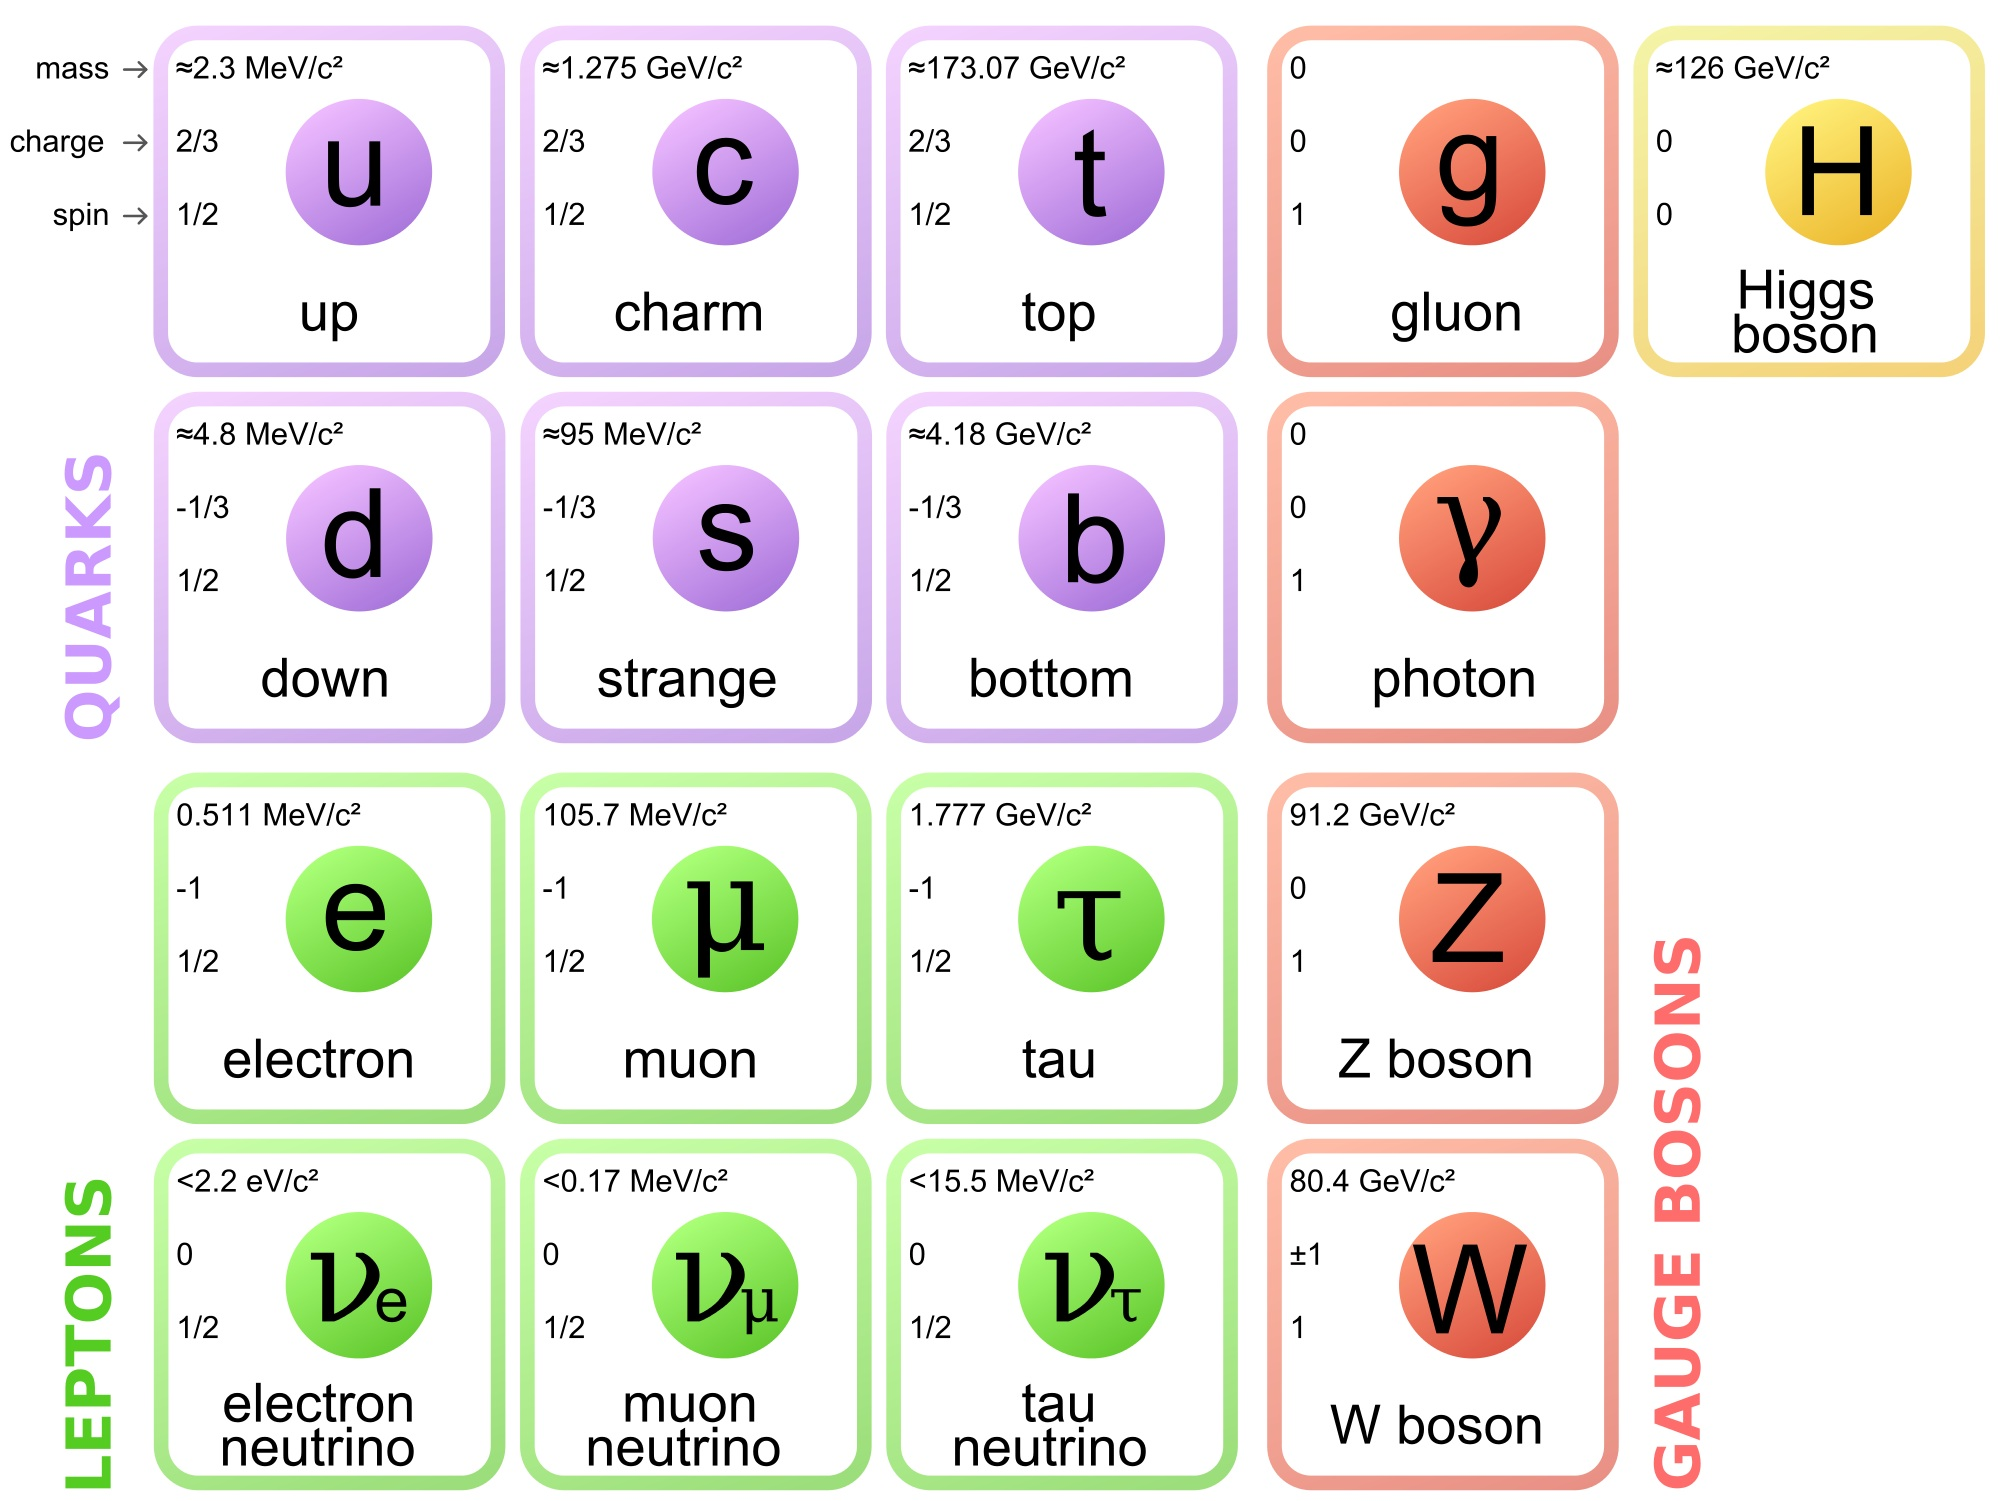
\includegraphics[width=0.8\textwidth]{SM.jpg}\hfill%
  \caption{The particle content of the Standard Model, showing the fermions divided into 3 generations (columns) on the left and the bosons on the right. The electrical charges are expressed as multiples of the absolute value of the electron charge. Figure taken from~\cite{quantumdiaries}.}
  \label{fig:SM}
\end{figure}

A common characteristic of the fermions is their half-integer spin, in contrast to the integer spin of the force mediators, called bosons. Within the Standard Model, the mediation of the different fundamental interactions is represented by the exchange of these spin-1 gauge bosons, which are summarized in Figure~\ref{fig:SM}. The massless photon mediates the most familiar force, the electromagnetic interaction, which is responsible for light, electromagnetic fields, and chemical reactions. The weak nuclear interaction is among other things used to describe the radioactive $\beta$ decay, and is propagated by the neutral $Z$ boson and and two charged massive $W$ bosons. Lastly, the strong nuclear interaction is carried by massless gluons, keeping the protons and neutrons in the atomic nuclei and holding the quark constituents together. A resulting property of the quarks is that they hadronise, i.e. they cannot exist isolated, but form bound states via the strong interaction. These bound states are referred to as hadrons, and can be made up from three quarks or a quark and an antiquark, respectively called baryons and mesons.

Finally, it is also important to note that for every fermion~$(f)$ there exists an antifermion~$(\bar{f})$, which differs only in electric charge and handedness of spin. When matter and antimatter come into contact they annihilate, generating energy which can be transformed into other particles.

\subsection{The theoretical framework of the Standard Model}

The Standard Model goes further than merely giving an exhaustive list of elementary particles, it has a supporting theoretical framework formulated as a relativistic quantum field theory. In a quantum field theory, every particle is represented by discrete excitations of a field $\psi(x)$, where $x$ is the space-time coordinate. The interactions and kinematics of this particle are fully determined by the action $S$, which is defined as the integral of the Lagrangian  $\mathcal{L}(\psi(x), \partial^{\mu}\psi(x))$ over the space-time coordinates:
\begin{equation}
 S = \int\mathcal{L}(\psi(x), \partial^{\mu}\psi(x))d^4x.
\end{equation}
The Lagrangian  is a function of the field $\psi(x)$ and its first derivative $\partial^{\mu}\psi(x)$, where $\mu$ represents the index of the space-time coordinate. The physical behaviour of the particles is obtained by following the principle of least action $\delta S =0$, minimizing the action.

In this framework based on the gauge invariance of the Lagrangian under the fundamental symmetries, the interactions between the fermions and bosons follow automatically. This can be illustrated with the following example for invariance under a general local gauge transformation.

As mentioned before, a fermion has a half integer spin and can thus be represented as a complex relativistic spin-1/2 field, called a Dirac spinor:
\begin{equation}
\label{eq:Ldirac}
 \mathcal{L}_{Dirac} = i\bar{\psi}\gamma^{\mu}\partial_{\mu}\psi - m\bar{\psi}\psi,
\end{equation}
where $\gamma^{\mu}$ are the Dirac matrices, and the adjoint field $\bar{\psi} = \psi^{\dagger}\gamma^0$ is the field associated to the antifermion. The imposed local gauge invariance then requires the fermion fields, and the overall Lagrangian, to be invariant under so-called local phase transformations
\begin{equation}
 \psi \rightarrow \psi' = U(x)\psi = e^{i\vec{\alpha}(x)\cdot\frac{\vec{\tau}}{2}}\psi
\end{equation}
where $\vec{\alpha}(x)$ are the space-time dependent rotation parameters in the symmetry group represented by the Lie group generators $\vec{\tau}$. Since the derivative $\partial_{\mu}$ in (\ref{eq:Ldirac}) spoils the invariance of the Lagrangian under a local phase transformation, it is replaced with a covariant derivative 
\begin{equation}
 D_{\mu} = \partial_{\mu} - ig\frac{\vec{\tau}}{2}\vec{A}_{\mu}, 
\end{equation}
restoring the invariance. This however introduces new vector gauge fields $A_{\mu}$, which interact with the fermion fields with a coupling strength $g$. As a result, the Dirac Lagrangian contains an additional term, which describes the interaction between the fermion fields mediated by the gauge fields $A_{\mu}$, and (\ref{eq:Ldirac}) becomes
\begin{equation}
  \mathcal{L}_{Dirac} = i\bar{\psi}\gamma^{\mu}\partial_{\mu}\psi - m\bar{\psi}\psi + g\bar{\psi}\gamma^{\mu}\psi\vec{A}_{\mu}\cdot\frac{\vec{\tau}}{2}
\end{equation}

The matrix $U(x)$ which was introduced above, was defined as a general rotation matrix of the symmetry group $SU(N)$. In order to obtain the three fundamental interactions of the Standard Model, the described procedure can be simplified using the corresponding symmetry groups as mentioned below.

\begin{itemize}
 \item[] \textbf{Electroweak theory}\\
 The electroweak interaction describes the electromagnetic and weak interactions, which appear very different at low energies but can be merged into a single electroweak force above the electroweak energy scale. This theory is described by requiring gauge invariance under the $SU(2)_L \otimes U(1)_Y$ symmetry group. This leads to 3 gauge fields $W_{\mu}^{\alpha}$ introduced by the $SU(2)_L$ group, and one gauge field $B_{\mu}$ from the $U(1)_Y$ group. Two coupling constants are introduced, $g_1$ and $g_2$, for $U(1)_Y$ and $SU(2)_L$, respectively. The corresponding observable gauge bosons are the photon, the $Z^0$, and the $W^{\pm}$ bosons.
 
 \item[] \textbf{\acf{QCD}}\\
 The strong interaction is described by the theory of \acl{QCD} and is represented by the symmetry group $SU(3)$. It describes the interaction between particles that carry a colour charge, which can be red, green, blue, or one of the three corresponding anticolours. There are eight gauge boson fields associated to this group, which are massless and known as gluons. An important aspect which is unique for this interaction is asymptotic freedom, which states that the strong coupling constant, denoted by $\alpha_s$, goes to zero at high energies. Consequently, the strong force becomes stronger as the distance between the strongly interacting quarks and gluons increases. As a result, the quarks and gluons cannot exist independently and are not observed individually, but are instead confined in colour-neutral hadrons. This effect is called confinement.
\end{itemize}
  
At this point the resulting Lagrangian including the three fundamental forces does not contain any mass terms, and so it cannot explain the observed particle masses. Additional mass terms cannot simply be added explicitly because they would break gauge invariance. Instead, a solution to this problem is found by introducing a complex scalar doublet $\phi$ with a non-zero vacuum expectation value (vev) $v$. This breaks the electroweak symmetry and is known as the Brout-Englert-Higgs (BEH) mechanism, postulated in 1964~\cite{Higgs:1964pj ,Englert:1964et, Guralnik:1964eu}. The Lagrangian of the Higgs field is
 \begin{align}
   \mathcal{L}_H &= (D^{\mu}\phi)^{\dagger}(D_{\mu}\phi) - V(\phi)\nonumber\\
   &= (D^{\mu}\phi)^{\dagger}(D_{\mu}\phi) -\frac{1}{2}\mu^2\phi^{\dagger}\phi + \frac{1}{4}\lambda^2(\phi^{\dagger}\phi)^2,
 \end{align}
where $\mu$ is a real constant representing a mass parameter and $\lambda$ is a dimensionless parameter standing for the self-interaction strength. The potential $V$ of the scalar doublet has an infinite set of minima or ground states, and by choosing a ground state and expanding the field around it, the electroweak symmetry is broken. As a result, three of the four original fields of the scalar doublet are absorbed by the massless vector fields of the weak interaction, giving mass to the $W$ and $Z$ bosons:
\begin{equation}
 M_W = \frac{1}{2}vg_2 \qquad M_Z = \frac{1}{2}v\sqrt{g_1^2 + g_2^2}.
\end{equation}
From the remaining field, the $H$ boson arises, acquiring a mass $m_H = \sqrt{2\lambda v}$.

The introduction of mass terms for the fermions also follows from the BEH mechanism, which allows to insert the following gauge-invariant term in the Lagrangian:
\begin{equation}
  \mathcal{L}_{Yukawa} = -Y_{ij}\bar{\psi}_{L,i}\phi\psi_{R,j} + h.c.
\end{equation}
with the $Y_{ij}$ Yukawa matrices. The $L$ and $R$ here denote left-handed and right-handed fermions. This handedness or chirality is defined as $\psi_{L} = \frac{1}{2}(1-\gamma_5)\psi$ for left-handed and $\psi_{L} = \frac{1}{2}(1+\gamma_5)\psi$ for right-handed fermions. The fermion masses then arise from the Yukawa interactions describing the couplings of the fermions with the Higgs field. For massive particles, a reference frame which overtakes the spinning particle can always be found, in which case the particle will seem to move backwards, flipping its helicity\footnote{The helicity is defined as the sign of the projection of the spin vector onto the momentum vector of a particle, left is negative and right is positive.}. This is however not the case for massless particles, which travel at the speed of light. As only left-handed neutrinos and right-handed antineutrinos have been observed so far, the neutrinos are massless in the Standard Model.

\subsection{Unanswered questions of the Standard Model}

Although the Standard Model is an extremely successful theory, there are still many questions that remain unanswered, indicating that the Standard Model cannot be a complete theory of nature. A brief description of some of the main unsolved problems follows here.
\begin{itemize}
 \item[] \textbf{Grand Unified Theory}\\
 As the weak and electromagnetic interactions were successfully unified into the electroweak one, the idea of representing the three forces of the Standard Model by a single one is envisaged and studied. While this Grand Unified Theory (GUT) could be a first step towards the incorporation of gravity in the Standard Model, it cannot be achieved with the current Standard Model and requires new physics at a very high energy scale.
 
 \item[]\textbf{Baryon asymmetry}\\ 
 This problem refers to the imbalance of matter and antimatter in the universe. While the Big Bang should have produced an equal amount of baryonic and antibaryonic matter, this is not measured in our observable universe. It is assumed that most of the primordial matter and antimatter annihilated, but an imbalance allowed a fraction of the matter to survive. Within the Standard Model, some asymmetry in the production of matter and antimatter could be explained by the CP-violation\footnote{According to Charge Parity (CP) symmetry, the laws of physics should remain identical when converting a particle into its antiparticle and mirroring the space coordinates. However, measurements of e.g. kaon-antikaon mixing show that this symmetry is violated.} of the weak interaction. However, the amount of CP-violation needed to explain the baryon asymmetry is ten times higher than is observed from Standard Model measurements. 
 
 \item[]\textbf{Hierarchy problem}\\ 
 The most important hierarchy problem concerns the question why the weak force is so much stronger than gravity. The measured vector boson masses suggest that the electroweak symmetry breaking should occur at an energy scale of $\mu^2 \sim (100$~GeV$)^2$, while the energy regime where gravity becomes comparable to the other forces, called the Planck scale, is of the order of $\Lambda_{Planck} \sim 10^{19}$~GeV. This question is related to the mystery as to why the Higgs boson mass is so much smaller than the Planck scale. The real physical Higgs boson mass is composed of its bare mass and quantum loop corrections. These corrections depend strongly on a cut-off scale, which would be the Planck scale if no additional physics on top of the Standard Model is present up to this scale. In order for the theoretical prediction to match the experimentally determined mass of 125~GeV, the bare mass would need to be tuned to cancel the huge quadratic radiative corrections. This would require a significant fine-tuning of more than 30 orders of magnitude, which is not desirable for any theory.
 
 \item[]\textbf{Neutrino masses}\\ 
 The Standard Model predicts that the neutrinos are massless weakly interacting particles, but observations by the Sudbury Neutrino Observatory~\cite{Ahmad:2002jz} and Super-Kamiokande~\cite{Fukuda:1998mi} collaborations showed the first clear evidence that the neutrinos oscillate from one flavour into another. This can only be explained if the neutrinos differ in mass, implying that they are not massless. As mentioned above, the Standard Model does not provide masses for the neutrinos and it should therefore be extended to explain this observation.
 
 \item[]\textbf{Dark matter and energy}\\
 This mystery arises from cosmological observations, which indicate that the known matter described by the Standard Model makes up only 5\% of the matter and energy in the universe. The remaining matter, called dark matter, contributes another 27\%, and will be discussed in more detail in Section~\ref{sec:DM}. In the Standard Model, neutrinos contribute to the dark matter, but their relic density is by far not enough to account for all the dark matter. The last 68\% has been labelled dark energy and is believed to be responsible for the acceleration of the observed expansion of the universe, but remains even more enigmatic as no explanation can be provided by the Standard Model.
\end{itemize}

\section{Dark matter}
\label{sec:DM}

One of the current open questions in particle physics that is not answered by the Standard Model is the existence of dark matter. Many astrophysical observations from gravitational effects (see for instance~\cite{Bertone:2004pz}) show there must be some additional matter in the universe, the so-called dark matter, next to the known matter. Despite this, its precise nature remains as of yet unknown. Countless theoretical models are being constructed in order to explain its origin, and on the experimental side dark matter is being looked for in many different ways, but no observation has been made so far.

\subsection{Observational evidence}

The first hints of dark matter were observed by F. Zwicky~\cite{Zwicky:1933gu} in 1933 by studying the velocity dispersion of galaxies in the Coma cluster. The effect is not only observed for entire galaxies, but also for various luminous objects, such as stars or gas clouds, inside a galaxy. The rotation curves of galaxies have been well studied, and show clear evidence for the existence of dark matter. An example of a rotation curve is shown in Figure~\ref{fig:rotationcurves}, exhibiting a flat behaviour of the rotational velocity at large distances, going even far beyond the edge of the visible disk. However, in Newtonian dynamics the circular velocity is expected to be
\begin{equation}
 v(r) = \sqrt{\frac{GM(r)}{r}},
\end{equation}
where $M(r) = 4\pi\int\rho(r)r^2dr$ with $\rho(r)$ the mass density profile. Assuming $M(r)$ to be constant, the circular velocity is expected to fall like $1/\sqrt{r}$ beyond the disk. Since the measurements show an approximately constant velocity but a dropping visible mass density, this implies the existence of a halo with $M(r) \propto r$ and $\rho(r)\propto1/r^2$. A universal density profile seems to be suggested by the rotation curves of both low and high surface luminosity galaxies, consisting of an exponential thin stellar disk and a spherical dark matter halo with a flat core of radius $r_0$ and density $\rho_0 = 4.5\times 10^{-2}(r_0/\textup{kpc})^{-2/3}\textup{M}_\odot\textup{pc}^{-3}$~\cite{Salucci:2002jg}\footnote{$\textup{M}_\odot$ denotes a solar mass, $2 \times 10^{30}$~kg.}.

\begin{figure}[ht]
  \centering
  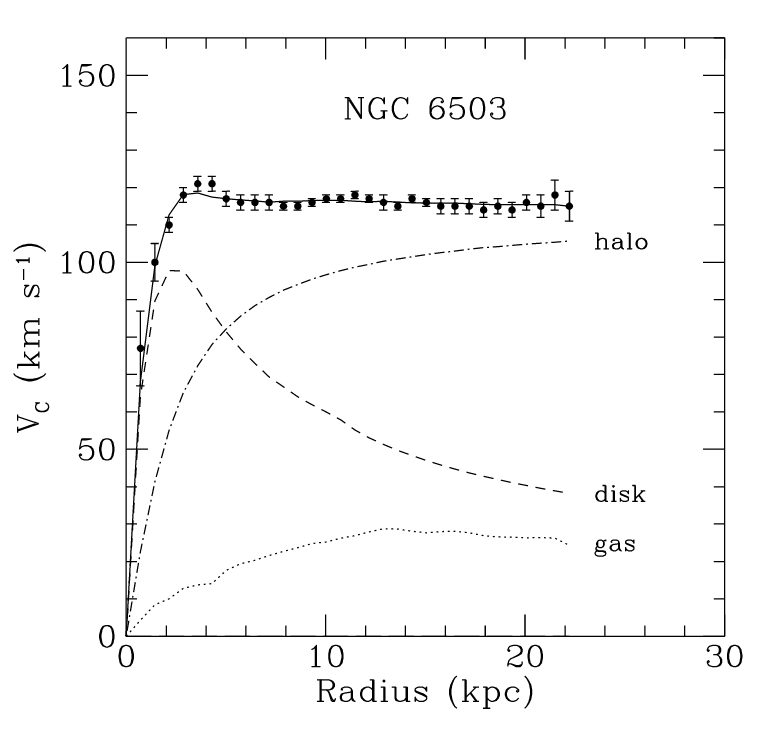
\includegraphics[width=0.6\textwidth]{rotational_curve.png}\hfill%
  \caption{Rotation curve of NGC 6503. The dotted, dashed, and dash-dotted lines show the contributions of gas, disk, and dark matter, respectively. Figure taken from~\cite{Begeman:1991iy}.}
  \label{fig:rotationcurves}
\end{figure}

Another evidence for dark matter comes from the effect of gravitational lensing, allowing to determine the mass of an object regardless of the light it emits. When a distant star or quasar is aligned with a massive compact object, the bending of its light due to the gravitational field of the massive object can 
lead to multiple distorted, magnified, and brightened images, as illustrated in Figure~\ref{fig:gravitational_lensing}. The distortion of the image can then be used to determine the potential well and thus the mass of the heavy object. Yet another way to determine the mass of a cluster of galaxies, next to gravitational lensing and the distribution of radial velocities, is by studying the profile of X-ray emission, tracing the distribution of the hot emitting gas in clusters. In general, these three methods are in reasonable agreement with each other.

\begin{figure}[ht]
  \centering
  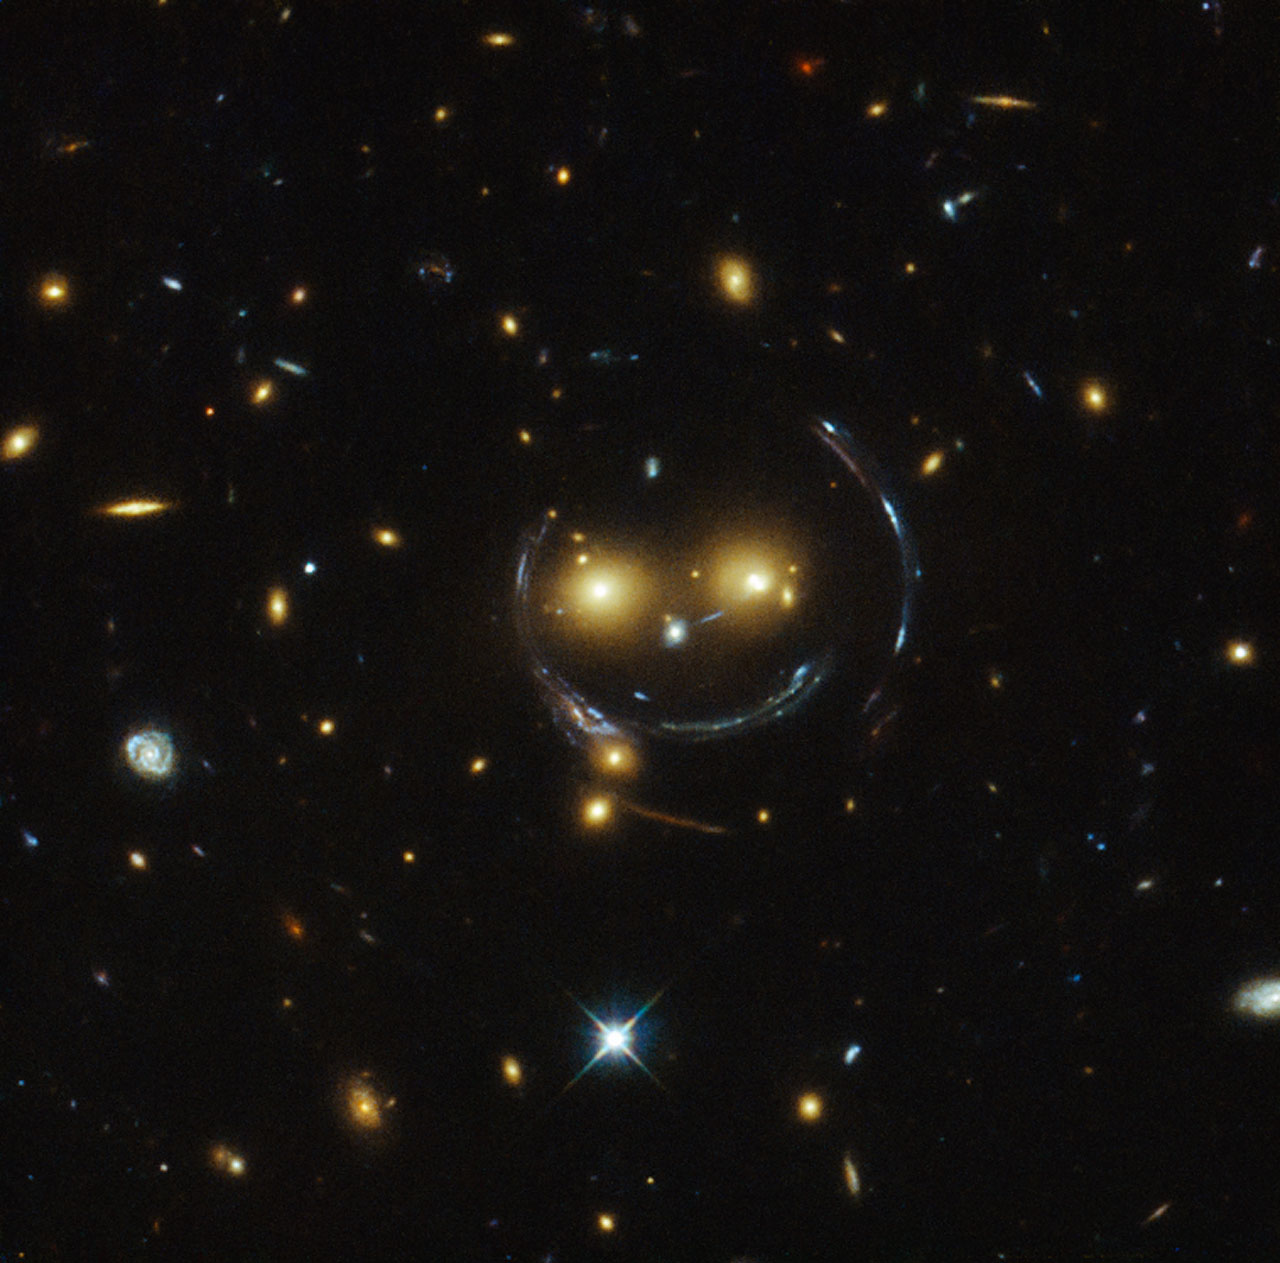
\includegraphics[width=0.65\textwidth]{cat.jpg}\hfill%
  \caption{An example of gravitational lensing showing the ``Cheshire Cat'' image of galaxy cluster  SDSS J1038+4849, taken by the Hubble Space Telescope. Figure taken from~\cite{Belokurov:2008pu}.}
  \label{fig:gravitational_lensing}
\end{figure}

Additionally, at a cosmological level, the analysis of the \ac{CMB} allows to determine the total amount of dark matter in the universe. The existence of this isotropic background radiation was already predicted in 1948, and unintentionally discovered by A. Penzias and R. Wilson in 1965~\cite{Penzias:1965wn}. This relic radiation comes from the propagation of photons in the early universe, once they decoupled from matter. Before this, the photons were energetic enough to ionise hydrogen, creating a plasma of electrons and protons which were unable to combine into hydrogen. As the universe expanded and cooled down, the photons also cooled down enough to let the hydrogen atoms recombine, and the universe became transparent. The photons can then travel freely without scattering off the protons and electrons of the plasma, still carrying information from this surface of last scattering. The \ac{CMB} is now known to be isotropic at the level of $10^{-5}$ and to follow the spectrum of a black body corresponding to a temperature of 2.726~K. However, small anisotropies in the \ac{CMB} have first been observed by the COBE satellite~\cite{Smoot:1992td} and more recently by WMAP~\cite{Komatsu:2010fb} and Planck~\cite{Ade:2013zuv}, as can be seen in Figure~\ref{fig:CMB}. These anisotropies correspond to small thermal variations, and are usually expanded as
\begin{equation}
 \frac{\delta T}{T}(\theta, \phi) = \sum_{l=2}^{+\infty}\sum_{m=-l}^{+l} a_{lm} Y_{lm}(\theta, \phi), 
\end{equation}
where $Y_{lm}(\theta, \phi)$ are spherical harmonics. % EB: sounds a bit slangy
The variance of $a_{lm}$ is given by
\begin{equation}
 C_l = \left\langle|a_{lm}|^2\right\rangle = \frac{1}{2l+1}\sum_{m=-l}^{+l} 
|a_{lm}|.
\end{equation}
As the temperature fluctuations appear to be Gaussian, all the information contained in the \ac{CMB} anisotropy maps can be condensed into the power spectrum given by the behaviour of $C_l$ as a function of $l$. This is generally represented using $D_l = l(l+1)C_l/2\pi$, as illustrated in Figure~\ref{fig:powerspectrum}.

\begin{figure}[ht]
  \centering
  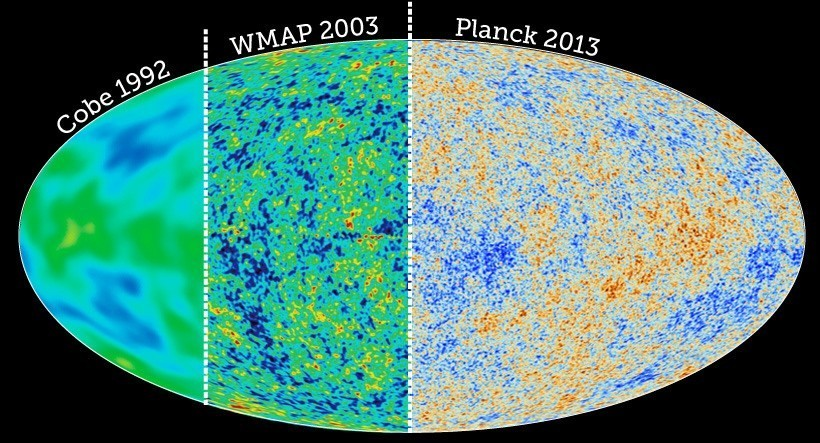
\includegraphics[width=0.8\textwidth]{cmb1.jpg}\hfill%
  \caption{The \ac{CMB} temperature fluctuations obtained from the COBE, WMAP, and Planck data. Figure taken from~\cite{CMB}.}
  \label{fig:CMB}
\end{figure}

\begin{figure}[ht]
  \centering
  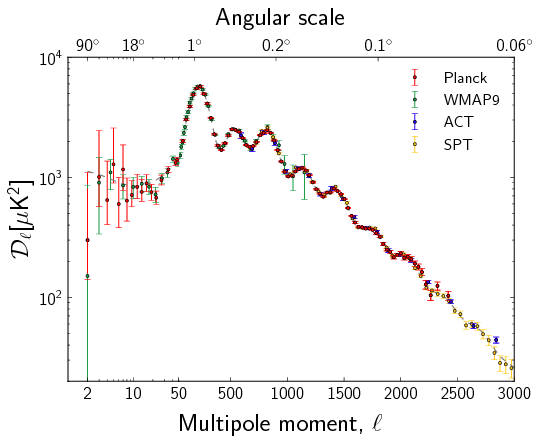
\includegraphics[width=0.8\textwidth]{power_spectrum.png}\hfill%
  \caption{The observed power spectrum of the \ac{CMB} anisotropies. The horizontal axis is logarithmic up to $l = 50$ and linear beyond. Figure taken from~\cite{Ade:2013sjv}.}
  \label{fig:powerspectrum}
\end{figure}

The \ac{CMB} anisotropies are caused by acoustic oscillations arising from the conflict between the gravitational pull from baryons and dark matter and the repulsive force due to the radiation pressure from the photons. One popular model to describe and interpret the these observations is the $\Lambda$CDM model. CDM stands for cold dark matter, indicating that in this model the dark matter particles are moving slowly compared to the speed of light, while the $\Lambda$ represents the cosmological constant, which is associated with the vacuum energy or dark energy that is used to explain the accelerating expansion of space. The $\Lambda$CDM model is compatible with a number of observations beyond the \ac{CMB} fluctuations, such as the large scale structure in the distribution of galaxies, the relative abundance of light nuclei, and the accelerating expansion of the universe which is observed from the red shift of well-known spectral absorption or emission lines in the light of distant galaxies. Using this model to fit the power spectrum, the multiple peaks in the spectrum can be interpreted. The angular scale of the first peak can be used to determine the curvature of the universe. The second peak determines the reduced baryon density and the third peak can be used to retrieve information about the dark matter density. From the analysis of the Planck data the abundance of baryons and matter in the universe is determined to be
\begin{equation}
 \Omega_b h^2 = 0.02205 \pm 0.00028 \qquad \Omega_M h^2 = 0.1423 \pm 0.0029
\end{equation}
This result shows that only about 15\% of the matter in the universe is made up from the ordinary known matter, and the remaining 85\% is called dark matter.

More evidence for dark matter was found from a great variety of data, both on subgalactic and inter-galactic scales. Without discussing them here in detail, a few examples are the velocity dispersions of spiral galaxy satellites, suggesting the existence of dark halos around spiral galaxies extending well beyond the visible disk~\cite{Azzaro:2003hp}, the velocity dispersion of dwarf spheroidal galaxies, implying larger mass-to-light ratios than those observed in our local neighbourhood~\cite{Mateo:1998wg}, and the so-called Oort discrepancy in the disk of the Milky Way, inferring the existence of dark matter from the inconsistency between the amount of stars in the solar neighbourhood and the gravitational potential indicated by their distribution~\cite{Bahcall:1991qs}.

\subsection{Dark matter models}

Since very little is know so far concerning the nature of dark matter, a multitude of dark matter candidates are discussed in the literature. Without attempting to be complete, a list is given and a few of the more popular candidates are briefly covered here.

\begin{itemize}
 \item[] \textbf{Standard Model neutrinos}\\
	As mentioned before, the Standard Model could explain the existence of dark matter with the already observed neutrinos. However, it can be shown~\cite{Bergstrom:2000pn} that their total relic density is predicted to be 
	\begin{equation}
	 \Omega_{\nu}h^2 = \sum_{i = 1}^3 \frac{m_i}{93\ \mathrm{eV}},
	\end{equation}
	taking the sum over the 3 neutrino flavours. Currently, the most stringent upper bound on neutrino masses is
	\begin{equation}
	 m_{\nu} < 2.05\ \text{eV \hspace{.3cm} at 95\% CL}
	\end{equation}
	obtained in tritium $\beta$-decay experiments at Troitsk~\cite{Lobashev:2003kt,Aseev:2011dq} and Mainz~\cite{Kraus:2004zw}. Since the mass difference between the 3 neutrinos must be very small to explain solar and atmospheric neutrino anomalies~\cite{GonzalezGarcia:2002dz}, this mass limit applies to the three mass eigenvalues, implying an upper bound on the total neutrino relic density of 
	\begin{equation}
	  \Omega_{\nu}h^2 \lesssim 0.07.
	\end{equation}
	This shows that Standard Model neutrinos are not abundant enough to be the dominant component of dark matter.
	
 \item[] \textbf{Sterile neutrinos}\\
         Proposed in 1993 by Dodelson and Widrow~\cite{Dodelson:1993je}, these hypothetical particles are similar to the Standard Model neutrinos, but without Standard Model weak interactions, except for mixing. The analysis of their cosmological abundance and the study of their decay products places stringent constraints on the sterile neutrinos. Light neutrinos with masses below a few keV would for example be ruled out~\cite{Yoshida:2003rm}.
         
 \item[] \textbf{Axions}\\
         These particles were originally introduced to solve the problem of the apparent absence of CP-violation by the strong interaction, and have often been discussed as dark matter candidates. They are expected to interact extremely weakly with Standard Model particles. Furthermore, observations from laboratory searches, stellar cooling, and the dynamics of supernova 1987A constrain the axion mass to be very small, of the order of or below 0.01~eV~\cite{Rosenberg:2000wb}.
         
 \item[] \textbf{\acs{SUSY} candidates}\\
         Several particles in \ac{SUSY} models can serve as dark matter candidate, such as gravitinos and neutralinos. Gravitinos are the superpartners of the graviton. In some \ac{SUSY} models, they can be the lightest supersymmetry particle and can be stable. While they are very strongly motivated theoretically, they are very difficult to observe, as they only interact gravitationally. The neutralinos are the superpartners of the photon, $Z$ boson, and neutral Higgs bosons. The lightest of the four is stable and is an excellent dark matter candidate. These dark matter candidates are often called \acp{WIMP}, since they are massive and interact through the weak interaction. As many \ac{SUSY} models predict a new particle with the correct properties and self-annihilation cross section to obtain the correct abundance of dark matter today, a stable supersymmetric partner has long been a very plausible dark matter candidate and a lot of experimental effort has been made to detect it.
         
 \item[] \textbf{\acp{WIMP}}\\         
         A prevalent assumption is that dark matter particles are a relic from the early universe, when all particles were in thermal equilibrium. At those high energies the dark matter particles and antiparticles could be formed by sufficiently energetic lighter particles, and they would annihilate back into these lighter particles as well. However, as the universe expanded and cooled down, the thermal energy of the lighter particles became insufficient to form dark matter particle-antiparticle pairs. The annihilation of the dark matter particles and antiparticles continued however, until the dark matter density decreased considerably and the interaction between the dark matter particles stopped. The number of dark matter particles would remain constant from that moment on. In comparison, particles with a large interaction cross section would continue to annihilate for a longer period of time and would be less abundant. 
         
         The interaction cross section of the annihilating dark matter particles can be inferred from the current estimates of the dark matter abundance in the universe, and can in this case not be larger than the cross section of the weak interaction. According to this model, \acp{WIMP} would be the perfect candidates for dark matter. In general, they are hypothetical new elementary particles that interact gravitationally and through any other force which is as weak or weaker than the Standard Model weak interaction, and they could have been produced thermally as described in this model. Since \acp{WIMP} have a relatively large mass, they would also constitute cold dark matter, which would fit the observed large scale structure of the universe. The coincidence of \acp{WIMP} fitting so well into this model and corresponding to the current observations is known as the ``\ac{WIMP} miracle''.
         
%          het standaard verhaal van de thermal freeze-out (Boltzmann vergelijking, <sigma v>,...), en dus deze figuur:
% https://www.google.it/search?q=freeze+out+dark+matter&client=ubuntu&hs=m3z&channel=fs&dcr=0&source=lnms&tbm=isch&sa=X&ved=0ahUKEwjl1vWR9P_WAhVrCMAKHbVBDI0Q_AUICigB&biw=1337&bih=728
% 
% Ik weet ook niet of je ergens zegt waarom warm dark matter problematisch is. Maar dat kan er ook later nog bij.
         
\end{itemize}

Many more dark matter candidates are discussed in literature, such as but not limited to heavy fourth generation neutrinos~\cite{Kainulainen:2002pu}, Kaluza-Klein states in ADD~\cite{ArkaniHamed:1998rs} or RS~\cite{Randall:1999ee} extra dimensions models, superheavy dark matter or Wimpzillas~\cite{Kolb:1998ki}, self-interacting dark matter~\cite{Spergel:1999mh}, charged massive particles (CHAMPs)~\cite{DeRujula:1989fe}, and Q-balls~\cite{Kusenko:1997si}. More detailed reviews are given in~\cite{Ellis:1998gt,Bergstrom:2000pn,Bergstrom:2009ib}.

\subsection{Detection of dark matter}

The detection of dark matter can be categorised in three groups, based on the diagram shown in Figure~\ref{fig:DM_production}. In the case of direct detection experiments, the studied process is the scattering of dark matter off ordinary matter. Experiments searching for dark matter with the indirect approach look for particles or radiation produced in the annihilation of dark matter particles. Finally, at collider experiments, attempts are made to produce and detect dark matter particles by colliding Standard Model particles at high energies.

\begin{figure}[ht]
  \centering
  \includegraphics[width=0.35\textwidth]{DM_production.pdf}\hfill%
  \caption{Diagram illustrating the three used methods to detect dark matter.}
  \label{fig:DM_production}
\end{figure}

\subsubsection{Direct detection experiments}

This category of experiments is based on the fact that if our galaxy is filled with a static halo of dark matter particles, then many of them should pass through the Earth as it rotates around Galactic Center, and they could be detected by looking for the interaction of such particles with matter. This is for example done by recording the recoil energy of nuclei when \acp{WIMP} scatter off them. In order to determine the expected rate of events per unit detector material mass, the \ac{WIMP}-nucleon scattering cross section and the density and velocity distribution of the \acp{WIMP} in the solar neighbourhood are needed.

There are several types of scattering processes which can be classified by two relevant characteristics: elastic or inelastic scattering and spin-dependent or spin-independent scattering. In the case of elastic scattering, the \ac{WIMP} simply scatters off a nucleus as a whole, causing it to recoil. The recoil energy spectrum can then be measured by detecting the emitted scintillation light with very sensitive detectors or by measuring very small temperature changes due to crystal vibrations. Taking a Maxwell-Boltzmann velocity distribution with as characteristic velocity our rotation velocity of about 270 km/s, the recoil spectrum is exponential with typical energies of $\left\langle E \right\rangle \sim 50$~keV. This range of energies is easily detectable by current experiments, which can detect recoils as low as 1-10~keV. Instead, when the \ac{WIMP} scatters inelastically, it interacts with the orbital electrons of the target, exciting the electrons or ionising the target. Differently, the \ac{WIMP} could also excite the target nuclei, which would then emit a photon about a nanosecond after the observed recoil. This signature has, however, to compete with the background from natural radioactivity.

The spin dependence or independence of the scattering depends on the coupling of the \acp{WIMP} to the Standard Model particles. Spin-dependent interactions result from couplings to the spin content of a nucleon, yielding cross sections that are proportional to J(J+1) instead of the number of nucleons. For spin-independent interactions, the cross section instead increases considerably with the mass of the target nuclei. The spin-independent scattering therefore dominates over the spin-dependent one in experiments which use heavy atoms.

Numerous direct detection experiments are currently operational or in development. They use one or more techniques to measure the nuclear recoil, by detecting the scintillation light, the change in temperature, or the ionisation. Some experiments also try to separate the \ac{WIMP} signatures from the background by looking for an annual modulation in the rate, which arises due to the Earth's movement around the Sun. This effect causes the Earth to have a relative velocity with respect to the galaxy's reference frame, given by 
\begin{equation}
v_E = 220\mathrm{km/s}\left(1.05+0.07\cos(2\pi(t-t_m))\right),
\end{equation}
where the time is in units of years and $t_m$ is approximately the beginning of June. As a result, a small variation of about 7\% in the \ac{WIMP} flux can be measured in the direct detection rate. 

Currently, there is some tension between the results obtained by the different experiments, as some observations can be interpreted as dark matter signals, while other experiments are ruling out those models. The DAMA experiment for example observes an annual modulation in the event rate, pointing to the existence of \acp{WIMP} scattering elastically off the sodium and iodine nuclei in the detector~\cite{Bernabei:2013xsa}. 
%However, other experiments are in tension with the various dark matter interpretations of this signal. 
% Similarly, the CoGeNT experiment observes an annual rate modulation as well~\cite{Aalseth:2014eft}. The phase of the signal corresponds to the phenomenological expectation for a \ac{WIMP} at the level of $2.2\sigma$, but the amplitude of the signal is a factor 4 to 7 larger than expected. 
Other experiments, such as SuperCDMS~\cite{Agnese:2014aze}, EDELWEISS-III~\cite{Armengaud:2016cvl}, CRESST-II~\cite{Angloher:2014myn}, XENON100~\cite{Aprile:2016swn}, have seen no evidence for dark matter so far and placed limits on many dark matter models, creating a tension with the observed signal at DAMA. For \ac{WIMP} masses above a few GeV, the strongest limit of direct detection experiments for spin-independent interactions is currently given by LUX~\cite{Akerib:2016vxi}. For a spin-dependent \ac{WIMP}-proton cross section, the most stringent limit is set by the PICO experiment~\cite{Amole:2017dex}, while the PandaX experiment places the strongest limit on the \ac{WIMP}-neutron cross section~\cite{Fu:2016ega}. An overview of the existing limits and signal observations is given in Figure~\ref{fig:direct_detection}, showing the mentioned experiments, and a more complete review of the existing direct detection results is given in~\cite{Undagoitia:2015gya}.

\begin{figure}[ht]
  \centering
  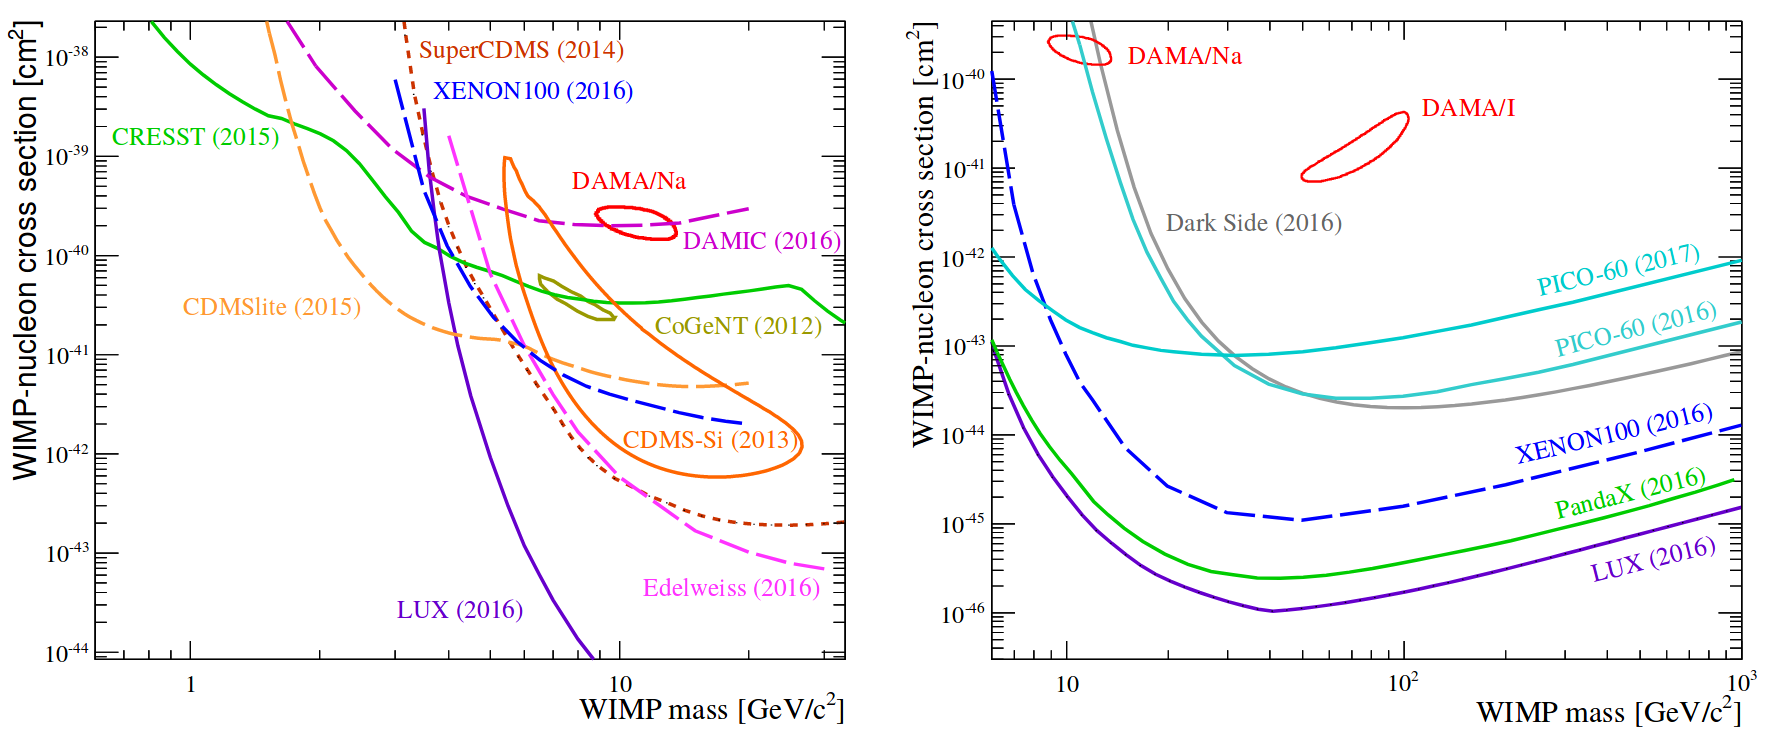
\includegraphics[width=\textwidth]{spinindependent.png}\\
  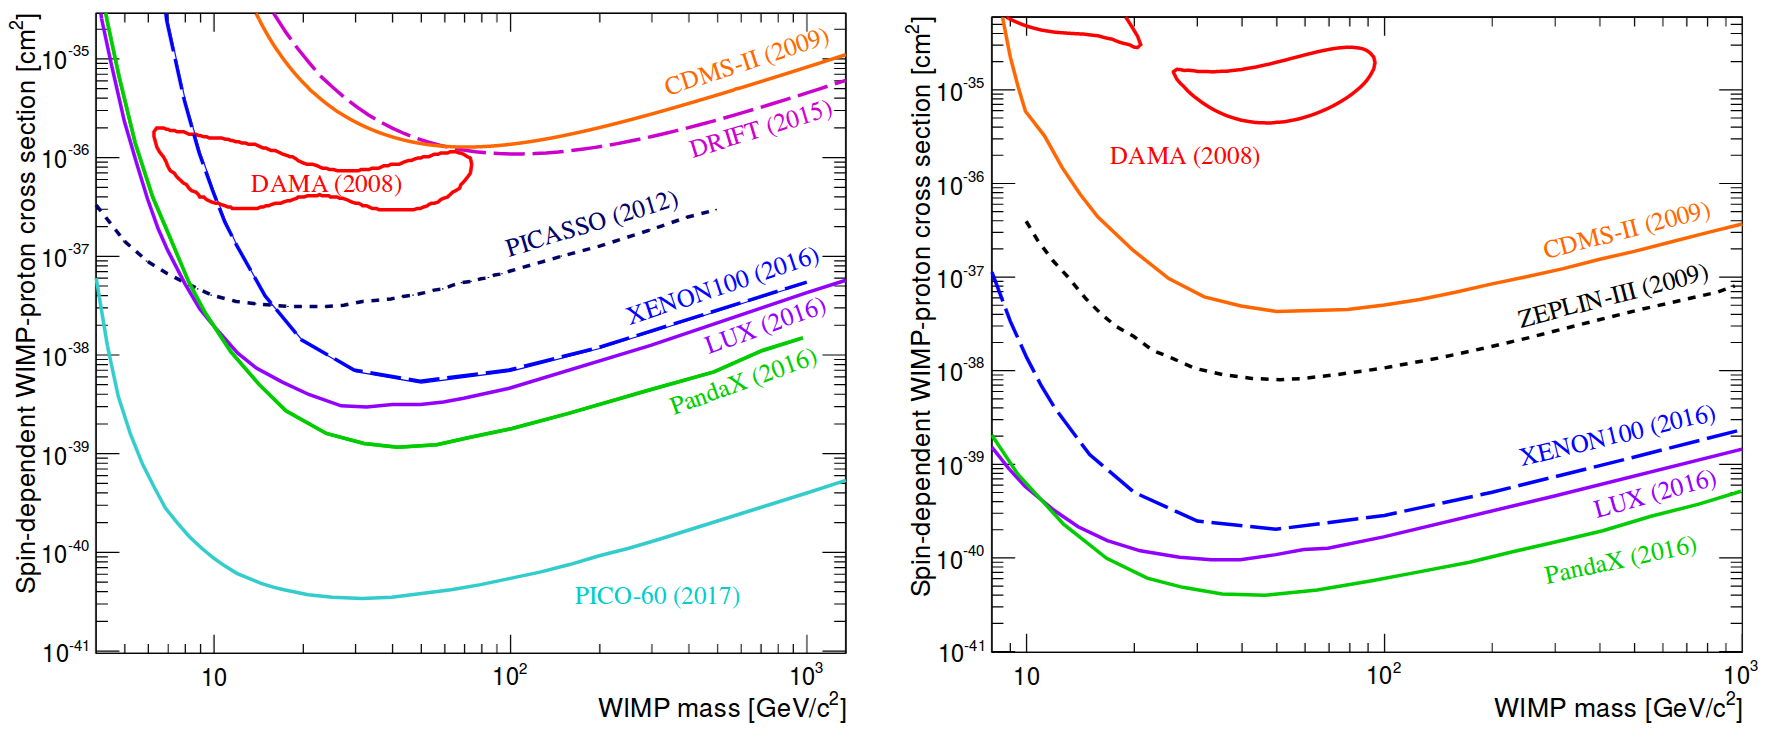
\includegraphics[width=\textwidth]{spindependent.png}\hfill%
  \caption{Overview of the current limits for spin-independent \ac{WIMP}-nucleon interactions at low (top left) and high (top right) \ac{WIMP} masses, spin-dependent \ac{WIMP}-proton interactions (bottom left), and spin-dependent \ac{WIMP}-neutron interactions (bottom right). The observed signals from DAMA, CoGeNT, and CDMS-Si are shown as well. Figure taken from~\cite{Undagoitia:2015gya}.}
  \label{fig:direct_detection}
\end{figure}

\subsubsection{Indirect detection experiments}

The indirect detection of dark matter is performed by looking for radiation produced in dark matter annihilations. A reasonable place to look at would then be in regions with large dark matter densities and thus larger annihilation rates, which will result in a higher flux of the studied radiation. Some examples are dense regions of the galactic halo such as the galactic centre, or objects like the Sun or the Earth, which could also capture dark matter particles through scattering with nucleons in their core. In the latter case, only neutrinos would be able to escape those dense objects. Other annihilation products include gamma rays, positrons, and antiprotons.

In order to observe gamma rays directly, the detectors must be placed in space, as photons of the relevant energy range (GeV to TeV) interact with matter via $e^+e^-$ pair production and cannot traverse more than a surface density of about 38~g~cm$^{-2}$. The gamma rays will not reach the ground-based telescopes as the Earth's atmosphere is 1030~g~cm$^{-2}$ thick. Nevertheless, efforts are being made to observe gamma rays indirectly via ground-based experiments as well, by detecting the secondary particles and the Cherenkov light produced by their passage through the Earth's atmosphere. In the energy range between approximately 100~MeV and 100~GeV, gamma ray telescopes on satellites such as the Fermi Large Area Telescope~\cite{Atwood:2009ez} are being used. Above 100~GeV, the ground-based Imaging Air Cherenkov Telescopes such as HESS~\cite{Aharonian:2006pe}, MAGIC~\cite{Aleksic:2011bx}, and VERITAS~\cite{Holder:2008ux} become more adequate.

Neutrinos can also be produced in the annihilation of dark matter particles, but they are considerably more difficult to detect than gamma rays due to their weak interaction with ordinary matter. They are not easily absorbed, which makes it possible to observe them with underground, low-background experiments. Very energetic neutrinos, in the GeV-TeV range, are most easily observed by detecting the Cherenkov light from muons produced through charge current interactions of the neutrinos inside of or close to the detector volume. Two very large neutrino detectors are ANTARES in the Mediterranean Sea~\cite{Collaboration:2011nsa} and IceCube at the South Pole~\cite{Achterberg:2006md}.

Additionally, evidence for dark matter annihilations can also be found by studying the spectra of cosmic positrons and antiprotons. Contrary to neutrinos and gamma rays, these charged particles do not point to their source, as their trajectory is modified by the presence of galactic magnetic fields. Currently, the main detector for positrons and antiprotons is AMS~\cite{Kounine:2012ega}, which is operating on the International Space Station. Until 2016, PAMELA~\cite{Picozza:2006nm} was also active on board of the Resurs-DK1 satellite.

Finally, radio emissions from the galactic halo, and in particular from the galactic centre, can also provide evidence for dark matter annihilation. Electrons and protons produced in dark matter annihilations will emit synchrotron radiation at radio wavelengths as they move through galactic magnetic fields. This type of searches is performed with radio telescopes and belongs to the realm of classical astronomy.

\subsubsection{Collider experiments}

Since dark matter particles are usually assumed to be neutral and to interact only weakly with ordinary matter, they are expected to pass through the detectors at colliders without leaving a signal, similar to neutrinos. These particles can however still be searched for at colliders as well, when they are produced in association with other visible particles which are detected as jets or charged leptons. The dark matter particles are then observed as missing energy, as they create an imbalance in the net momentum in the transverse plane perpendicular to the colliding beams, which should be zero. One of these flagship analyses is the monojet analysis, looking for dark matter produced together with one or more jets\cite{Sirunyan:2017hci,Aaboud:2016qgg}. Similarly, many more searches are performed at the \acs{CMS} and \acs{ATLAS} experiments at the \ac{LHC} by looking for signatures containing missing energy. Recent summaries are given in~\cite{Kahlhoefer:2017dnp} and \cite{Buchmueller:2017qhf}.

Additionally, other signatures without missing energy can also be used to search for dark matter. If the dark matter particle is produced in a cascade of decays for example, different signatures can be obtained, such as displaced vertices~\cite{ATLAS:2017bvh}, disappearing tracks~\cite{ATLAS:2017bna}, and displaced lepton-jets~\cite{ATLAS:2017lvz}. Furthermore, in dijet searches~\cite{Sirunyan:2017ygf, Sirunyan:2016iap, Aaboud:2017yvp}, resonances in the mass spectrum are being looked for, as this could point to the existence of a new dark matter mediator. If the dark matter particles couple to quarks via a dark matter mediator, this mediator can either decay to a pair of dark matter particles or a pair of Standard model quarks which can be observed as a pair of jets.  Finally, for some particular types of dark matter candidates, such as \acfp{SIMP}~\cite{Bai:2011wy} or \acp{HSCP}~\cite{CMS:2016ybj,Aaboud:2016dgf}, more unusual signatures are expected. This is currently a developing area of dark matter research, and more and more searches looking for new signatures are appearing.

% Many searches for dark matter exist, and the most recent ones are being performed by experiments at the \ac{LHC}. 
In Figures~\ref{fig:summary_SD} and \ref{fig:summary_SI}, recent limits from dark matter searches at the \acs{CMS} experiment are compared to the direct detection results, for spin-dependent and spin-independent interactions, respectively.

\begin{figure}[p]
  \centering
  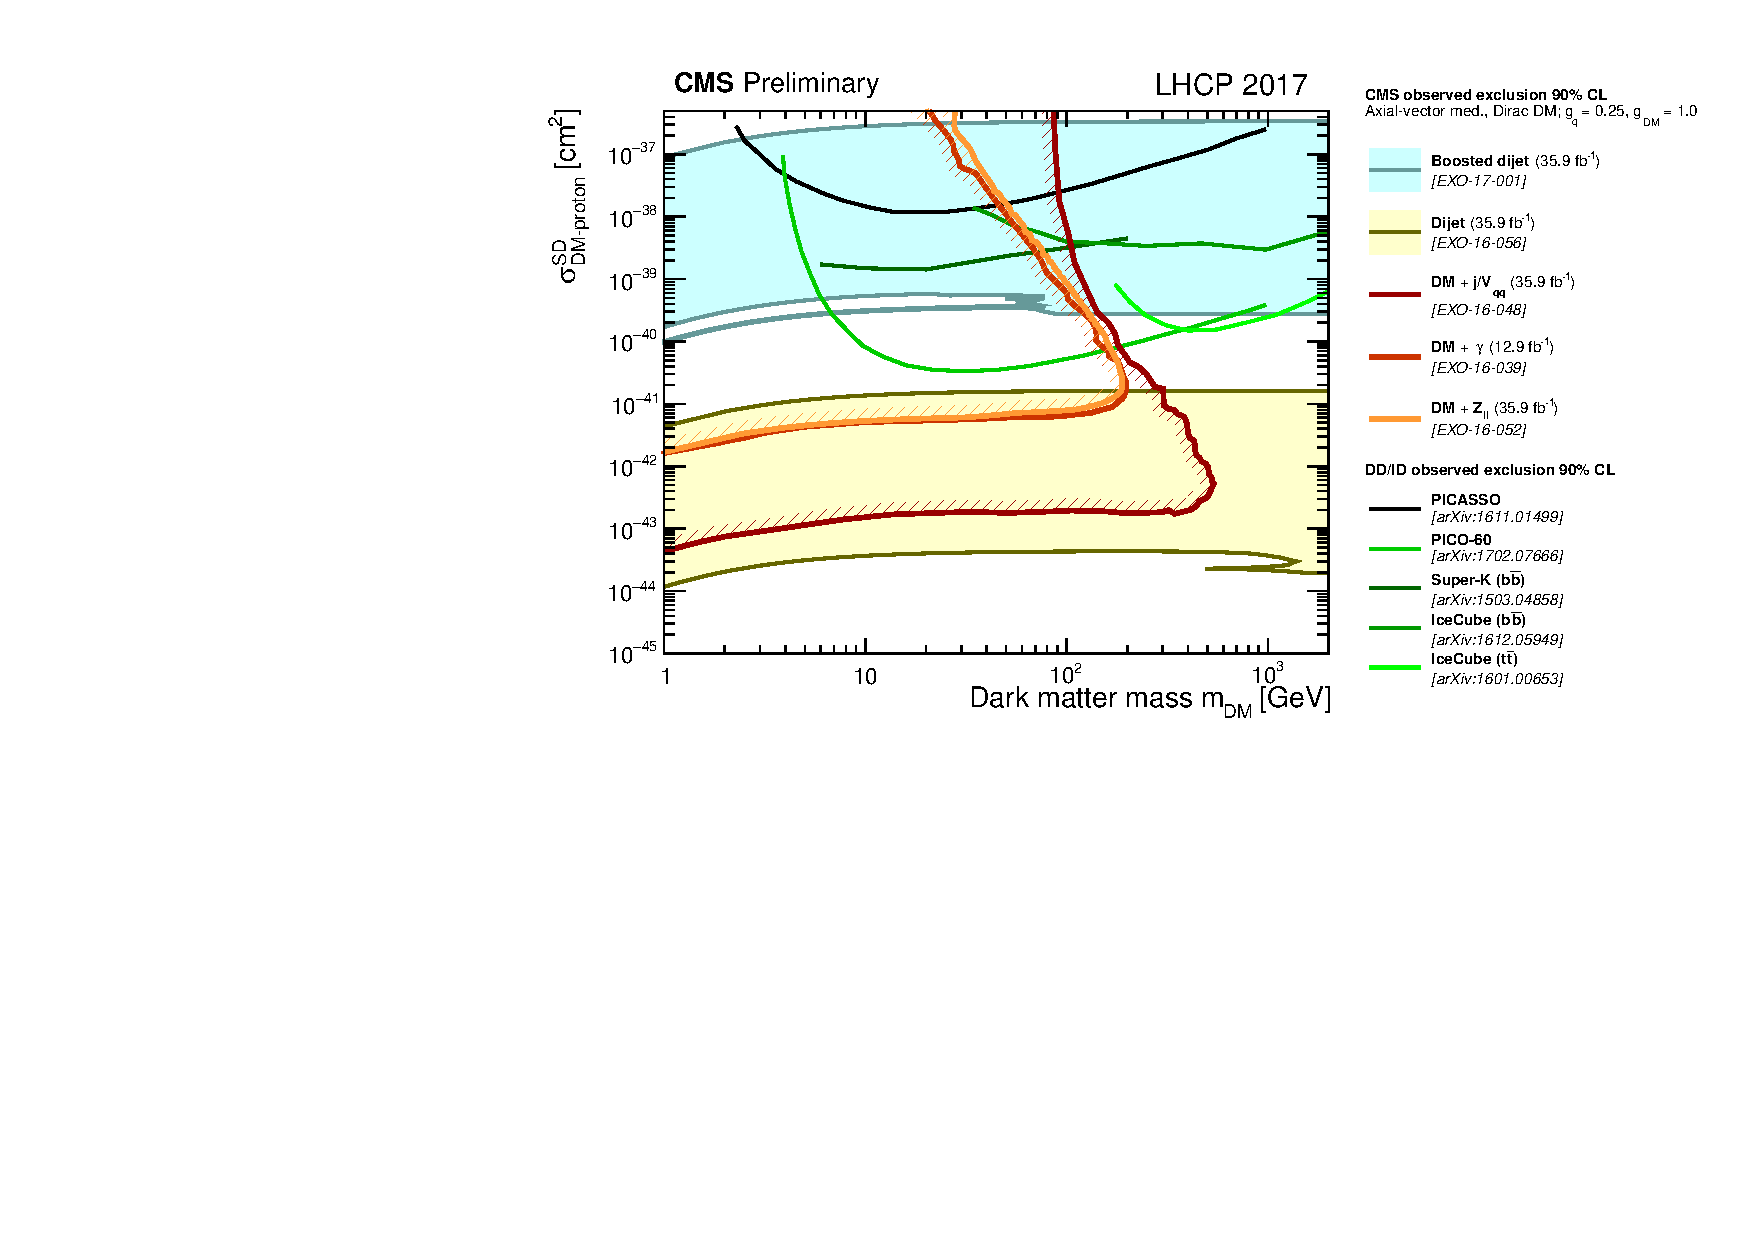
\includegraphics[width=\textwidth]{SD_CMSDD_Summary.pdf}\\
  \caption{A comparison of \protect \acs{CMS} results to direct detection experiments in the $\protect\mathrm{m_{DM}}-\sigma_{\mathrm{SD}}$ plane. The limits are shown at $90\%$ CL. The shown \protect \acs{CMS} contours are for an axial-vector mediator with Dirac dark matter and couplings $g_q=0.25$ and $\protect g_{\mathrm{DM}} = 1.0$. The spin-dependent exclusion contours are compared with limits from the PICASSO and PICO experiments, the IceCube limit for the $\protect t\bar{t}$ and $\protect b\bar{b}$ annihilation channels, and the Super-Kamiokande limit for the $\protect b\bar{b}$ annihilation channel.  It should be noted that the \protect \acs{CMS} limits do not include a constraint on the relic density and also the absolute exclusion of the different \protect \acs{CMS} searches as well as their relative importance will strongly depend on the chosen coupling and model scenario.  Therefore, the shown \protect  \acs{CMS} exclusion regions in this plot are not applicable to other choices of coupling values or models. Figure taken from~\cite{DMsummary}.}
  \label{fig:summary_SD}
\end{figure}

\begin{figure}[p]
  \centering
  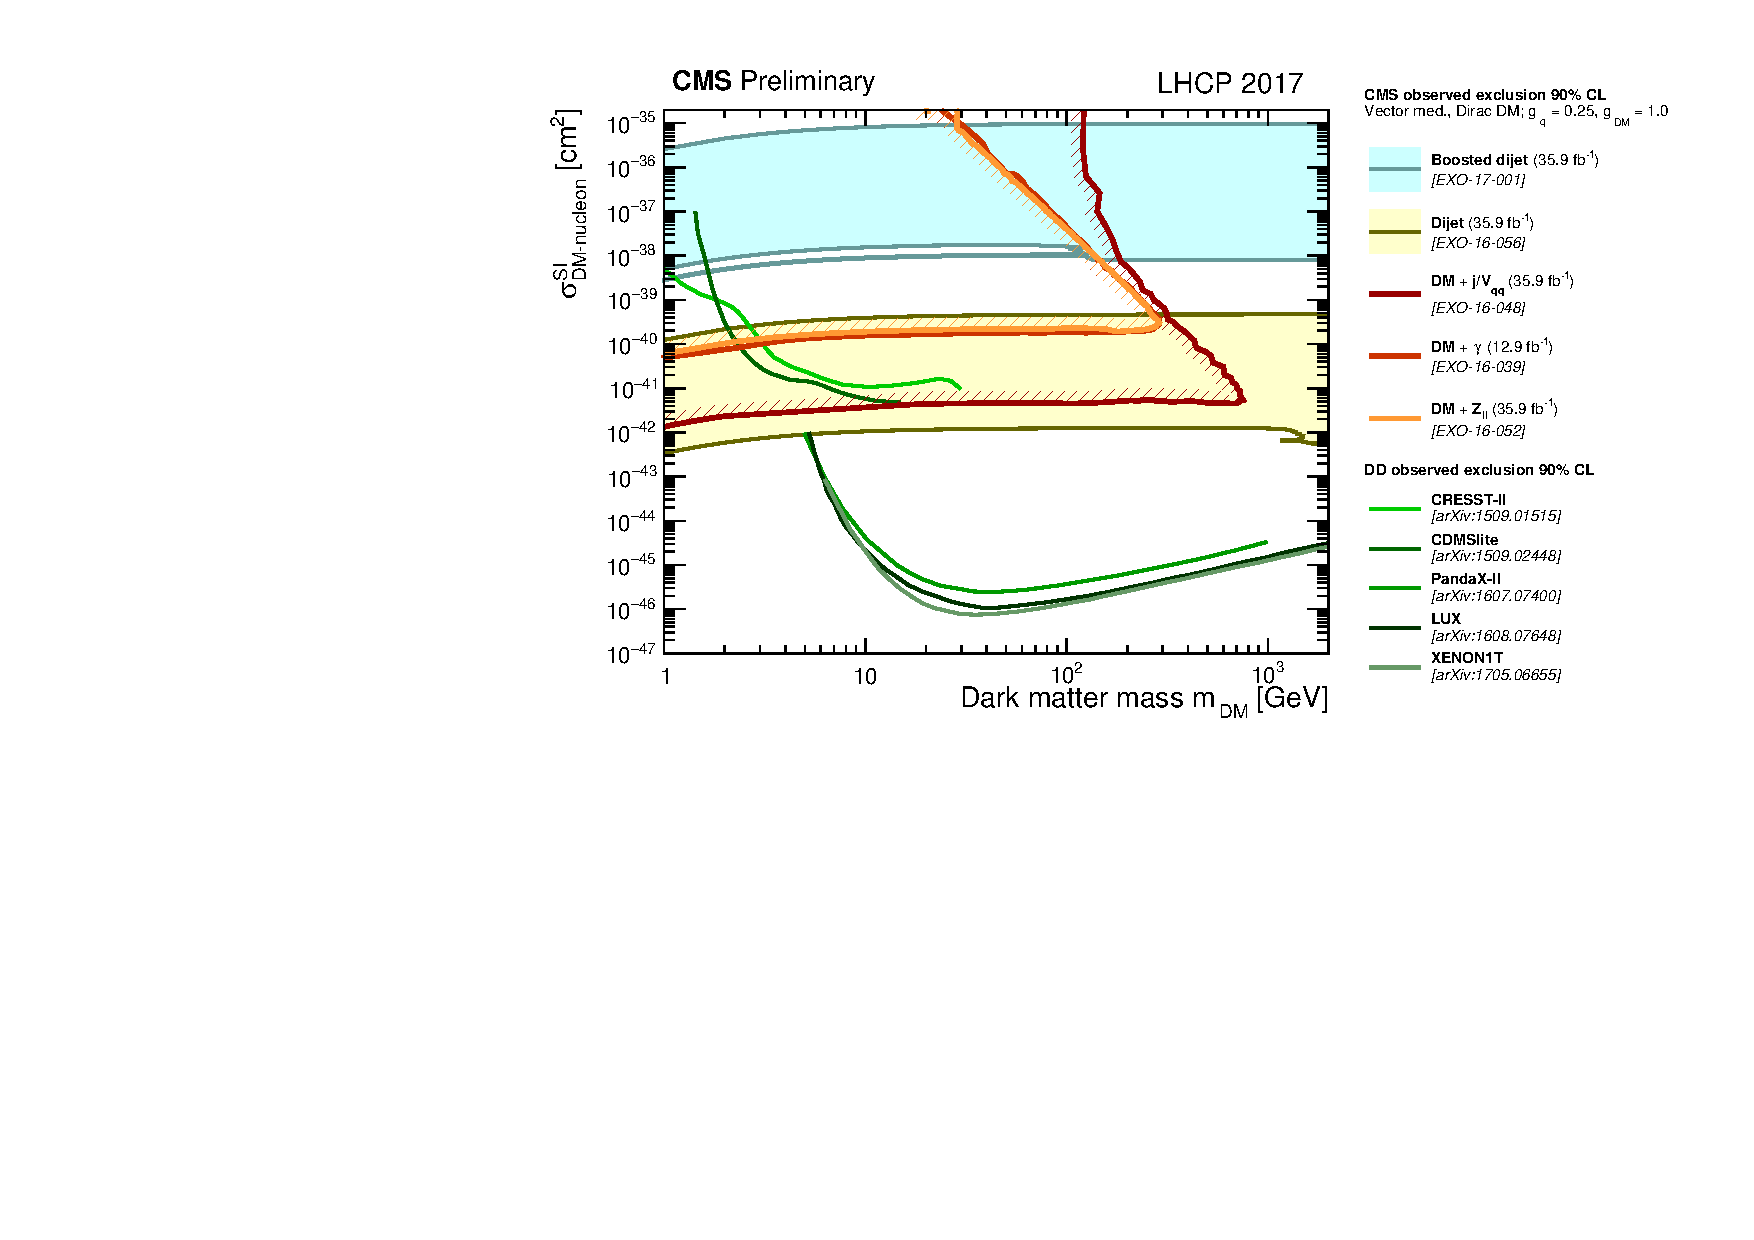
\includegraphics[width=\textwidth]{SI_CMSDD_Summary.pdf}
  \caption{A comparison of \acs{CMS} results to direct detection experiments in the $\protect\mathrm{m_{DM}}-\sigma_{\mathrm{SI}}$ plane. The limits are shown at 90\% CL. The shown \acs{CMS} contours are for a vector mediator with Dirac dark matter and  couplings $g_q=0.25$ and $\protect g_{\mathrm{DM}} = 1.0$. The spin-independent exclusion contours are compared with the XENON1T 2017, LUX 2016, PandaX-II 2016, CDMSLite 2015 and CRESST-II 2015 limits, which constitutes the strongest documented constraints in the shown mass range. It should be noted that the \acs{CMS} limits do not include a constraint on the relic density and also the absolute exclusion of the different \acs{CMS} searches as well as their relative importance will strongly depend on the chosen coupling and model scenario.  Therefore, the shown \acs{CMS} exclusion regions in this plot are not applicable to other choices of coupling values or models. Figure taken from~\cite{DMsummary}.}
  \label{fig:summary_SI}
\end{figure}

\subsection{From EFTs to simplified models}

In order to efficiently look for dark matter at colliders, effective field theories (EFTs) have been used extensively to model the dark matter signal. The EFT models assume the dark matter production can be described as a contact interaction defined by an effective mass scale and coupling structure. This contact interaction is for example illustrated in Figure~\ref{fig:monojet_diagram} for the monojet final state where the dark matter pair is produced in association with an initial state radiation jet. The resulting signal models can then be classified by coupling structure, and the effective scale $\Lambda$ can be extracted for a specific model, defining both the coupling strength and the scale of the theory. An EFT is characterized by a total of 3 parameters, the dark matter mass, the EFT scale, and the EFT coupling structure. However, this approach has several limitations~\cite{Busoni:2013lha,Busoni:2014sya,Busoni:2014haa}. First, it implicitly assumes that the dark matter production happens through a heavy mediator, which is not resonantly enhanced at the \ac{LHC}. Additionally, for low enough effective scales, the EFT breaks down. Finally, the incompleteness of the EFT makes a comparison with direct detection experiments difficult or inconsistent. Due to the limitations of EFTs, there has been a trend in the past few years to instead use simplified models which allow for a fair comparison to low energy underground direct detection experiments. In a simplified model the effective scale is then replaced by a physical mediator. The resulting models contain six parameters that can be scanned to search for dark matter, namely the coupling structure, the dark matter mass, the mediator scale, the couplings to the Standard Model and the dark matter, and the mediator width. This transition has been overseen by the joint \acs{ATLAS}/\acs{CMS} dark matter forum~\cite{Abercrombie:2015wmb} by establishing a well defined set of benchmark models to enable the combination of different channels and the recasting of dark matter models against direct and indirect detection searches.

\begin{figure}[ht]
  \centering
 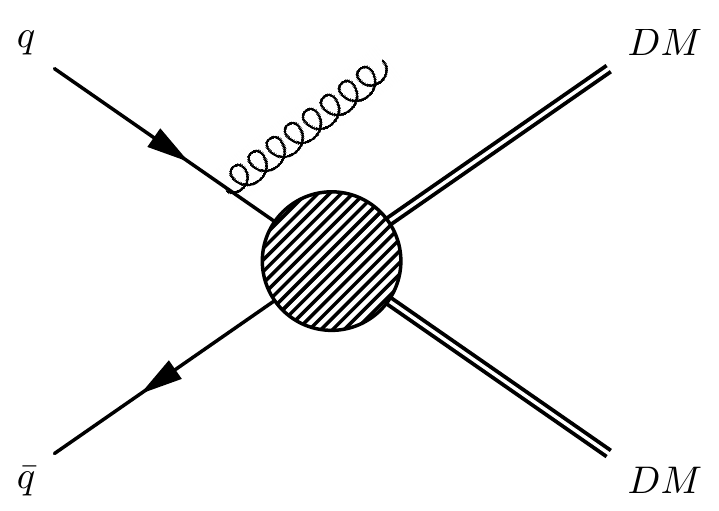
\includegraphics[width=.4\textwidth]{monojet.png} 
 \caption{Illustration of EFT dark matter production in the monojet final state.}
 \label{fig:monojet_diagram}
\end{figure}

In the two dark matter searches covered in this thesis, the results have been interpreted in terms of simplified models. The monojet search described in Chapter~\ref{ch:monojet} includes several simplified models recommended by the dark matter forum. Four types of mediators are considered, i.e. a vector, axial, scalar, and pseudoscalar mediator. In the case of a scalar or pseudoscalar coupling, the production mode is dominated by gluon fusion. As illustrated in the right diagram of Figure~\ref{fig:monojet_diagrams}, the scalar is produced through a $t$ or $b$ quark loop. A Yukawa coupling is assumed for the coupling of the mediator to Standard Model particles, proportional to the mass of the particle. For a vector or axial mediator, the production happens through the fusion of two quarks into a heavy mediator, similarly to the $Z$ and $W$ boson production. The coupling to quarks and potentially leptons is taken to be unity, and universal for all flavours. For all mediator types, the coupling to the dark matter particles is assumed to be unity. In addition, the minimal width assumption is made, implying that the mediator couples to all Standard Model and the dark matter particle and no extra particles are introduced. If such particles would be present, the width would increase and the sensitivity of the analysis would be reduced. A scan is then performed over the mass of the dark matter candidate and the mass of the mediator.

\begin{figure}[ht]
  \centering
 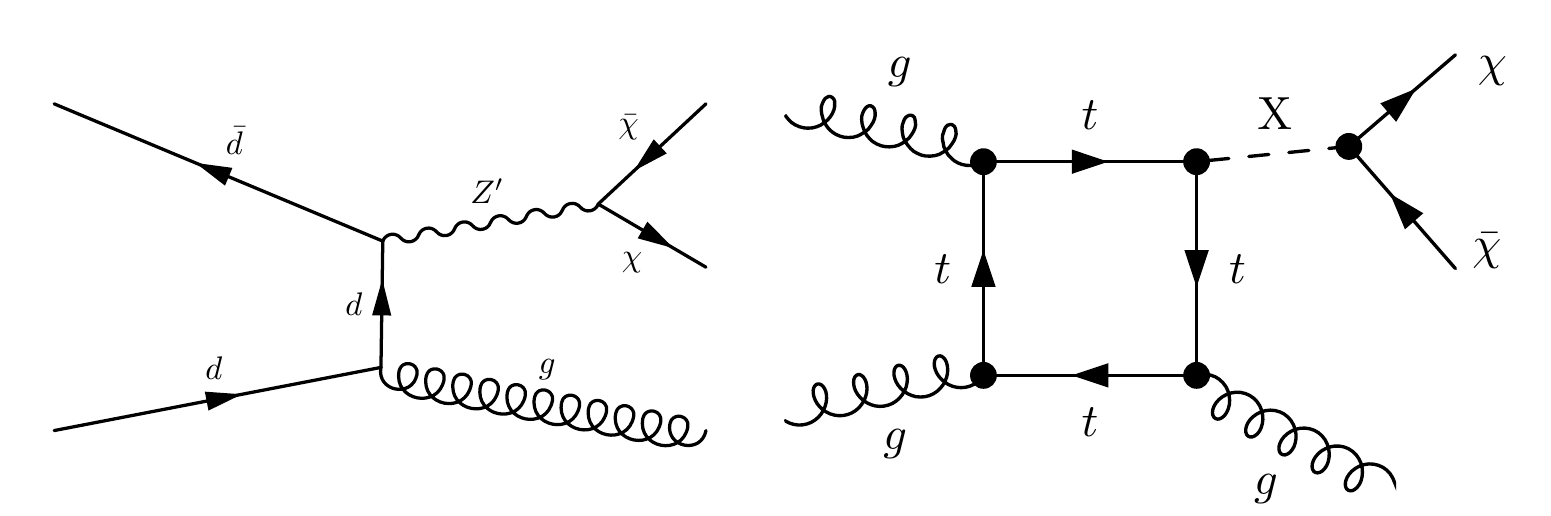
\includegraphics[width=.9\textwidth]{monojet_simplifiedmodel.png} 
 \caption{The vector (left) and scalar (right) production diagrams in the monojet final state.}
 \label{fig:monojet_diagrams}
\end{figure}

Furthermore, some non-standard dark matter models are investigated as well in the monojet analysis, namely a complete simplified scalar model, known as the inert two Higgs doublet model and a baryon number violating dark matter model which can explain electroweak baryogenesis~\cite{}, known as non-thermal dark matter. In contrast to the simplified models, these theories are completed theories. The first consists of an extended scalar field theory, while the second consists of resonant production induced by flavour changing neutral currents.

The \acs{SIMP} simplified model on which the trackless jets analysis detailed in Chapter~\ref{ch:SIMPs} is a specific simplified model which is not part of the models recommended by the dark matter forum. It is described in more detail in Section~\ref{sec:SIMP}.

\section{Strongly Interacting Massive Particles}
\label{sec:SIMP}

As no observation of dark matter has been made so far, despite many searches probing the more popular models described in the previous section, many scenarios now venture beyond minimal models or give up basic assumptions for the \ac{WIMP}. In the following model, which is studied in this thesis, the interaction cross section of the dark matter with normal matter is so high that the particles are no longer \acp{WIMP}, but so-called \acp{SIMP}. This model can also be motivated by the long lasting interest for \ac{SIDM}\footnote{Incidentally, self-interacting and strongly interacting share the same abbreviation, such that SIDM can also stand for strongly interacting dark matter and SIMP for self-interacting massive particles in the literature.} particles with a large cross section~\cite{Spergel:1999mh}, which could help to explain observations that present a challenge for the cold dark matter scenarios, such as the missing satellites or core-cusp problems~\cite{Bullock:2010uy,BoylanKolchin:2011de, Weinberg:2013aya,Famaey:2013ty}. While it is possible to create models with a strongly interacting hidden sector that is weakly coupled to the Standard Model particles, \ac{SIDM} particles that interact rather strongly with the known matter particles can be considered as well.

\subsection{The SIMP simplified model}

In this simplified model, the dark matter particles $\chi$ can be produced at the \ac{LHC} in pairs, through a new strong interaction with a new mediator $\phi$, as illustrated in Figure~\ref{fig:diagram}. These \acp{SIMP} are neutral and stable, and are generated off-shell as the mediator is very light, of the order of the pion mass: $m_{\phi} = 140$~MeV. We only consider the case of fermionic candidates, since the bosonic form is ruled out by constraints coming from neutron stars and black holes, as is described in Section~\ref{sec:SIMP_constraints}. Both the cases with a scalar or a vector mediator can be studied, and the corresponding interaction Lagrangian is
\begin{equation} \label{eq:SIMP_lagrangian}
 \mathcal{L}_{\mathrm{int}} = 
 \begin{cases}
  -g_{\chi}\phi\bar{\chi}\chi - g_q\phi\bar{q}q & \text{(scalar mediator)}\\
  -\tilde{g}_{\chi}\phi_{\mu}\bar{\chi}\gamma^{\mu}\chi - \tilde{g}_q\phi_{\mu}\bar{q}\gamma^{\mu}q & \text{(vector mediator)}
 \end{cases}
\end{equation}
with $g_{\chi}g_q,\tilde{g}_{\chi}\tilde{g}_q <0$ to avoid the formation of bound states. For simplicity we assume that the \acp{SIMP} have a universal coupling to quarks, although a flavour dependent coupling could be preferred, as light \acp{SIMP} with a significant coupling to $b$ or $c$ quarks are probably constrained by B and D meson phenomenology. \acp{SIMP} lighter than about 5~GeV could for example appear in the decay of $b$ or $c$ quarks, and would be constrained by limits on the invisible decay of B and D mesons.

\begin{figure}[ht]
  \centering
  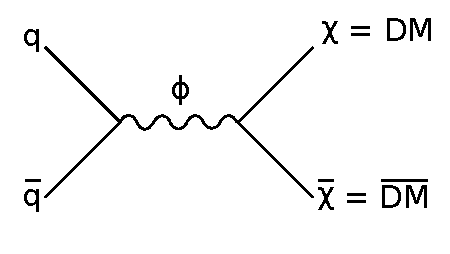
\includegraphics[width=0.45\textwidth]{diagram.pdf}\hfill%
  \caption{Feynman diagram showing the production of a SIMP pair, through a new low-mass mediator.}
  \label{fig:diagram}
\end{figure}

Introducing a new strong interaction between quarks can however modify nuclear potentials. In order to keep the impact small, the mediator is assumed to not modify nuclear potentials by more than $\mathcal{O}(10\%)$, such that $g_{\chi N} \lesssim 0.3g_{\pi NN}\sim 3$ for a mediator with the mass of a pion, where $g_{\pi NN} \sim 13$ is the effective pseudoscalar pion-nucleon coupling~\cite{Donoghue:1992dd}. The quoted values are however not very precise, as a large spread of values can be found in the literature for meson-nucleon effective couplings, sometimes differing by a factor 2 or more (see e.g.~\cite{Downum:2006re} for comparison). This shows the difficulty of dealing with strong interactions in the framework of effective field theories, which arise because contributions from many mesons need to be taken into account, each of them with a different coupling. No constraints on modified strong interactions at low energies seem to exist in literature so far, however searches at fixed-target experiments do place constraints on the existence of strongly interacting stable neutral particles.

In summary, the model has 4 free parameters: the two couplings, the mass of the mediator $m_{\phi}$, and the mass of the \ac{SIMP} $m_{\chi}$. At the \ac{LHC}, only the product of the couplings appears, while astrophysical observations constrain both the dark matter self-interaction and the interaction with the Standard Model.

\subsection{Experimental constraints}
\label{sec:SIMP_constraints}

Naively, one would expect such an unusual model with strong interactions not to be viable, as various types of experiments and observations set constraints on \acp{SIMP} as dark matter candidates. However, some of these limitations can be avoided by the assumptions in the model described above. The relevant existing measurements are described below, showing there is a still a part of phase space which remained unexplored so far.

\begin{itemize}
 \item[] \textbf{Bound states}\\
Searches for heavy isotopes, in particular heavy water, constrain the formation of bound states between \acp{SIMP} and nucleons, ruling out particles with a mass below 10~TeV for the scenario with \acp{SIMP} as dominant contribution to dark matter. This constraint is evaded by assuming a purely repulsive \ac{SIMP}-nucleon interaction with opposite sign couplings, as is specified in the Lagrangian~(\ref{eq:SIMP_lagrangian}). In the vector mediator case, vector mediators would however couple to the dark matter antiparticles with an opposite charge. This is avoided if no dark matter antiparticles are around, i.e. if the abundance of dark matter is asymmetric. A reason for having asymmetric \acp{SIMP} is that if they are the dominant source of dark matter, then the dark matter abundance is set by either an asymmetry or through a non-thermal mechanism. In the case of a symmetric \ac{SIMP} candidate, the dark matter abundance is determined by thermal freeze-out, and it can only be a sub-dominant component. Additional constraints also exist on the dark matter self-interacting strength from halo shapes and merging galaxies such as the Bullet cluster~\cite{Randall:2007ph, Feng:2010gw}.
% EB: this is a rather dense paragraph that might benefit from a bit more explanation

\item[] \textbf{Earth heating}\\
A second argument for an asymmetric abundance of \acp{SIMP} comes from experiments measuring the heat emitted from the Earth's core. For the typical \acp{SIMP} cross sections, the dark matter particles can be captured by the Earth and accumulate in its core over time. Annihilating \acp{SIMP} would then provide a substantial source of heat and could modify the Earth's heat flow. This can be measured by detectors in deep underground shafts~\cite{Mack:2007xj} and rules out the scenario with symmetric \acp{SIMP}.

\item[] \textbf{Neutron stars and black holes}\\
In the asymmetric scenario, light scalar dark matter particles can however be collected in the cores of neutron stars and cause them to collapse into black holes. Bosonic dark matter candidates are therefore excluded, and we consider only fermionic candidates as mentioned previously.

\item[] \textbf{Direct detection searches}\\
Many bounds on the \ac{SIMP} parameter space also come from the direct detection searches. Underground experiments, such as CDMS and XENON,
% EB: reference?
place strong constraints at smaller cross sections, about 5 orders of magnitude below the \ac{SIMP} cross section, as can be seen from Figure~\ref{fig:SIMP_summary}. At the higher cross sections considered here, the \acp{SIMP} are stopped by the Earth's atmosphere, and they cannot reach the underground detectors. At higher altitudes however, space or airborne experiments such as RSS~\cite{Rich:1987st}, a balloon-based experiment with a silicon semiconductor detector, and XQC~\cite{Erickcek:2007jv}, a sounding rocket experiment, exclude \acp{SIMP} in some regions of phase space. More details on these constraints can be found in~\cite{Mack:2007xj}, where they have been extensively reviewed.

\item[] \textbf{Nucleosynthesis and cosmic rays}\\
There are also bounds from primordial nucleosynthesis and cosmic rays, reviewed in \cite{Mack:2012ju} and \cite{Cyburt:2002uw}. The protons in cosmic rays can scatter off dark matter particles and create neutral pions, which decay to photons and could be detected in gamma ray telescopes. Although limits have been placed on dark matter-nucleon interactions~\cite{Cyburt:2002uw}, these constraints depend on many assumptions and adopt a form of the dark matter density near the galactic core. Since the considered model describes a nonstandard form of dark matter with a relatively strong interaction with baryons, these densities may be considerably different.

\item[] \textbf{\ac{CMB} and large scale structure}\\
Observations of the \ac{CMB} anisotropies and the large scale structure power spectrum, including from the Lyman-$\alpha$ data~\cite{Chen:2002yh,Dvorkin:2013cea} additionally also place strong constraints on interactions between dark matter and baryons.

\item[] \textbf{Fixed-target experiments}\\
Finally, a relatively old fixed-target experiment led in 1976 at FNAL with a beam of neutral particles produced by 300~GeV protons hitting a beryllium target was used to look for massive, strongly interacting, neutral particles~\cite{Gustafson:1976hd}. The mass of the particles was determined using their flight time and their kinetic energy which was measured in a calorimeter. Neutral particles with a mass larger than 2~GeV were searched for, in order to discriminate the candidates from the background of neutrons and lighter hadronic states, up to $m_{\chi} \lesssim \sqrt{E/2} \approx 12$~GeV, limited by the beam energy of $E = 300$~GeV. Single particle production was considered, but the results apply to pair production as well when they are translated into the case where 2 neutral particles are boosted and fly away in the same direction. 
The search showed no significant excess above the expected background and limits were placed on the invariant production cross section per nucleon versus the neutral particle interaction cross section. As an example, for an interaction cross section of 1~mb, a limit on the total production cross section of about $2.5\times10^{-35}\ \mathrm{cm}^2 = 25$~pb is found, and this  limit is reported by the Particle Data Group~\cite{Agashe:2014kda}. Comparing the considered \ac{SIMP} model to this result by simulating the pair production at $\sqrt{s} = 25$~GeV, one can conclude that \acp{SIMP} between 2 and about 6~GeV are already excluded by this experiment~\cite{Daci:2015hca}.

\begin{figure}[ht]
  \centering
  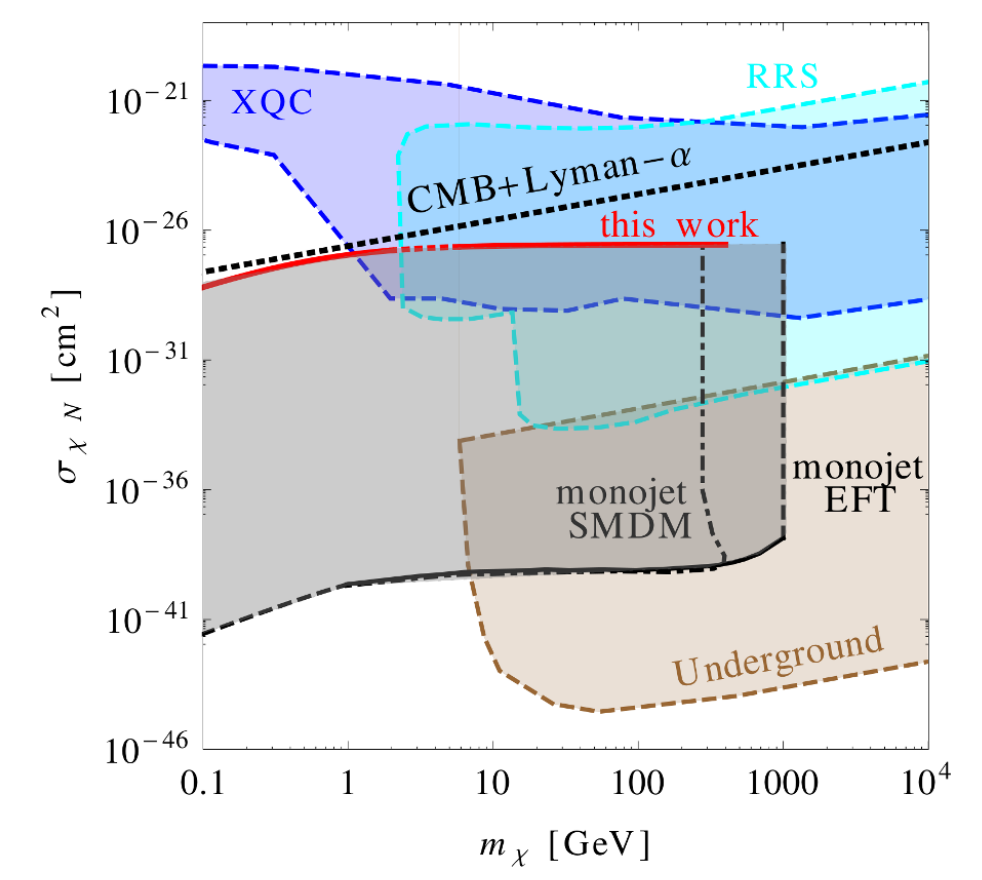
\includegraphics[width=0.8\textwidth]{SIMP_summary.png}\hfill%
  \caption{Summary plot showing the \ac{SIMP} model (red) in comparison with the most important applicable constraints, coming from the LHC monojet analyses (black), the atmospheric XQC and RRS experiments (blue), underground experiments (brown), and the \ac{CMB} observations and Lyman-$\alpha$ data (black dashed line). Figure taken from~\cite{Daci:2015hca}.}
  \label{fig:SIMP_summary}
\end{figure}

\end{itemize}

\clearpage{\pagestyle{empty}\cleardoublepage}

\graphicspath{{chapt_dutch/}{intro/}{detector/}}

% Header
\renewcommand\evenpagerightmark{{\scshape\small Chapter 3}}
\renewcommand\oddpageleftmark{{\scshape\small The LHC and the CMS Detector}}

\hyphenation{}

\chapter{The LHC and the CMS Detector}
\label{ch3}

In order to investigate the currently unsolved mysteries of particle physics, such as the existence of dark matter, many experiments can be conducted, among other things at particle colliders. The largest particle accelerator in the world is the \ac{LHC}, located at the \ac{CERN} in Geneva, Switzerland. At this accelerator, protons are being accelerated at energies up to \SI{6.5}{TeV}, giving rise to a record center-of-mass energy of \SI{13}{TeV} in the proton collisions. Using data from the collisions generated at the interaction points along the accelerator ring, the Standard Model can be tested in many ways and searches for particles beyond the Standard Model can be performed. 

In Section~\ref{sec:lhc} more details are given about the \ac{LHC} and the 4 main experiments situated at the interaction points. In particular, the general-purpose \ac{CMS} detector is described in Section~\ref{sec:CMS}.

\section{The Large Hadron Collider at CERN} 
\label{sec:lhc}

The \ac{LHC} was built in the already existing \ac{LEP} collider tunnel, which was excavated in the 1980's and has a circumference of 27.6~km. Contrary to the \ac{LEP} collider, the \ac{LHC} accelerates particles of the same charge, namely protons or lead ions. Much higher luminosities can therefore be reached, since only particles are used and the generation of antiparticles is not needed. This was the limiting factor at the Tevatron, where protons and antiprotons were used. Additionally, at the probed energies the colliding particles are not the protons or ions, but their constituents, which carry a varying fraction of the total momentum. %and thus cover a wide energy range. 
%This is in contrast to electron-positron colliders such as the \ac{LEP} collider, where the energy is fixed, which 
This makes the \ac{LHC} an ideal instrument for exploration at higher energies, as the collisions naturally cover a wide energy range.

\subsection{The LHC injector chain}

The protons (or lead ions) can not directly be injected in the \ac{LHC}, but need to be accelerated gradually in several pre-accelerators, as illustrated in Figure~\ref{fig:accelerators}. For the proton beams, the \ac{LHC} injection chain starts at a bottle of hydrogen, where protons are stripped from the hydrogen atoms and accelerated up to \SI{50}{MeV} by a linear accelerator (LINAC2). The protons are then transfered to a chain of circular accelerators, starting with the \ac{PSB} which accelerates them to an energy of \SI{1.4}{GeV}. Next, the protons go through the \ac{PS} and are delivered to the \ac{SPS} at an energy of \SI{26}{GeV}. Finally, the protons are injected in the \ac{LHC} in opposite direction with an energy of \SI{450}{GeV}. 
% In the \ac{LHC} the protons are then accelerated to \SI{3.5}{TeV} (in 2010 and 2011) or \SI{4}{TeV} (in 2012) during Run 1, and to \SI{6.5}{TeV} during Run 2 (since 2015).

The lead ions are first accelerated in a different linear accelerator, LINAC3, before being injected in the \ac{LEIR} at an energy of \SI{4.5}{MeV} per nucleon. Here the ions are accelerated to an energy of \SI{72}{MeV} per nucleon, and they then follow the same path as the protons through the \ac{PS}, where they are accelerated to \SI{5.9}{GeV} and stripped from the last of their electrons, and the \ac{SPS}, where they are accelerated to \SI{177}{GeV}. The record center-of-mass energy for heavy ion collisions at the \ac{LHC} so far has been \SI{5.02}{TeV} and \SI{8.16}{TeV}, for lead-lead (Pb-Pb) and proton-lead (p-Pb) collisions in 2015 and 2016, respectively.

\begin{figure}[ht]
  \centering
 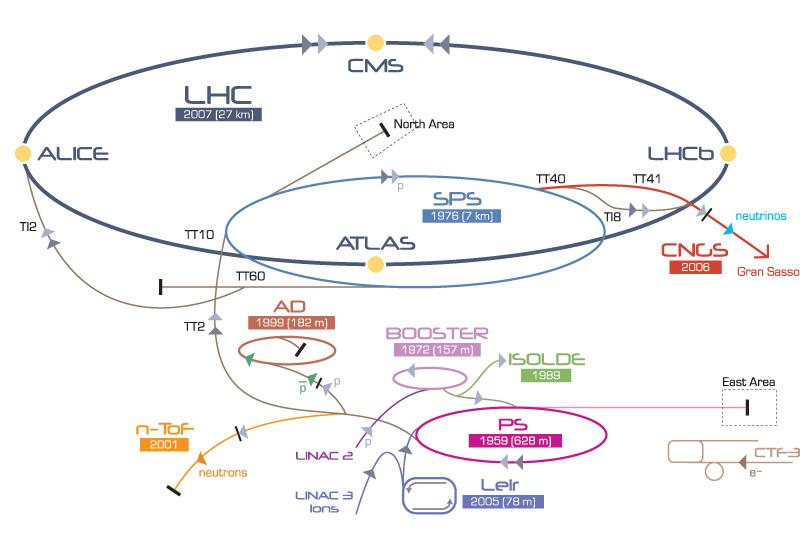
\includegraphics[width=.75\textwidth]{lhc_complex}
 \caption{Schematic view of the various linear and circular accelerators of the \ac{CERN} accelerator complex, including the \ac{LHC} injection chain.}
 \label{fig:accelerators}
\end{figure}

\subsection{The Large Hadron Collider}

The most relevant specifications for a particle physics accelerator are the maximum energy and the luminosity that can be reached. High energy is necessary in order to be able to create new heavy particles, which are for example predicted in many theories beyond the Standard Model.

The protons are kept on the correct orbit by the 1232 \ac{LHC} dipole magnets. These magnets are cooled down to 1.9 K with liquid Helium and supplied with a current of 12~kA to reach the design field of 8.33~T. This limits the maximum beam momentum of the accelerator to 
\begin{equation}
 p = B/\rho = 8.33\, \mathrm{T}/2804\,\mathrm{m}=7\,\mathrm{TeV/c},
\end{equation}
with $\rho$ the bending radius of the tunnel. The protons are accelerated up to the desired energy by \ac{RF} cavities, which produce an oscillating electric field. 
%As a consequence, late or early protons will feel a stronger or weaker acceleration, respectively.

A high event rate or luminosity~$\mathcal{L}$ is equally important, to obtain a sufficiently high number of collisions. For a process with cross section $\sigma$, this rate is 
\begin{equation}
 \frac{dN}{dt} = \mathcal{L}\sigma .
\end{equation}
In order to achieve the high design luminosity of $10^{34}$ cm$^{-2}$s$^{-1}$ in the \ac{LHC}, the protons are concentrated in bunches with a \SI{25}{ns} spacing, which are focused by strong quadrupole magnets around the interaction regions. Additionally, 2\SI{25}{ns} gaps are present as well between the bunch trains, corresponding to the rise time of the injection kicker magnets. One gap of 3~$\mu$s is necessary as well to allow clean beam dumps. These requirements limit the number of bunches to a maximum of 2808.

% Additionally, over 8000 higher-order multipole and corrector magnets focus and stabilize the proton beams.

After almost 25 years of design and construction, the \ac{LHC} was completed in 2008 and the commissioning of the machine started. However, during a powering test on 19 September of the same year an electric arc developed inside a bus bar which led to a large release of helium and a pressure wave that caused extensive mechanical damage to the affected LHC sector. This incident delayed the first collisions, with one bunch per beam and at a beam energy of \SI{900}{GeV}, until late 2009. During 2010 and 2011 a center-of-mass energy of \SI{7}{TeV} was used for the collisions, which was then increased to \SI{8}{TeV} in 2012. The instantaneous luminosity was also increased, starting from $2 \times 10^{32}$ cm$^{-2}$s$^{-1}$ in 2010 to more than $6 \times 10^{33}$ cm$^{-2}$s$^{-1}$ in 2012. During the 3 years of data-taking in Run~1, data corresponding to an integrated luminosity of 45.0~pb$^{-1}$, 6.1~fb$^{-1}$, and 23.3~fb$^{-1}$, respectively, were delivered. After Run~1, a long shutdown (LS1) of 2 years followed, which was used to correct the problems that were discovered in the aftermath of the incident at the startup in 2008, and to upgrade and consolidate the experiments located on the \ac{LHC} ring.

In 2015, the \ac{LHC} restarted operations with Run~2, at an even higher center-of-mass energy of \SI{13}{TeV}. During 2016 the design luminosity of $10^{34}$ cm$^{-2}$s$^{-1}$ was exceeded and a total of 41~fb$^{-1}$ of data were delivered. A comparison of the delivered integrated luminosity per year is shown in Figure~\ref{fig:lumi}.

\begin{figure}[ht]
  \centering
 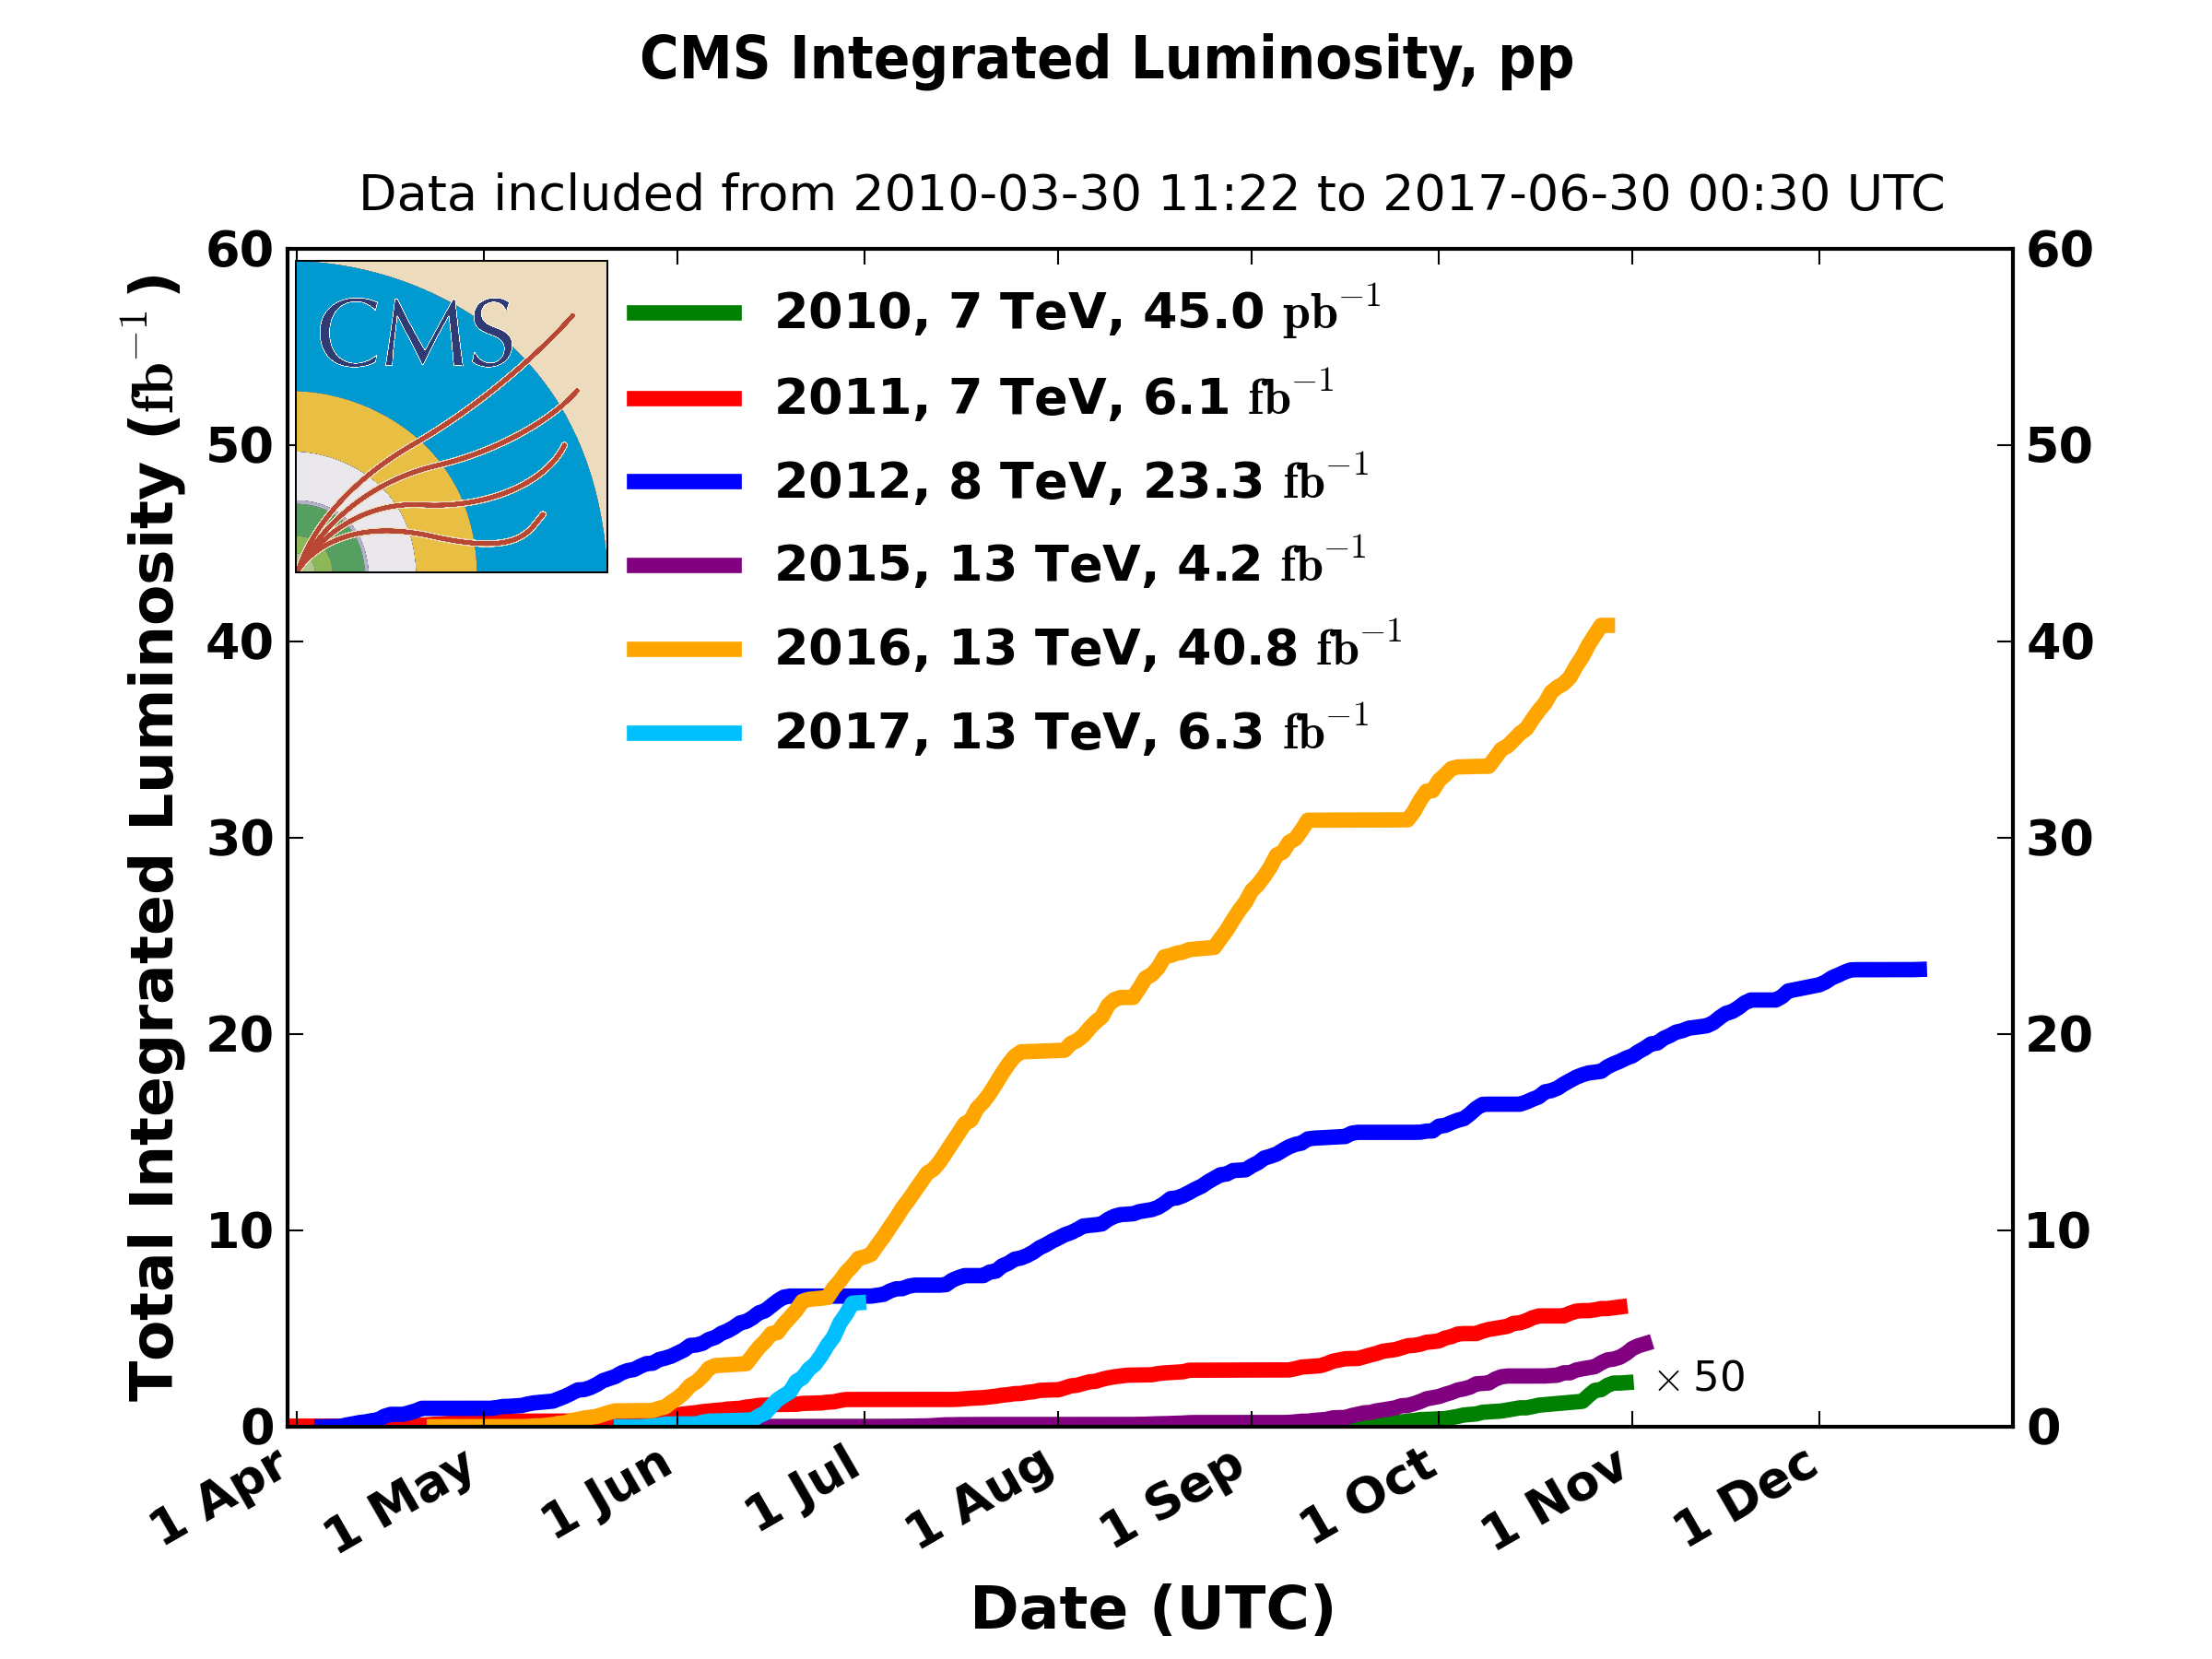
\includegraphics[width=.75\textwidth]{CMS_lumi_allyears}
 \caption{Overview of the integrated luminosity delivered to the CMS detector during Run~1 (2010 to 2012) and Run 2 (2015 to 2017).}
 \label{fig:lumi}
\end{figure}

\subsection{The experiments at the LHC}

There are four \acp{IP} where the proton or lead ion beams of the \ac{LHC} can collide, and around each of these points large particle detectors were built in order to record the generated collisions. The \acs{ATLAS} and \ac{CMS} detectors, located at \ac{IP}1 and \ac{IP}5, are both high luminosity general-purpose detectors and consist of several layers surrounding the \ac{IP} in an onion-like structure to avoid particles escaping detection. These detectors can cover a wide range of high energy physics, from precision measurements of the Standard Model to searches beyond the Standard Model. At \ac{IP}2 the \acs{ALICE} detector is specialized in heavy ion collisions with low instantaneous luminosities, around $10^{27}$cm$^{-2}$s$^{-1}$. With this detector information is gathered about the quark-gluon plasma, a state of matter that exists at extremely high temperatures and densities where quarks and gluons are no longer confined in hadrons. The fourth main detector, \acs{LHCb}, is located at \ac{IP}8 and requires instantaneous luminosities of the order of a few $10^{32}$cm$^{-2}$s$^{-1}$. Using this detector $b$ quarks are being studied, focusing among other things on the matter-antimatter asymmetry in the universe.

\section{The CMS detector} 
\label{sec:CMS}

The searches described in this thesis were conducted using data collected with the \ac{CMS} detector, a general-purpose detector located on the \ac{LHC} ring. It consists of the typical components of a particle physics detector, namely a tracker, an \ac{ECAL}, a \ac{HCAL}, a solenoidal magnet, and muon detectors. One peculiar aspect is however that both calorimeters are situated inside the superconducting magnet. This design was chosen in order to improve the energy resolution by reducing the amount of material in front of the calorimeters. The overall detector has a length of 21.6 m, a diameter of 14.6 m and a total weight of 12500 t. A schematic overview is shown in Figure~\ref{fig:CMS}.

\begin{figure}[ht]
  \centering
 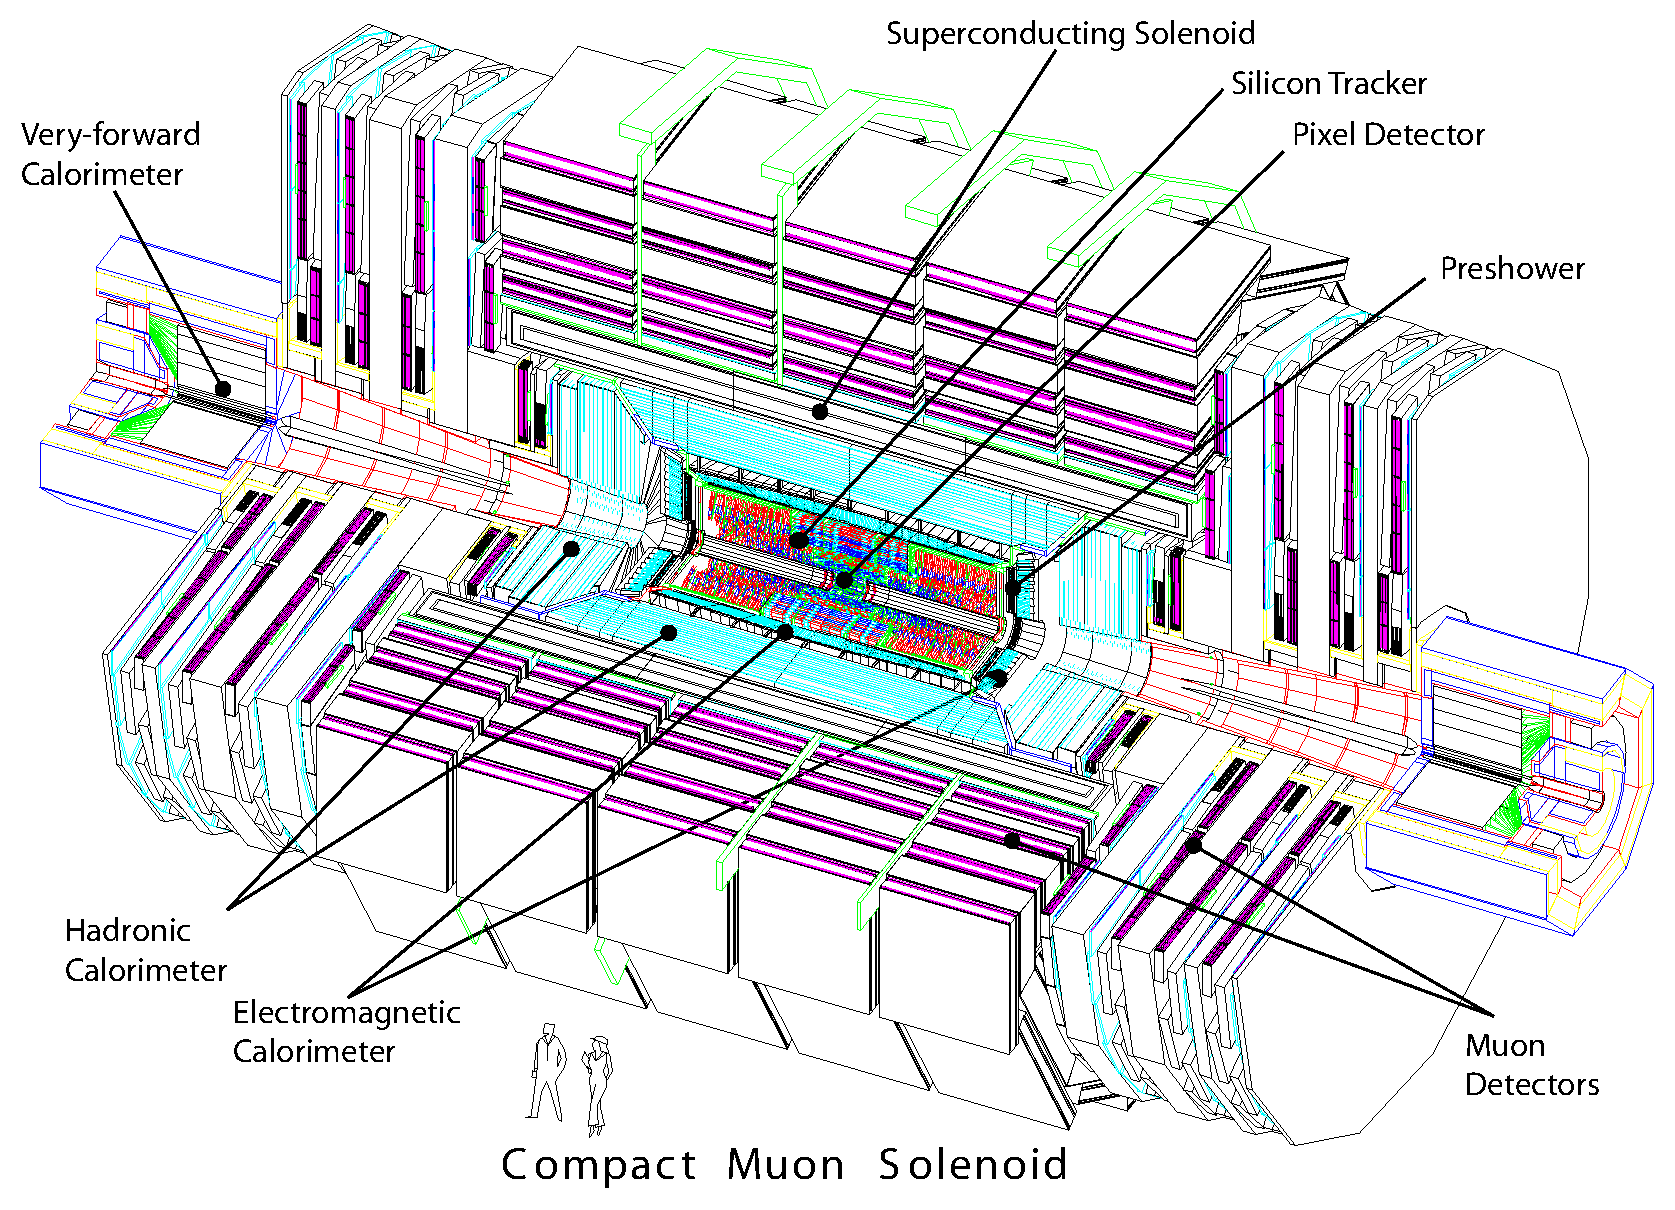
\includegraphics[width=.9\textwidth]{cms_complete_labelled}
 \caption{The \ac{CMS} detector, consisting of the pixel and strip tracker, the \protect\acf{ECAL} with preshower, the \protect\acf{HCAL} with its forward component, and the muon systems.}
 \label{fig:CMS}
\end{figure}

The CMS coordinate system places the origin at the nominal collision point. The $x$ axis is perpendicular to the beam and points towards the center of the \ac{LHC} ring, the $y$ axis is vertical and pointing upwards, and the $z$ axis is defined anticlockwise along the beam direction. The azimuthal angle $\phi$ is then defined in the $xy$ plane, relative the the $x$ axis and the polar angle $\theta$ is measured with respect to the $z$ axis. In general, the polar angle is converted into the pseudorapidity
\begin{equation}
 \eta = -\ln\left(\tan\frac{\theta}{2}\right)
\end{equation}
for convenience, since differences in pseudorapidity are invariant under Lorentz boosts along the $z$ axis. A pseudorapidity of 0 corresponds to the direction perpendicular to the beam ($\theta = \pi/2$), and an infinite pseudorapidity corresponds to the direction parallel to the beam ($\theta = 0$).

Due to the conservation of momentum before and after the collision, the momenta of the particles in the final state of a collision should be balanced in the transverse plane. Another variable that is therefore often used in particle physics is the transverse momentum of a particle, defined as 
%the momentum component in the $xy$ plane:
\begin{equation}
p_T = p \cdot \sin \theta .
\end{equation}

\subsection{The tracker}

The innermost part of the \ac{CMS} detector, closest to the \ac{IP}, is the tracking system, which is designed to provide a precise measurement of the trajectories of charged particles. This all-silicon detector is divided into a pixel and a strip detector, with a layout as shown in Figure~\ref{fig:cmstracker}. The inner part, consisting of pixel modules, provides very precise 3D hits, which are important for vertex reconstruction and track seeding. This allows to have a precise measurement of secondary vertices and track impact parameters, necessary for the efficient identification of e.g. heavy flavor particles. As the hit occupancy is lower in the outer part of the detector, a larger cell size can be afforded, and silicon strips are used instead of pixels. This strip detector provides a large lever arm and a link to the calorimeters and the muon system. The tracker covers a pseudorapidity range $|\eta| < 2.5$.

\begin{figure}[ht]
  \centering
 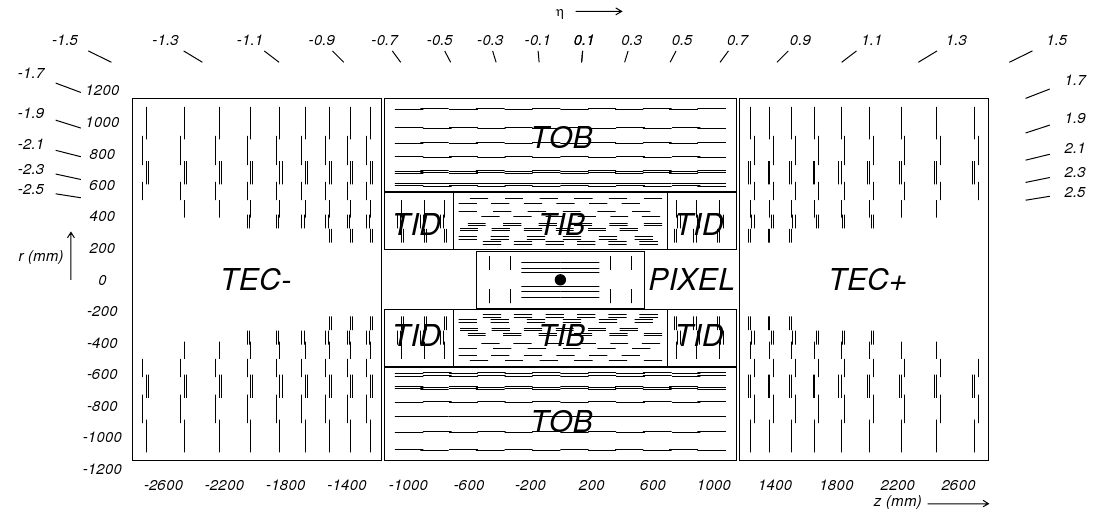
\includegraphics[width=.9\textwidth]{fig_cmstracker}
 \caption{A transverse view of the pixel and strip tracker detectors.}
 \label{fig:cmstracker}
\end{figure}

\subsubsection{The pixel tracker} 

The pixel tracker was replaced during the extended technical stop in 2016 and 2017~\cite{CMS:2012sda}, as a part of the \ac{CMS} Phase 1 upgrades. As the data used for this thesis were recorded before that, only the so-called Phase 0 detector is described here. 

For the pixel modules n+ pixels on n-substrate are used, allowing the sensors to also work in under-depletion after type inversion. The 1440 modules are arranged in several cylindrical layers and disks, as illustrated in Figure~\ref{fig:cmstracker}. The barrel, consisting of 3 pixel layers surrounding the beam pipe at radii of 4.4, 7.3 and 10.2~cm, is complemented by the forward pixel detector, composed of 2 endcap disks on each side extending from 6 to 15~cm in radius. The barrel and the forward parts contain respectively 48 million and 18 million pixels with a size of $100 \times 150\ \mu\mathrm{m}^2$, covering a total area of 1.06~m$^2$.

In the barrel, the magnetic field of CMS is perpendicular to the drift of the electrons to the collecting pixels, which results in a Lorentz drift. This drift leads to a spread of the charge over several pixels. Since the read-out of the modules is analog, an improved spatial resolution can therefore be achieved with charge interpolation. In the forward pixel detector the drift of the electrons would be parallel to the magnetic field so in order to profit from the Lorentz angle, the modules are tilted by 20\degree in a turbine-like arrangement, as can be seen in Figure~\ref{fig:pix}. A spatial resolution of 10 $\mu$m (30 $\mu$m) can be achieved in the local directions $x$ ($y$) of the module, respectively. In the barrel $x$ is the longitudinal direction perpendicular the the beam and $y$ is the longitudinal direction parallel to the beam. 
%The resolution will degrade with radiation damage, since the charge-sharing will be reduced by a decrease in depletion depth or an increase of bias voltage.

\begin{figure}[ht]
  \centering
 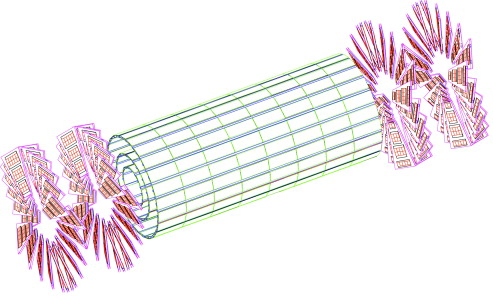
\includegraphics[width=.6\textwidth]{pixel}
 \caption{A 3D view of the barrel and forward pixel detector.}
 \label{fig:pix}
\end{figure}

The signals from the pixel sensors are read out by custom \acp{ROC}, which amplify and store the signals, and already apply zero-suppression on-detector. The data rate from the detector to the \acp{FED} is therefore not constant for every event. Additionally, if there are too many hits on a pixel module for a given event, they can not all be stored on the finite buffer of the \ac{ROC}. Consequently, as the instantaneous luminosity increases the pixel modules start to show a ``dynamic inefficiency''  which is most pronounced in the first layer, closest to the beampipe. This was one of the main motivations for the Phase 1 upgrade of the pixel detector.

\subsubsection{The strip tracker}

The outer part of the tracker consists of 15~148 strip modules, which are distributed among multiple barrel layers and endcap disks and make up a total active area of 198 m$^2$. The inner part is composed of 4 \ac{TIB} layers with 3 \ac{TID} on each side. Surrounding these are 6 \ac{TOB} layers and the 2 \ac{TEC}, which are composed of 9 disks. This geometric arrangement is shown in Figure~\ref{fig:cmstracker}, with double lines to indicate back-to-back modules. These so-called double-sided modules are mounted with a stereo angle of 100 mrad to improve the 3D point resolution by providing a measurement of the $z$ and $r$ coordinate in the barrel and disks, respectively. The choice of strip pitches is driven by the two particle separation capability and two-hit resolution, and ranges from \SI{80}{\micro m} to \SI{205}{\micro m}. The length of the strips varies from \SI{63}{mm} to \SI{117}{mm}, minimizing the occupancy and noise levels.

In the \ac{TOB} and the 3 outermost rings of the \ac{TEC} two silicon sensors are daisy chained, while single sensors are used in the inner part. This is done to limit the number of read-out channels, since the area that had to be instrumented is larger in the outer region. The larger cell size can be afforded  due to the lower occupancy in the outer part. However, the noise of the sensors also increases with strip length, so thicker silicon sensors, 500 $\mu$m compared to 320$\mu$m in the inner part, are used in order to collect more signal per traversing particle.

The strip sensors are single sided p-on-n type silicon. The signals from the sensors are amplified, shaped, and stored by 4 or 6 custom APV25 chips per module. When the trigger has made a positive decision, the analog signals from two APV25 chips are multiplexed and sent to the \ac{FED} boards in the service cavern via optical fibers, where they are converted to digital signals. The \acp{FED} then perform pedestal and common mode subtraction as well as cluster finding. Additionally, the data is sparsified in these off-detector electronics, before being sent to the CMS central \ac{DAQ}. Due to charge sharing, this analog read-out scheme also results in an improved spatial resolution of 15 to 40 $\mu$m, depending on the position of the modules and the strip pitch. 

%Different strip pitch/width because 80 - 205 µm depending on the sensor type
% 
% \subsubsection{Tracking}
% 
% The tracks of charged particles going through the \ac{CMS} tracker are reconstructed with an iterative tracking approach. This is used to cope with the high occupancy and consequently high combinatorics. Additionally, the first iterations search for tracks with less possible combinations, such as tracks with many pixel hits or a high momentum. After every iteration, the hits associated with the found track are removed to reduce the combinatorics. Each iteration consists of four steps:
% \begin{enumerate}
%  \item \textbf{Seed generation.} In this first step hits are combined into seeds for the subsequent track finding. In the initial iterations pixel triplets are used, then pixel pairs, in order to take gaps or non-working modules into account. Next, mixed pixel/strip triplets are taken, and finally strip-only seeds are used. These additional iterations improve the acceptance in $p_T$ and in displacement with respect to the primary vertex.
%  \item \textbf{Track finding}. The seeds are used as starting point for a Kalman filter algorithm. This method extrapolates the seed trajectory outward to the next layer, taking into account potential energy loss and multiple scattering. If compatible hits are found in the next layer, the parameters of the trajectory are updated. This process continues until the outermost layer of the tracking system. Using this method, a given seed can generate multiple tracks, or different tracks can share hits. A trajectory cleaner therefore determines the fraction of hits the tracks have in common and discards the track with the lowest number of hits when there are too many shared hits. If both tracks have the same number of hits, the track with the largest $\chi^2$ value is removed.
%  \item \textbf{Track fitting.} The track parameters are then refitted using a Kalman filter and smoother, taking all hits determined in the track finding step into account.
%  \item \textbf{Track selection.} Finally, the tracks are selected based on quality requirements, such as the number of layers that have hits, the $\chi^2/$dof, and the distance to a primary vertex. This greatly reduces the fraction of reconstructed tracks that are fake.
% \end{enumerate}
% 
% The performance of the track reconstruction is excellent, and a high track-finding efficiency is obtained~\cite{Chatrchyan:2014fea} while keeping the rate of fake tracks negligible. The highest tracking efficiency is obtained for muons, which traverse the full detector volume and have an improved momentum resolution due to tracking information from the muon detectors giving a long lever arm. For isolated muons with $p_T$ between 1 and \SI{100}{GeV} the tracking efficiency is higher than 99\% for the entire $\eta$ coverage of the tracker, as can be seen from the left plot in Figure~\ref{fig:eff_eta}. The $p_T$ resolution is about 2-3\% for a muon with $p_T = $ \SI{100}{GeV} up to $|\eta| < 1.6$, but worsens for higher pseudorapidities. Different types of particles interact differently with the detector material. Charged hadrons, for example, are also subject to elastic and inelastic nuclear interactions and have a tracking efficiency of 80-95\% depending on pseudorapidity and transverse momentum, as shown in the right plot of Figure~\ref{fig:eff_eta}.
% 
% \begin{figure}[ht]
%   \centering
% 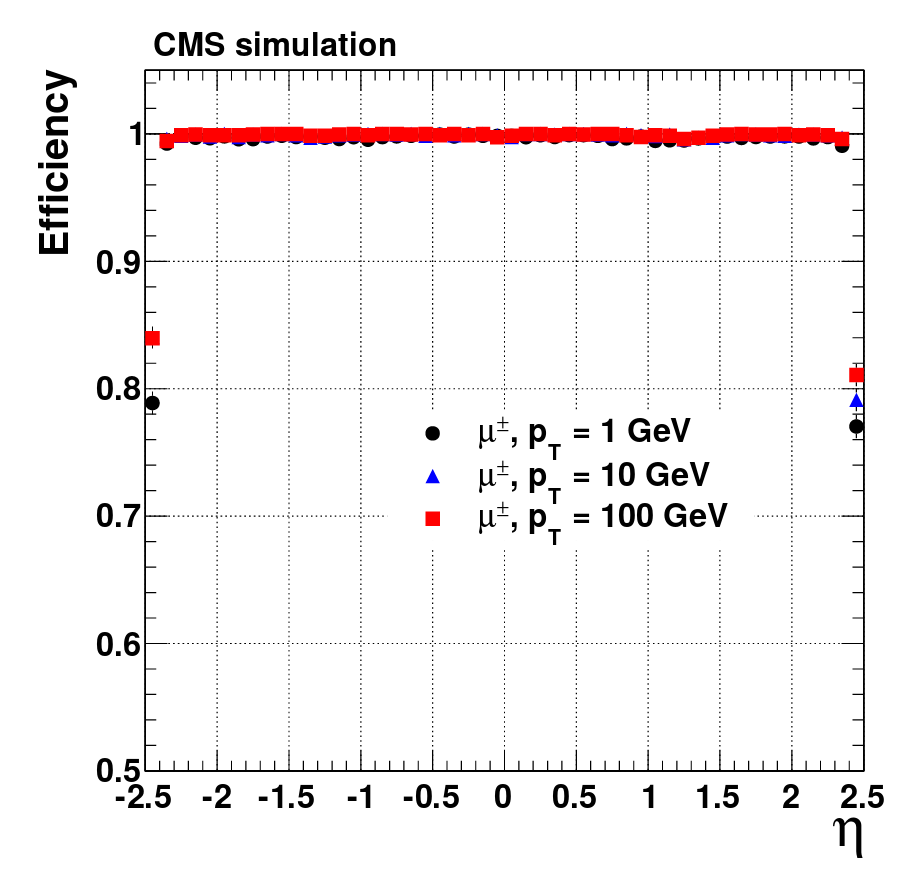
\includegraphics[width=.4\textwidth]{muon_eff_eta}\hspace{1cm}
%  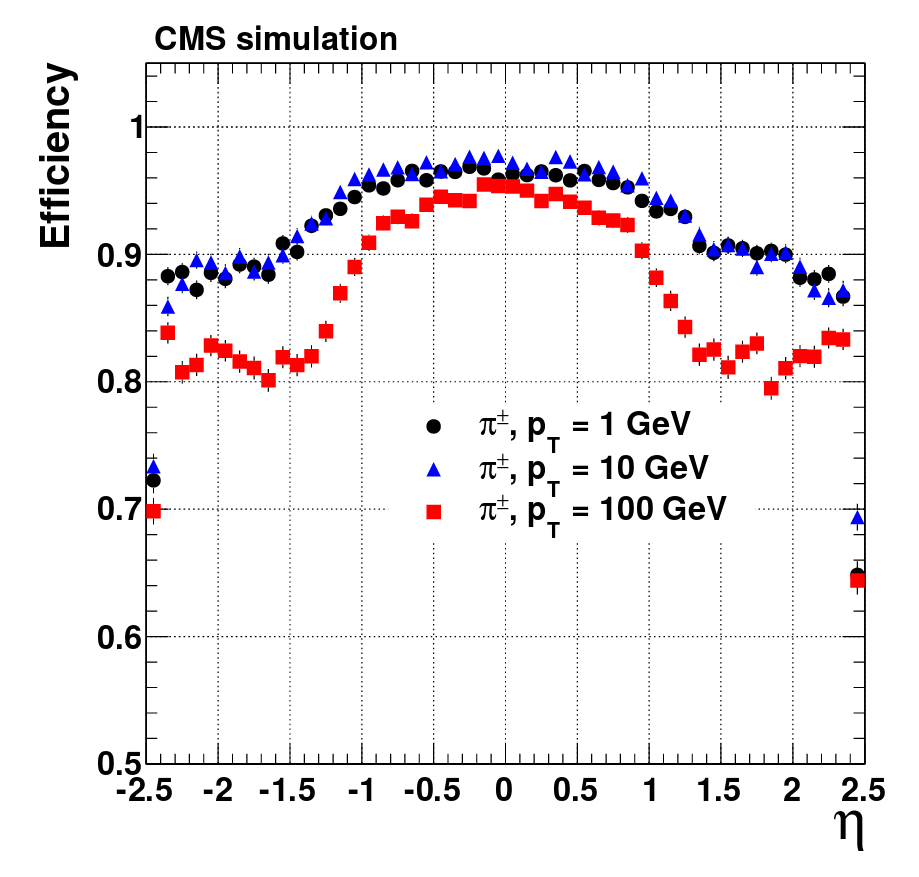
\includegraphics[width=.4\textwidth]{pion_eff_eta} 
%  \caption{The muon efficiency (left) and pion efficiency (right) as a function of pseudorapidity, for multiple transverse momenta.~\cite{Chatrchyan:2014fea}}
%  \label{fig:eff_eta}
% \end{figure}
% 
% Finally, the primary vertex is reconstructed from the tracks. Since the collisions happen between bunches of protons, multiple protons will be colliding at the same time. The extra collisions, next to the potentially interesting collision, are referred to as pile-up interactions. The particles generated in these collisions are all detected simultaneously and form a challenge to disentangle them from the particles coming from the to be studied interaction.
% 
% The reconstruction is done in 2 steps: first the tracks that appear to originate from the same interaction vertex are clustered, then a fitting procedure computes the vertex parameters and assigns a weight to each associated track, reflecting the probability that it corresponds to the considered vertex. Figure~\ref{fig:PV} shows the reconstruction efficiency and the resolution of the primary vertex. The more tracks, the better the vertex is constrained and thus the better the resolution.
% 
% \begin{figure}[ht]
%   \centering
% 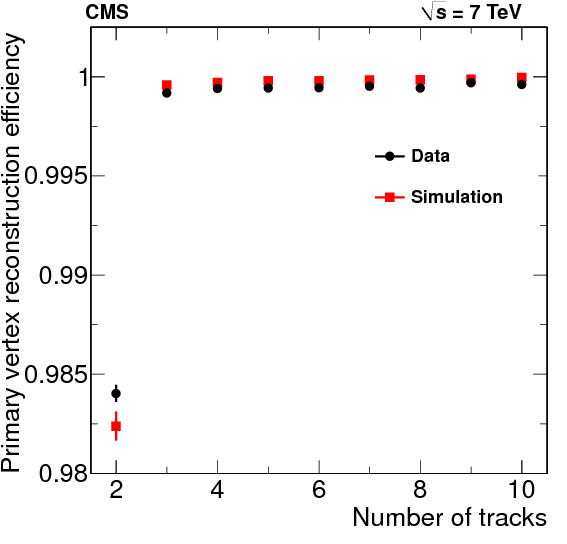
\includegraphics[width=.4\textwidth]{PV_eff}\hspace{1cm}
%  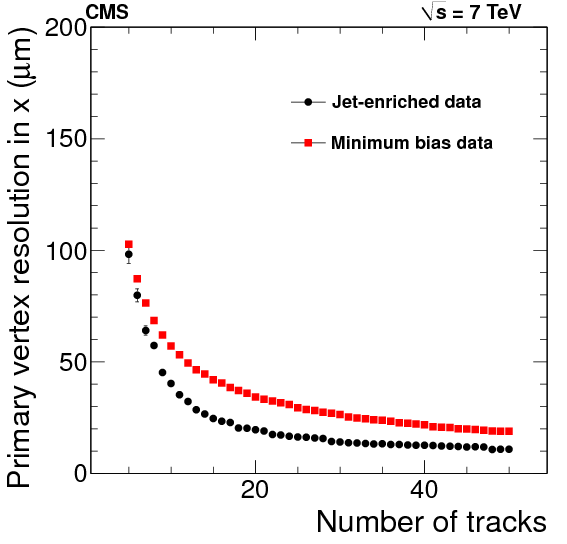
\includegraphics[width=.4\textwidth]{PV_res} 
%  \caption{The primary vertex reconstruction efficiency (left) and resolution (right) as a function of the number of tracks associated to it.~\cite{Chatrchyan:2014fea}}
%  \label{fig:PV}
% \end{figure}

\subsection{The electromagnetic calorimeter}

Surrounding the tracker, the \ac{CMS} \acf{ECAL} is designed to measure the energy of photons and electrons. It is composed of 75~848~lead tungstate (PbWO$_4$) crystals arranged in a cylindrical barrel and 2 endcaps. The barrel crystals measure $22\times22\, \mathrm{mm}^2$ at the front face of crystal, and $26\times26\, \mathrm{mm}^2$ at the rear face, which corresponds to approximately $0.0174\times0.0174$ in $\eta$-$\phi$. The length of the crystal is \SI{230}{mm}, corresponding to $25.8$ radiation lengths. In the endcaps, the crystals have a rear face cross section of $30\times30\, \mathrm{mm}^2$, front face cross section of $28.62\times28.62\, \mathrm{mm}^2$, and a length of \SI{220}{mm}, corresponding to 24.7 radiation lengths. 

The high density material was chosen due to its short radiation length and small Moli\'ere radius, resulting in a small spread of the electromagnetic shower generated by an incoming photon or electron. This allows for a fine granularity, a better shower separation, and a compact calorimeter. Additionally, this scintillating material has a fast response, as about 80\% of the light is emitted during the first \SI{25}{ns}. The scintillation light is collected by photodetectors, digitized, and read out.

The layout of the \ac{ECAL} is shown in Figure~\ref{fig:ecal}, with the barrel (EB) extending up to $|\eta| < 1.470$ and the endcaps (EE) on each side covering the range $1.479 < |\eta| < 3.0$. A preshower detector (ES) is positioned in front of the endcap crystals, covering the pseudorapidity range between $|\eta|=1.653$ and $|\eta| = 2.6$. This detector consists of a layer of lead which initiates an electromagnetic shower from incoming photons or electrons, and a layer of silicon sensors which measures the deposited energy. The main goal of this 20~cm thick detector is to discriminate between photons and neutral pions.

\begin{figure}[ht]
 \centering
 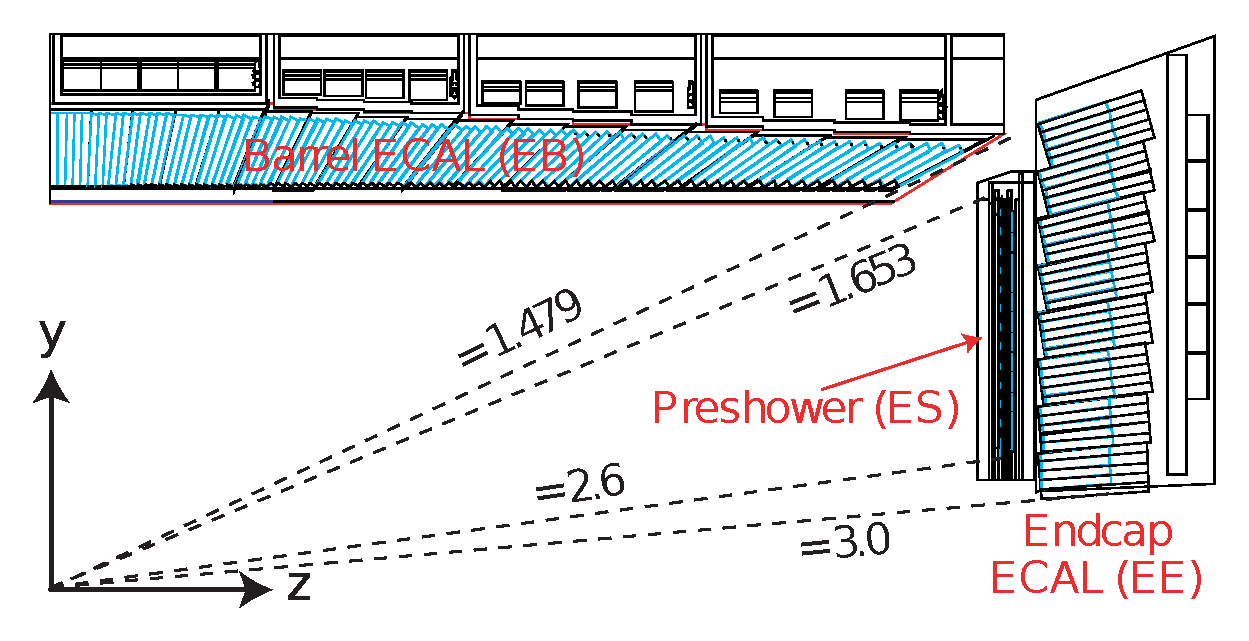
\includegraphics[width = .8\textwidth]{Transverse_section}
\caption{A transverse view parallel to the beamline showing one quarter of the \ac{ECAL}, with its barrel (EB), endcap (EE), and preshower (ES) detectors.}
\label{fig:ecal}
\end{figure}

The energy resolution of calorimeters can be parametrized by the following stochastic ($S$), noise ($N$), and constant ($C$) terms:
\begin{equation}
\label{eq:energy_resolution}
 \left(\frac{\sigma}{E}\right)^2 = \left(\frac{S}{\sqrt{E}}\right)^2 + \left(\frac{N}E{}\right)^2 + C^2
\end{equation}
The stochastic term represents contributions from the shower containment, the number of photoelectrons and the fluctuations in the gain process.  The noise term takes into account all noise components, such as electronics and digitization noise. Finally, the constant term characterizes among others energy leakage from the back of the calorimeter crystals and non-uniformities of the longitudinal light collection. The latter term dominates the energy resolution for high-energy electron and photon showers. Figure~\ref{fig:ecal_res} shows the energy dependence of this resolution for incident electrons as measured in a beam test, as well as the determined stochastic, noise, and constant terms obtained by fitting  equation~\ref{eq:energy_resolution} to the data.

\begin{figure}[ht]
 \centering
 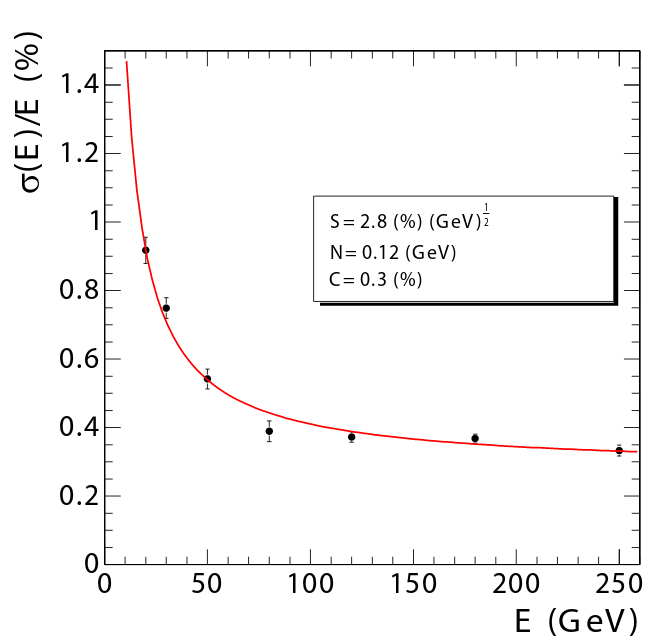
\includegraphics[width = .6\textwidth]{ecal_res}
\caption{The \ac{ECAL} energy resolution as a function of the electron energy, measured from a beam test. The stochastic ($S$), noise ($N$), and constant ($C$) are given as well.}
\label{fig:ecal_res}
\end{figure}

A more recent measurement of the energy resolution was performed using electrons from Z boson decays in collision data. In the central region, up to $|\eta| < 0.8$, it was measured to be better than 2\%. Outside of this region, in the more forward direction, the energy resolution is 2-5\%~\cite{Chatrchyan:2013dga}. The reconstruction of the electrons and photons will be discussed in Section~\ref{sec:electron_reconstruction}.

\subsection{The hadronic calorimeter}

The \acf{HCAL} surrounds the \ac{ECAL} with the aim to measure the energy of charged and neutral hadrons. The missing transverse energy can then be inferred from this measurement together with the measured energy in the \ac{ECAL}, in order to identify neutrinos or exotic particles. The \ac{HCAL} consists of brass absorber plates interleaved with plastic scintillator tiles.

Figure~\ref{fig:hcal} shows a longitudinal quarter view of the different \ac{HCAL} components. A cylindrical barrel (HB) covers the region up to $|\eta| < 1.4$ and is complemented by endcaps (HE) on each side, extending the pseudorapidity range to $|\eta| < 3.0$. In the central region, the stopping power of the \ac{ECAL} and \ac{HCAL} barrel is not sufficient to contain the entire hadron showers. The \ac{HCAL} was therefore extended outside the solenoid with an outer calorimeter (HO), which uses the the magnet coil as absorber and consists of scintillators. Two layers are positioned at $\eta = 0$, where the absorber depth is minimal, and only 1 layer is used for the 2 rings on each side of the central ring. Finally, a forward calorimeter (HF) is positioned at 11.2~m from the \ac{IP} covering $3.0 < |\eta| < 5.2$. Unlike the other \ac{HCAL} components, this detector consists of iron and quartz fibers. Cherenkov-based, radiation-hard technology, since it is exposed to very large particle fluxes. 
% Additionally, the forward detector is used as luminosity monitor.

\begin{figure}[ht]
  \centering
 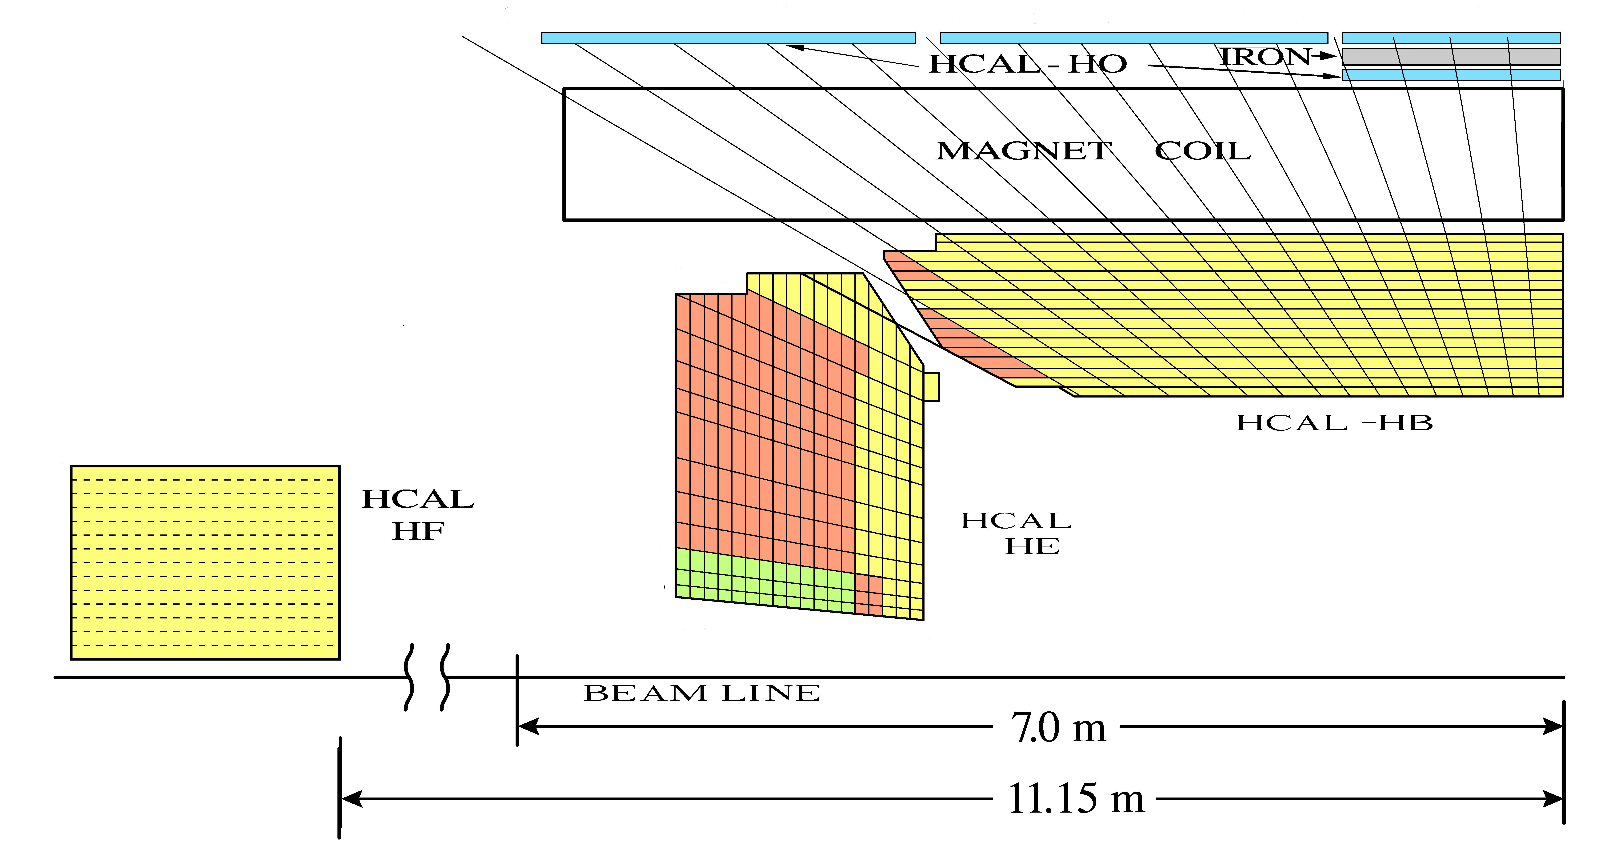
\includegraphics[width=.8\textwidth]{hcal}
 \caption{A quarter view of the \protect\acf{HCAL}, parallel to the beamline. The barrel (HB), endcap (HE), outer (HO), and forward (HF) detectors are indicated.}
 \label{fig:hcal}
\end{figure}

The optical signals from the scintillators in the HB and HE are converted to electrical signals by multichannel hybrid photodiodes, while silicon photomultipliers (SiPMs) are used in the HO. In the HF, the Cherenkov light emitted in the quartz fibers is detected by standard photomultiplier tubes (PMTs), since the magnetic field is much smaller in this region.

The expected transverse energy resolution for jets is shown in Figure~\ref{fig:JER} for various pseudorapidity regions: barrel jets ($|\eta| < 1.4$), endcap jets ($1.4 < |\eta| < 3.0$), and very forward jets ($3.0 < |\eta| < 5.0$). Details about the reconstruction of jets from calorimeter and tracking information will be given in Section~\ref{sec:jet_reconstruction}.

\begin{figure}[ht]
  \centering
 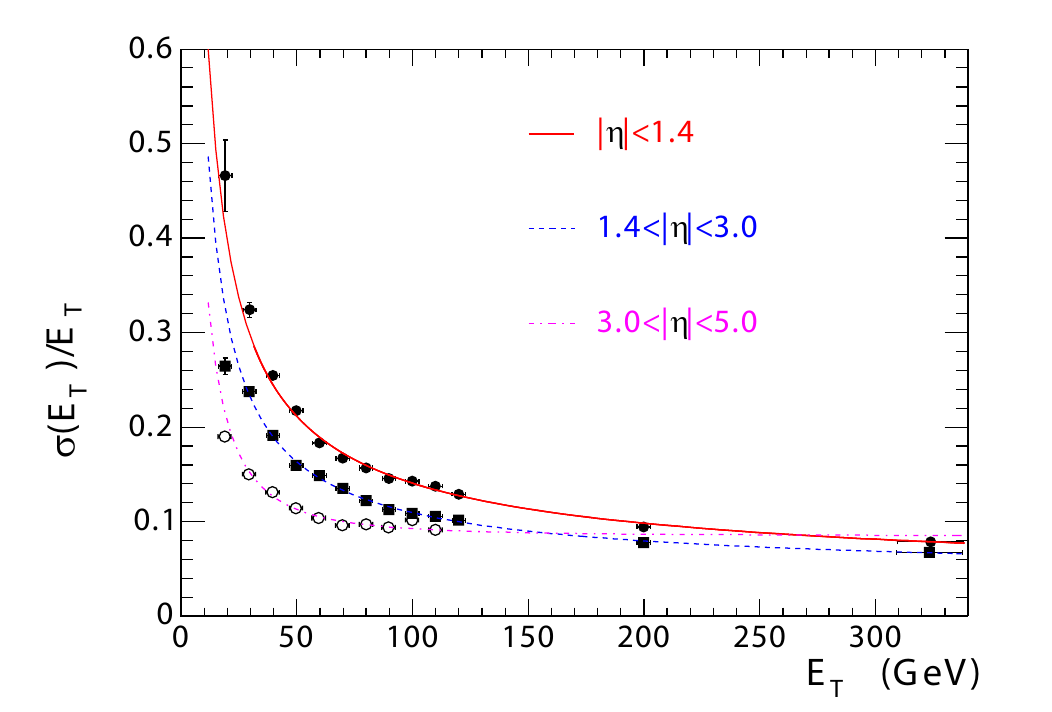
\includegraphics[width=.6\textwidth]{JER}
 \caption{The jet transverse energy resolution as a function of the jet transverse energy, for barrel jets ($|\eta| < 1.4$), endcap jets ($1.4 < |\eta| < 3.0$), and very forward jets ($3.0 < |\eta| < 5.0$).}
 \label{fig:JER}
\end{figure}

\subsection{The muon system}

The outermost detector, located entirely on the outside of the solenoid, is a dedicated muon detection system. The purpose of this subsystem is muon identification, momentum measurement, and triggering. As illustrated in Figure~\ref{fig:muons}, the layers of muon chambers are embedded in the iron yoke constraining the magnetic field lines. The strong magnetic field completely saturates the return yoke with a field of about \SI{2}{T}, in opposite direction with respect to the field inside the magnet.

\begin{figure}[ht]
  \centering
 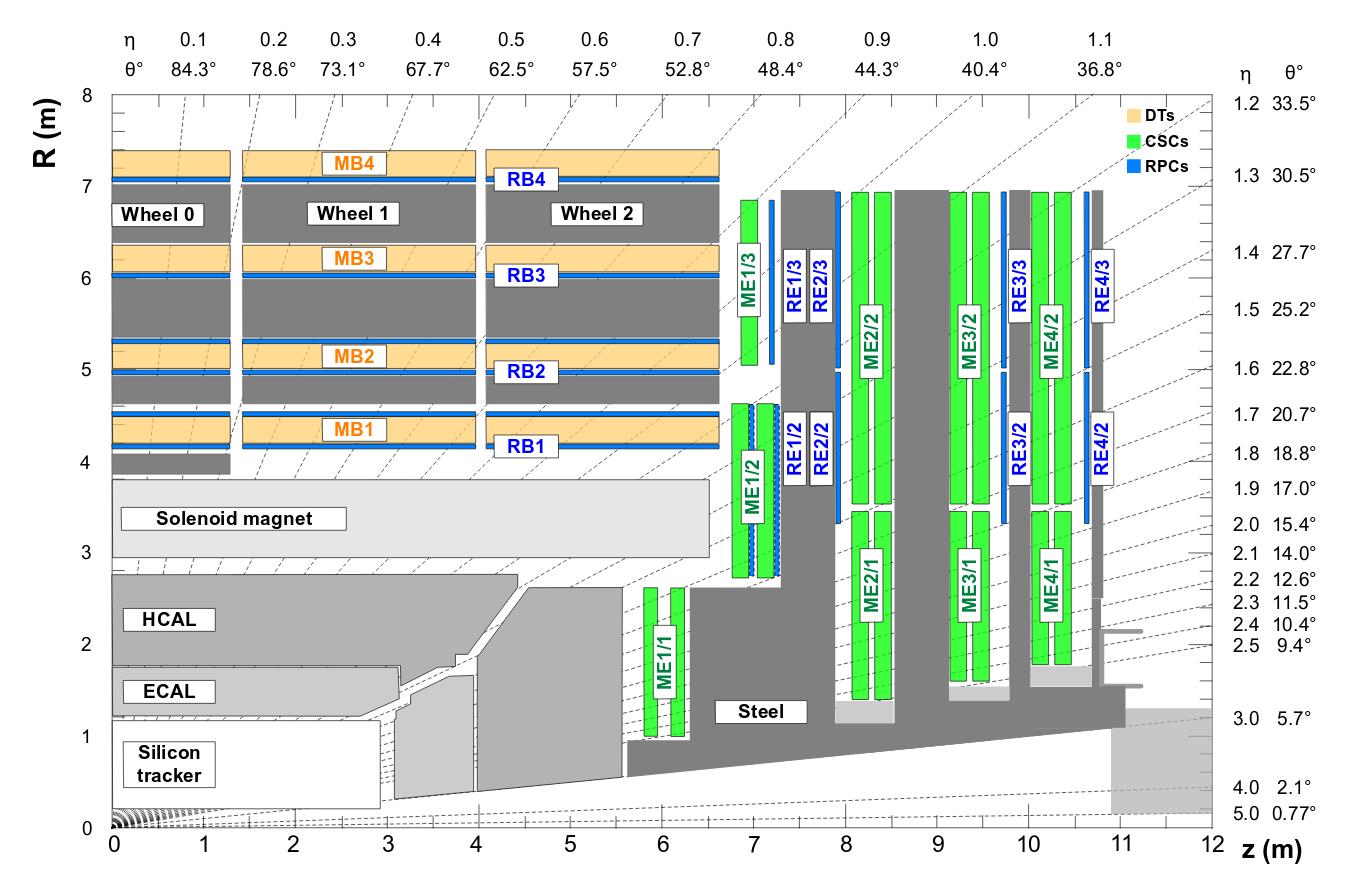
\includegraphics[width=.9\textwidth]{muon_system_new}
 \caption{A transverse view of one quarter of \ac{CMS} showing the position of the 3 types of muon detectors. The \protect\acf{DT} are located in the barrel, the \protect\acf{CSC} in the endcaps, and the \protect\acf{RPC} in both regions up to $|\eta| < 1.8$.}
 \label{fig:muons}
\end{figure}

Three different types of gaseous detectors are used. In the barrel, 4 layers of \ac{DT} are installed, covering the pseudorapidity range up to $|\eta| < 1.2$. Due the higher flux and the larger and non-uniform magnetic field at larger pseudorapidities, \ac{CSC} are used in the endcap region ($0.9 < |\eta| < 2.4$). The \acp{DT} are designed for the low muon rates that are expected in the barrel and thus have a slower response time than the \acp{CSC}. \acp{RPC} complement the \ac{DT} and \ac{CSC} systems in the pseudorapidity region up to $|\eta| < 1.8$. They provide a fast response, with a good time resolution but a worse spatial resolution than the \acp{DT} or \acp{CSC}. The \acp{RPC} are therefore very well suited to trigger on muons.

The offline reconstruction efficiency of simulated events containing one muon is typically between 95\% and 99\%, except for the regions between 2 \ac{DT} wheels ($|\eta| = 0.25$ and $|\eta| = 0.8$) and the transition region between the \acp{DT} and \acp{CSC} ($|\eta| = 1.2$), where the efficiency drops to 92\%. The reconstruction of muons using the information from the tracker and the muon detectors will be detailed in Section~\ref{sec:muon_reconstruction}. For low pseudorapidities and small momenta, the offline momentum resolution of the standalone muon system is about 9\%. At momenta around \SI{1}{TeV}, the resolution varies from 15\% to 40\%, depending on the pseudorapidity. As demonstrated in Figure~\ref{fig:muon_res}, performing a global momentum fit using the tracker as well improves the resolution by an order of magnitude at low muon momenta. At high momenta the resolution of the full system is about 5\%.

\begin{figure}[ht]
  \centering
 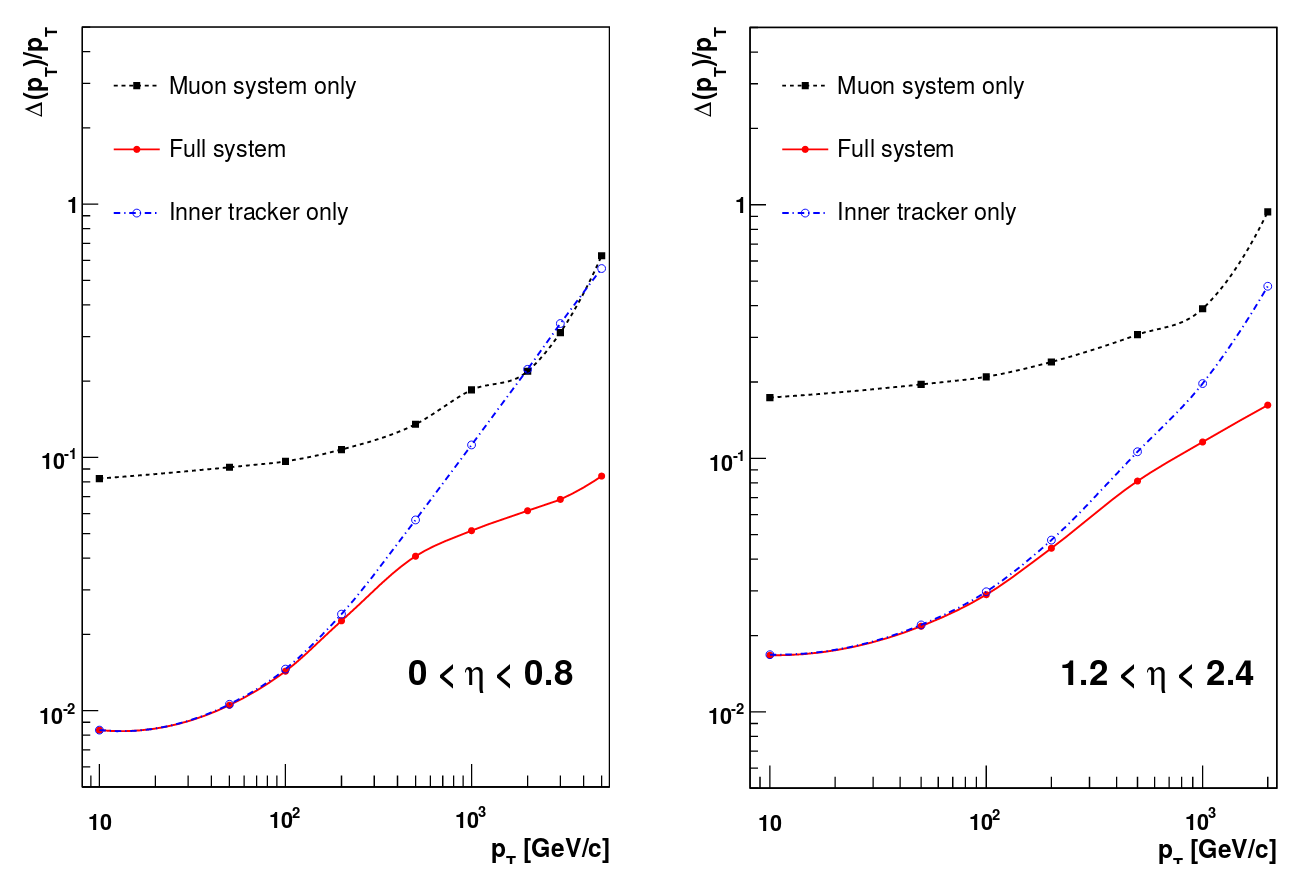
\includegraphics[width=.9\textwidth]{muon_res}
 \caption{The muon transverse momentum resolution as a function of transverse momentum for low (left) and (high) pseudorapidities. The resolution is shown for the muon system and the tracker separately, and for the full system.~\cite{Chatrchyan:2008aa}}
 \label{fig:muon_res}
\end{figure}

\subsection{Trigger and data acquisition}

Collisions are provided by the \ac{LHC} at high interaction rates, with an interval of \SI{25}{ns} between bunch crossings. This corresponds to a frequency of \SI{40}{MHz}. Additionally, multiple collisions occur at the same time, depending on the luminosity. Since it is impossible to store and process the large amount of data produced in the collisions at this high rate, a severe rate reduction is needed. This rate reduction is performed by the trigger system, which decides whether to store or reject an event. Since this decision process is constrained in time, the computing time is optimized by rejecting uninteresting events as quickly as possible. The rate is reduced to \SI{1}{kHz} in two steps by the \ac{L1} Trigger and the \ac{HLT}.

The \ac{L1} Trigger decision is based on information from the calorimeters and muon systems, following the structure illustrated in Figure~\ref{fig:L1}. At the lowest level, the Local Triggers are based on energy deposits in calorimeter towers and track segments or hit patterns in the muon system. Regional triggers, indicated as Calo Trigger Layer 1 and Muon Track-Finder Layer in the figure, then combine this information and use pattern logic to determine trigger objects such as jet or muon candidates in separated spatial regions. The candidates are ranked based on their energy or momentum and quality, reflecting the level of confidence assigned to the \ac{L1} parameter measurements. Finally, the Calo Trigger Layer 2 and the Global Muon Trigger~(GMT) determine the highest-rank calorimeter and muon objects across the whole detector and transfer them to the Global Trigger, which makes the final decision to accept or reject an event. Following this procedure, the \ac{L1} Trigger thresholds are tuned to reduce the event rate to 100~kHz. The \ac{L1} Trigger is composed of custom electronics located partially on the detectors, and partially in the underground service cavern. The \ac{L1} decision needs to be made and distributed to the detector front-end electronics within 3.8~$\mu$s~\cite{Tapper:2013yva}.

\begin{figure}[ht]
  \centering
 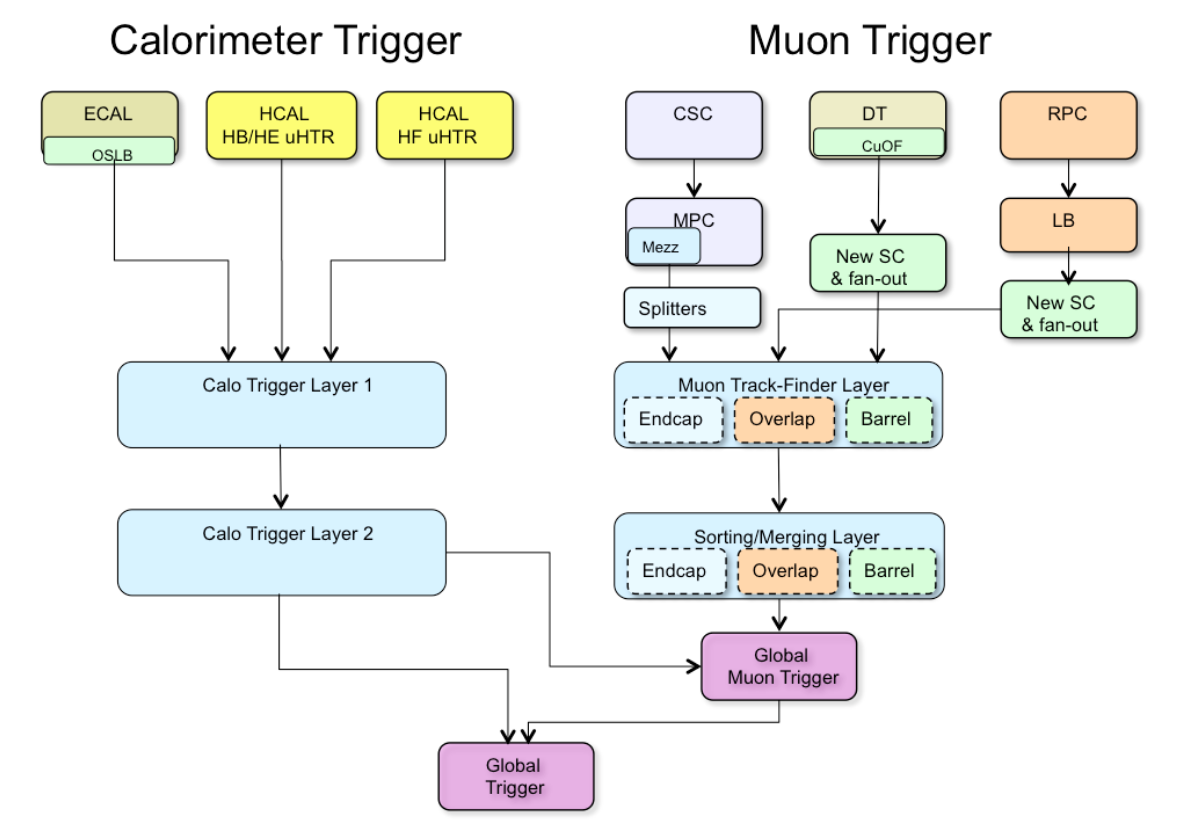
\includegraphics[width=.9\textwidth]{trigger}
 \caption{Schematic overview of the \ac{L1} Trigger.~\cite{Tapper:2013yva}}
 \label{fig:L1}
\end{figure}
 % figure from: http://cds.cern.ch/record/2238553/files/CR2016_412.pdf
 
The readout of the data proceeds as illustrated in Figure~\ref{fig:DAQ}. When an event is accepted by the \ac{L1} Trigger, the data from about $740$ \acp{FED} is read out by the \acp{RU}. For so-called {\it legacy} systems, i.e. systems which are using VME-based hardware from the initial installation, the \acp{FED} are read out by custom Front-End-Readout-Link (FRL) cards, while for systems that changed their readout architecture from the VME standard to the newer $\rm \mu{}$TCA standard during or after LS1 they are read out via the newer Front-End-Readout-Optical-Link (FEROL) cards. The event fragments are then sent over the event-builder switch to the \acp{BU}, which assemble the events. Next, the events are distributed to the \acp{FU} by a large switch network.

\begin{figure}[ht]
  \centering
 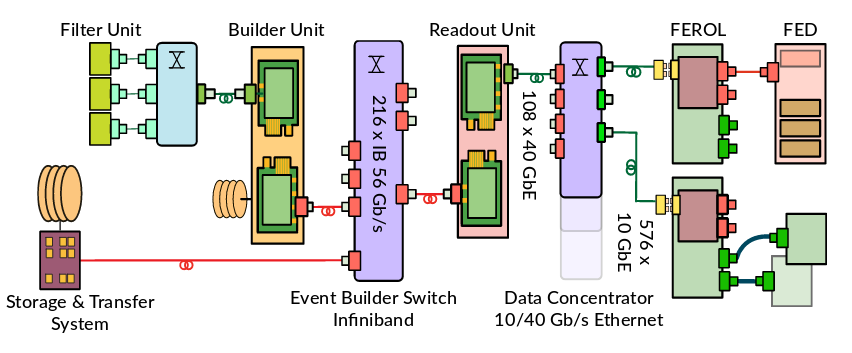
\includegraphics[width=.9\textwidth]{DAQ}
 \caption{Schematic of the \protect\acf{DAQ} system.~\cite{Andre:2252634}}
 \label{fig:DAQ}
\end{figure}

The \ac{HLT} software system is implemented in this filter farm, which uses more than 15000 CPU cores for the final event selection. In this second step, the \ac{HLT} reduces the event rate further to \SI{1}{kHz}. The complete read-out data, including information from the pixel and strip tracker, are available for this step. New objects can therefore be reconstructed such as e.g. tau leptons and b-jets, as is done in the offline software, but speed-optimized.%http://ieeexplore.ieee.org/stamp/stamp.jsp?arnumber=7111380

\subsection{CMS performance in Run 2}

The number of collisions recorded at the experiments will differ from the amount delivered by the \ac{LHC}. Data loss can be caused by e.g. problems with a particular subdetector, the trigger rate, the data acquisition, or the infrastructure. During Run 2, CMS achieved a data taking efficiency of 89\% and 92\% in 2015 and 2016, respectively. The comparison between the delivered and recorded cumulative integrated luminosity in 2016 is shown in Figure~\ref{fig:CMSlumi}. Subsequently, the recorded data is certified by the offline \ac{DQM}, to ensure that the data are suited for physics analysis. 

\begin{figure}[ht]
  \centering
 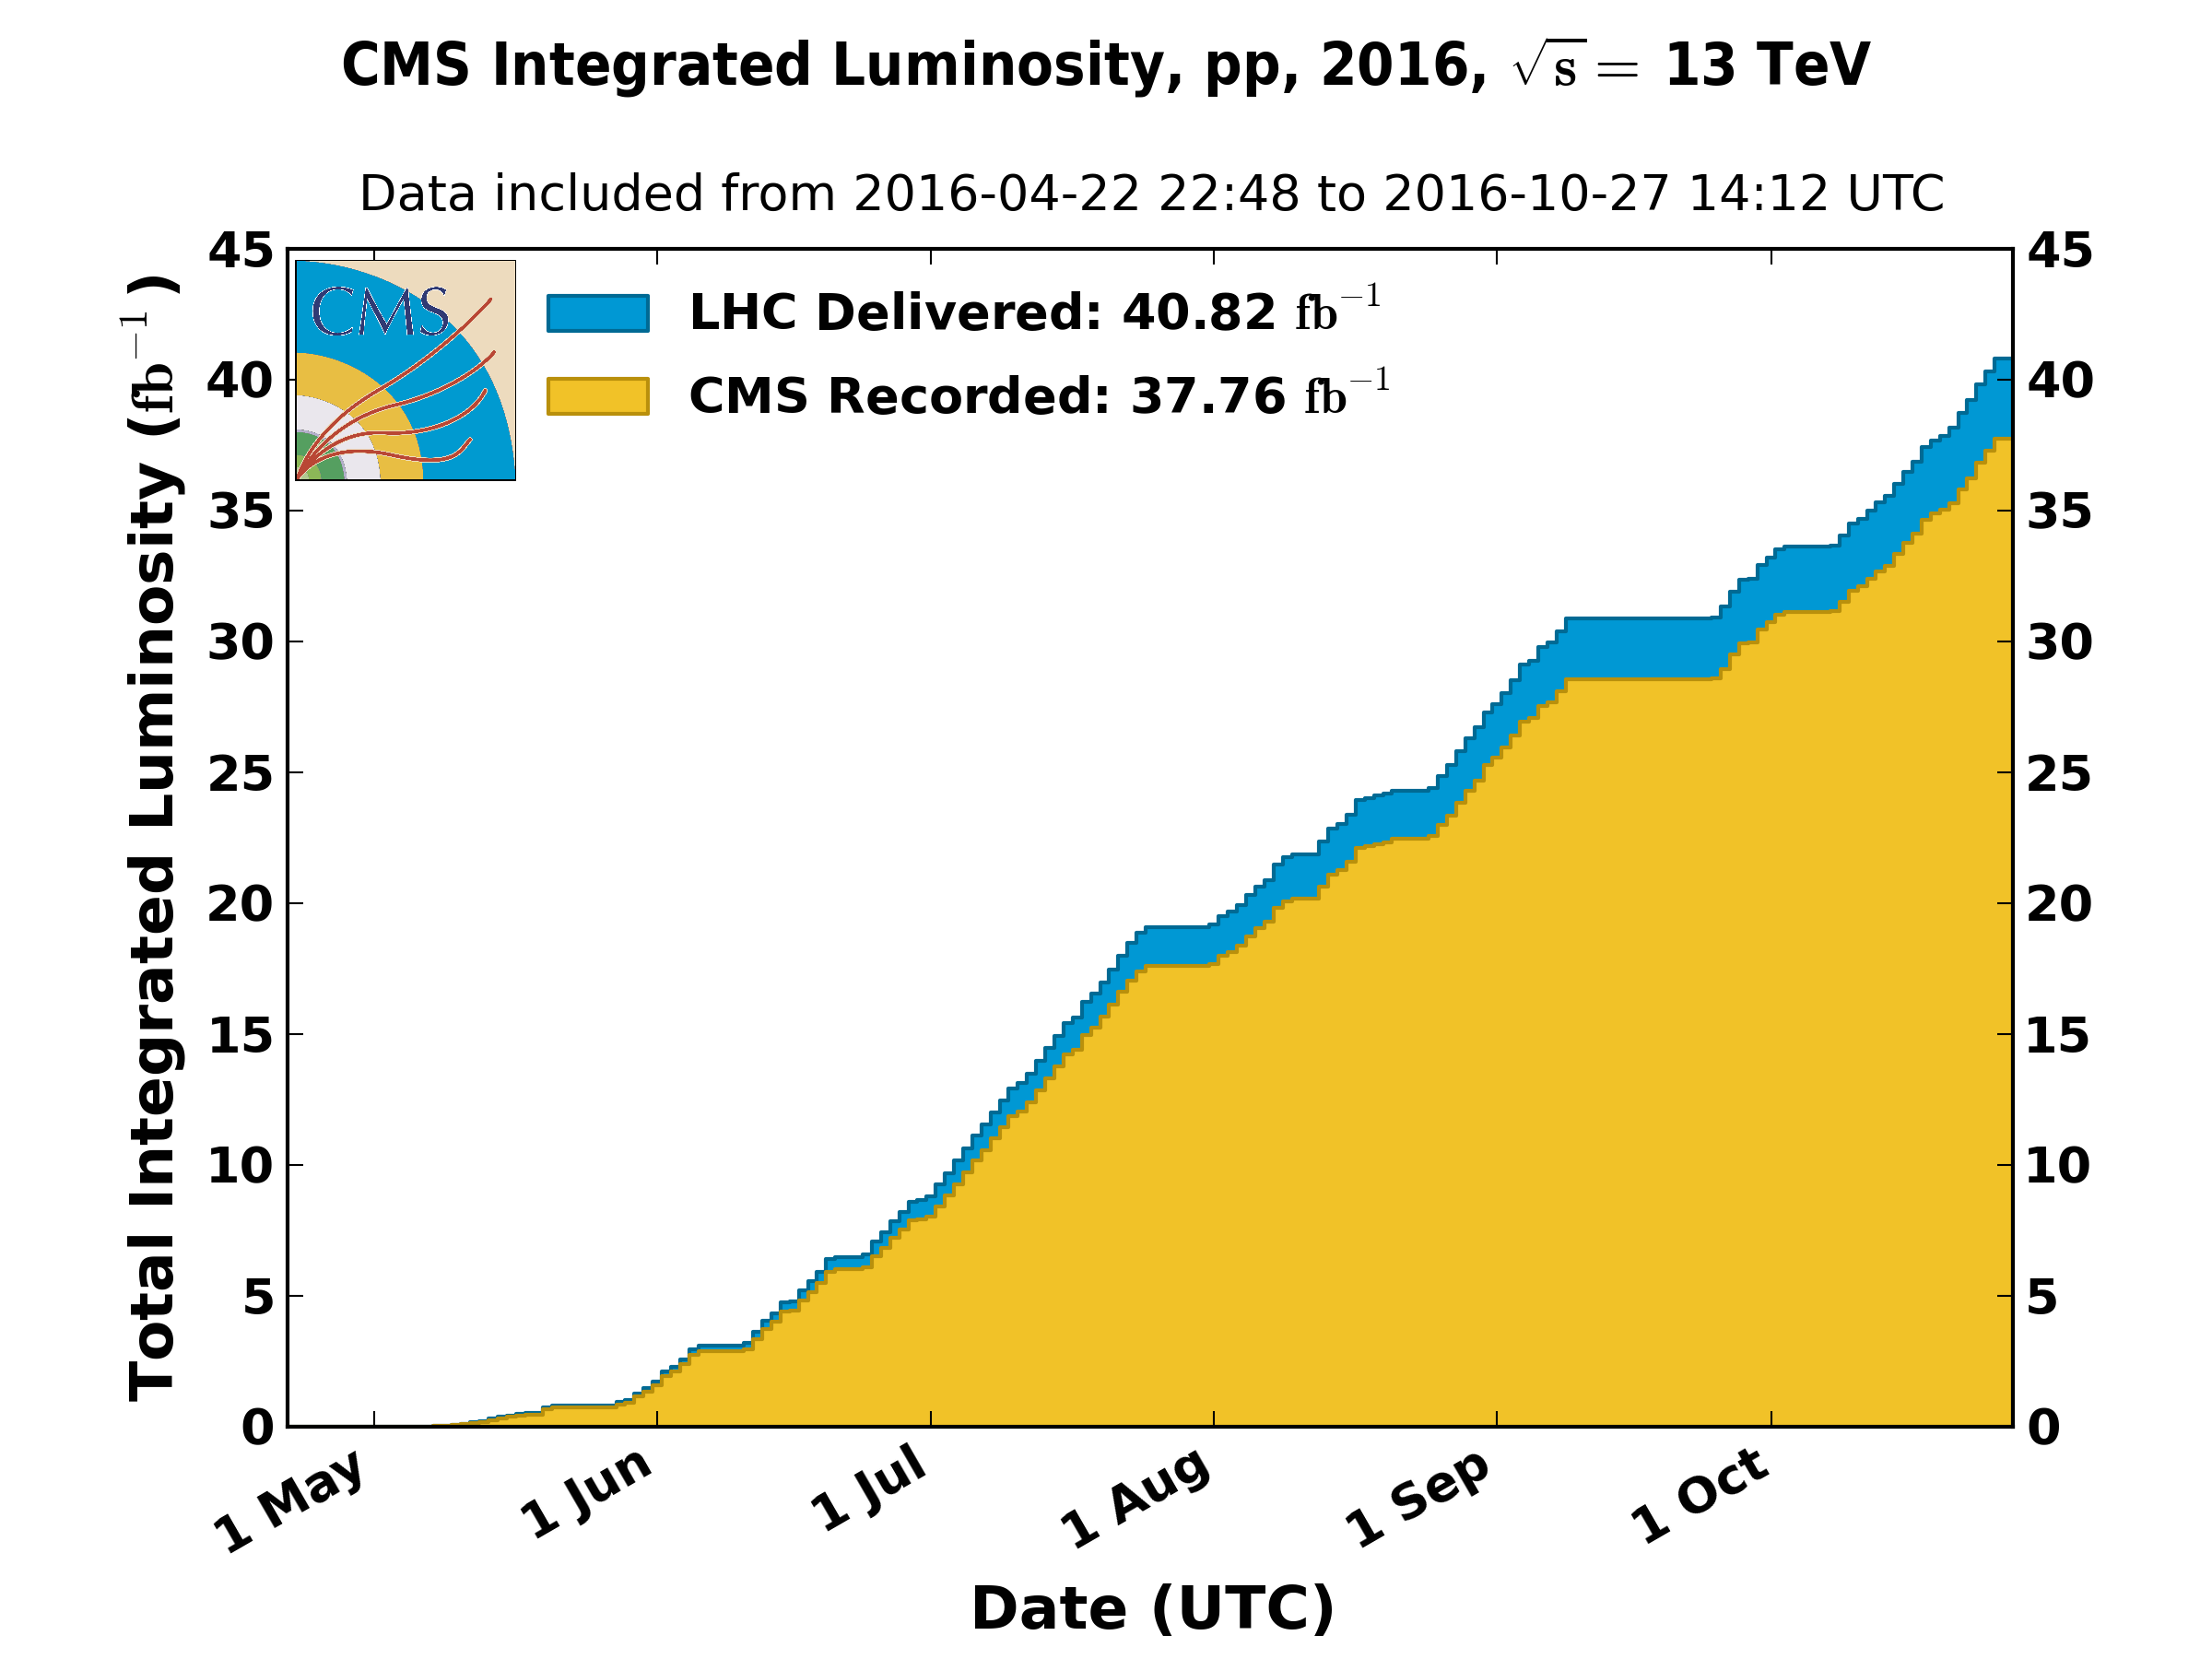
\includegraphics[width=.75\textwidth]{CMS_recorded_lumi}
 \caption{The cumulative distribution of the instantaneous luminosity delivered by the \ac{LHC} (blue) and recorded by \ac{CMS} (yellow) in 2016.}
 \label{fig:CMSlumi}
\end{figure}

\subsubsection{Pre-amplifier saturation in the APV25 chip}

During Run 2, the instantaneous luminosity delivered by the \ac{LHC} increased continuously, and even exceeded the design luminosity of $10^{34}$ cm$^{-2}$s$^{-1}$ in 2016. As the luminosity increased, a dynamic inefficiency appeared in the strip tracker, which was most noticeable in the first layer of the \ac{TOB}. The symptoms were a change in the signal-to-noise ratio and loss of hits. As can be seen from Figure~\ref{fig:SOverN}, the most probable value (MPV) of the signal-to-noise ratio is shifted towards lower values and the low tail increased as well. The loss of hits is clearly visible in Figure~\ref{fig:nhits}, showing the change in number of hits per track for increasing instantaneous luminosities. The run periods indicated in the plot refer to a subset of the data taken over the course of the year. Run period boundaries are typically defined by changes in the \ac{LHC} running conditions, changes to the detector configuration or calibration, or other parameters. The number of hits decreases for later run periods such as D and F, as the instantaneous luminosity increases. This loss of hits results in less and shorter tracks.
  
\begin{figure}[ht]
  \centering
 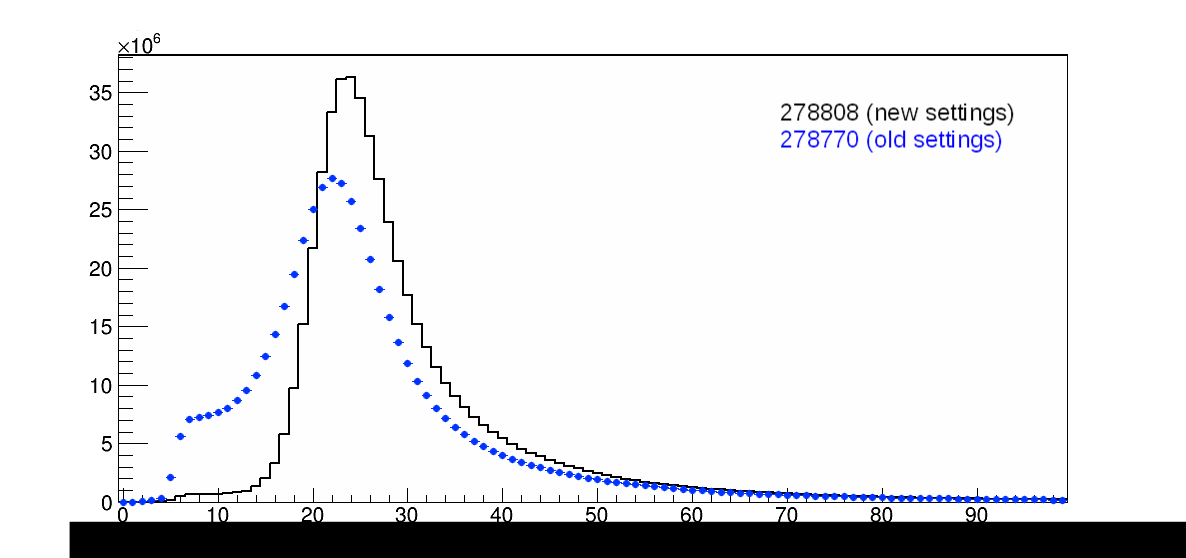
\includegraphics[width=.9\textwidth]{APVsaturation_SOverN}
 \caption{The signal-to-noise ratio for clusters on reconstructed tracks in the first layer of the \ac{TOB} for a run before (blue) and after (black) the change of pre-amplifier drain speed.}
 \label{fig:SOverN}
\end{figure}
  
\begin{figure}[ht]
  \centering
 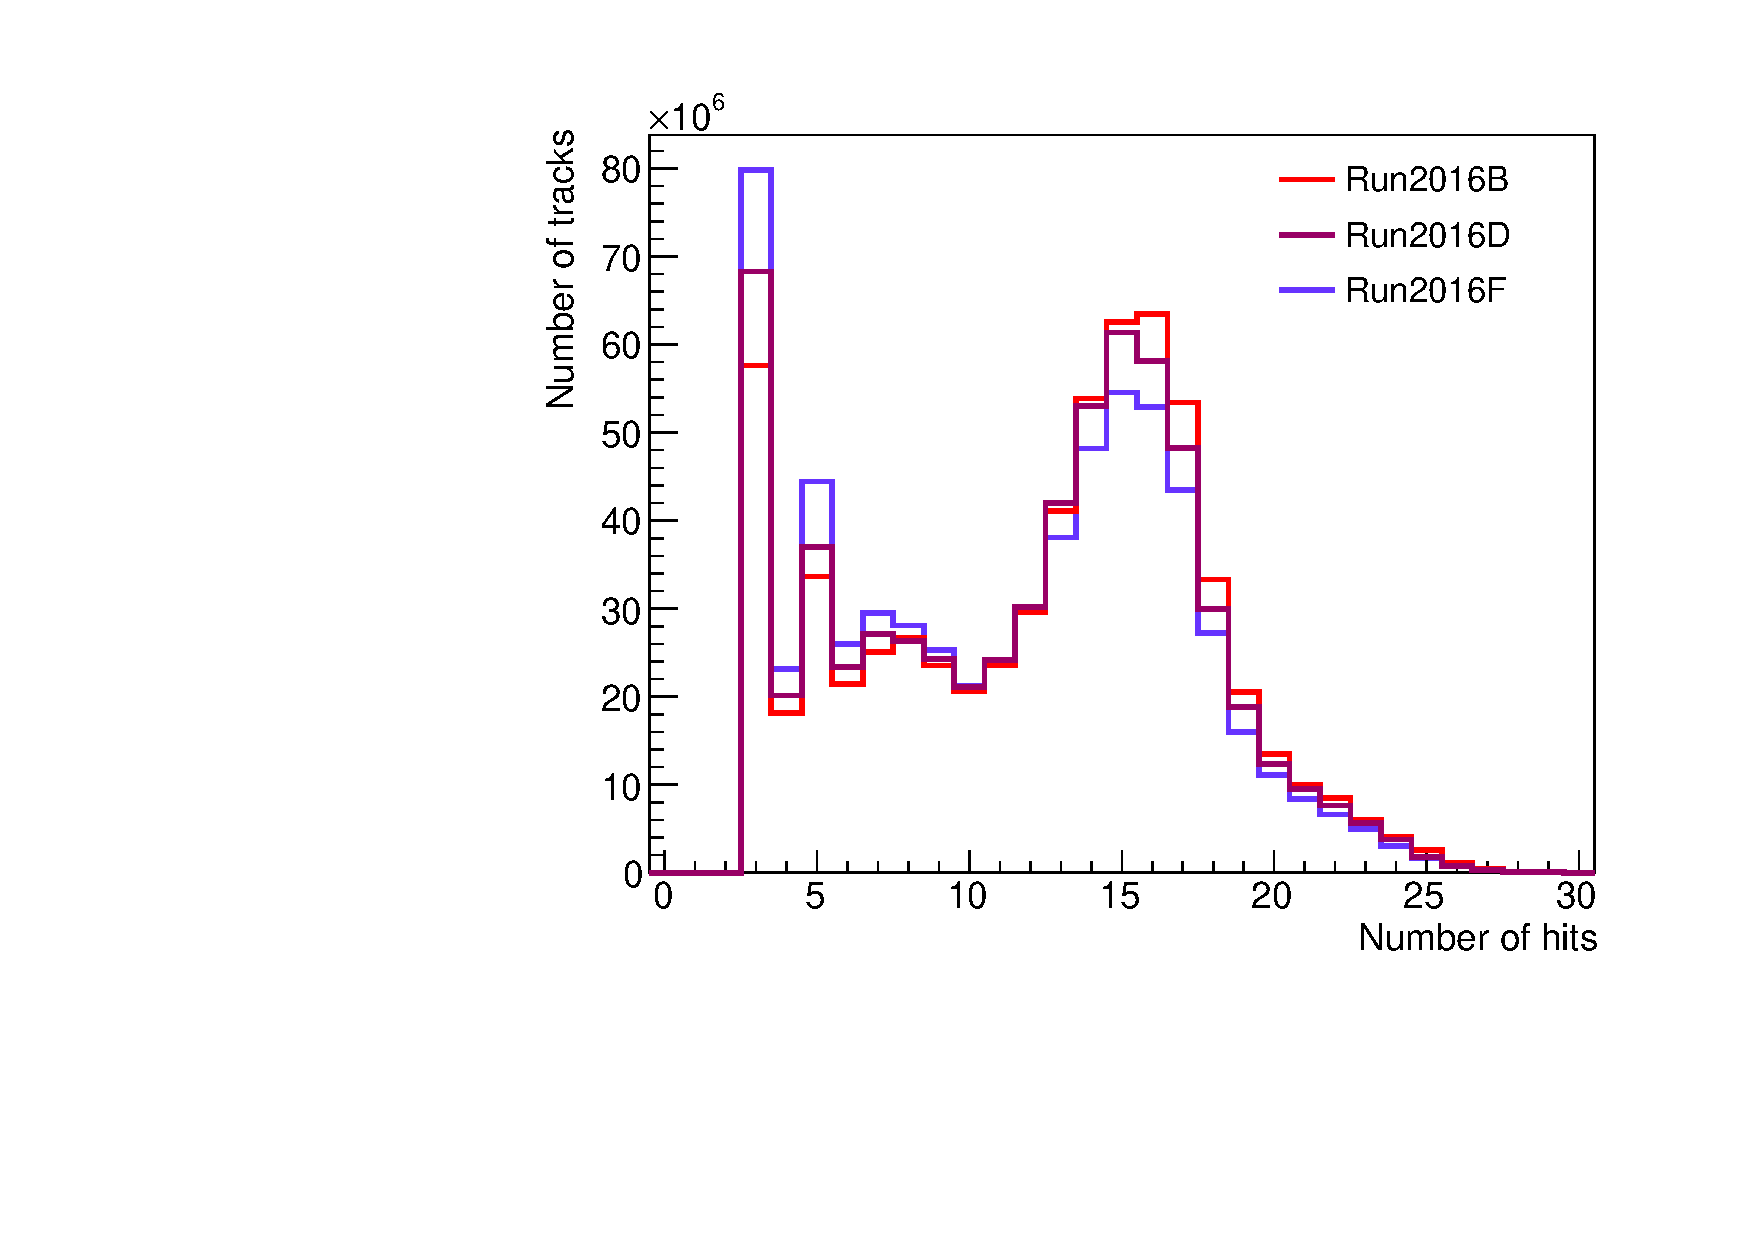
\includegraphics[width=.6\textwidth]{nhits_perRunPeriod}
%  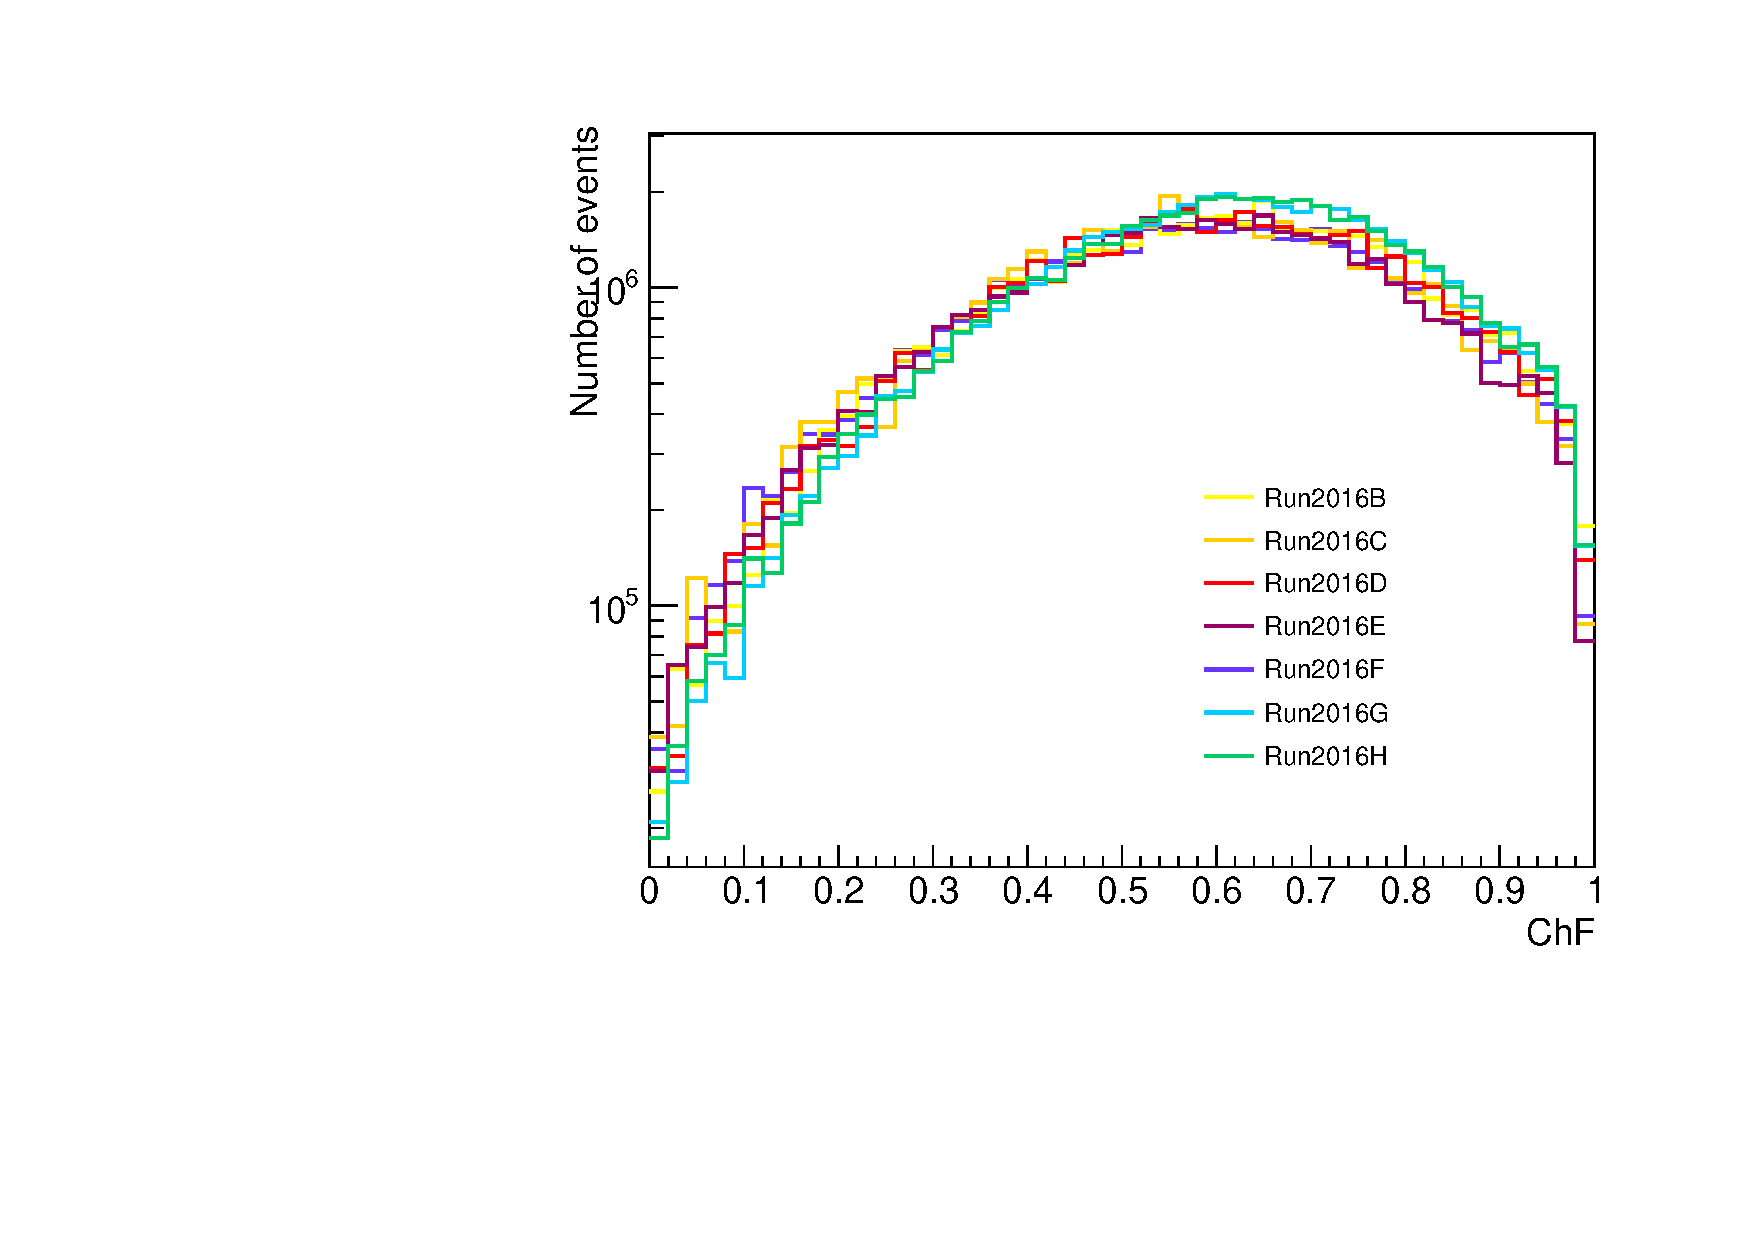
\includegraphics[width=.47\textwidth]{ChF_perRunPeriod}
 \caption{The number of hits per track for run periods B, D, and F, showing the effect of the increasing instantaneous luminosity.}
 \label{fig:nhits}
\end{figure}

The origin of this inefficiency was eventually tracked down to saturation effects in the pre-amplifier of the APV25 chip. The pre-amplifier decay time changes significantly with temperature. As the operating temperature of the strip tracker was lowered from $+4$\degree C to $-15$\degree C coolant temperature during LS1, the decay time was no longer sufficient to cope with the high luminosities. The dynamic inefficiency was cured in August 2016 by changing the pre-amplifier drain speed. This lead among others to the recovery of the muon efficiency, which showed a large drop for the highest luminosities before the change and an essentially flat behavior afterwards, as demonstrated in Figure~\ref{fig:muoneff}.
  
\begin{figure}[ht]
  \centering
 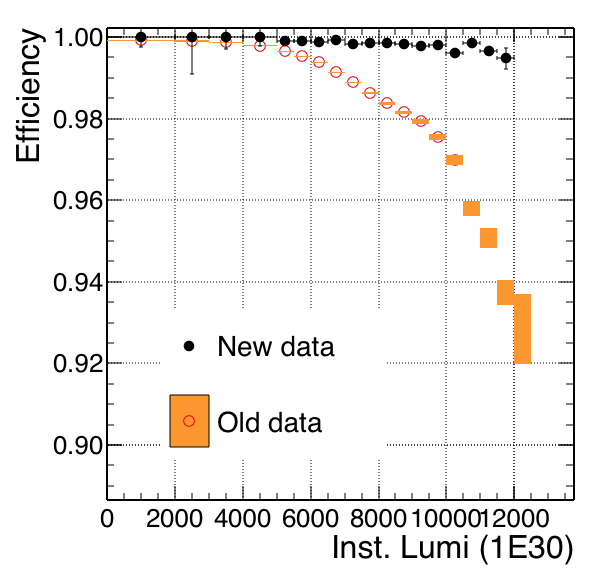
\includegraphics[width=.6\textwidth]{APVsaturation_muoneff}
 \caption{The muon efficiency as a function of the instantaneous luminosity for before (orange) and after (black) the change of pre-amplifier drain speed which cured the dynamic inefficiency.}
 \label{fig:muoneff}
\end{figure}

\clearpage

\clearpage{\pagestyle{empty}\cleardoublepage}

\graphicspath{{chapt_dutch/}{intro/}{detector/}{reconstruction/}}

% Header
\renewcommand\evenpagerightmark{{\scshape\small Chapter 4}}
\renewcommand\oddpageleftmark{{\scshape\small Event Simulation and Reconstruction}}

\hyphenation{}

\chapter{Event Simulation and Reconstruction}
\label{ch:reconstruction}

In order to use the recorded data, the obtained signals coming from various parts of the detector must be reconstructed to be able to identify the particles in the event. Additionally, to compare the experimental results with theory, events are generated and the resulting signals in the detector are simulated, as detailed in Sections~\ref{sec:generation} and \ref{sec:sim}, respectively. The event reconstruction is detailed in Section~\ref{sec:reconstruction}. Finally, some details about the simulation of \acp{SIMP} are given in Section~\ref{sec:SIMPs}.

\section{Event generation}
\label{sec:generation}

% matching?
% meer detail? Fabio, MCnet school

The event structure at the \ac{LHC} is complicated by the composite nature of the colliding protons, as demonstrated in Figure~\ref{fig:event}. This sketch shows the hard interaction in red, with a tree-like structure surrounding it, representing the ensuing shower. In this hard scattering, the quark or gluon constituents of the protons, called partons, will interact according to a so-called \ac{PDF}, which is determined by the parton's momentum fraction and the momentum transfer. Due to their colour charge, the partons involved in the hard interaction will induce parton showers consisting of a cascade of radiation from \acs{QCD} processes. This is shown in blue for the incoming partons and in red for the outgoing partons. The produced partons will also hadronize due to colour confinement, as illustrated in green, with hadron decays in dark green and radiated photons in yellow. Finally, the purple interaction represents a second interaction between the proton remnants. Next to these multiple parton interactions, additional activity in the event can also come from pileup. All these aspects must be taken into account when generating events, as detailed below.

\begin{figure}[ht]
  \centering
 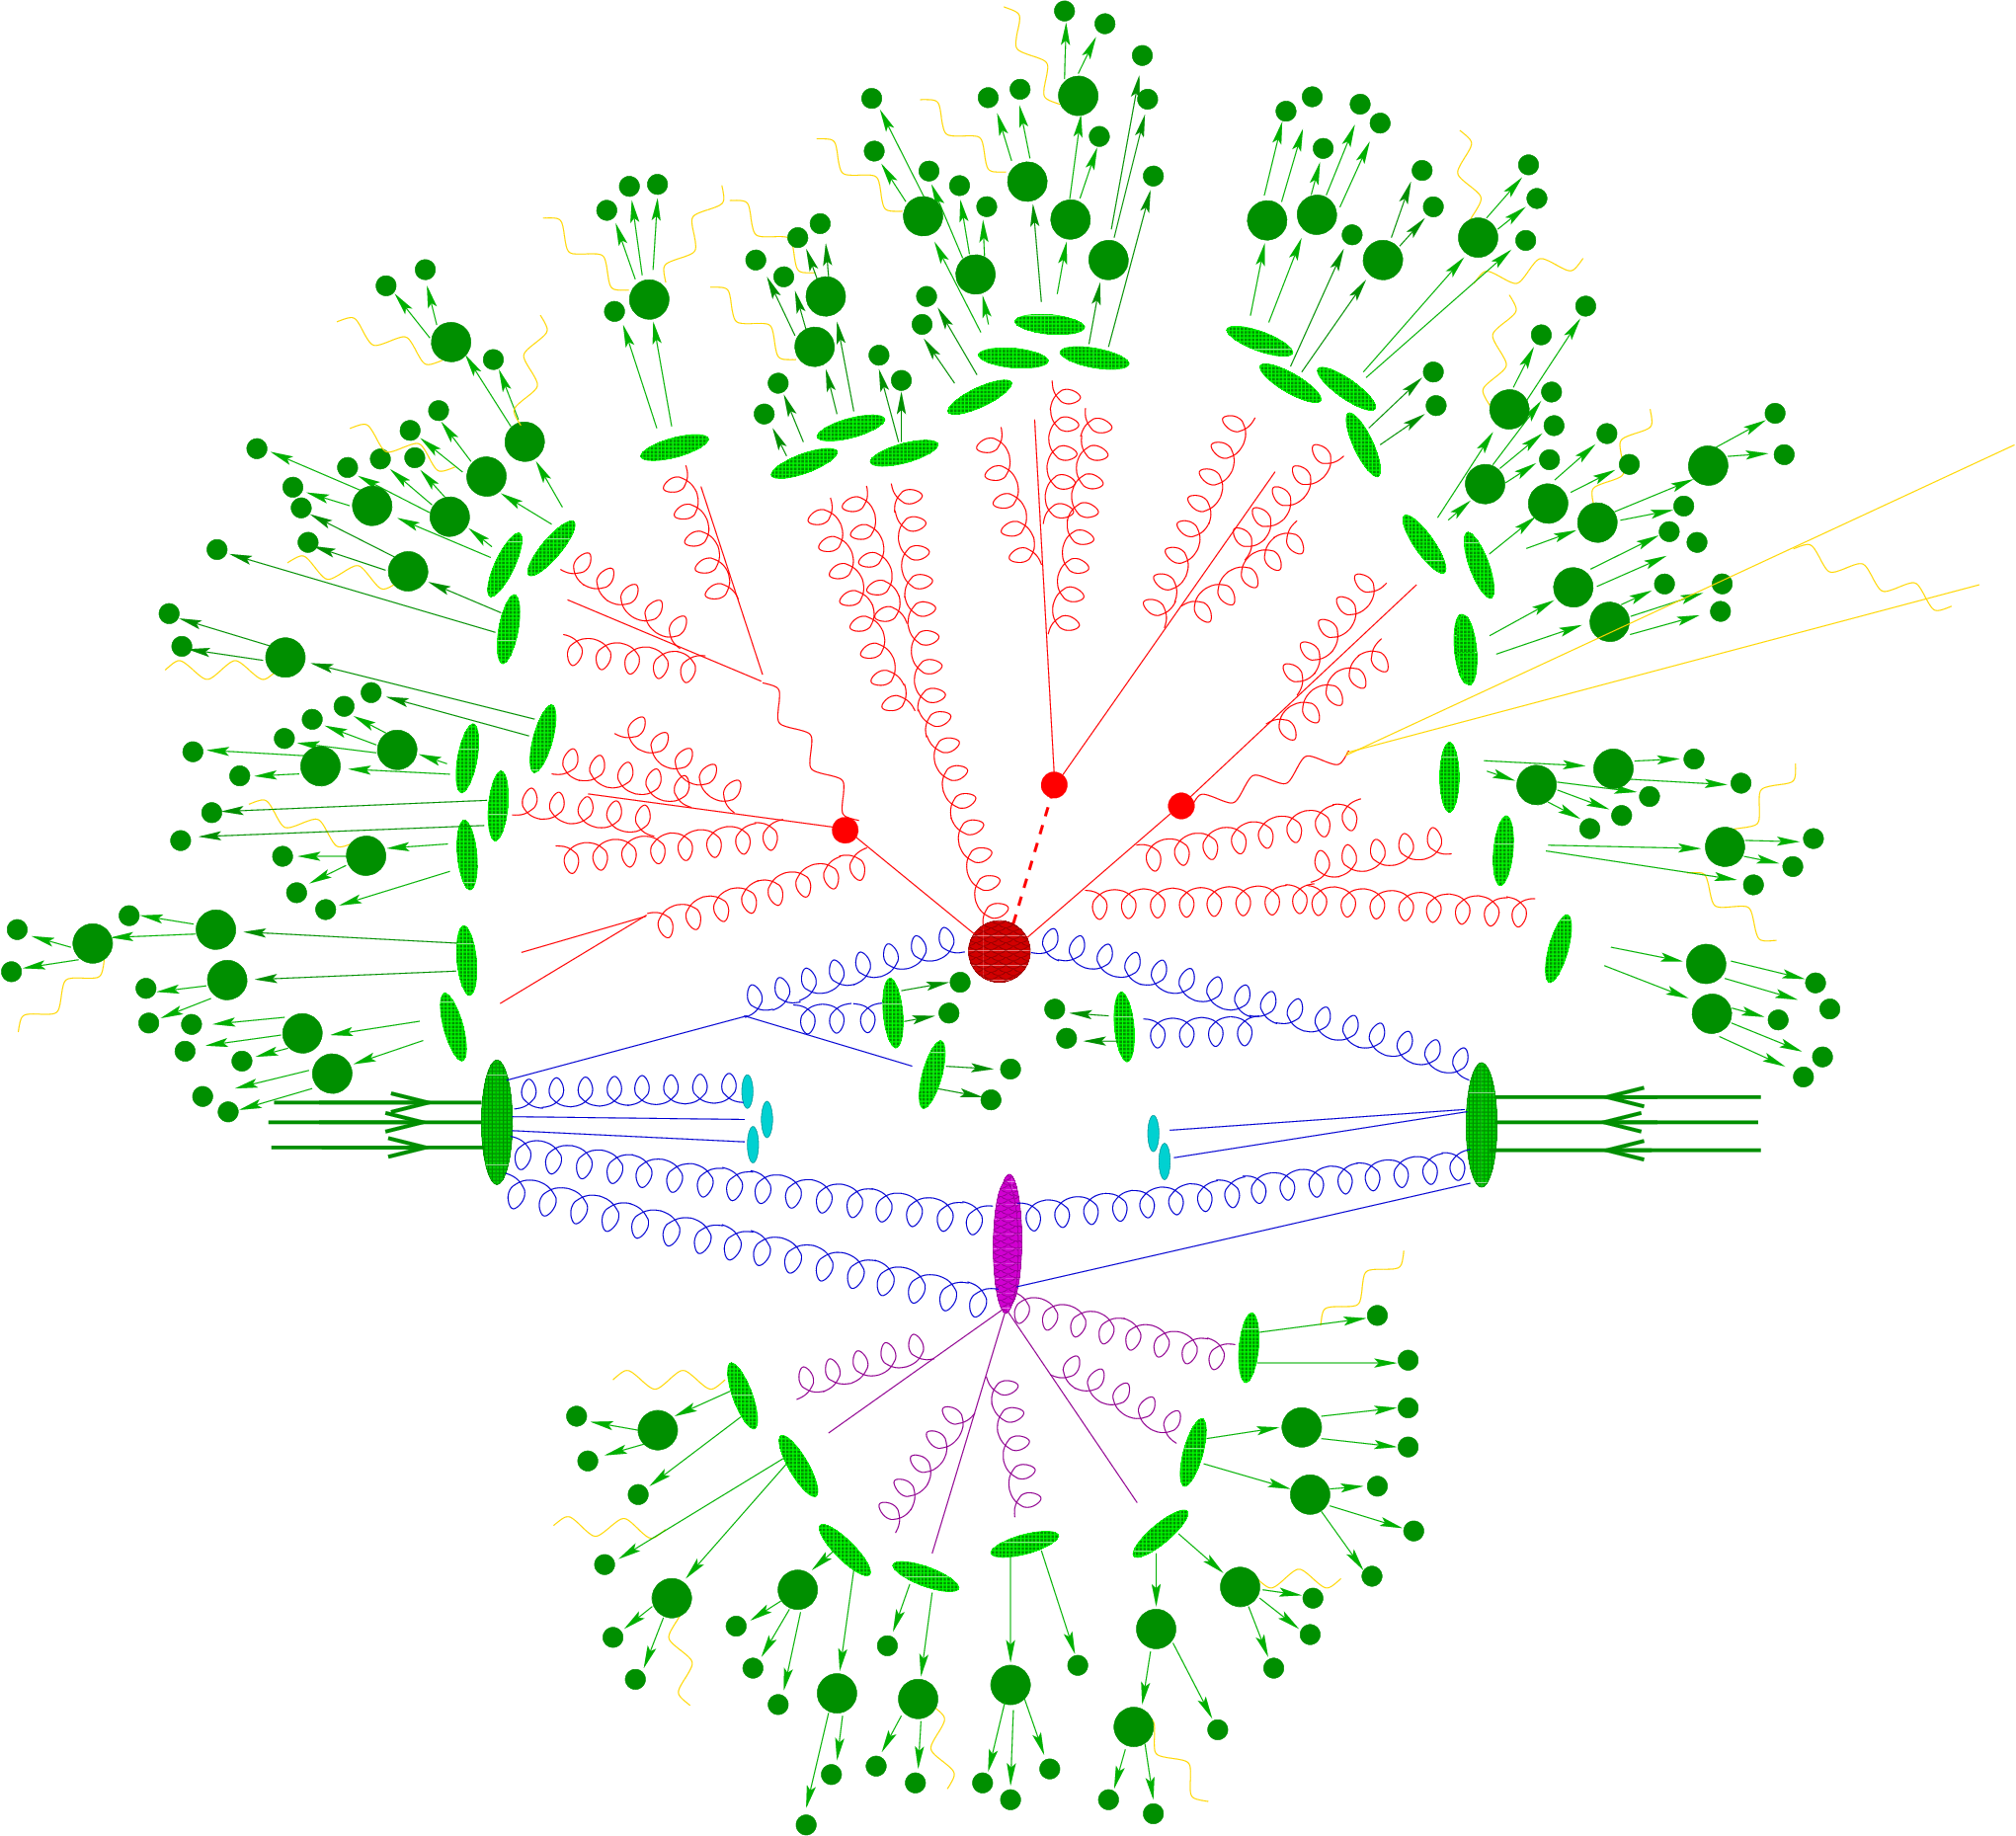
\includegraphics[width=.9\textwidth]{event.png} 
 \caption{Illustration of an event showing the hard scattering, parton shower, hadronisation, and underlying event. Figure taken from~\cite{Hoche:2014rga}.}
 \label{fig:event}
\end{figure}

\begin{itemize}
 \item[] \textbf{Hard scattering}\\
 In the hard interaction, two partons of the colliding protons, will interact with a certain probability at a given momentum transfer. This is parametrized by the \acp{PDF} $f(x, Q^2)$, were $x$ is the proton's momentum fraction and $Q^2$ is the momentum transfer scale. Experimentally determined \acp{PDF} are available from various groups, including e.g. CTEQ~\cite{Pumplin:2002vw}, MRST/MSTW~\cite{Martin:2009iq}, and NNPDF~\cite{Ball:2014uwa}. An example of such \acp{PDF} obtained by the NNPDF group is shown in Figure~\ref{fig:pdf}. This figure shows that the valence quarks in the proton, namely the up and down quarks it is made of, have a larger momentum fraction than the remaining sea quarks, which appear as virtual quark-antiquark pairs forming from gluons and annihilating again. The \acp{PDF} are then convoluted with the matrix element of the hard scattering, which is the process of interest where the two colliding partons create high-energetic final state particles. This is done using an event generator, such as \textsc{MadGraph5\_}a\textsc{MC@NLO}~\cite{Alwall:2014hca} and \textsc{PowHeg}~\cite{Frixione:2007vw}. With \textsc{MadGraph5\_}a\textsc{MC@NLO} the matrix element can for many processes be calculated at tree-level or \ac{LO}, and since the addition of a\textsc{MC@NLO} at \ac{NLO} as well. This generator was used to produce most of the background processes for the Monojet analysis detailed in Chapter~\ref{ch:monojet} and for the \ac{SIMP} signal used in Chapter~\ref{ch:SIMPs}. \textsc{PowHeg} is able to generate events using \ac{NLO} computations, but only for a relatively limited number of physics processes. This generator was used to produce the monojet signal samples and the background processes from single-top production. Since \ac{NLO} calculations are more time-consuming, one can instead use the less precise method of scaling a \ac{LO} cross section to the \ac{NLO} level by using a so-called k-factor, defined as the ratio of the \ac{NLO} and \ac{LO} cross sections. However, these k-factors often need to be determined as a function of the relevant kinematic variables as they depend on the kinematic phase space and the probed energy scale.

\begin{figure}[ht]
  \centering
 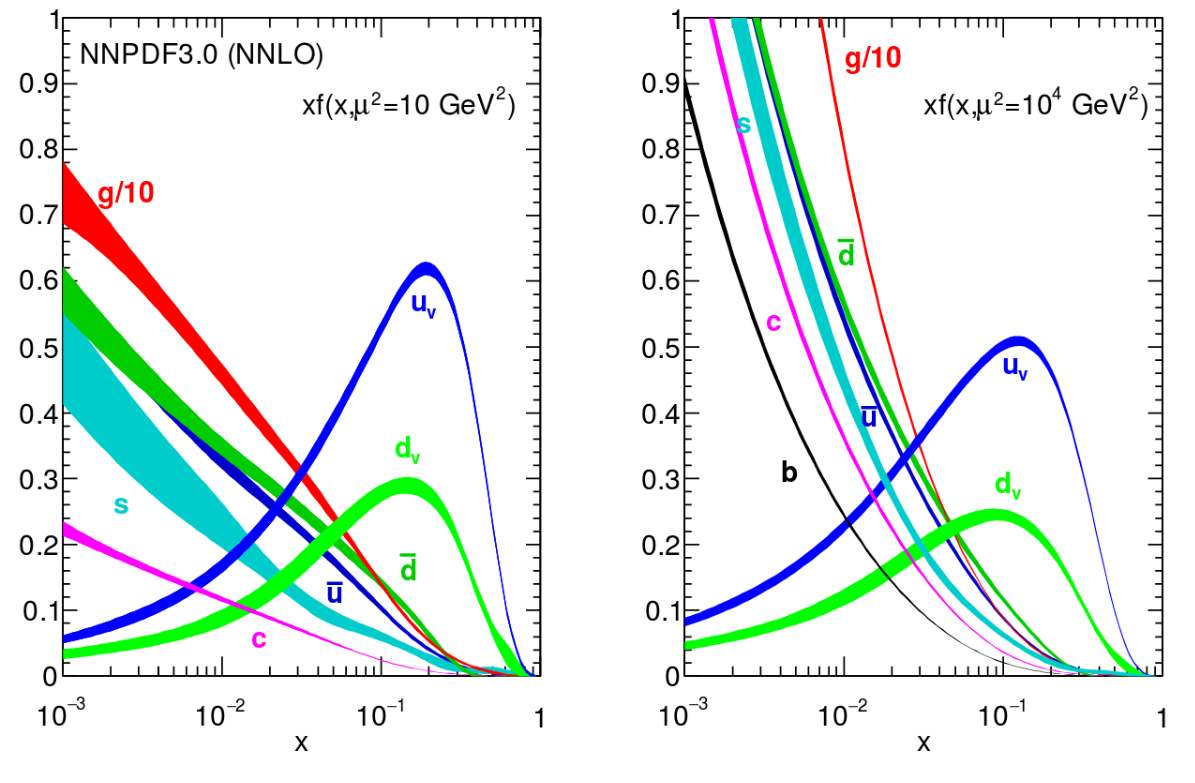
\includegraphics[width=.75\textwidth]{pdf.png} 
 \caption{The parton distribution functions multiplied by the momentum fraction $x$ at energy scales $Q^2 = \SI{10}{GeV^2}$ (left) and $Q^2 = \SI{10000}{GeV^2}$ (right), obtained in the NNLO NNPDF 3.0 global analysis. Figures taken from~\cite{Ball:2014uwa}.}
 \label{fig:pdf}
\end{figure}

 \item[] \textbf{Parton showering}\\
Since the colliding partons have a colour charge, the hard scattering will be accompanied by a cascade of radiation from \acs{QCD} processes. The partons will for example radiate soft gluons or split into two collinear partons. This radiation can originate from the incoming partons, which is referred to as \ac{ISR}, or the outgoing partons in the final state, the so-called \ac{FSR}. The perturbative evolution of the cascade can be modelled using the DGLAP (Dokshitzer-Gribov-Lipatov-Altarelli-Parisi) equations~\cite{Gribov:1972ri, Dokshitzer:1977sg, Altarelli:1977zs}. These equations describe the time evolution of the probability of a `mother' parton to split into `daughter' partons at an energy scale $Q^2$. The momentum of the mother is then divided among the daughter partons, which can in turn split into other partons at a lower $Q^2$ scale. The cascade continues down to an energy scale $\Lambda_{QCD}$ where the strong interaction becomes non-perturbative. The resulting number of jets can vary depending on the modelled process.
% , as shown in Figure~\ref{fig:njets}. {\color{red}Still need to describe figure, but it shows the opposite as expected for vector and scalar}
% 
% \begin{figure}[ht]
%   \centering
%  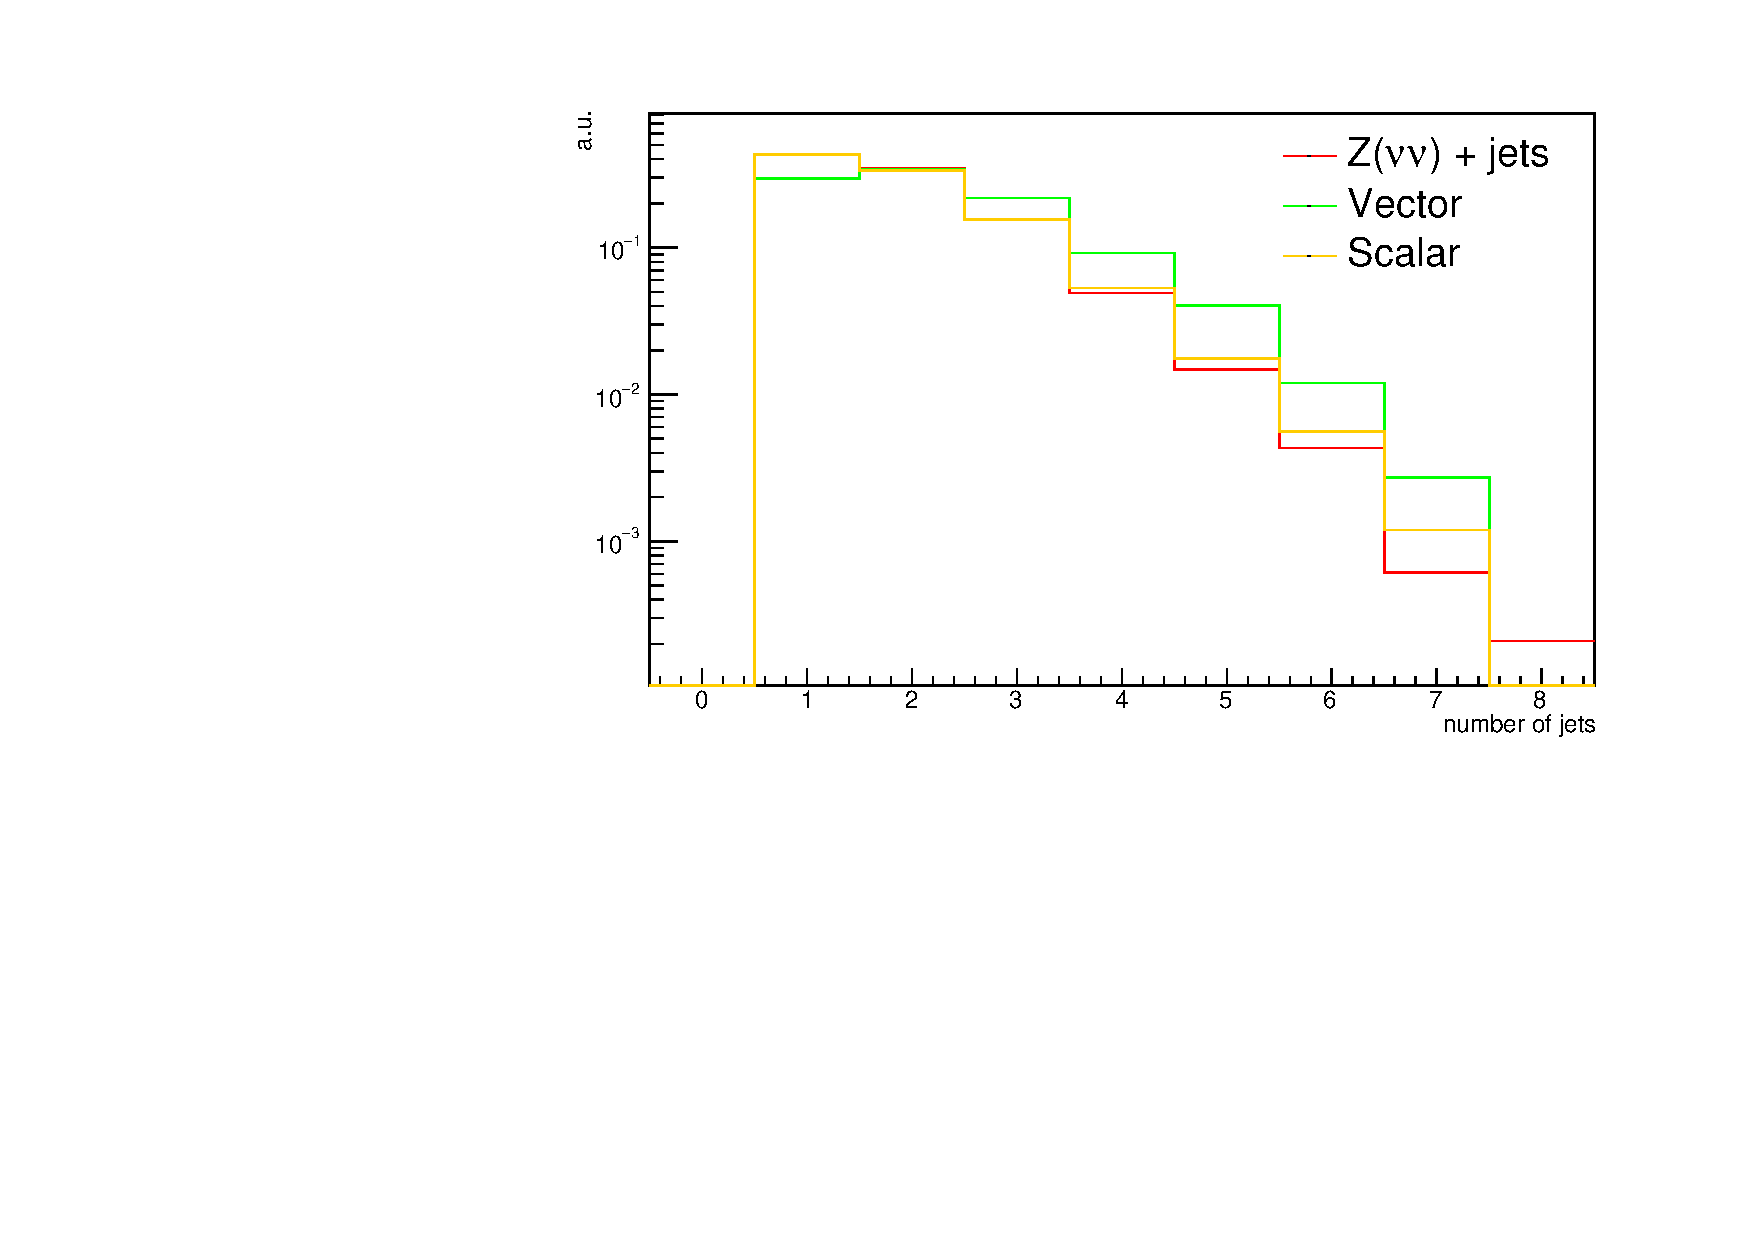
\includegraphics[width=.7\textwidth]{njets.pdf} 
%  \caption{.}
%  \label{fig:njets}
% \end{figure}

\item[] \textbf{Hadronisation}\\
The next step after the showering is the hadronisation of the coloured particles produced in the parton shower, transforming them into colour-neutral hadrons. Since this happens at low energy scales where the perturbative approach of \acs{QCD} is not valid, phenomenological models have to be used. For most of the processes considered in this thesis, the showering and hadronisation is done with \textsc{Pythia 8}~\cite{Sjostrand:2006za}, using a standard set of parameters which were tuned to reproduce the experimental data. In \textsc{Pythia}, the string Lund model~\cite{Andersson:1983ia} is used, based on string fragmentation. This model starts from the idea of a string connecting a quark $q$ and an antiquark $\bar{q}$, following the assumption of linear confinement. As the two quarks move away from each other, the string stretches and the potential energy stored in the string increases. The increase in potential energy is assumed to be proportional to the distance between the quarks. When the energy becomes sufficient to produce a new pair of quarks $q'\bar{q}'$ with mass $m$, the string breaks and the original quark pair is split into two new pairs, $q\bar{q}'$ and $q'\bar{q}$. If the invariant mass of the new strings is large enough, the same process is repeated, leading to a new break-up. This procedure continues until only colour-neutral hadrons with an on-shell mass remain.

\item[] \textbf{Additional activity in the event}\\
In addition to \ac{ISR} and \ac{FSR}, also beam remnants and multiple parton interactions give rise to additional activity in the event, referred to as the underlying event. After the partons participating in the hard scattering are extracted, the remainder of the protons have a non-zero colour charge. The creation of additional hadrons during the hadronisation is therefore possible. Multiple parton interactions represent additional interactions which can take place between other incoming partons. As the probability for an additional hard interaction to occur is rather small, the activity from multiple parton interaction is typically much less energetic than the hard interaction, producing mostly low energetic hadrons. Finally, additional collisions between other protons in the same bunch crossing, or from a previous or future bunch crossing, respectively referred to as in-time and out-of-time pileup, add extra activity in the event. The pileup distribution is for example shown in Figure~\ref{fig:pileup} for QCD dijet events recorded in 2016, and is compared to simulated QCD events. This shows that there were about $20$ collisions per bunch crossing on average. Typically, the simulation does not completely agree with the data and needs to be reweighted in order to match the data.

\begin{figure}[ht]
  \centering
 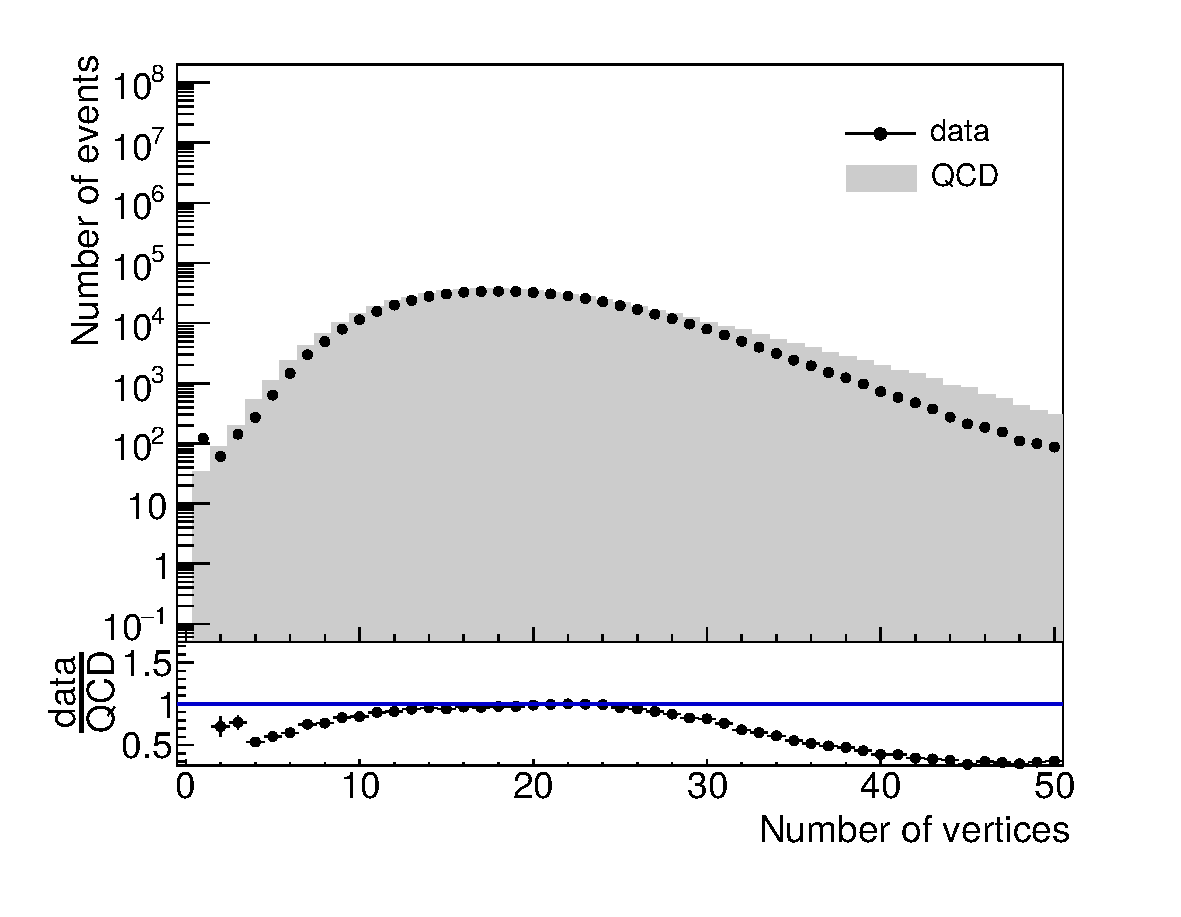
\includegraphics[width=.75\textwidth]{pileup.pdf} 
 \caption{The distribution of the number of vertices for \ac{QCD} dijet events recorded in 2016 compared to simulated \ac{QCD} events.}
 \label{fig:pileup}
\end{figure}
 \end{itemize}

\subsection{Generation of the monojet signals}
\label{sec:monojet_sim}

In the monojet analysis, the simplified models described in Section~\ref{sec:monojet_models} are considered. The used signal samples were generated with \textsc{PowHeg}, which can generate \ac{NLO} vector and axial-vector mediator production and \ac{LO} scalar and pseudoscalar production. The samples were also produced at \ac{LO} with MCFM~\cite{Campbell:2010ff} as a cross check. The scanned mediator masses are $m_{\phi} = 10, 20, 50, 100, 200, 300, 500,$ $ 1000, 2000,$ \SI{10000}{GeV}, for dark matter masses of $m_{\chi} = 1, 10, 50, 100, 150, 500, \SI{1000}{GeV}$, with $m_{\chi} \leq m_{\phi}$.

\subsection{Generation of the SIMP signal}
\label{sec:simp_sim}

For the generation of the \ac{SIMP} signal, the model Lagrangian given in equation~\ref{eq:SIMP_lagrangian} is implemented in \textsc{FeynRules 2.0}~\cite{Alloul:2013bka}. The matrix element is then calculated at \ac{LO} and events are generated using \textsc{Madgraph 5}. The subsequent parton shower and hadronisation is done with \textsc{Pythia 8}, using tune CUEP8M1. Several samples were produced, with \ac{SIMP} masses $m_{\chi} = 1, 10, 100, 200, 400, 700,$ \SI{1000}{GeV}. The interaction strength is assumed to be the same as the standard hadronic interaction $\sigma_{had} \approx \SI{40}{mb}$, and is not varied. A study using an interaction strength of $0.1\,\sigma_{had}$ can be found in~\cite{Daci:2015hca}, which shows that the \ac{SIMP} interacts later in the calorimeter and only a part of its energy is deposited in the detector. In this case, the designed analysis would still be sensitive to the scenarios with a low \ac{SIMP} mass. However, for even weaker interaction strengths the signal would completely disappear, which would result in a missing energy signature, such as the one considered in the monojet analysis. As a result, only a small window of interaction cross sections can be covered by the considered signature. The productions cross sections for the considered scenarios are given in Table~\ref{tab:signal_samples}. 

\begin{table}[ht]
  \centering
\caption{Production cross section for each \ac{SIMP} mass, after $|\eta_{\chi}| < 2.5$ and $p_{\rm T}^{\chi} > 200$ GeV generator level cuts.}
\begin{tabular}{| c | l |}
\hline
$m_\chi$ [GeV] & $\sigma_{\bar{\chi}\chi}$ [pb] \\
\hline
    1 &  4.46 \\
  10 &   4.40  \\
  100 &  2.55  \\
  200 &   0.790  \\
  400 &   0.0743   \\
  700 &   0.00485  \\
1000 &   0.000571  \\
\hline
\end{tabular}
\label{tab:signal_samples}
\end{table}

\section{Detector simulation}
\label{sec:sim}

After being generated, the collision events are passed on to the \ac{CMS} detector simulation, which is based on the \textsc{Geant 4}~\cite{Allison:2006ve} simulation toolkit. This toolkit provides a description of the interaction between particles and the detector material, including effects such as bremsstrahlung of charged particles, photon conversions, energy loss of charged particles by ionization, and the showering of electrons, photons and hadrons in the calorimeters due to interaction with the material. The \ac{CMS} simulation package contains the geometry of the detector with all the sensitive layers designed to detect the traversing particles, as well as the dead material regions consisting of e.g. support structures, cables and cooling pipes. A precise map of the magnetic field is also included in order to simulate the curvature of the charged particles correctly.

Next, the impact of the detector, coming from the electronic response produced by the hits in the active detector material, the digitization, the data transmission, and any reconstruction performed in the electronics such as zero-suppression or cluster reconstruction, is simulated. In this way, an event content similar to the output of the real detector is obtained. At this point the effect of pileup is also included by adding detector hits of generated proton-proton interactions on top of the hits resulting from the main interaction. Most of the simulated event samples used in this thesis are processed using this detector simulation. However, the interaction of new particles that can arise from specific theory models is not always readily described in \textsc{Geant}. This is the case for the signal samples used in the analysis described in Chapter~\ref{ch:SIMPs}, so an additional step was needed in order to simulate \acfp{SIMP} in the \ac{CMS} detector, described in Section~\ref{sec:SIMPs}. 

\section{Event reconstruction}
\label{sec:reconstruction}

Once the detector response has been simulated, the obtained events can be reconstructed. The same method is applied for these simulated events and for data coming from the detector. First, the reconstruction of tracks is performed, with a specific track reconstruction for electrons and muons. Furthermore, the calorimeter deposits, generated by electrons, photons, and hadrons, are grouped into clusters. Additionally, the reconstruction is further improved by using the so-called \acf{PF} algorithm described in Section~\ref{sec:PF}. This algorithm greatly improves the performance for jet and hadronic $\tau$ decay reconstruction, missing transverse momentum determination, as well as electron and muon identification. Finally, the obtained \ac{PF} candidates are clustered into jets, and the missing transverse energy can be derived.

\subsection{Track and vertex reconstruction}
\label{sec:tracking}

The tracks of charged particles going through the \ac{CMS} tracker are reconstructed with an iterative tracking approach. This is used to cope with the high occupancy of hits and consequently high combinatorics. Additionally, the first iterations search for tracks with less possible combinations, such as tracks with many pixel hits or a high momentum. After every iteration, the hits associated with the found track are removed to reduce the combinatorics. Each iteration consists of four steps:
\begin{enumerate}
 \item \textbf{Seed generation.} In this first step hits are combined into seeds for the subsequent track finding. In the initial iterations pixel triplets are used, then pixel pairs together with a constraint on the origin of the trajectory based on the assumption that it originated near the beam spot, in order to take gaps or non-working modules into account. Next, mixed pixel/strip triplets are taken, and finally strip-only seeds are used. These additional iterations improve the acceptance in $p_T$ and in displacement with respect to the primary vertex.
 \item \textbf{Track finding}. The seeds are used as starting point for a Kalman filter algorithm. This method extrapolates the seed trajectory outward to the next layer, taking into account the presence of the magnetic field, potential energy loss and multiple scattering. If compatible hits are found in the next layer, the parameters of the trajectory are updated. This process continues until the outermost layer of the tracking system. Using this method, a given seed can generate multiple tracks, or different tracks can share hits. A trajectory cleaner therefore determines the fraction of hits the tracks have in common and discards the track with the lowest number of hits when there are too many shared hits. If both tracks have the same number of hits, the track with the largest $\chi^2$ value is removed.
 \item \textbf{Track fitting.} The track parameters are then refitted using a Kalman filter and smoother, taking all hits determined in the track finding step into account. This is done in order to find the optimal track parameters.
 \item \textbf{Track selection.} Finally, the tracks are selected based on quality requirements, such as the number of layers that have hits, the $\chi^2/$dof, and the distance to a primary vertex. This greatly reduces the fraction of reconstructed tracks that are fake.
\end{enumerate}

The performance of the track reconstruction is excellent, and a high track-finding efficiency is obtained~\cite{Chatrchyan:2014fea} while keeping the rate of fake tracks negligible. The highest tracking efficiency is obtained for muons, which traverse the full detector volume and have an improved momentum resolution at high $p_T$ due to tracking information from the muon detectors giving a long lever arm. For isolated muons with $p_T$ between 1 and \SI{100}{GeV} the tracking efficiency is higher than 99\% for the entire $\eta$ coverage of the tracker, as can be seen from the left plot in Figure~\ref{fig:eff_eta}. The $p_T$ resolution is about 2-3\% for a muon with $p_T = $ \SI{100}{GeV} up to $|\eta| < 1.6$, but worsens for higher pseudorapidities. Different types of particles interact differently with the detector material. Charged hadrons, for example, are also subject to elastic and inelastic nuclear interactions and have a tracking efficiency of 80-95\% depending on pseudorapidity and transverse momentum, as shown in the right plot of Figure~\ref{fig:eff_eta}.

\begin{figure}[ht]
  \centering
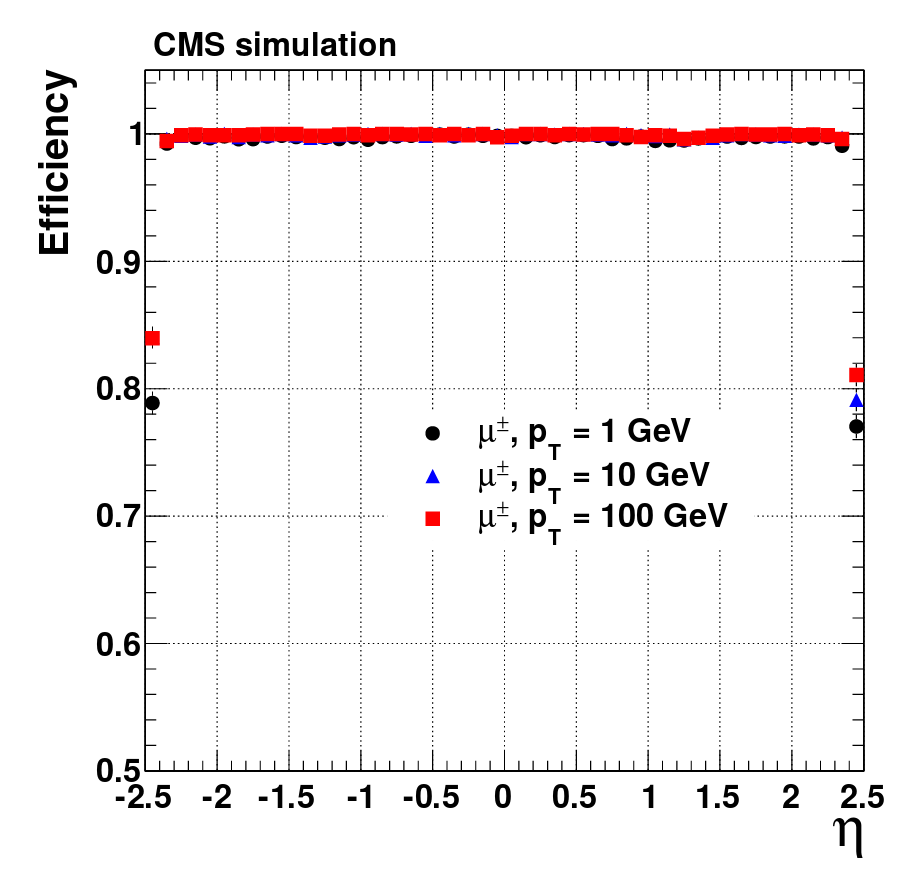
\includegraphics[width=.4\textwidth]{muon_eff_eta}\hspace{1cm}
 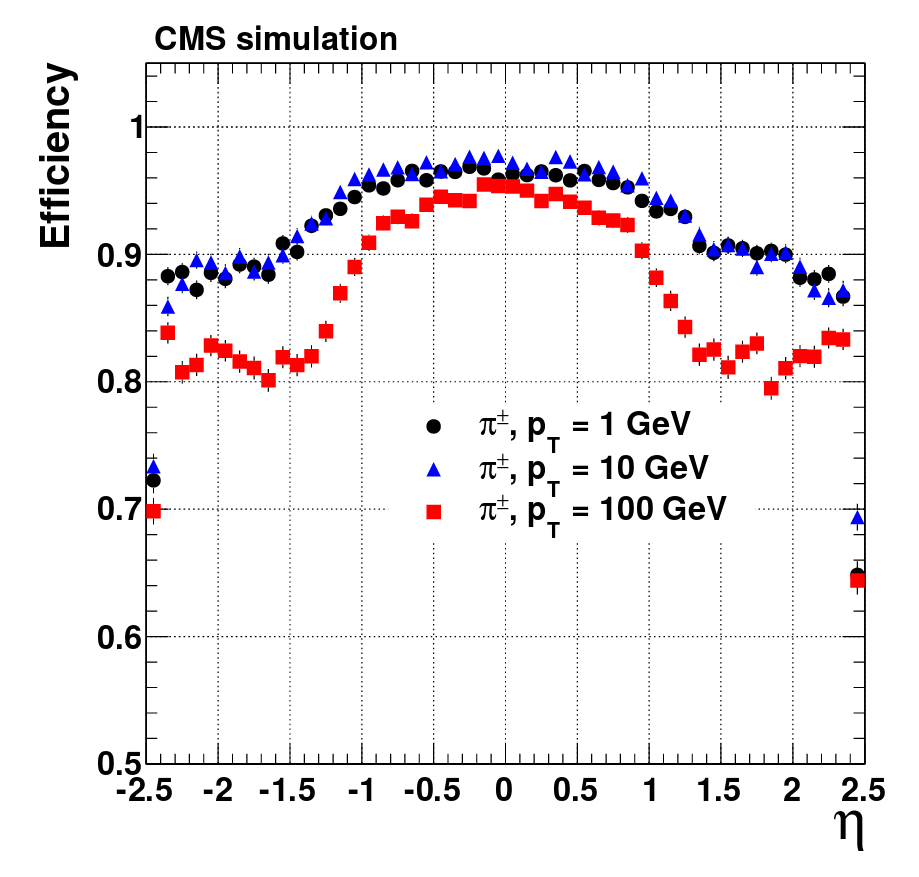
\includegraphics[width=.4\textwidth]{pion_eff_eta} 
 \caption{The muon efficiency (left) and pion efficiency (right) as a function of pseudorapidity, for multiple transverse momenta. Figures taken from~\cite{Chatrchyan:2014fea}}
 \label{fig:eff_eta}
\end{figure}

Finally, the primary vertices are reconstructed from the tracks. Since the collisions happen between bunches of protons, at the luminosities reached at the \ac{LHC} multiple protons will be colliding at the same time. The particles generated in these pileup interactions are all detected simultaneously and form a challenge to disentangle them from the particles coming from the to be studied interaction.

% The reconstruction is done in 2 steps: first the tracks that appear to originate from the same interaction vertex are clustered, then a fitting procedure computes the vertex parameters and assigns a weight to each associated track, reflecting the probability that it corresponds to the considered vertex. Figure~\ref{fig:PV} shows the reconstruction efficiency and the resolution of the primary vertex. The more tracks, the better the vertex is constrained and thus the better the resolution.

The reconstruction is performed as detailed in Section~9.4.1 of~\cite{CMSCollaboration:2015zni}, by first clustering the tracks based on their $z$ coordinate at the point of closest approach to the beam line. The vertex position is then estimated using an adaptive vertex fit~\cite{Fruhwirth:2007hz} with as input the collection of tracks that is expected to come from the same interaction. Next, the tracks originating from the same vertex are clustered into jets with the anti-$k_T$ algorithm described in Section~\ref{sec:jet_reconstruction} using a distance parameter of 0.4.

% \begin{figure}[ht]
%   \centering
% 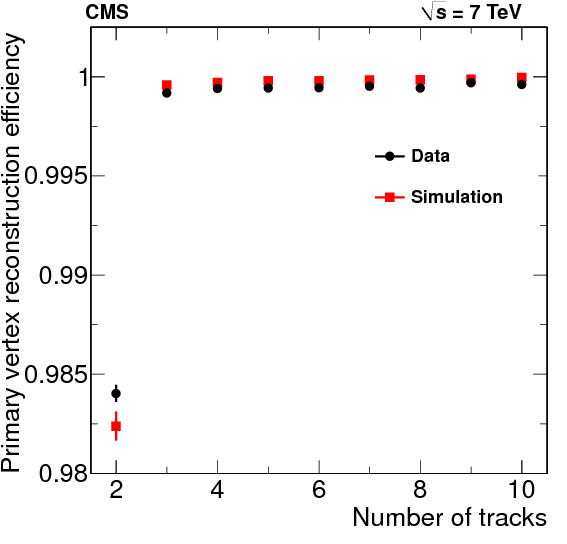
\includegraphics[width=.4\textwidth]{PV_eff}\hspace{1cm}
%  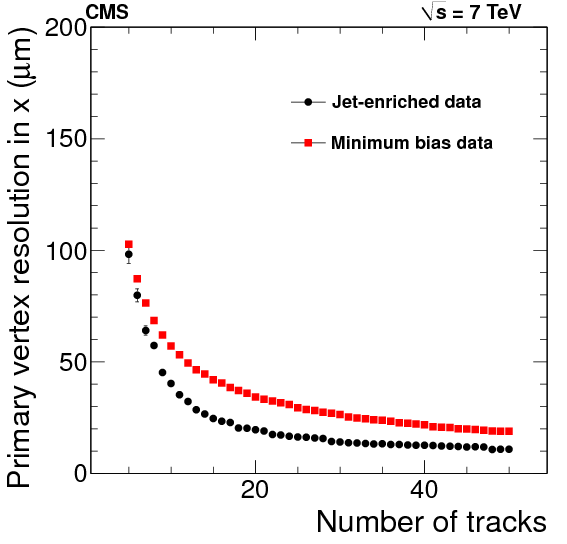
\includegraphics[width=.4\textwidth]{PV_res} 
%  \caption{The primary vertex reconstruction efficiency (left) and resolution (right) as a function of the number of tracks associated to it. Figures taken from~\cite{Chatrchyan:2014fea}}
%  \label{fig:PV}
% \end{figure}

The vertex with the highest $\sum p_T^2$ is chosen as primary vertex, where the sum runs over these reconstructed jets, as well as the remaining tracks associated to the vertex and the missing transverse momentum at this vertex, in order to take into account neutral particles.
%tracks associated to the vertex following the application of a deterministic annealing filter which assigns weights to sufficiently high-quality tracks that enter the vertex fit~\cite{Chatrchyan:2014fea}. 
While in events with jets many tens of high-momentum tracks can usually be associated to a primary vertex, thus making primary vertex finding almost fully efficient and pure, in the case of a pair of neutral jets, produced for example by \acp{SIMP}, this is not the case any more. The underlying event and potentially initial state \acs{QCD} radiation can still provide some tracks, but in extreme cases a wrong vertex is chosen, arising from a hard pileup collision.

\subsection{Electron and isolated photon reconstruction}
\label{sec:electron_reconstruction}

Electrons are reconstructed using information from both the tracker and the calorimeters. Due to the large amount of material present in the tracker, electrons will emit bremsstrahlung photons, and photons will often convert into $e^+e^-$ pairs, which can again radiate bremsstrahlung photons.

For electrons, a \ac{GSF}~\cite{Strandlie:2006gi} candidate is taken as starting point. This \ac{GSF} candidate is obtained using 2 different methods to reconstruct the electron track from the hits in the tracker, which should gather all radiated energy from the electron. First, the ECAL-based approach is used, grouping \ac{ECAL} clusters into superclusters. These superclusters collect the energy of the electron and the bremsstrahlung photons in a small $\eta$ window and a large $\phi$ window, taking the bending of the electron track in the magnetic field into account. The supercluster energy and position is then used to estimate the position of the corresponding hits in the tracker layers. Subsequently, the tracker-based approach is used to find electrons missed by the ECAL-based method. In this case, the tracks from the iterative tracking with transverse momentum larger than \SI{2}{GeV} are used. Additional requirements are placed on the number of hits and the $\chi^2$ of the fit, and the specific electron tracking is performed, using a \ac{GSF} fit, which is more adapted to electrons than the Kalman filter used in the iterative tracking, as it describes the energy loss in each tracker layer. The electron seeds obtained with both methods are merged and used as input for the full electron tracking. The obtained electron tracks are then linked to \ac{ECAL} clusters by the \ac{PF} algorithm, as described in Section~\ref{sec:PF}. In the case of isolated photons, a candidate is seeded from an \ac{ECAL} supercluster with transverse energy larger than \SI{10}{GeV} which is not linked to a \ac{GSF} track.

The total energy of the accumulated \ac{ECAL} clusters is corrected for the energy that was lost in the process of reconstruction, using analytical functions of the energy and pseudorapidity. The applied corrections can be as large as 25\%, at low transverse momentum and at $|\eta| = 1.5$, where the material density in the tracker is largest. The energy of the electron is then obtained from a combination of the corrected energy and the momentum of the \ac{GSF} track, while the direction of the electron is taken from the \ac{GSF} track. For photons, the corrected energy and the direction of the supercluster are used.
% 
%  while for photons the candidates must be isolated from other tracks and calorimeter clusters, and the energy distribution in the \ac{ECAL} and the ratio between the \ac{HCAL} and \ac{ECAL} energies must be compatible with the expectation from a photon shower.

\subsection{Electron and photon identification}
\label{sec:electron_ID}

In general, the electron and photon candidates must satisfy identification criteria to be retained. In the case of electrons two methods for identification are available: a cut-based identification or a multivariate boosted decision tree (BDT) combining fourteen variables including the amount of energy radiated and the ratio between the energies gathered in HCAL and ECAL. In the monojet analysis described in Chapter~\ref{ch:monojet}, the former is used. In this method, four different working points are defined, denoted as ``tight'', ``medium'', ``loose'', and ``veto'', with varying signal efficiency and background rejection. For the electron veto the loose selection is used, while a tight identification is required on one electron to select the events in the dielectron and single electron control regions.

\renewcommand{\arraystretch}{1.1}
\begin{table}[ht!]
\centering
\small
\caption{Loose and tight electron identification criteria. The isolation is computed in a cone of $\Delta R < 0.3$ around the electron.}
\begin{tabular}{|l|l|l||l|l|c|}
\hline
\multirow{2}{*}{variable}                             &  \multicolumn{2}{c||}{loose} &  \multicolumn{2}{c|}{tight} \\
\cline{2-5}
                                                            &  barrel        & endcaps  &  barrel  & endcaps\\
\hline
full 5x5 $\sigma_{i\eta i\eta}$                             & $< 0.0114  $     & $< 0.0352  $ & $< 0.0101  $     & $< 0.0279  $ \\
$|\Delta \eta_{in}|$                                        & $< 0.0152  $     & $< 0.0113  $ & $< 0.00926 $     & $< 0.00724 $ \\
$|\Delta \phi_{in}|$                                        & $< 0.216   $     & $< 0.237   $ & $< 0.0336  $     & $< 0.0918  $ \\
H/E                                                         & $< 0.181   $     & $< 0.116   $ & $< 0.0597  $     & $< 0.0615  $ \\
relative isolation			                    & $< 0.126   $     & $< 0.144   $ & $< 0.0354  $     & $< 0.0646  $ \\
$|1/E - 1/p|\ [\mathrm{GeV}^{-1}]$                          & $< 0.207   $     & $< 0.174   $ & $< 0.012   $     & $< 0.00999 $ \\
$|\mathrm{d_{xy}(vtx)}|$ [cm]                               & $< 0.0564  $     & $< 0.222   $ & $< 0.0111  $     & $< 0.0351  $ \\
$|\mathrm{d_{z}(vtx)}|$ [cm]                                & $< 0.472   $     & $< 0.921   $ & $< 0.0466  $     & $< 0.417   $ \\
expected inner missing hits                                 & $\leq 2$         & $\leq 3$     & $\leq 2$           & $\leq 1$   \\
pass conversion veto                                        & yes              & yes          & yes              & yes        \\
\hline
\end{tabular}
\label{tab:ElectronID}
\end{table}

Similarly, for the photons, both a cut-based identification and a multivariate analysis can be used. Both for the monojet and the \ac{SIMP} analysis, described in Chapters~\ref{ch:monojet} and \ref{ch:SIMPs}, the cut-based identification is used. Three standard working points are provided, denoted as ``loose'', ``medium'', and ``tight'', with an average efficiency of 70\%, 80\%, and 90\%, respectively. In both analyses, the loose identification is used for the photon veto. In the \ac{SIMP} analysis, the event is only rejected when the identified photon is within a cone of $\Delta R < 0.1$ of one of the two leading jets. Additionally, the photon veto is extended to reject events containing jets with a large photon energy fraction and unidentified photons. This happens for instance when there is a photon conversion in the tracker. The event is therefore rejected when the jet photon energy fraction is larger than 0.8, the photon is not identified by the loose criteria, and a conversion is matched to the photon within $\Delta R < 0.2$ and has $p_{T,conv} / p_{T,\gamma} > 0.3$. Lastly, the two jets are also required to have a neutral electromagnetic energy fraction lower than 0.9, corresponding to one of the standard tight jet identification requirements mentioned in Section~\ref{sec:jet_reconstruction}. Finally, the monojet analysis uses a photon + jets control region as well. These events are selected by applying the tight photon identification.


\renewcommand{\arraystretch}{1.1}
\begin{table}[ht!]
\centering
\footnotesize
\caption{Loose and tight photon identification criteria. The isolation is computed in a cone of $\Delta R < 0.3$ around the photon.}
\begin{tabular}{|l|l|l||l|c|}
\hline
\multirow{2}{*}{variable}                             &  \multicolumn{2}{c||}{loose} & tight \\
\cline{2-4}
                                                            &  barrel        & endcaps  &  barrel  \\
\hline
full 5x5 $\sigma_{i\eta i\eta}$            & $< 0.0102$                                                  & $< 0.0274$    & $< 0.0102$     \\
H/E                                        & $< 0.05$                                                    & $< 0.05$     & $< 0.05$      \\
charged hadron                   & \multirow{2}{*}{$< 3.32$}  & \multirow{2}{*}{$< 1.97$}    & \multirow{2}{*}{$< 1.37$}    \\
 isolation        &     &      &   \\
neutral hadron  & $< 1.92 + 0.014\times p_T$ & $< 11.86 + 0.0139\times p_T$ & $< 1.06 + 0.014\times p_T$  \\
isolation          & $\quad +1.9\times 10^{-5} \times {p_T}^2$  & $\quad +2.5\times 10^{-5} \times {p_T}^2$ & $\quad +1.9\times 10^{-5} \times {p_T}^2$ \\
photon isolation                           & $< 0.81 + 0.0053\times p_T$                                 & $< 0.83 + 0.0034\times p_T$ & $< 0.28 + 0.0053\times p_T$   \\
conversion safe             & \multirow{2}{*}{yes}                                                         & \multirow{2}{*}{yes}        & \multirow{2}{*}{yes}       \\
electron veto              &      &   &  \\
\hline
\end{tabular}
\label{tab:PhotonID}
\end{table}

\subsection{Muon reconstruction}
\label{sec:muon_reconstruction}

Muon tracking is performed using 2 complementary approaches. The first method starts from standalone muons, which are reconstructed from hits in the muon detectors only using pattern recognition. The standalone muons are then matched to tracks in the tracker, and the hits are combined to form a global muon track. This global muon fit improves the momentum resolution compared to the tracker-only fit at muon momenta larger than \SI{200}{GeV}.

For momenta below \SI{10}{GeV}, muons often fail the global muon conditions which require the muon to penetrate through more than one muon detector plane, due to the large multiple scattering in the return yoke. In this case, tracker-only muon reconstruction is more efficient since it only requires one muon segment. Each track in the tracker with a transverse momentum larger than \SI{0.5}{GeV} and a total momentum larger than \SI{2.5}{GeV} is therefore extrapolated to the muon system and if at least one matching track segment is found, it is retained as muon candidate.

Within the geometrical acceptance of the muon system about 99\% of the muons are reconstructed, either as global muon or as tracker muon and frequently as both. Global and tracker muons that share the same track inside the tracker are merged into a single candidate. Muons that are only reconstructed as standalone muons have a worse momentum resolution compared to the global and tracker muons. These standalone muons are however only considered in the further reconstruction when the fit is of high quality and is associated with a large number of hits in the muon system.

Charged hadrons can be misreconstructed as muons if e.g. a part of the hadron shower reaches the muon system. In order to improve the muon identification, the \ac{PF} muon identification algorithm described in Section~\ref{sec:PF} also matches energy deposits in the \ac{ECAL} and \ac{HCAL} with the muon track.

\subsection{Muon identification}
\label{sec:muonID}

When using muons for physics analysis, some identification criteria are generally applied in order to ensure the quality of the muons. There are several standard levels of identification, denoted as ``tight'', ``medium'', and ``loose'', which provide a trade-off between muon identification efficiency and misidentification. In general, the tight and loose identification are the most widely used identification criteria.

The loose identification only requires the muons to be either global or tracker-only muons, and to be identified by the \ac{PF} algorithm as a muon. As a result, it is highly efficient for both prompt muons and muons from quark decays. In analyses with prompt muons, this identification is therefore often complemented by an impact parameter cut, associating the muon to the primary vertex.

For the tight identification, the muon is required to be a global muon and to be identified by the \ac{PF} algorithm as a muon. The normalized $\chi^2$ of the global muon track fit should be smaller than 10 to suppress hadronic punch through and muons from hadron decays in flight. To further suppress these contributions at least one muon chamber hit should be included in the global muon track fit and muon segments should be found in at least two muon stations. Cosmic muons and tracks from pileup are suppressed by requiring the tracker track to have $|d_{xy}| < \SI{2}{mm}$ and $|d_z| < \SI{5}{mm}$, with $d_{xy}$ the traverse impact parameter and $d_z$ the longitudinal distance with respect to the primary vertex. Finally, at least one pixel hit is required, as well as hits in at least 5 tracker layers, in order to ensure a good $p_T$ measurement.

In the case of the monojet analysis described in Chapter~\ref{ch:monojet}, the loose muon identification is used to select muons for the muon veto. An additional isolation cut of 0.2 is applied in order to reject muons inside jets. The isolation value is computed as the sum of the transverse momenta of all charged hadrons associated to the primary vertex, neutral hadrons, and photons in a cone of $\Delta R < 0.4$ around the muon, relative to the $p_T$ of the muon. The tight muon identification is used as well, to select events in the dimuon and single muon control regions. 

\subsection{Particle flow}
\label{sec:PF}

The \acf{PF} algorithm~\cite{CMS-PRF-14-001} reconstructs so-called particle flow candidates by combining information from all different \ac{CMS} subdetectors, linking different elements, such as tracks in the tracker, calorimeter clusters, and muon tracks. A global picture of the event is thus formed, where each particle is uniquely identified. The obtained collection of particle candidates is subsequently used to reconstruct jets and tau leptons, and to determine the missing transverse momentum.

In a first step, the \ac{PF} algorithm identifies charged particle tracks, as defined in Section~\ref{sec:tracking} for all tracks, and in Sections~\ref{sec:electron_reconstruction} and \ref{sec:muon_reconstruction} for electron and muon tracks in particular. At the same time, the calorimeter clusters are reconstructed with a clustering algorithm designed specifically for the \ac{PF} event reconstruction. In this algorithm, cluster seeds are first identified as local energy maxima with respect to the four or eight closest cells, if the energy deposited in the cell is above a given seed threshold. The clusters are then formed by accumulating neighbouring cells with an energy above a given cell threshold, suppressing noise.

The \ac{PF} elements in the different subdetectors are then connected by a link algorithm which avoids any double counting. The link algorithm produces blocks of associated elements, quantifying the quality of the link by defining a geometrical distance between the elements. When an element is linked to multiple other elements, only the link with the shortest distance is kept. More precisely, a link between a track in the tracker and a calorimeter cluster is made by extrapolating it from the last hit in the tracker to the calorimeters. The distance between the position of the extrapolated track and the cluster in the ($\eta$, $\phi$) plane is then used to define the link distance. At the interaction points between the track and the tracker layers, tangents to the \ac{GSF} tracks are extrapolated to the \ac{ECAL} in order to collect the energy of photons radiated by electron bremsstrahlung. A dedicated conversion finder was also developed to identify bremsstrahlung and prompt photon conversions into $e^+e^-$ pairs. Links between calorimeter clusters are established outside of the tracker acceptance, or between the preshower and \ac{ECAL} clusters in the preshower acceptance. In this case the link distance is also defined as the distance between the position of the clusters. Charged particle tracks can also be linked by a common secondary vertex. Finally, the \ac{PF} muon identification algorithm associates the muon tracks to the muon energy deposits in the \ac{ECAL} and \ac{HCAL}, to improve the muon identification performance.

In a next step, the \ac{PF} blocks obtained by linking the multiple \ac{PF} elements, are classified as muons, electrons, or isolated photons. The corresponding elements are then excluded from further consideration. Once electrons, muons, and isolated photons have been identified, the remaining elements are identified as charged hadrons, neutral hadrons, or photons produced in jets. Within the tracker acceptance, the \ac{ECAL} clusters not linked to any track are classified as photons, while the clusters in the \ac{HCAL} without a matched track are labelled as neutral hadrons. Outside of the tracker acceptance, charged and neutral hadrons can not be distinguished. \ac{ECAL} clusters linked to an \ac{HCAL} cluster are then assumed to arise from the same hadron shower, and the estimated energy for these particles is the sum of the energy deposited in the \ac{ECAL} and the \ac{HCAL}. The \ac{ECAL} clusters that are not linked to an \ac{HCAL} cluster are classified as photons.

% how does a photon shower differ from an electron shower? 
% 
% what about converted photons? 
% 
\subsection{Jet reconstruction}
\label{sec:jet_reconstruction}

% line 7: you are only using PF and CALO jets maybe, but there are also track jets.
% 
% line 37/38: I don't really understand the concept of the jet area from this. This is not the same as the area that comes from the e.g. anti-kT algorithm but something else?

Jets are reconstructed with the anti-$k_T$ algorithm~\cite{1126-6708-2008-04-063}, which clusters either the generated particles from event simulation, or the particles reconstructed by the \ac{PF} algorithm (\ac{PF} jets), or the energy deposits in the calorimeters (Calo jets). This procedure takes into account the transverse momentum $p_T$, also called $k_T$, of the particles and the distance between particles, defined as \begin{equation}                                                                                                                                                                                                                                                                                                     
 \Delta R_{ij} = \sqrt{(\eta_i - \eta_j)^2 + (\phi_i - \phi_j)^2}.                                                                                                                                                                                                                                                                                        \end{equation}
The strategy consists of the following steps:
\begin{enumerate}
 \item For every pair of particles $i$ and $j$, a distance $d_{ij}$ defined as 
 \begin{equation}
  d_{ij} = \min\left(\frac{1}{p_{Ti}^2}, \frac{1}{p_{Tj}^2} \right)\frac{\Delta R_{ij}^2}{R^2}
 \end{equation}
 is calculated.
 \item For every particle $i$, a distance $d_{iB}$ to the beam pipe is calculated with
 \begin{equation}
  d_{iB} = 1/p_{Ti}^{2}.
 \end{equation}
 \item The minimum of $d_{ij}$ and $d_{iB}$ is then determined.
 \item If it is $d_{ij}$, particles $i$ and $j$ are recombined into a new particle by adding the four-momenta of the particles. If it is $d_{iB}$, particle $i$ is declared to be a jet and it is removed from the list of particles.
 \item This is repeated until no particles remain.
\end{enumerate}

In this clustering algorithm, the parameter $R$ determines what is called a jet. If a particle $i$ has no other particles within a distance $R$, $d_{iB}$ will be smaller than $d_{ij}$ and the particle will become a jet. A consequence of this is that an arbitrarily soft particle can become a jet, and therefore a minimum transverse momentum for a jet to be of interest is defined.

The anti-$k_T$ algorithm favours clustering around hard particles, and the jets then grow outward from this seed. This gives rise to circular jets, with a cone size that is proportional to $R$. Since it still involves a combination of energy and angle in the distance measure, this is a collinear-safe growth, meaning that the jet will not change when one of the particles of the jet is split collinearly. This algorithm is also infrared-safe, i.e. the same set of jets is obtained when soft particles are emitted.

A reliable determination of the jet energy is not straightforward, since many effects can distort the energy estimation, such as the calorimeter response, the limited particle reconstruction efficiency, the underlying event, the pileup, and the charged particles bending out of the jet cone due to the strong magnetic field. The pileup is mitigated by applying \ac{CHS}, which consists of removing charged hadrons associated with vertices other than the primary vertex from the list of \ac{PF} candidates. Additionally, the jet energy is corrected using a factorised approach, as illustrated in Figure~\ref{fig:JEC}, with the following steps:
\begin{itemize}
 \item \textbf{Pileup correction (L1).} The first level of jet energy corrections is applied event-by-event and jet-by-jet, and is determined from simulation. It is dependent on the pseudorapidity and transverse momentum of the jet, the average $p_T$ density in the event, and the effective jet area. This effective area is determined by injecting a large number of very soft particles in the event before the jet clustering. The spread of the soft particles in each jet then defines the jet area. When these corrections are applied on data, residual corrections are also applied to take into account the difference between the simulated events and the data.
 
 \item \textbf{Relative $\eta$ and absolute $p_T$ corrections (L2L3).} These corrections are also obtained from simulations and correct for the non-uniform response of the calorimeters in $\eta$ and $p_T$. They are determined by comparing the reconstructed $p_T$ to the one obtained from the jets built from the generated particles. These corrections have the largest impact on the jet energy.
 
 \item \textbf{Residual $\eta$ and $p_T$ corrections (L2L3Residual).} Since the L2L3 correction is derived from simulation, additional residual corrections are needed in order to correct for the remaining small differences between the jet response in data and simulation. These corrections are typically of the order of a few percent.
\end{itemize}

\begin{figure}[ht]
  \centering
 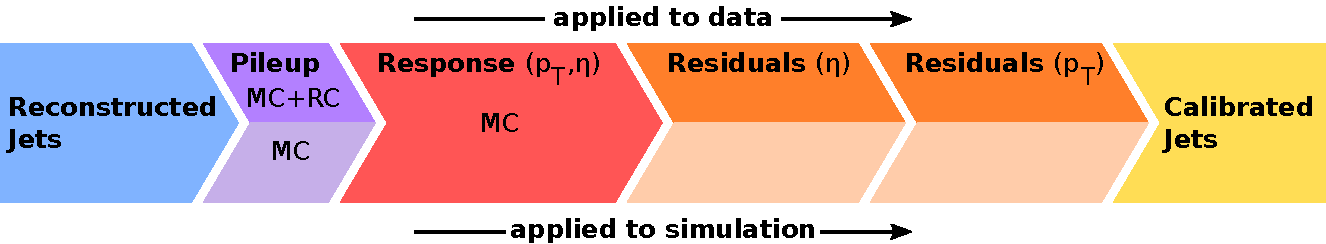
\includegraphics[width=.85\textwidth]{JEC.pdf} 
 \caption{Graphical overview of the factorised approach used at \ac{CMS} to apply jet energy corrections.}
 \label{fig:JEC}
\end{figure}

Optionally, a set of identification criteria are applied on the \ac{PF} jets. A jet is required to consist of at least two particles. For jets in the region $|\eta| < 2.7$, the fraction of energy coming from ether neutral hadrons or photons should not exceed 99\%. Additionally, for jets restricted to the tracker acceptance ($|\eta| < 2.4$), there should at least be some energy deposited in the \ac{HCAL}, the jet should contain 1 or more charged constituent, and the fraction of energy corresponding to electrons or photons should not exceed 99\%. 

Moreover, jets from pileup can be identified as well. This pileup jet identification relies on the topology of the jet shape which is used to disentangle jets coming from the overlap of multiple interaction and real hard jets, the object multiplicity, and the compatibility of the tracks in the jets with the primary vertex. This last property of pileup jets can evidently only be exploited for jets within the tracker acceptance.

Both jet and pileup jet identification are used in the monojet analysis described in Chapter~\ref{ch:monojet}. In the trackless jets analysis described in Chapter~\ref{ch:SIMPs} however, the full jet ID is not applied, since the requirements on e.g. the neutral hadronic energy fraction and the charged multiplicity would reject the signal events. Instead, only the requirement on the jet neutral electromagnetic energy fraction is applied, in order to reject photons.

\subsection{Identification of b-jets}
\label{sec:btagging}

For the identification of jets originating from $b$ quarks, the long lifetime of the B hadrons arising from the hadronisation of $b$ quarks is exploited. The B hadrons will therefore decay at a position that is displaced with respect to the primary interaction vertex. The b-jets can then be identified by looking for the presence of displaced tracks from which a secondary vertex may be reconstructed. Additionally, the B hadrons have a probability of 20\% to decay into muons or electrons. Consequently, the presence of these charged leptons can be used as well for b-jet identification techniques.

Within the \ac{CMS} collaboration, two different algorithms are being used during Run 2, namely the Jet Probability and the Combined Secondary Vertex taggers~\cite{Chatrchyan:2012jua}. In this thesis, the latter is used to identify b-jets, combining the information from displaced tracks and secondary vertices in a multivariate technique. Jets are then identified or ``tagged'' as b-jets by applying a cut on the discriminator output. Three standard operating points are defined, denoted as ``loose'', ``medium'', and ``tight'', corresponding to a misidentification probability of 10\%, 1\%, and 0.1\% for light jets with $p_T > 30$~GeV, respectively. In the monojet analysis described in Chapter~\ref{ch:monojet}, the loose working point is used to veto b-jets.
\subsection{Reconstruction of tau leptons}
\label{sec:tauID}

Tau leptons can decay into either a charged lepton and two neutrinos, or a few hadrons and one neutrino. The hadronic decays of the tau lepton can be separated from quark or gluon jets by analysing the decay products. With the \ac{PF} algorithm, it is possible to resolve the particles originating from the tau decay and to determine its isolation. Hadronic tau decays are reconstructed using the hadrons-plus-strips (HPS) algorithm~\cite{Khachatryan:2015dfa} by using those particles as input. The jet constituent particles are combined into candidates compatible with one of the main hadronic tau decay modes, $\tau^- \rightarrow h^- \nu_{\tau}$, $\tau^- \rightarrow h^- \pi^0 \nu_{\tau}$, $\tau^- \rightarrow h^- \pi^0 \pi^0 \nu_{\tau}$, and $\tau^- \rightarrow h^- h^+ h^- \nu_{\tau}$, where $h$ represents a charged hadron. This \ac{PF} reconstruction of the tau decay products has significantly improved the reconstruction and identification of the tau leptons compared to the previous method which only took the energy deposits in the calorimeters into account.

\subsection{Missing transverse momentum reconstruction}
\label{sec:MET}

While most particles produced in the collisions can be reconstructed from the hits and energy deposits in the detector, some collision products might not leave energy deposits in tracker, calorimeters or muon system. This makes an accurate reconstruction of this type of particles impossible, and an alternative method is used, based on indirect observations. As the detector is hermetically closed such that all other particles in the event can be detected, the missing transverse momentum can be determined. This momentum then corresponds to all undetected particles in the event, and can be calculated from the vectorial sum of the transverse momenta of all the observed final state particles:
\begin{equation}
 \vec{E}_T^{miss} = - \sum \vec{p}_T,
\end{equation}
where the sum runs over all reconstructed \ac{PF} particles. The variable that is generally used in particle physics analyses is the norm of the missing transverse momentum:
\begin{equation}
 E_T^{miss} = |\vec{E}_T^{miss}|.
\end{equation}

A notable example of particles leaving no hits or energy deposits behind are neutrinos, as they are neutral and weakly interacting and will therefore traverse the entire detector unhindered. Other hypothetical neutral weakly interacting particles, which are being searched for in many physics analyses, would escape the detector without producing hits as well.

\section{Simulation and reconstruction of the SIMP signal}
\label{sec:SIMPs}

%In Section 4 you should decide whether you want to at point introduce the various CMS data tiers (GEN, SIM, RECO) or not. Can also be done later in the analysis chapter, but e.g. your \ac{SIMP} simulation section uses or somehow half introduces GEN jets etc, but I think it's easiest if this is done somewhere properly.

% this needs a reference obviously. Why this particular tune? 

The \ac{SIMP} events generated as described in Section~\ref{sec:simp_sim} are then simulated in the \ac{CMS} detector using \textsc{Geant}. However, the \acp{SIMP} are not included in the simulation, as these new particles are unknown in \textsc{Geant} and their interaction with matter has not been implemented yet. In order to simulate the new dark matter candidates in the \ac{CMS} detector two new approaches were implemented.

In the first approach, the \acp{SIMP} were incorporated by adding an additional step to the standard reconstruction described in Section~\ref{sec:reconstruction}. In this additional step the \acp{SIMP} are directly converted to neutral \ac{PF} candidates and merged with the rest of the \ac{PF} candidates. Additionally, the new \ac{PF} candidates are smeared with \ac{JER} distributions obtained from a sample produced using neutrons instead of \acp{SIMP}. Neutrons were chosen because of their resemblance to the \acp{SIMP} as single neutral particles generating a hadronic shower. 

In order to produce this neutron sample used to derived the \ac{JER}, the same additional custom step is applied, but in this case the neutrons will also be correctly reconstructed by the standard reconstruction. As a result, the neutrons will be present in the standard reconstruction and will be added a second time converting them into neutral \ac{PF} candidates. The standard reconstructed \ac{PF} candidates that are matched to the generated neutrons are therefore removed before injecting the converted generated neutrons to the collection of \ac{PF} candidates. The \ac{JER} distributions are then derived by comparing the resulting uncorrected \ac{PF} jets with the corresponding neutrons in sample produced with the standard reconstruction using the the full \textsc{Geant} simulation. The resolution is computed in bins of $\eta$ and $p_T$, and an example is shown in Figure~\ref{fig:neutron_res} for central neutrons with low and high transverse momentum. 

After applying this smearing, the jets are processed with the standard sequence of \ac{CHS}, jet clustering, L1FastJet, and L2/L3 corrections described in Section~\ref{sec:jet_reconstruction}.

% Following this method, the \ac{JER} of the resulting jets is however not described properly, as can be seen from Figure~\ref{fig:neutron}. In this figure, the new sample containing P2PF jets, shown on the right, is compared to a sample produced using neutrons. In the plots, the $p_T$ of the generated  In order to produce a more realistic simulation, 

% \begin{figure}[ht]
%   \centering
%  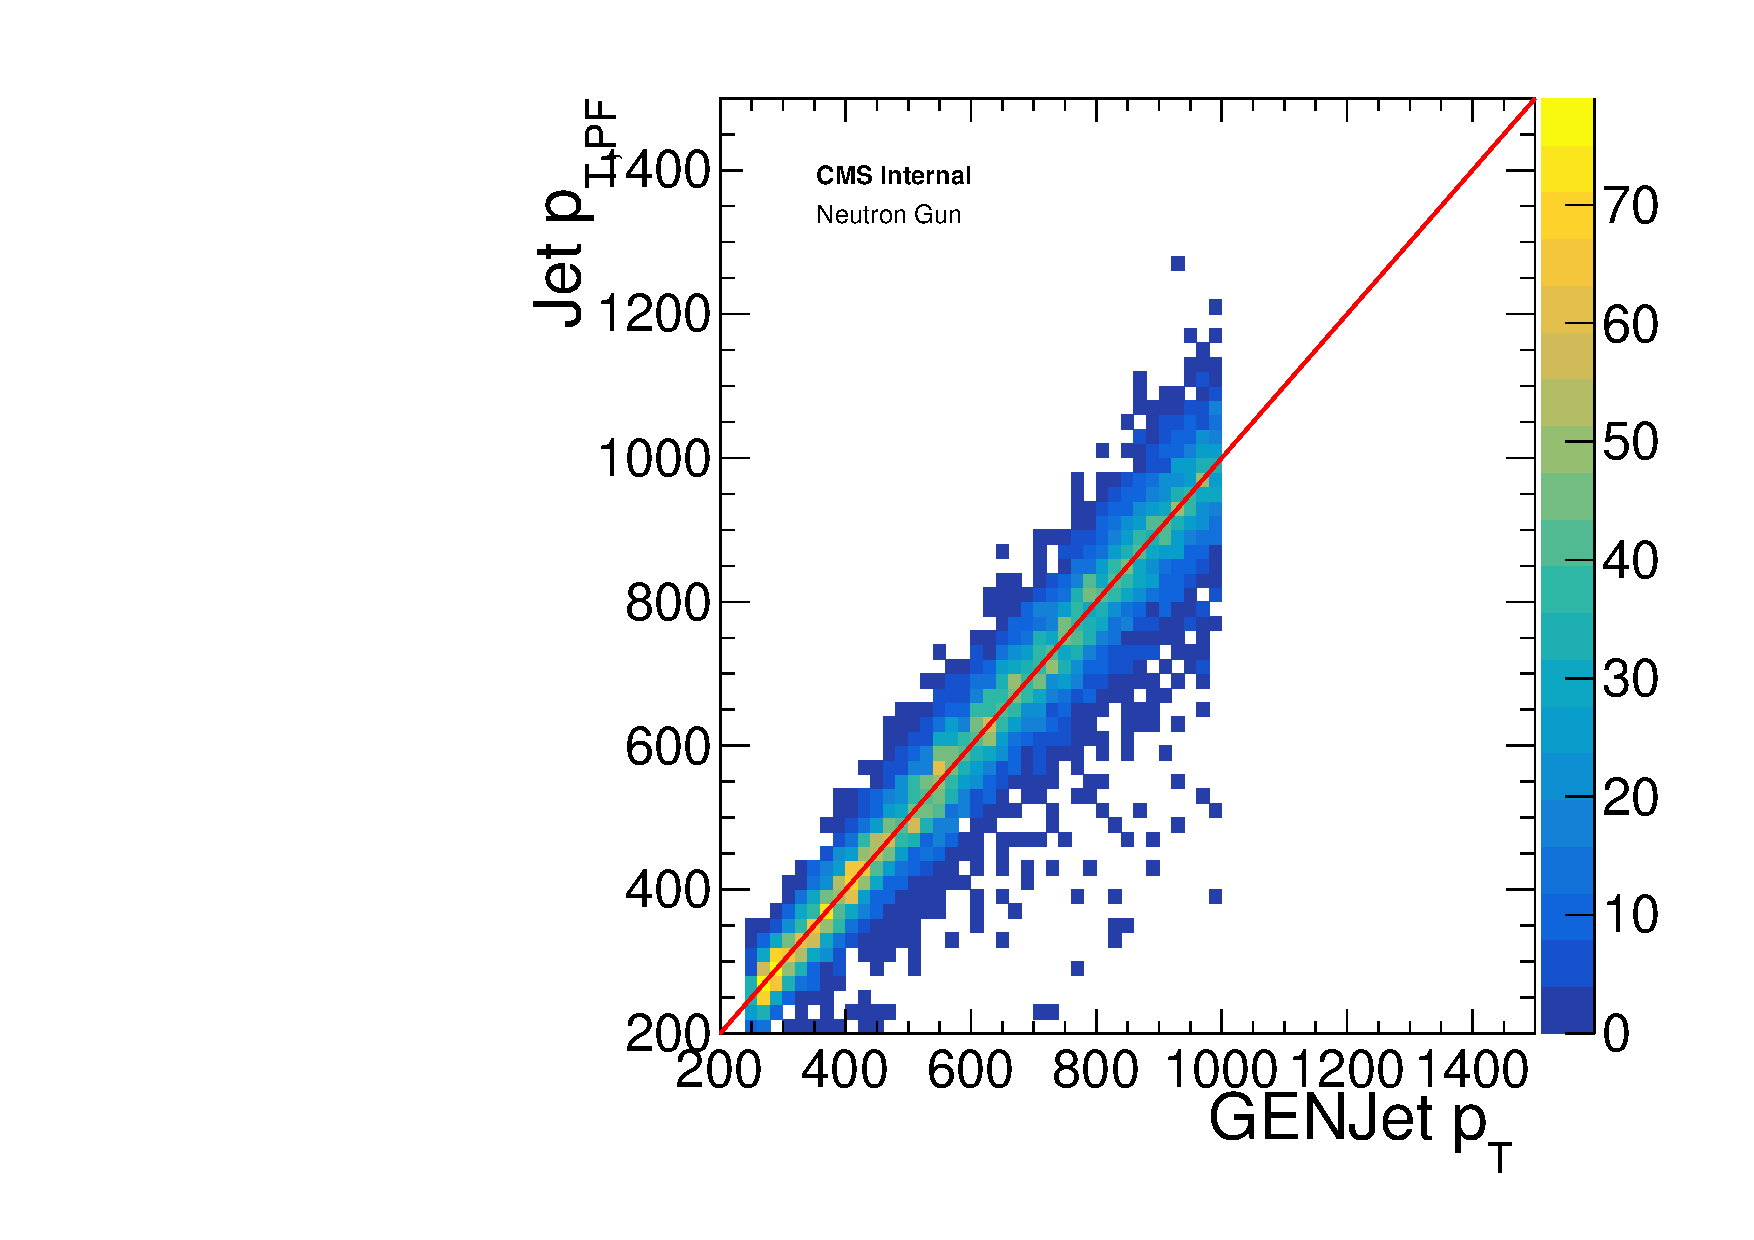
\includegraphics[width=.48\textwidth]{pt_neutron_gun_th2f_JECs_GetRandom2.pdf} \hfill
% 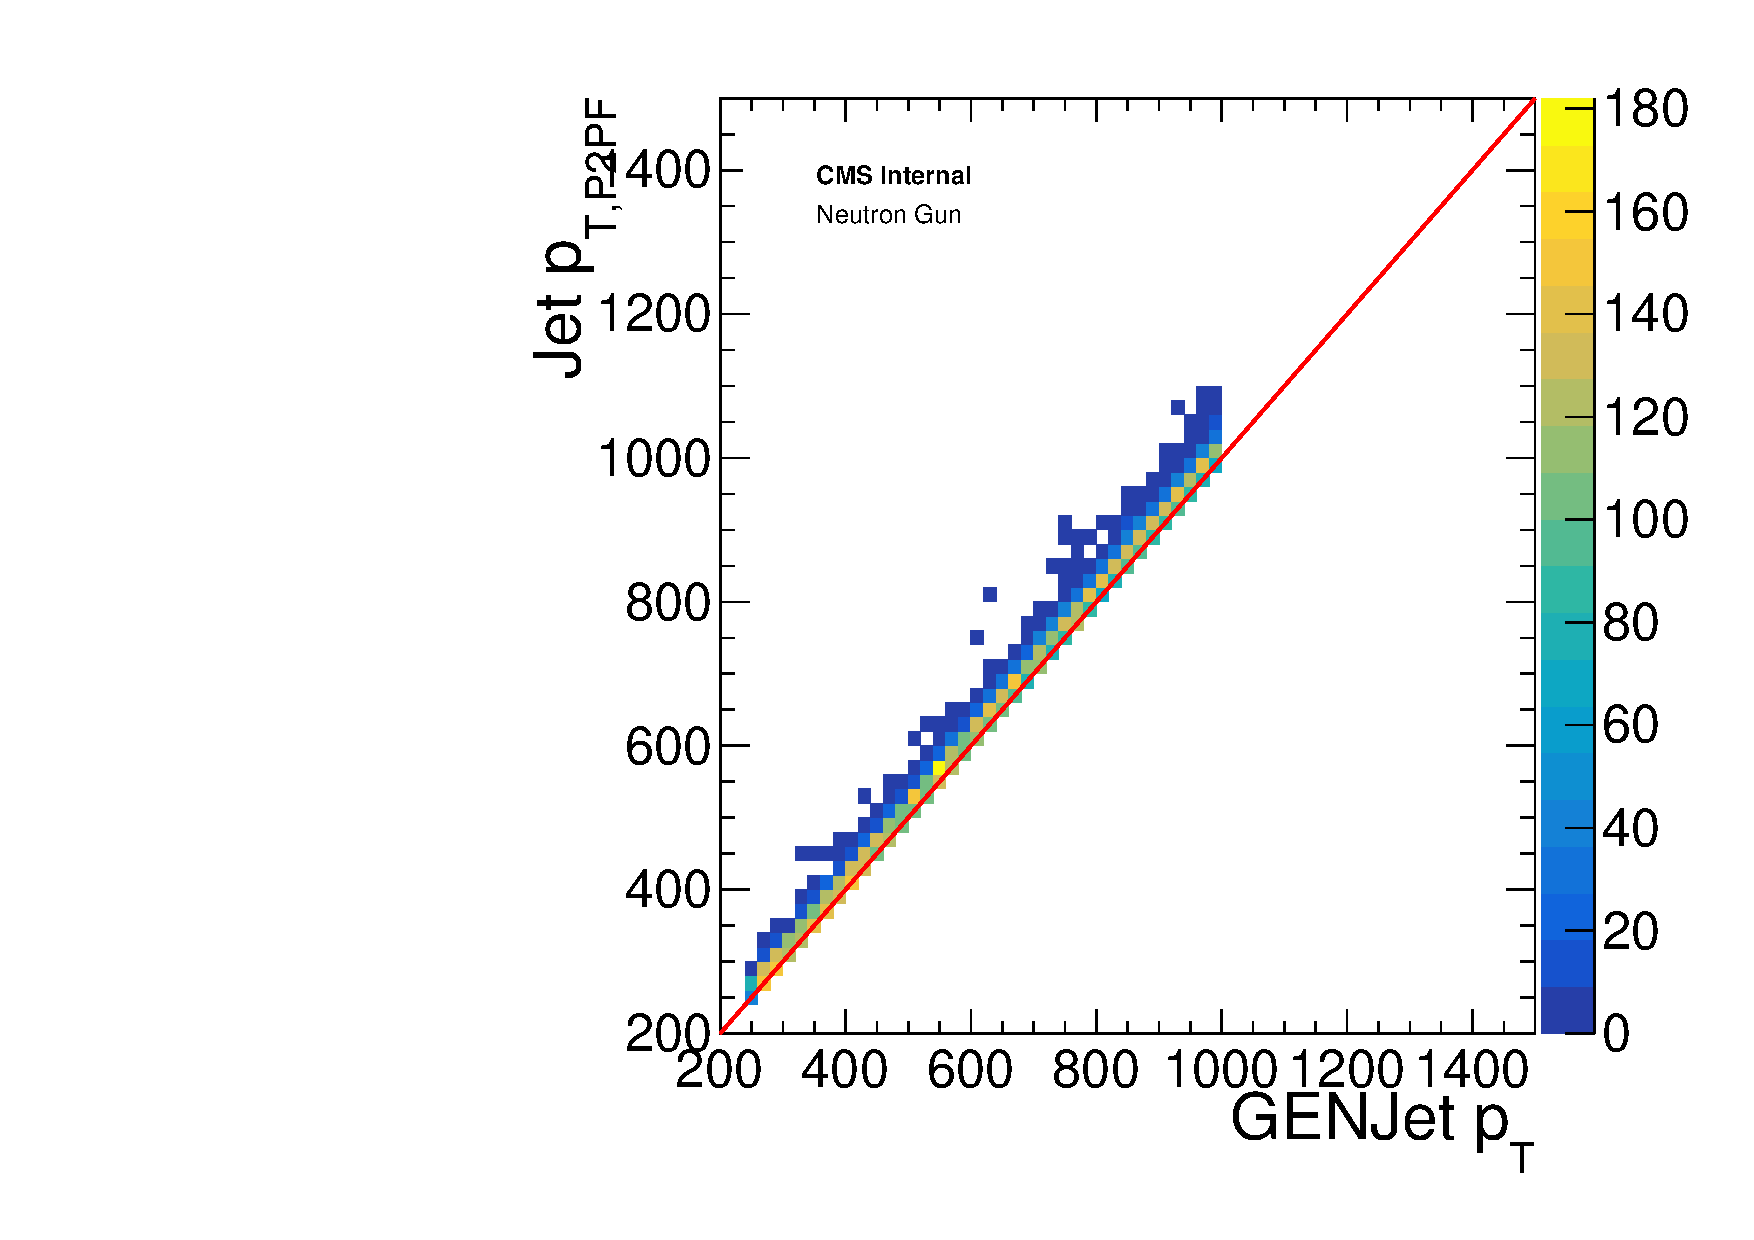
\includegraphics[width=.48\textwidth]{pt_neutron_gun_p2pf_th2f_NoSmearing.pdf}
%  \caption{Comparison of the transverse momentum of the generator-level jets to the \ac{PF} jets (left) and P2PF jets (right) without jet energy resolution smearing, using a neutron sample.}
%  \label{fig:neutron}
% \end{figure}

\begin{figure}[ht]
  \centering
 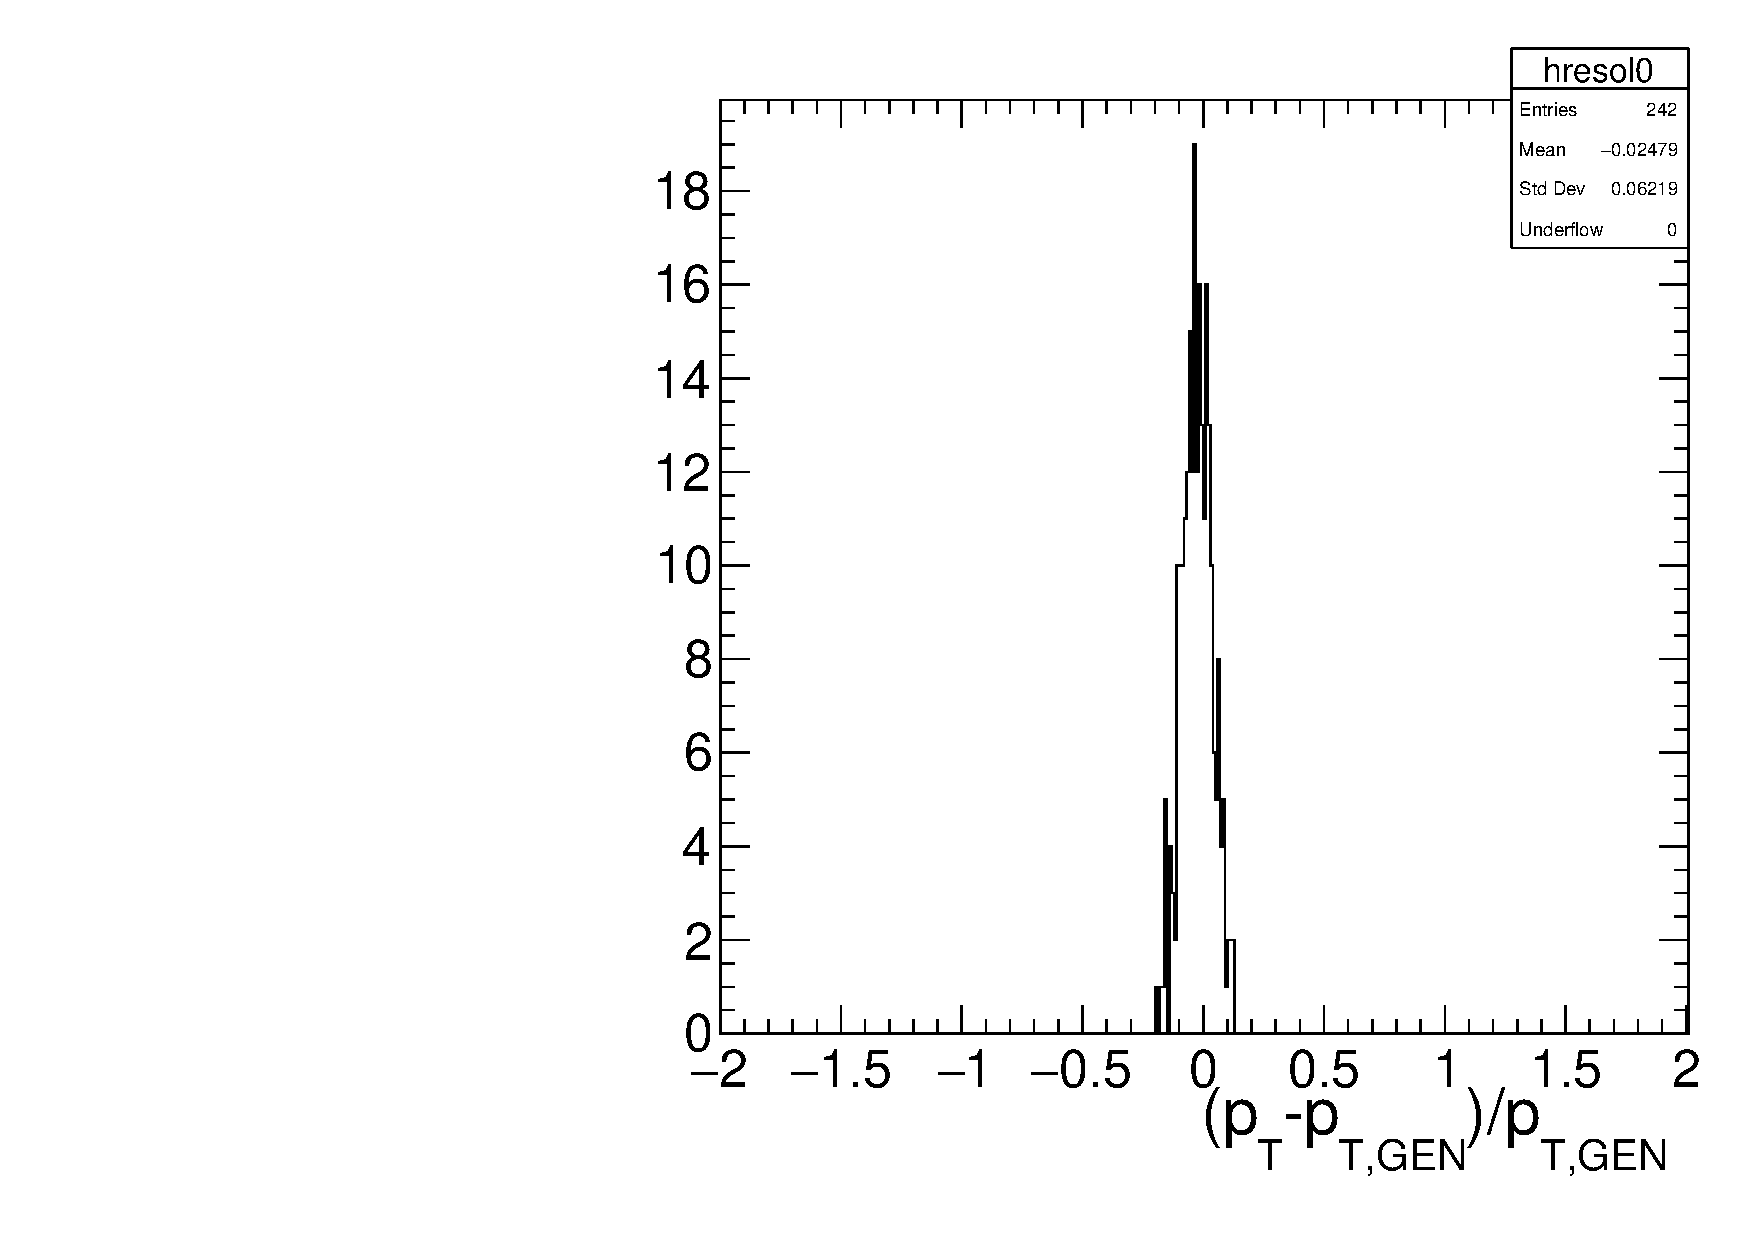
\includegraphics[width=.48\textwidth]{pt_res_ptbin_0.pdf} \hfill
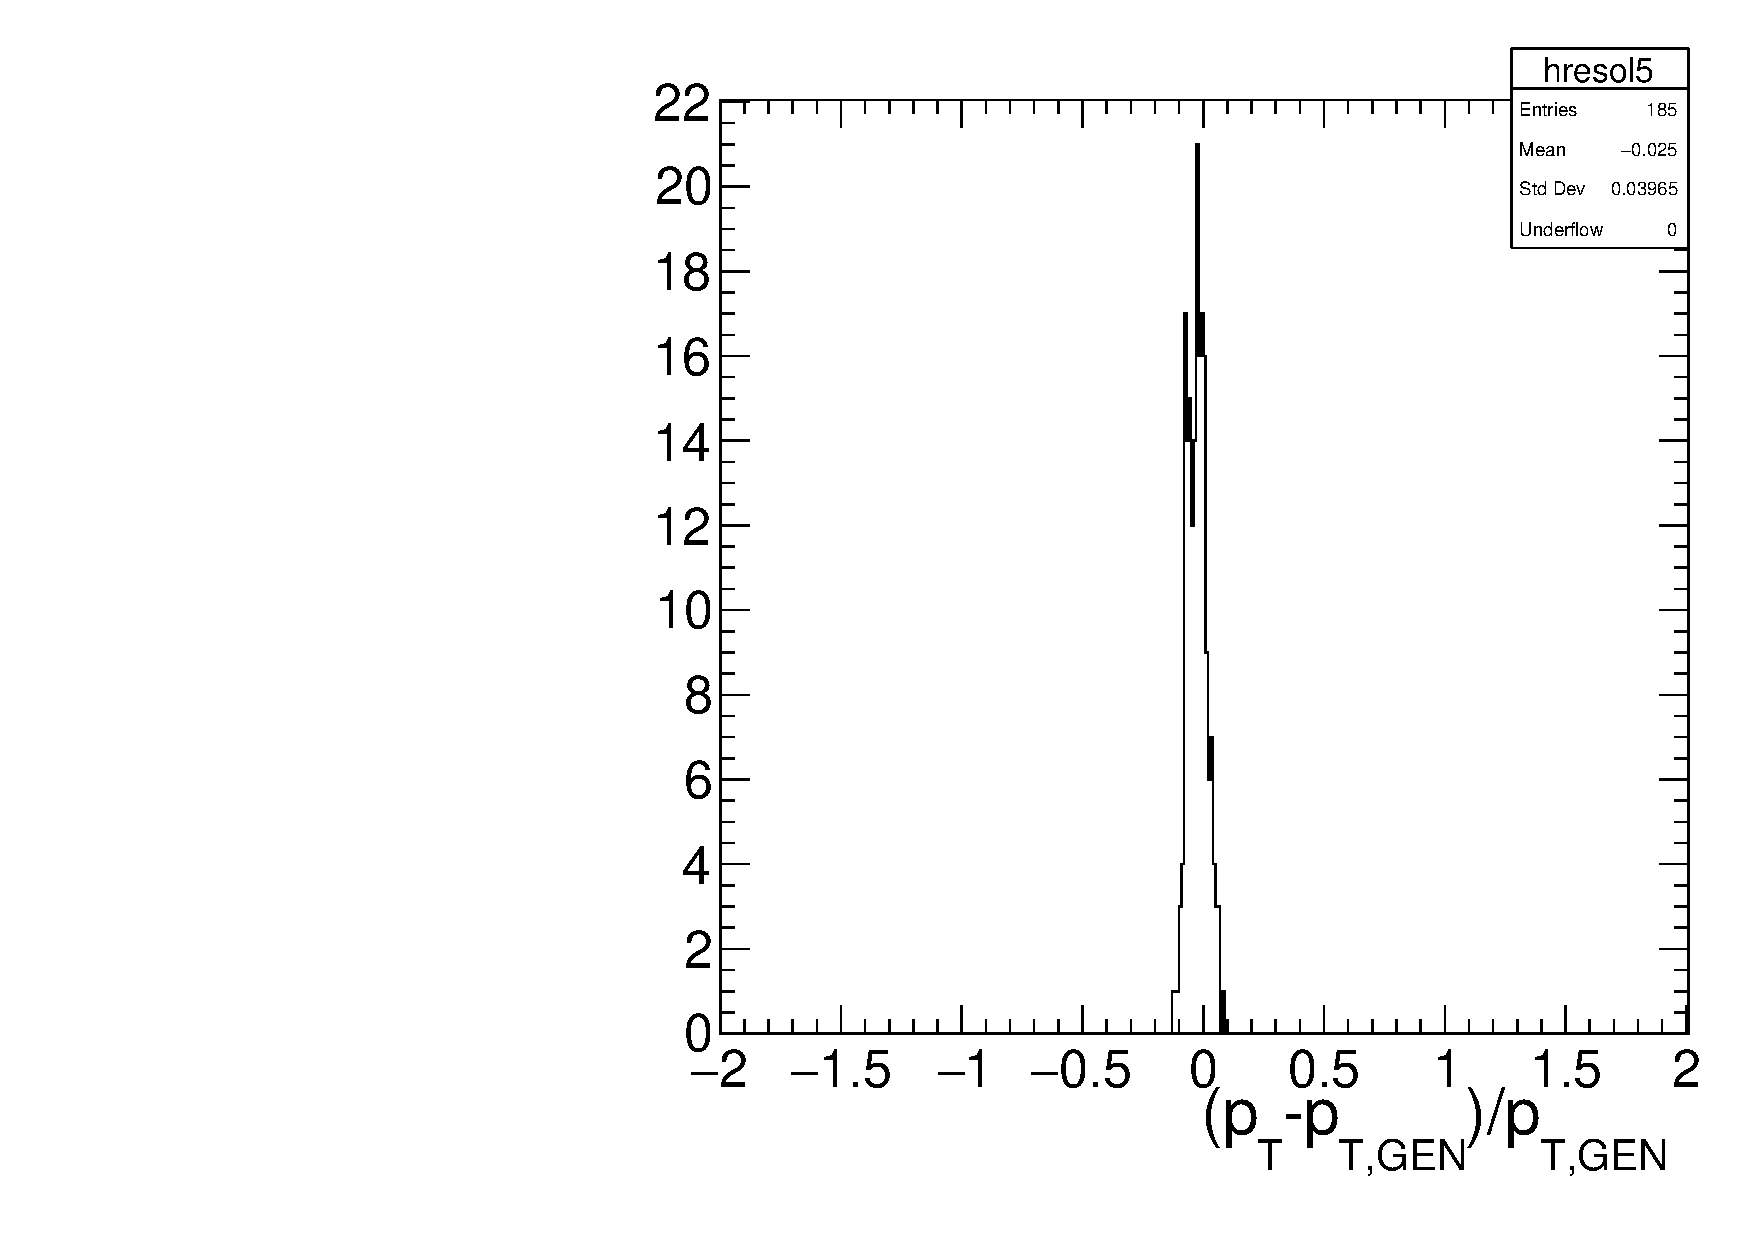
\includegraphics[width=.48\textwidth]{pt_res_ptbin_5.pdf}
 \caption{The jet energy resolution of neutrons with $0< |\eta| < 0.5$ and \SI{200}{GeV}$<p_T<$\SI{300}{GeV} (left) or \SI{700}{GeV}$<p_T<$\SI{800}{GeV} (right).}
 \label{fig:neutron_res}
\end{figure}

In order to validate this method, the custom and standard neutron samples are used to compare the two leading generator-level jets to the new jets from the custom sample, denoted as P2PF jets, and the \ac{PF} jets from the standard sample. This is illustrated in Figure~\ref{fig:neutron_corr}, where the $p_T$ of the generated neutrons is shown on the horizontal axis, and the $p_T$ of the reconstructed jet is shown on the vertical axis. The left plot shows the standard neutron sample produced with the full \textsc{Geant} simulation, while the right plot shows the custom neutron sample where the neutron was directly converted into a neutral \ac{PF} candidate. The \ac{JER} distributions are also compared in Figure~\ref{fig:neutron_res_corr} and fitted with a Crystal Ball function, showing compatible parameters.

\begin{figure}[ht]
  \centering
 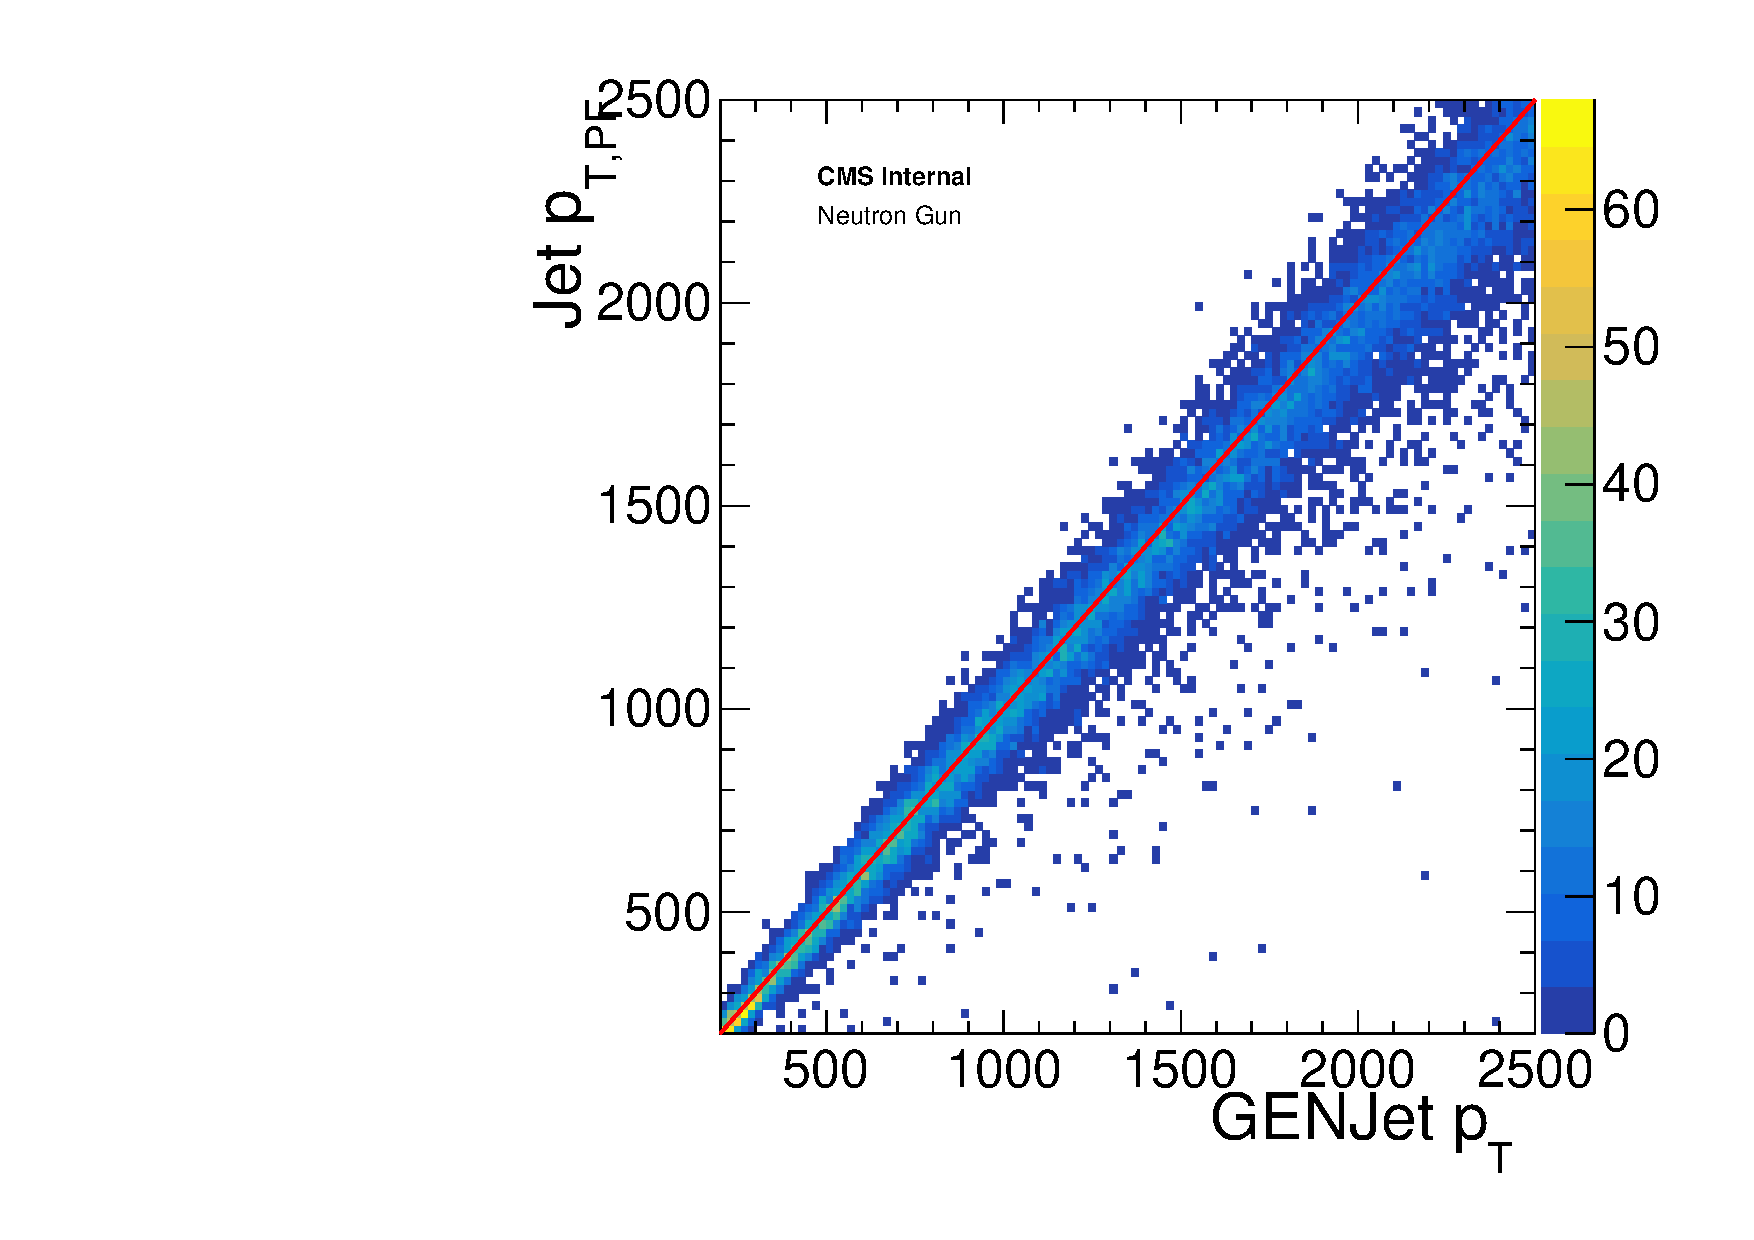
\includegraphics[width=.48\textwidth]{pt_neutron_gun_th2f_005.pdf} \hfill
\includegraphics[width=.48\textwidth]{pt_neutron_gun_p2pf_th2f_005.pdf}
 \caption{Comparison of the transverse momentum of the generator-level jets to the \ac{PF} jets (left) and P2PF jets (right) in the region $0< |\eta| < 0.5$ with jet energy resolution smearing, using a neutron sample.}
 \label{fig:neutron_corr}
\end{figure}

\begin{figure}[ht]
  \centering
 \includegraphics[width=.75\textwidth]{pt_neutron_gun_res_fit_005.pdf} 
 \caption{The jet energy resolution of the corrected P2PF jets (red) and \ac{PF} jets (black), fitted with a Crystal Ball function.}
 \label{fig:neutron_res_corr}
\end{figure}

This demonstrates that the procedure, where the \ac{JER} distributions derived from a neutron sample are used to smear the \ac{PF} candidates from generator-level \acp{SIMP}, can accurately simulate \acp{SIMP} in a realistic detector, assuming \acp{SIMP} are neutron-like. However, since this procedure directly converts the generated \acp{SIMP} into \ac{PF} candidates, the \acp{SIMP} do not interact in the Tracker and the resulting jets have a very steeply falling charged energy fraction (ChF) distribution. This gives an optimistic image, which translates in a maximal signal efficiency.

The \ac{SIMP} signal simulation and reconstruction was therefore further improved by moving to the second approach. In this method, the generated \ac{SIMP} particles are not converted into neutral \ac{PF} candidates, but they are instead replaced by neutrons, keeping the \ac{SIMP} kinematics. The standard reconstruction and full \textsc{Geant} simulation can then be applied, since the neutrons are correctly recognized and simulated. In this case, interactions will happen inside the Tracker as well and the resulting jets will contain a larger ChF, as is shown in Figure~\ref{fig:neutron_chf}. Eventually, this second method will be used in the trackless jets analysis described in Chapter~\ref{ch:SIMPs}.
 
\begin{figure}[ht]
  \centering
 \includegraphics[width=.75\textwidth]{ChF_neutrons.pdf} 
 \caption{ChF distribution of the leading jet, for a signal sample produced with the first approach (red) and the corresponding sample produced using the second method (blue).}
 \label{fig:neutron_chf}
\end{figure}

This method gives a good approximation of a \ac{SIMP} signal, since the shower generated by the \ac{SIMP} is in principle contained inside the calorimeters, as the model described in Section~\ref{sec:SIMP} is constructed so that for a specific choice of couplings the \acp{SIMP} may be detected as regular hadrons. Although the considered \ac{SIMP}-nucleon interaction is repulsive, this does not differ considerably from known attractive interactions at the probed high energies. The incoming \ac{SIMP} hits a nucleon at rest in the calorimeter, breaking it up, and because of the large incoming momentum, there is a boost forward into the calorimeter and the shower starts. The cross section would therefore be identical for a repulsive or attractive interaction and the effect on the shower is negligible since the scattering angle is very small due to the momentum boost. Furthermore, the higher the momentum of the \ac{SIMP}, the shorter the distance it travels to deposit its characteristic momentum. With the considered couplings, the depth containing a \SI{1}{GeV} \ac{SIMP} with \SI{500}{GeV} momentum is below \SI{1}{m}, within the calorimeter~\cite{Bryan}. Most of the energy will therefore be deposited in the first interaction with the material. Given the expected forward energy flow in the calorimeter shower, and the shower containment achieved by the choice of couplings in the simplified model, the shower induced by the \ac{SIMP} interaction can to first order be modelled by the interaction of a high-momentum neutral hadron, like a neutron. For the cases with a much higher \ac{SIMP} mass of \SI{700}{GeV} or \SI{1000}{GeV}, the momentum of the SIMP becomes small with respect to the \ac{SIMP} mass, which may lead to a different effect in the detector. Another difference between the interaction of neutrons and \acp{SIMP} with hadrons comes from the fact that neutrons are composite particles which will break up, while the \ac{SIMP} is a single particle. These effect are however not taken into account in the used simulation.

\clearpage
\clearpage{\pagestyle{empty}\cleardoublepage}

\graphicspath{{chapt_dutch/}{intro/}{monojet/}}

% Header
\renewcommand\evenpagerightmark{{\scshape\small Chapter 5}}
\renewcommand\oddpageleftmark{{\scshape\small The Monojet Analysis}}

\hyphenation{}

\chapter{The Monojet Analysis}
\label{ch:monojet}

As has been described in Chapter~\ref{ch:theory}, there are many searches for dark matter both at 
particle accelerators and elsewhere. At the \ac{LHC}, one very promising channel is the 
monojet search, where the detection of dark matter is done by looking for missing energy in association 
with one or more jets. The dark matter particles are expected to pass through the detector without leaving any signal since they are neutral and only interact very weakly. They can however be detected indirectly as missing energy when they recoil off one or more jets coming from initial state radiation.

First, the event selection and the estimation of the background are described, respectively in Sections~\ref{sec:selection} and \ref{sec:bkgd}. The included systematic uncertainties are described in Section~\ref{sec:syst}. In Section~\ref{sec:results}, the obtained results are shown. The improvements achieved by going from the analysis strategy used in 2015 to the 2016 version are detailed in Section~\ref{sec:improvement}. Finally, the results are interpreted in terms of the considered dark matter models in Section~\ref{sec:interpretation}.

% {\color{red}models in theory chapter?\\
% MET: add in chapter 3: + type I corrections from jets + corrections in simulation as well to match data)\\
% {\color{red} add in chapter 3: loose jet ID, pileup jet ID}.

\section{Event selection}
\label{sec:selection}

In order to select events that have the Monojet signature illustrated in Figure~\ref{fig:monojet_display}, the trigger requires either $E_T^{miss} > 90$~GeV, where $E_T^{miss}$ is the magnitude of the negative vectorial sum of the $p_T$ of all particles at trigger level, or $H_T^ {miss} > 90$ ~GeV, where $H_T^{miss}$ is calculated as the magnitude of the negative vectorial sum of the momenta of all jets with $p_T > 20$~GeV. Muons are not taken into account to compute $E_T^{miss}$ and $H_T^{miss}$, so that the same trigger can be used to select the events for the muon control regions used for the background prediction. The trigger efficiency is above 98\% for events passing the analysis selection described below.

\begin{figure}[ht]
  \centering
 \includegraphics[width=.4\textwidth]{fig.pdf} 
 \caption{Illustration of dark matter production in the monojet final state.}
 \label{fig:monojet_display}
\end{figure}

Once the events have been fully reconstructed and the jets in the event have been corrected as described in Section~\ref{sec:jet_reconstruction}, an event selection is applied by requiring the missing transverse energy $E_T^{miss}$ defined in Section~\ref{sec:MET} to be larger than 200~GeV in order to be consistent with the trigger turn-on. Additionally, the leading jet is required to have $p_T > 100$~GeV, $|\eta| < 2.5$, and to pass the loose jet identification and pileup jet identification described in Section~\ref{sec:jet_reconstruction}, as well as the jet cleaning.  The jet cleaning is done by requiring a jet charged hadron energy fraction CHF $> 0.1$ and a jet neutral hadron energy fraction NHF $< 0.8$. The same requirements are applied for the remaining jets to be taken into account, except for the $p_T$ threshold which is at 30~GeV in this case. A cut on the difference in azimuthal angle between the $E_T^{miss}$ and the first four leading jets of $\Delta\phi(jet, E_T^{miss}) > 0.5$ is also applied to suppress the QCD background from mismeasurements of jet momentum or detector noise. The events are further cleaned by applying quality filters to remove events with badly reconstructed missing transverse energy. Finally, events containing a lepton, a photon, or a b-jet are vetoed as well.

The leptons are vetoed to suppress the electroweak backgrounds, such as $W(lv)$ + jets and semileptonic diboson decays. Electrons (muons) are considered for the veto if they pass the loose selection, described in Section~\ref{sec:electron_ID}~(\ref{sec:muonID}), and have $p_T > 10$~GeV and $|\eta| < 2.5 (2.4)$. In the case of tau leptons, they are required to have $p_T > 15$~GeV and $|\eta| < 2.3$. They should also pass the tau identification criteria, which require a jet with an identified subset of particles with a mass consistent with the decay products of a hadronic tau and which are isolated with a pileup corrected isolation cut requiring less than 5~GeV of energy deposits within a radial cone of $\Delta R < 0.3$. Photons are required to have $p_T > 15$~GeV, $|\eta| < 2.5$, and to pass the loose identification criteria described in Section~\ref{sec:electron_ID}. The photon veto is added to suppress the $Z(\nu\nu)$ + photon + jets and $W(l\nu)$ + photon + jets background processes, and to ensure there is no overlap with a similar dark matter search which investigates the final state consisting of missing energy and a photon. This rejects less than 1\% of the signal. Finally, the b-jet veto reduces the top background by a factor 3 and only reduces the signal by 5 to 10\%, depending on the type and mass of the mediator. The b-jets are tagged with the Combined Secondary Vertex algorithm described in Section~\ref{sec:btagging}, using the loose working point.

\section{Background estimation}
\label{sec:bkgd}

% {\color{red} muons: muon veto to suppress electroweak bkgds
% pt > 10, eta < 2.4, loose selection:
% muons for control regions: global, pf, global track chi2 < 10, global track fit includes >= 1 muon chamber hit, muon segments in >= 2 muon stations, transverse impact parameter wrt PV < 2mm, longitudinal impact parameter < 5mm, >= 1 pix hit, > 8 trk layers hit, hits in >= 5 tracker layers, delta beta < 0.12
% 
% electrons: electron veto to suppress electroweak bkgds
% pt > 10, eta < 2.5,  loose selection(table 10)
% electrons in control region: tight selection (table 11)
% 
% photons in control region to estimate Znunu bkgd: tighter selection table 13
% < 1\% rejection of signal
% For muons and
% electrons this reduces the influence of large brehmstrahlung, further minimizing anomalous
% effects that would modify the recoil.
% 
% photon purity (2 methods):
% 
% lepton and photon eff: 2 methods}

The dominant background comes from $Z$ + jet events where the $Z$ boson decays to two neutrinos. This produces the same signature of jets with missing energy as the signal, and results in an irreducible background. The second largest background consists of $W$ + jets events with a leptonically decaying $W$ boson. This background is already suppressed by the lepton veto, but a fraction of these events remain when the lepton is either not identified or outside of the detector acceptance. The remaining background events come from top quark decays, which are suppressed by the b-jet veto, semileptonic diboson ($WW$, $WZ$, and $ZZ$) decays, and QCD multijet events. The two main background contributions are estimated from five control regions in data consisting of dimuon, dielectron, single muon, single electron, and photon + jets events. The $E_T^{miss}$ in these control regions is redefined in order to imitate the $E_T^{miss}$ shape in the signal region. This hadronic recoil $U$ is obtained by removing the leptons or the photon from the $E_T^{miss}$ computation. The contributions from top quark decays and semileptonic diboson decays are estimated using simulated samples, while the QCD multijet background is estimated using a data-driven approach.

\subsection{The \boldmath$Z$ and \boldmath$W$ background estimation}

The yield of $Z(\nu\nu)$ and $W(l\nu)$ + jets events in the signal region is estimated from five control regions by using the ratio between data and MC in the control region, per bin of the recoil distribution. For the prediction using $Z\rightarrow \mu\mu$ events in the dimuon control region for example, the predicted yield of $Z\rightarrow\nu\nu$ events is given by
\begin{align}
 N_{Z(\nu\nu)} &= \frac{N_{Z(\mu\mu)}^{data}}{N_{Z(\mu\mu)}^{MC}}\ N_{Z(\nu\nu)}^{MC}\\
 &= \frac{N_{\mu\mu}^{data} - N_{Bkgd}}{N_{Z(\mu\mu)}^{MC}}\ N_{Z(\nu\nu)}^{MC} \\
 &= \frac{N_{\mu\mu}^{data} - N_{Bkgd}}{N_{Z(\mu\mu)}^{MC}}\ R_{Z(\mu\mu)\rightarrow Z(\nu\nu)}\ N_{Z(\mu\mu)}^{MC}
\end{align}
The transfer factors, denoted by $R$, are derived from simulation and take into account the impact of lepton acceptance and efficiency, as well as the additional $E_T^{miss}$ requirement for the single electron control region. They also include the difference in branching ratio and the relation between the differential cross sections of the photon, $W$, and $Z$ boson production as a function of the boson $p_T$. The transfer factors are computed as a function of the recoil, and are shown for the five different control regions in Figure~\ref{fig:TF}. Furthermore, the $Z/W$ ratio shown in the bottom right plot of Figure~\ref{fig:TF} provides an additional constraint since the single lepton control regions are also used to  estimate the $Z(\nu\nu)$ + jets background.

\begin{figure}[ht]
  \centering
 \vspace{.3cm}
 \includegraphics[width=.49\textwidth]{dimuon_TF.png} 
 \includegraphics[width=.5\textwidth]{single_muon_TF.png} \\
 \vspace{.4cm}
 \includegraphics[width=.49\textwidth]{dielectron_TF.png} 
 \includegraphics[width=.5\textwidth]{single_electron_TF.png} \\
 \vspace{.2cm}
 \includegraphics[width=.49\textwidth]{gamma_TF.png} 
 \includegraphics[width=.5\textwidth]{ZW_ratio.png} 
 \caption{Transfer factors for the dimuon (top left), single muon (top right), dielectron (middle left), single electron (middle right), and photon + jets (bottom left) control regions. The ratio of the $Z$ and $W$ transfer factors is shown in the bottom right plot.}
 \label{fig:TF}
\end{figure}

The simulated samples used for the background estimation are generated at leading order (LO) using the \textsc{Madgraph} generator, and corrected to next-to-leading order (NLO). These corrections introduce an additional systematic uncertainty, but are crucial in order correctly represent the data, since the simulation is approximately 40\% higher than the data when using only LO calculations. The NLO QCD k-factors are derived from samples generated at NLO with \textsc{MadGraph5\_}a\textsc{MC@NLO}, while the electroweak k-factors are obtained from theoretical calculations~\cite{Kuhn:2005gv, Kallweit:2015fta, Kallweit:2014xda, Kallweit:2015dum}. The differential cross section as a function of the boson $p_T$ is shown in Figure~\ref{fig:kfactors} for photon, $W$,and $Z$ production, and the obtained k-factors are displayed in the ratio plots. More details on the different control regions are given in the following description.

\begin{figure}[ht]
  \centering
 \includegraphics[width=.49\textwidth]{Z_EWK_kfactor.pdf} 
 \includegraphics[width=.49\textwidth]{W_EWK_kfactor.pdf} \\
 \includegraphics[width=.49\textwidth]{gamma_EWK_kfactor.pdf} 
 \caption{ The differential cross section as a function of the boson $p_T$ for photon, $W$,and $Z$ production, with the resulting k-factors in the ratio plots.}
 \label{fig:kfactors}
\end{figure}

\begin{itemize}
 \item[] \textbf{Dimuon control region}\\ The traditional control region for the $Z$ boson background is the dimuon control region. This region is dominated by $Z\rightarrow\mu\mu$ events, which are very similar to the $Z(\nu\nu)$ + jets background events, the only difference being the decay mode. The production mode and kinematics in the control region are very similar, as well as the acceptance. However, the branching ratio of the $Z$ boson into two muons is 6 times smaller than the branching ratio to two neutrinos. As a result, the dimuon control region contains about 10 times less $Z$ boson events than the signal region. In order to improve this statistical limitation, other control regions have been added as well.

In the dimuon control region the events are selected using the monojet triggers and applying the same requirements as described in Section~\ref{sec:selection} for the signal region, using the recoil instead of the missing transverse energy, except for the muon veto. Additionally, exactly two muons with opposite charge and with $p_T > 10$~GeV should be identified using the loose identification described in Section~\ref{sec:muonID}. At least one muon is required to have $p_T > 20$~GeV and to pass the tight selection requirements described in Section~\ref{sec:muonID}, and the leading muon should also have a transverse momentum large than 20~GeV. Finally, the dimuon mass should be between 60 and 120~GeV, corresponding to the $Z$ boson mass.

\item[] \textbf{Single muon control region}\\ In order to model the second largest background, coming from $W(l\nu)$ + jets events, a single muon control region is typically used. This control region is in addition also used to constrain the $Z(\nu\nu)$ + jets background. The events in the single muon control region are required to pass the monojet triggers and event selection replacing the $E_T^{miss}$ by the recoil obtained by removing the muon, except for the muon veto. One muon should then pass the tight selection requirements and have $p_T > 20$~GeV.

\item[] \textbf{Dielectron and single electron control region}\\ The dielectron and single electron control regions are completely analogous to the dimuon and single muon control regions, respectively. These events are required to pass the single electron triggers. Similarly to the dimuon control region, the events in the dielectron control region are required to pass the monojet selection, except for the electron veto. Instead, exactly two electrons with $p_T > 10$~GeV are required to pass the loose identification described in Section~\ref{sec:electron_ID}. In addition, at least one electron should pass the tight selection requirements and have $p_T > 20$~GeV. Finally, the dielectron mass should be between 60 and 120~GeV, in order to be consistent with a $W$ boson decay. {\color{red}transfer factor last bin due to isolation in trigger}. The dielectron control region is used to constrain the $Z\rightarrow\nu\nu$ background while the single electron control region is used to constrain the $W(l\nu)$ + jets background. In the single electron control region, the events are required to have one electron passing the tight selection requirements and having $p_T > 20$~GeV, analogously to the single muon control region. In this region, a large amount of QCD background is present. In order to reject most of those events, an additional cut on the $E_T^{miss}$, which includes the single electron, is added at 50~GeV. This reduces the QCD background by an order of magnitude.

\item[] \textbf{Photon + jets control region}\\Due to its large yield, photon + jets control region provides the dominant constraint on the high-$p_T$ part of the $Z(\nu\nu)$ + jets background. The selection of these events is done using the single photon triggers and applying the monojet selection, except for the photon veto. One photon is then required to pass the tight identification described in Section~\ref{sec:electron_ID} and to have $p_T > 175$~GeV and $|\eta| < 1.4442$. Events with more than one photon passing the loose identification requirements described in Section~\ref{sec:electron_ID} are rejected.
\end{itemize}

\subsection{The QCD background estimation}

\section{Systematic uncertainties}
\label{sec:syst}

For the main backgrounds, multiple systematic uncertainties on the transfer factors are taken into account. Experimental uncertainties are added for the muon efficiency, the electron efficiency, the lepton veto, the photon efficiency, and the photon purity in the photon + jets sample. 

Uncertainties are also added from theory, to take into account variations of the factorization and renormalization scales, PDF uncertainties, and the NLO electroweak corrections. The former 3 uncertainties are shown in Figure~\ref{fig:kfactors_unc} for the $Z$ + jets, $W$ + jets, and photon + jets samples. The  uncertainties are then propagated to the transfer factors, and are displayed in Figure~\ref{fig:transfer_factors_unc}. To evaluate the PDF uncertainty, the samples are reweighted with event-by-event scale factors representing the shift in the kinematic distributions from variations in the PDF. The transfer factors are then produced for each variation, and the RMS of the variation is taken as PDF uncertainty. Similarly, the renormalization and factorization scales are varied up and down by a factor 2, and the uncertainties are derived from the resulting transfer factors. For the electroweak corrections, the full correction is taken as an uncertainty.

\begin{figure}[ht]
  \centering
 \includegraphics[width=.49\textwidth]{Z_uncertainties_smooth.pdf} 
 \includegraphics[width=.49\textwidth]{W_uncertainties_smooth_new.pdf} \\
 \includegraphics[width=.49\textwidth]{gamma_uncertainties_smooth.pdf} 
 \caption{The PDF, renormalization, and factorization scale uncertainties for the $Z$ + jets (top left), $W$ + jets (top right), and photon + jets (bottom) samples. The uncertainties from the renormalization and factorization scales are obtained by separately varying them up and down by a factor 2.}
 \label{fig:kfactors_unc}
\end{figure}

\begin{figure}[ht]
  \centering
 \includegraphics[width=.49\textwidth]{fig.pdf} 
 \includegraphics[width=.49\textwidth]{fig.pdf}
 \caption{.}
 \label{fig:transfer_factors_unc}
\end{figure}

\section{Results}
\label{sec:results}

The results are extracted by performing a binned fit to the missing energy spectrum, fitting simultaneously over the five control regions and the signal region. 

\section{Improvement going from the 2015 to 2016 analysis}
\label{sec:improvement}

One of the improvements that were added to the monojet analysis is the use of MC samples generated at leading order for the estimation of the main backgrounds. This was possible by generating samples that are binned in photon, $Z$, or $W$ boson $p_T$. As a result, no k-factors need to be applied to samples generated at LO and no additional systematic uncertainties need to be introduced for this.

\section{Interpretation}
\label{sec:interpretation}

\clearpage{\pagestyle{empty}\cleardoublepage}

\graphicspath{{chapt_dutch/}{intro/}{simps/}}

% Header
\renewcommand\evenpagerightmark{{\scshape\small Chapter 5}}
\renewcommand\oddpageleftmark{{\scshape\small Search for SIMPs using Trackless Jets}}

\renewcommand{\bibname}{References}

\hyphenation{}

% STILL NEED TO CHECK ORDER OF DETAILS, OFTEN ONLY COME AFTER STATEMENT, E.G. PT DEPENDENCE OF CHF DUE TO RECO AND 1- AND 2-LEG PREDICTION.

\chapter{Search for SIMPs using Trackless Jets}
\label{ch:SIMPs}

The monojet dark matter search detailed in Chapter~\ref{ch:monojet} can be complemented at high interaction cross sections by a different search which does not look for dark matter in the form of missing transverse momentum. Indeed, if the dark matter particles have an interaction cross section of the order of the strong interaction, they will interact in the detector, mainly in the calorimeters. The analysis described in this chapter is based on this scenario, and the considered simplified model is specified in Section~\ref{sec:SIMP_model}. In this model, the dark matter particles are produced in pairs through a new strongly interacting mediator, and give rise to a pair of trackless jets as signature. Since the produced \acfp{SIMP} are neutral, the resulting jets can be distinguished from \acs{QCD} jets using the jet charged hadron energy fraction (CHF). The signal region where the \acp{SIMP} are being looked for is therefore defined by requiring the two leading jets to have a low CHF. In the control region, which is used to predict and validate the expected background, one or both jets are required to have a large CHF.

Firstly, the applied jet and photon reconstruction and identification are described, as well as the specific treatment applied for the primary vertex selection. The triggers that were designed specifically for this search, exploiting the CHF, are outlined in Section~\ref{sec:SIMP_trigger}. However, these triggers were found to be problematic and eventually a generic single jet trigger was used instead. Next, the event selection is detailed in Section~\ref{sec:SIMP_selection} for both the signal and control regions. The strategy for the background estimation and the systematic uncertainties are discussed in Sections~\ref{sec:SIMP_backgrounds} and \ref{sec:SIMP_systematics}, respectively. Finally,  in Sections~\ref{sec:SIMP_results} and \ref{sec:SIMP_interpretation}, the results are shown and interpreted in terms of the \ac{SIMP} simplified model described in Section~\ref{sec:SIMP}.

\section{Physics object reconstruction} 
\label{sec:SIMP_reconstruction}

In this analysis, jets with a very small charged hadron energy fraction (CHF) are being searched for. Since these are rather peculiar jets containing no or very few tracks, a good primary vertex selection and photon identification play an important role in suppressing the main physics and reconstruction backgrounds.

\subsection{Jets}

For the jet reconstruction, the standard method described in Section~\ref{sec:jet_reconstruction} is used. Although the jets in the signal samples are expected to be neutral, it is beneficial to use \ac{PF} jets because they directly provide an unambiguous association of tracks to jets. The standard jet energy corrections are applied as well, while the standard jet identification criteria are not used, since several of the quality criteria would actually remove the neutral \ac{SIMP} jets.

\subsection{Photons}

Since photons might be reconstructed as neutral jets, photon + jets events are an important background for the control as well as the signal region. The photons therefore need to be identified and rejected, which is done using the standard photon loose identification described in Section~\ref{sec:electron_ID}. Further photon rejection is achieved by analysis-specific selections on photon conversions and on the jet neutral electromagnetic energy fraction (NEMF), as described in Section~\ref{sec:SIMP_selection}.

\subsection{Primary vertex}

% In the standard primary vertex reconstruction, the vertex with the highest $\sum p_T^2$ is chosen, where the sum runs over the tracks associated to the vertex following the application of a deterministic annealing filter which assigns weights to sufficiently high-quality tracks that enter the vertex fit~\cite{Chatrchyan:2014fea}. While in events with jets many tens of high-momentum tracks can usually be associated to a primary vertex, thus making primary vertex finding almost fully efficient and pure, in the case of a pair of neutral jets this is not the case any more. The underlying event and potentially initial state \acs{QCD} radiation can still provide some tracks, but in extreme cases a wrong vertex is chosen, arising from a hard pileup collision.

The standard primary  vertex reconstruction described in Section~\ref{sec:tracking} sometimes provides a wrong primary vertex, which arises from a pileup interaction. The choice of a wrong vertex is not a problem in the case of signal events, which will pass in particular the CHF cuts in the event selection detailed in Section~\ref{sec:SIMP_selection} just as easily. However, a wrongly chosen vertex in a \acs{QCD} background event leads to the jets having an artificially very low CHF, both in simulation and data, as the standard \acf{CHS} procedure will remove the tracks from the vertex of the true hard interaction. This makes such events appear signal-like. For the lowest jet charged hadron energy fractions considered in this analysis, this background of events with a misidentified primary vertex becomes dominant with respect to the background from \acs{QCD} events with a very rare jet fragmentation into predominantly neutral hadrons and photons. In Figure~\ref{fig:wrongvertex} an event display is shown that demonstrates such a wrong choice of vertex.

\begin{figure}[ht]
  \centering
  \includegraphics[width=0.99\textwidth]{figures/wrongvertex.png}
  \caption{Event display showing an example of a wrong primary vertex selection in a MC simulated QCD event. Although "Vertex 2" is the real vertex of the hard collision, "Vertex 1" is selected because of the presence of a single high-$p_T$ track with poor momentum resolution and no pixel hits attached. As a result, the two visible high-$p_T$ jets (above \SI{200}{GeV}), clearly with many tracks attached, are reconstructed with only 3\% and 4\% of charged energy fraction.}
  \label{fig:wrongvertex}
\end{figure} 

Investigating this problem, many events with a wrong vertex assignment were observed to have the highest-$p_T$ track being of poor quality, with a high momentum with large uncertainty, and no pixel hits. This alone, though, does not provide a sufficient handle to suppress this background, and a plain cut on number of pixel hits was verified to remove a lot of signal events as well.
% plot or numbers to show reduction in signal?
Studying the simulated \ac{QCD} multijet events with a very low CHF coming from primary vertex misidentification by analysing event displays also showed that the true vertex is reconstructed as the second vertex in the list for the far majority of the cases. A second jet reconstruction was therefore produced, based on selecting the second entry in the list of primary vertices to be the event's collision vertex, and rerunning the \ac{CHS} as well. If this second vertex was the correct one, the jets will now have a large CHF in most of the cases, while the first event reconstruction yields low-CHF jets. In the event selection discussed in Section~\ref{sec:SIMP_selection}, it is then sufficient to ask both event reconstructions to pass the cut of low jet CHF, effectively suppressing this background induced from wrong primary vertex selection.

\section{Trigger selection}
\label{sec:SIMP_trigger}

Several triggers have been designed specifically for this analysis, as shown in Table~\ref{tab:triggers}. Four triggers were available to select signal events, denoted as ``signal'' in the table and providing a trade-off between a high CHF and a low jet $p_T$. The CHF cut is always applied on both jets. Two additional triggers, indicated with the ``control'' type, were used to determine the trigger efficiencies. These triggers were prescaled, meaning that only a fraction of the events are kept due to the otherwise very high rate of the trigger.

\begin{table}[ht]
  \centering
  \begin{tabular}{| l | c | c |}
    \hline
    Trigger name & Type & Int. Lumi. \\
    \hline
    \verb|HLT_DiCentralPFJet170_CFMax0p1_v*|     & Signal  & $33.1 \, \mathrm{fb}^{-1}$ \\
    \verb|HLT_DiCentralPFJet220_CFMax0p3_v*| \tablefootnote{Due to the unexpected high rate, this trigger was disabled after some time.}    & Signal  & $5.91 \, \mathrm{fb}^{-1}$ \\
    \verb|HLT_DiCentralPFJet330_CFMax0p5_v*|     & Signal  & $33.1 \, \mathrm{fb}^{-1}$ \\
    \verb|HLT_DiCentralPFJet430_v*|              & Signal  & $33.1 \, \mathrm{fb}^{-1}$ \\
    \verb|HLT_DiCentralPFJet170_v*|              & Control & $0.101 \, \mathrm{fb}^{-1}$ \\
    \verb|HLT_SingleCentralPFJet170_CFMax0p1_v*| & Control & $0.375 \, \mathrm{fb}^{-1}$ \\
    \hline
  \end{tabular}
  \caption{Summary of the triggers designed for this analysis.}
  \label{tab:triggers}
\end{table}

These triggers were designed by using \acs{QCD} samples to test their performance before using them in data taking, since the signal samples do not simulate the trigger behaviour. The trigger efficiency of \texttt{HLT\_DiCentralPFJet330\_CFMax0p5} as a function of $p_{T}$ and CHF is shown in Figure~\ref{fig:efficiencies_qcd_data}, using data and simulated \acs{QCD} events. The signal efficiency measurement was first tried by taking a photon + jet sample, as photons could also mimic neutral jets. The photon was matched to the leading jet and the efficiency was measured at low CHF. However, the photon is in many cases reconstructed as an electron by the \ac{PF} algorithm. Thus, the jet is reconstructed with a large electromagnetic energy fraction (EMF) and it does not mimic the \ac{SIMP} signal. 

\begin{figure}[ht]
  \centering
  \includegraphics[width=0.47\textwidth]{figures/trigger/pt_eff_05_DataMC.png}\hfill%
  \includegraphics[width=0.47\textwidth]{figures/trigger/chf_eff_05_DataMC.png}
  \caption{The \texttt{HLT\_DiCentralPFJet330\_CFMax0p5} trigger efficiency as a function of $p_{T}$ (left) and CHF (right). Comparison between data (black) and \acs{QCD} simulation (red). }
  \label{fig:efficiencies_qcd_data}
\end{figure}

Instead, one of the neutron signal samples described in Section~\ref{sec:SIMPs} was used, generated with a \ac{SIMP} mass of \SI{700}{GeV}. The obtained trigger efficiency as a function of $p_{T}$ and CHF is shown in Figure~\ref{fig:efficiencies_simp_data} for \texttt{HLT\_DiCentralPFJet330\_CFMax0p5}, comparing the data and the signal-like events. This shows that the trigger reaches a plateau at only 60\% signal efficiency. The origin of the inefficiency was found to come from a requirement asking at least one charged particle in the jets. This explains why the trigger efficiencies turn on at the expected values when using data or simulated \acs{QCD} events, while it is largely inefficient in signal-like simulation which generates neutral jets.

\begin{figure}[ht]
  \centering
  \includegraphics[width=0.47\textwidth]{figures/trigger/pt_eff_05_DataSIMP.png}\hfill%
  \includegraphics[width=0.47\textwidth]{figures/trigger/chf_eff_05_DataSIMP.png}
  \caption{The \texttt{HLT\_DiCentralPFJet330\_CFMax0p5} trigger efficiency as a function of $p_{T}$ (left) and CHF (right). Comparison between data (black) and signal-like MC (red).}
  \label{fig:efficiencies_simp_data}
\end{figure}

Consequently, the single jet trigger \texttt{HLT\_PFJet450} has been used for the analysis. It was selected because it has the lowest threshold among the unprescaled\footnote{Triggers with a lower $p_T$ threshold exist, but these are prescaled. Prescaled triggers are typically not used to perform an analysis, as only a small fraction of the events that pass the trigger are kept, leading to large statistical uncertainties.} single jet triggers. The trigger efficiency for the data was measured using the single muon events, and is defined as
\begin{equation}
\epsilon = \frac{\mathrm{Obs}(\texttt{HLT\_PFJet450}\ \mathrm{and}\ \texttt{HLT\_IsoMu24})}{\mathrm{Obs}(\texttt{HLT\_IsoMu24})},
\end{equation} 
where Obs in this case is the $p_T$ spectrum of the leading jet for events that fired the single muon (and single jet) trigger. The jets are required to have a muon energy fraction smaller than $0.3$ in order to avoid jets with large difference in the online and offline $p_T$. This difference can arise when the offline \ac{PF} jet contains a high-$p_T$ muon. Since the online jet is reconstructed using only information from the calorimeters, this can significantly change the total $p_T$ of the jet between online and the offline \ac{PF} jet. The trigger efficiency was also measured in the simulated \acs{QCD} and neutron signal samples. In this case the denominator is the $p_T$ spectrum of leading jet without any trigger selection, while the numerator is the $p_T$ spectrum of the events firing the single jet trigger. Figure~\ref{fig:ptturnon} shows the turn-on curves for data, \acs{QCD} events, and the signal-like events. The trigger efficiency was found to be $98\%$ for jets with $p_{T}>\SI{550}{GeV}$.

\begin{figure}[ht]
  \centering
  \includegraphics[width=0.7\textwidth]{figures/trigger/pt_HLT_PFJet450_new.pdf}
  \caption{The \texttt{HLT\_PFJet450} trigger efficiency turn-on as a function of the offline leading jet $p_T$, for data, \acs{QCD} events, and the signal-like events. The $p_T$ cut used in the event selection is shown with a green dashed line.}
  \label{fig:ptturnon}
\end{figure}

\section{Event selection}
\label{sec:SIMP_selection}

The event selection aims to select back-to-back dijet events with a low CHF. As a baseline selection, the two highest-$p_T$ jets are required to have $p_T > \SI{550}{GeV}$, in order to ensure the jets to be above the turn-on of the trigger. Furthermore, they are required to have $|\eta| < 2.0$, placing them fully within the tracking volume, thus suppressing backgrounds from jets that have a low CHF due to tracks falling out of tracker acceptance. Since the \acp{SIMP} do not undergo parton showering, while \acs{QCD} partons undergo final state radiation, events with \acp{SIMP} have a lower number of jets than \acs{QCD} multijet events, as can be seen from the top right plot in Figure~\ref{fig:event_selection_2}. Events containing additional jets with $p_T>\SI{30}{GeV}$ in the full $\eta$ acceptance of the CMS calorimeters on top of the two leading jets are therefore vetoed.

A photon veto is also applied to suppress photon + jets events. This is done by rejecting events with a photon within $\Delta R < 0.1$ of the leading or subleading jet, using the loose working point of the cut-based photon identification to identify photons, as described in Section~\ref{sec:electron_ID}. In some cases, however, jets have a large photon energy fraction, but the photon in the jet does not pass the loose identification requirements, for instance when there is a photon conversion in the tracker. In order to reject photon + jets events more efficiently, an additional cut is applied, as described in Section~\ref{sec:electron_ID}.
%when the jet photon energy fraction is greater than $0.8$ and the photon in the jet does not pass the loose identification. The events are rejected if conversions with $p_{T,conv} / p_{T,\gamma} > 0.3$ are matched to the photon within $\Delta R < 0.2$. In addition, the 2 jets are required to have a neutral electromagnetic energy fraction lower than 0.9, corresponding to one of the standard tight jet identification requirements mentioned in Section~\ref{sec:jet_reconstruction}. The full jet ID is not applied, since the requirements on e.g. the neutral hadronic energy fraction and the charged multiplicity would reject the signal events.

In order to avoid any problems related to the striking discrepancy between data and simulation observed for events with only one reconstructed vertex in the top left plot of Figure~\ref{fig:event_selection_2}, at least two reconstructed vertices are required. Additionally, the azimuthal separation of the two selected jets is required to be $\Delta\phi > 2$. Finally, noise filters are applied in order to reject beam halo or instrumental background, such as noise in the calorimeters.

Table~\ref{tab:cutflow} shows the number of events remaining in data, for simulated QCD events, and for 2 signal samples, after consecutively applying the described selection cuts. This shows that the background is already reduced by a factor 5, mainly by the cut on the number of jets, while a high efficiency is maintained for the signal. In Figure~\ref{fig:event_selection}, data, \acs{QCD} multijet simulation, and signal are compared after these selections, for the $p_T$, $\eta$ and CHF of the two leading jets. Figure~\ref{fig:event_selection_2} shows the distribution of the number of vertices, the number of jets, $\Delta\phi(\mathrm{jet}1, \mathrm{jet}2)$, and $H_{T}$, which is defined as the sum of the transverse momenta of the two jets. In some cases, all the selection cuts except the cut on the variable being shown are applied. The bump and long tail that can be seen in the data for the $\Delta\phi(\mathrm{jet}1, \mathrm{jet}2)$ distribution contain events coming from processes with a heavy vector boson, such as Z + jets or W + jets, or $t\bar{t}$ events. The simulation instead shows a steeply falling spectrum since only \acs{QCD} dijet events are shown. Contributions from Z + jets or W + jets, and $t\bar{t}$ events were verified to be negligible in the signal region using simulated samples.

\renewcommand{\arraystretch}{1.4}
\begin{table}[ht]
  \centering
\begin{tabular}{| l | r | r | r | r |}
\hline
\multirow{2}{*}{selection cut} & \multicolumn{4}{ c |}{yield}\\
\cline{2-5}
 & \multicolumn{1}{c|}{data} & \multicolumn{1}{c|}{QCD MC} & SIMP ($m_{\chi} = 1$ GeV) & SIMP ($m_{\chi} = 1000$ GeV) \\
 \hline
$p_T^{j1, j2}>550$ GeV & 2540420 & 3152550 & 773 & 5.7 \\
$|\eta_{j1, j2}|<2.0$ & 2441240 & 2980320 & 748 & 5.6 \\
\# jets = 2 & 534053 & 587670 & 636 & 4.9 \\
photon veto & 531366 & 586674 & 636 & 4.9 \\
\# vertices $\geq$ 2 & 531244 & 586641 & 636 & 4.9 \\
 $\Delta\phi(j1, j2) > 2$ & 531207 & 586641 & 636 & 4.9 \\
noise filters & 528614 & 582184 & 634 & 4.9 \\
\hline
\end{tabular}
\caption{Number of events remaining after the listed selection cuts in data, QCD events, and for 2 signal samples.}
\label{tab:cutflow}
\end{table}

\begin{figure}[ht]
  \centering
  \includegraphics[width=0.5\textwidth]{figures/nvtx_newtrigger}\hfill%
  \includegraphics[width=0.5\textwidth]{figures/njets_newtrigger}
  \includegraphics[width=0.5\textwidth]{figures/deltaphi}\hfill
  \includegraphics[width=0.5\textwidth]{figures/HT_newtrigger}
%  \includegraphics[width=0.5\textwidth]{figures/METOverHT} % wrong MET after P2PF.
  \caption{Number of vertices, number of jets, $\Delta\phi (\mathrm{jet}1, \mathrm{jet}2)$, and $H_{T}$ distributions, with selection cuts applied. The requirement on the number of vertices is not applied for the corresponding plot, the cut on the number of jets is not applied for the number of jets distribution, and the $\Delta\phi$ cut is similarly not applied for the corresponding distribution.}
  \label{fig:event_selection_2}
\end{figure}

\begin{figure}[ht]
  \centering
  \includegraphics[width=0.5\textwidth]{figures/jet1_pt_newtrigger}\hfill%
  \includegraphics[width=0.5\textwidth]{figures/jet2_pt_newtrigger}
  \includegraphics[width=0.5\textwidth]{figures/jet1_eta_newtrigger}\hfill%
  \includegraphics[width=0.5\textwidth]{figures/jet2_eta_newtrigger}
  \includegraphics[width=0.5\textwidth]{figures/jet1_chf_newtrigger}\hfill%
  \includegraphics[width=0.5\textwidth]{figures/jet2_chf_newtrigger}
  \caption{$p_T$, $\eta$ and CHF of the leading (left) and subleading (right) jet. The selection cuts are applied, except for the cut on $\eta$ in the corresponding plot.}
  \label{fig:event_selection}
\end{figure}

As will be detailed in Section~\ref{sec:SIMP_backgrounds}, the background is predicted from a data control region where at least one of the leading jets has a high CHF, above $0.25$. No further selection on the second reconstruction with respect to the second primary vertex is applied for the control region, since the presence of at least one jet with a large CHF avoids the problem of the wrong selection of primary vertex detailed in Section~\ref{sec:SIMP_reconstruction}.

In the case of the signal region selection, both jets are required to have CHF $< x$, where $x$ is the signal cut being considered. In this case, the cut is applied for both reconstructions starting from the first and second primary vertex.

\section{Background estimation}
\label{sec:SIMP_backgrounds}

The main background for this analysis are \acs{QCD} multijets. This background is estimated from data, as the simulation does not describe the data well, especially at low CHF. The signal events can then be distinguished from this background using the jet CHF. A second background comes from photon + jets events. However, this background is efficiently removed by applying a photon veto.

\subsection{Photon + jets}

The photon + jets background was studied using a high-$H_T$ MC sample generated at \ac{LO} with \textsc{MadGraph5\_}a\textsc{MC@NLO}, hadronized with \textsc{Pythia 8}, and simulated and reconstructed using the standard procedure described in Chapter~\ref{ch:reconstruction}. The used sample corresponds to about $27\ \mathrm{fb}^{-1}$, which is larger than the data sample used for this analysis and is therefore sufficient to evaluate its contribution in the signal region. This background is verified to be negligible after applying the signal region event selection, and well within any other systematic uncertainty on the background prediction. The photon veto works well, especially the cut on the jet neutral electromagnetic fraction, and no events from the used simulated photon + jets sample remain after applying a cut of CHF $<$ 0.1. Additionally, in part of the events remaining just above that cut the photon is not identified because it is very close to a jet. These events are therefore already contained in the overlapping \acs{QCD} multijets sample.

\subsection{QCD multijets}

The \acs{QCD} multijet background is estimated from data, since the simulation does not describe the data well, especially at low CHF, as can be seen from Figure~\ref{fig:dataMC} which compares the CHF distribution in the control region to the \acs{QCD} MC. In this plot the subleading jet is required to have a large CHF, in order to stay in the control region.

\begin{figure}[ht]
  \centering
  \includegraphics[width=0.7\textwidth]{figures/bkgd_estimation_dataMC.pdf}\hfill%
  \caption{Data-MC comparison of the charged energy fraction of the leading jet, tagging events with subleading jet CHF $>$ 0.5.}
  \label{fig:dataMC}
\end{figure}

As a first step, the efficiency of the CHF cut is measured in the control region, by tagging one jet with high CHF and applying the CHF cut on the other jet. The efficiency is then given by the ratio of the number of events passing the cut divided by the total number of events selected in the control region. The measurement is performed in bins of jet $p_T$ and $\eta$. The number of \acs{QCD} events in the signal region is then predicted by using any \acs{QCD} dijet event passing the selection cuts listed in Table~\ref{tab:cutflow} and applying the appropriate $p_T$ and $\eta$ dependent CHF cut efficiencies on the two leading jets. Figure~\ref{fig:efficiencies} shows the measured 1D efficiency as a function of the CHF cut for various bins in $p_T^{jet}$ and $\eta_{jet}$, as measured in the \ac{QCD} MC. There is a strong dependence on the jet $p_T$, and a less pronounced dependence on the jet $\eta$ at low CHF. The efficiencies are the highest for the $1.0 < |\eta| < 1.25$ bin, which can be attributed to this being the barrel-endcap transition region where most of the tracker material budget is located. The dependence on the jet $p_T$ arises from the reconstruction. As can be seen from the left plot in Figure~\ref{fig:pt_dependence}, at generator level the CHF is independent of the jet $p_T$, as one would expect. After reconstruction, as demonstrated in the right plot of Figure~\ref{fig:pt_dependence}, a $p_T$ dependence arises due to the known degradation of tracking efficiency in dense jet environments, which becomes more of an issue for very high $p_T$ and thus collimated jets.

\begin{figure}[ht]
  \centering
  \includegraphics[width=0.5\textwidth]{figures/eff1D_pt_newtrigger.pdf}\hfill%
  \includegraphics[width=0.5\textwidth]{figures/eff1D_eta_newtrigger.pdf}
  \caption{The efficiency of several CHF cuts in \acs{QCD} MC, binned in $p_T$ (left) and $\eta$ (right).}
  \label{fig:efficiencies}
\end{figure}

\begin{figure}[ht]
  \centering
  \includegraphics[width=0.5\textwidth]{figures/ChFPerPtbin_GenJets.pdf}\hfill%
  \includegraphics[width=0.5\textwidth]{figures/ChFperPtbin.pdf}
  \caption{The CHF per bins of jet $p_T$, for generator level (left) and reconstructed (right) jets.}
  \label{fig:pt_dependence}
\end{figure}

A closure test is performed to validate this background prediction method, by comparing the MC truth and the 1- and 2-leg predictions in MC. The MC truth shows the yield after applying the CHF cuts on both jets. For the 1-leg prediction the CHF cut is applied on one jet and the event is then weighted by applying the measured $p_T$- and $\eta$-dependent efficiency for the other jet. For the 2-leg prediction, the efficiencies are applied for both jets, and no CHF cut is applied directly.

As a first check the closure test was also performed at the generator level, using the GenJets, which are reconstructed from the generator level particles. This comparison is done in exclusive bins in (CHF$_{\mathrm{jet 1}}$, CHF$_{\mathrm{jet 2}}$), as illustrated in Figure~\ref{fig:excl_binning}. From Figure~\ref{fig:closuretest_GenJets} one can see that there is a good agreement between MC truth, 1-, and 2-leg predictions. This shows that there are no relevant physics correlations between the 2 jets, an essential prerequisite for this background prediction to work well. The $p_T$ and $\eta$ binning seems adequate as well.

\begin{figure}[ht]
  \centering
  \includegraphics[width=0.45\textwidth]{figures/exclusive_binning.pdf}\hfill%
  \caption{Illustration of the exclusive bins in the leading and subleading jet CHF, used for the closure test and the data vs. prediction comparisons.}
  \label{fig:excl_binning}
\end{figure}

\begin{figure}[ht]
  \centering
  \includegraphics[width=0.75\textwidth]{figures/closure_test_QCD_GenJets_exclusive_correct.pdf}\hfill%
  \caption{Closure test using GenJets.}
  \label{fig:closuretest_GenJets}
\end{figure}

Next, the closure test is performed with reconstructed jets, as shown in the left plot of Figure~\ref{fig:closuretest}, using the exclusive binning. For the MC truth, the CHF cut is applied on the 2 leading jets of the standard jet collection, as well as the 2 leading jets of the jet collection created when using the second vertex as primary vertex. This extra cut is a part of the signal region event selection described earlier, designed to remove events where the wrong primary vertex was chosen and the charged fraction of the jets is removed by \ac{CHS}. However, there is still a small discrepancy between the MC truth and the prediction at the tightest CHF cuts. This is mainly due to a very small number of events where the wrong vertex was chosen, but where the correct one is not the second one.

The closure test on MC is also performed in inclusive bins, as used in the signal region event selection, by applying the same cut on the CHF of both jets. This is shown in the right plot of Figure~\ref{fig:closuretest}, with the applied CHF cut on the x-axis. For the MC truth, the statistical uncertainty is determined  per HT-binned \acs{QCD} sample, using asymmetric vertical bars with correct coverage for event counts with Poisson variates when less than 10 events remain, and the square root of the remaining number of events otherwise. In this way, the statistical uncertainty correctly reflects the contribution of HT bins with few or no events left. The total statistical uncertainty is then calculated by multiplying the uncertainty per HT bin by the corresponding weight for this HT bin, and adding them quadratically. The systematic uncertainty on the background prediction is then defined as the difference between the MC truth and the prediction, unless it is smaller than the statistical uncertainty on the MC truth. In that case, the uncertainty on the MC truth is taken as systematic uncertainty.

\begin{figure}[ht]
  \includegraphics[width=0.5\textwidth]{figures/closure_test_QCD_exclusive_filters.pdf}\hspace{.2cm}%
  \includegraphics[width=0.45\textwidth]{figures/closure_test_QCD_filters.png}\hfill
  \caption{Closure test in MC using an exclusive (left) or inclusive (right) binning in CHF.}
  \label{fig:closuretest}
\end{figure}

The \acs{QCD} background prediction in data is shown in Figure~\ref{fig:prediction} as a function of the exclusive CHF bins, using the \texttt{HLT\_PFJet450} single jet trigger. The data is blinded in the signal region below CHF = 0.05. A distinction is made between the run periods B to F (left) and G to H (right). There is a clear deviation below a CHF of 0.4 for run periods B to F, while the agreement is very good down to CHF = 0.05 for run periods G and H. The main difference between these 2 datasets is the issue with the Tracker APV pre-amplifier saturation, described in Section~\ref{sec:APVsaturation}, which was solved from run period G onwards.

\begin{figure}[ht]
  \centering
  \includegraphics[width=0.5\textwidth]{figures/data_vs_prediction_BF_filters.pdf}\hfill%
  \includegraphics[width=0.5\textwidth]{figures/data_vs_prediction_GH_filters.pdf}
  \caption{The 1- and 2-leg predictions from data, as well as the data (above CHF = 0.2) as a function of the exclusive CHF bins, for run periods B-F (left) and G-H (right).}
  \label{fig:prediction}
\end{figure}

To first order, the measured CHF cut efficiencies should absorb the effects of tracking inefficiencies caused by the APV pre-amplifier saturation problem. However, this effect is also reflected in the distribution of the number of vertices. As is shown in Figure~\ref{fig:nvtx_reweighting}, a subtle effect causes the data and the prediction from data to disagree in the distribution of the number of vertices for run periods B to F, while a good agreement is obtained for run periods G to H. As there are not enough data to derive the CHF efficiencies reliably in bins of number of vertices as well as $p_T$ and $\eta$, a recovery of the data in this way is not possible. A reweighting was also performed, using a fit to the ratio of data divided by the 2-leg prediction per CHF bin. Figure~\ref{fig:BF_reweighted} shows the data versus data prediction comparison in run period E, applying the reweighting based on the number of vertices in the event, per CHF bin, and a clear improvement can be observed for the 2-leg prediction. In contrast, the 1-leg prediction has not been reweighted and still shows the original disagreement. This reweighting can however not be used in the signal region, where very few events remain. As a result, the analysis is performed with run periods G and H only, corresponding to an integrated luminosity of $16.1\,\mathrm{fb^{-1}}$.

\begin{figure}[ht]
  \centering
  \includegraphics[width=0.5\textwidth]{figures/Data_distributions_excl_RunE_ChF0p25To0p3_nvtx.pdf}\hfill%
  \includegraphics[width=0.5\textwidth]{figures/RunGH_ChF0p25To0p3_nvtx.pdf}
  \caption{The distribution of the number of vertices for data, 1-leg, and 2-leg prediction using data from run period E (left) and run periods G-H (right).}
  \label{fig:nvtx_reweighting}
\end{figure}

\begin{figure}[ht]
  \centering
  \includegraphics[width=0.7\textwidth]{figures/data_vs_prediction_RunE_reweighted_exclusivebinning.pdf}\hfill%
  \caption{The 1- and 2-leg predictions from data, as well as the data (above CHF = 0.2) as a function of the exclusive CHF bins for run period E, reweighting the 2-leg prediction to data based on the number of vertices in the event, per CHF bin.}
  \label{fig:BF_reweighted}
\end{figure}

\section{Systematic uncertainties}
\label{sec:SIMP_systematics}

For the signal prediction, systematic uncertainties are included for the luminosity, the jet energy corrections, and the trigger inefficiency at 550 GeV due to the turn-on. The systematic uncertainty for the luminosity amounts to 2.5\%. The systematic uncertainty coming from the jet energy corrections is computed by varying the jet energy by the correction and recalculating the yield after applying the selection cuts and the CHF cut. Depending on the \ac{SIMP} mass and the CHF cut, this uncertainty varies between 0.4\% and 3.9\%. A systematic uncertainty is also included to take into account the trigger inefficiency at 550 GeV due to the turn-on. This is done by taking a 100\% uncertainty on the efficiency, which gives a 2\% systematic uncertainty for the signal. This method does not take into account the fact that the turn-on was determined for one jet only and the inefficiency is strongly reduced when two jets with a similar $p_T$ are present in the event. However, some signal events have one of the two jets with EMF = 0. In this case the jet which does not contain electromagnetic energy would not fire the single jet trigger and these events become single jet events from the trigger point of view. The 2\% uncertainty is therefore conservative as it represents the worst case scenario. The photon and conversion veto was found to be 100\% efficient on the signal, and as a result this systematic uncertainty is negligible. The effect of pileup was considered to be negligible as well, as the distribution of the number of vertices is very similar for the data and \ac{SIMP} samples. As an example the data is compared to the \ac{SIMP} sample with $m_{\chi} = 1000$~GeV in Figure~\ref{fig:PU}, which shows that there is a good agreement in the bulk of the distribution with some deviations for a high number of primary vertices only.

\begin{figure}[ht]
  \centering
  \includegraphics[width=0.7\textwidth]{figures/PU_reweighting_SIMP_M-1000.pdf}\hfill%
  \caption{The distribution of the number of vertices in data compared to the \ac{SIMP} signal with $m_{\chi} = 1000$~GeV.}
  \label{fig:PU}
\end{figure}

As mentioned in Section~\ref{sec:SIMP_backgrounds}, the main systematic uncertainty on the background prediction is obtained from the closure test in MC, by taking the difference between the MC truth and the prediction, unless it is smaller than the statistical uncertainty on the MC truth, in which case the uncertainty on the MC truth is taken as systematic uncertainty. This uncertainty varies between 4\% and 3416\%, depending on the CHF cut. As for the signal, the trigger inefficiency due to the turn-on at 550 GeV is also taken into account, yielding an additional 2\% systematic uncertainty.

\section{Results}
\label{sec:SIMP_results}

Table~\ref{tab:results} shows the number of predicted and observed events, per considered CHF cut. The prediction is done using the 1-leg data prediction, as this provides slightly smaller uncertainties due to the larger number of events that are selected to perform the prediction. The statistical uncertainty, as well as the systematic uncertainty from the closure test described in Section~\ref{sec:SIMP_systematics}, are given.

A cut of $\mathrm{CHF} < 0.05$ is chosen, to reject most of the \acs{QCD} background. The background is then reduced to the level of about one event, and a large uncertainty does not have big consequences. Moreover, the uncertainty from the closure test is reduced when taking into account the smaller statistical uncertainty on the number of background events during the limit calculation. In addition, the expected sensitivity does not improve significantly at tighter CHF cuts, and the closure tests becomes statistically limited. The dominating uncertainty then comes from the closure test, and amounts to 250\% in this case.

\renewcommand{\arraystretch}{1.3}
\begin{table}[ht]
  \centering
\begin{tabular}{| c | r@{$\,\,$}r@{$\,\,$}r@{$\,\,$}r@{$\,\,$}r | r@{$\,\,$}r@{$\,\,$}r | r | r | r |}
\hline
\multirow{2}{*}{CHF cut} & \multicolumn{5}{c|}{\multirow{2}{*}{data prediction}} &  \multicolumn{3}{c|}{QCD MC} & \multirow{2}{*}{observed} & \multicolumn{2}{c |}{SIMP signal [$m_{\chi}$]} \\
\cline{11-12}
 &  &  & & & & \multicolumn{3}{c|}{prediction} & & 1 GeV & 1000 GeV\\
\hline
0.2 & 902 & $\pm$ & 5 (stat.) & $\pm$ & 38 (syst.) & 546.5  & $\pm$ & 0.6 & 969 & 634 & 4.9 \\
0.15 & 210 & $\pm$ & 2 (stat.) & $\pm$ & 18 (syst.) & 111.1  & $\pm$ & 0.4 & 229 & 634 & 4.9 \\
0.1 & 26.9 & $\pm$ & 0.3 (stat.) & $\pm$ & 8.9 (syst.) & 12.6  & $\pm$ & 0.2 & 30 & 634 & 4.9 \\
0.07 & 5.1 & $\pm$ & 0.1 (stat.) & $\pm$ & 4.4 (syst.) & 2.3  & $\pm$ & 0.2 & 4 & 634 & 4.9 \\
0.05 & 1.28 & $\pm$ & 0.03 (stat.) & \multicolumn{2}{l |}{$\!\!\!^{+\ 3.24}_{-\ 1.28\,}$ (syst.)} & 0.6  & $\pm$ & 0.1 & 0 & 634 & 4.9 \\
0.04 & 0.55 & $\pm$ & 0.02 (stat.) & \multicolumn{2}{l |}{$\!\!\!^{+\ 2.81}_{-\ 0.55\,}$ (syst.)} & 0.24  & $\pm$ & 0.09 & 0 & 633 & 4.9 \\
0.03 & 0.22 & $\pm$ & 0.01 (stat.)& \multicolumn{2}{l |}{$\!\!\!^{+\ 7.68}_{-\ 0.22\,}$ (syst.)} & 0.08  & $\pm$ & 0.07 & 0 & 632 & 4.9 \\
\hline
\end{tabular}
\caption{Number of predicted (using the 1-leg prediction from data) and observed events for the considered cuts. The expected number of signal events is also given for the $m_{\chi} = 1$ GeV and $m_{\chi} = 1000$~GeV scenarios.}
\label{tab:results}
\end{table}

Model-independent limits are derived for a $\mathrm{CHF} <$ 0.05 cut, using the $CL_S$ criterion~\cite{CLS1,CLS2} with the LHC style test statistic in which the systematic uncertainties are modelled as nuisance parameters. This was done using the RooStat-based Combine tool, taking into account the  systematic uncertainties detailed in Section~\ref{sec:SIMP_systematics}, as well as the statistical uncertainties on signal and background predictions. All included systematic uncertainties are profiled with a lognormal prior, except for the uncertainty coming from the closure test, which is profiled with a gamma function since it arises from the limited number of remaining events. The resulting expected fiducial cross section is $\sigma_{\mathrm{fid}}^{95\%} = \sigma\times\mathrm{A}\times\epsilon = 0.17$~fb. With zero observed events, the observed model-independent lower limit is found to be $\sigma_{\mathrm{fid, obs}}^{95\%} = 0.18$~fb.

\section{SIMP model interpretation}
\label{sec:SIMP_interpretation}

Limits are also derived on the production cross section for the \ac{SIMP} simplified model, using the same method as described for the model-independent limits.  The expected limits on the production cross section are shown for \ac{SIMP} masses between 1 and 1000~GeV in Figure~\ref{fig:SIMP_limit}, using a cut of $\mathrm{CHF} < 0.05$. In this case, the search is sensitive to all the generated \ac{SIMP} mass points, up to 1000~GeV.

Figure~\ref{fig:SIMP_limit_unblinded} shows the expected and observed limits when including the observation of zero events in the signal region. The expected and observed limits, and the theoretical cross section are given with respect to the generator level cuts applied in the signal sample generation, $p_T^{\chi} > 200$~GeV and $|\eta_{\chi}| < 2.5$. The shown theoretical cross section is also given per \ac{SIMP} mass point in Table~\ref{tab:signal_samples}. In summary, no significant excess above the expected background is observed, and the considered \ac{SIMP} simplified model is ruled out for \ac{SIMP} masses up to 1000~GeV.

\begin{figure}[ht]
  \centering
  \includegraphics[width=0.8\textwidth]{figures/SIMP_limit_ChF0p05.pdf}\hfill%
  \caption{The expected limits on the production cross section, obtained without looking in the signal region, for \ac{SIMP} masses between 1 and 1000~GeV, with $1\sigma$ and $2\sigma$ bands is shown, as well as the theoretical prediction (red), with respect to the generator level cuts ($p_T^{\chi} > 200$~GeV and $|\eta_{\chi}| < 2.5$).}
  \label{fig:SIMP_limit}
\end{figure}

\begin{figure}[ht]
  \centering
  \includegraphics[width=0.8\textwidth]{figures/SIMP_limit_ChF0p05_unblinded.pdf}\hfill%
  \caption{The expected and observed limits on the production cross section for \ac{SIMP} masses between 1 and 1000~GeV, with $1\sigma$ and $2\sigma$ bands is shown, as well as the theoretical prediction (red), with respect to the generator level cuts ($p_T^{\chi} > 200$~GeV and $|\eta_{\chi}| < 2.5$).}
  \label{fig:SIMP_limit_unblinded}
\end{figure}

\clearpage


\clearpage{\pagestyle{empty}\cleardoublepage}

\graphicspath{{chapt_dutch/}{intro/}{conclusions/}}

% Header
\renewcommand\evenpagerightmark{{\scshape\small Chapter 7}}
\renewcommand\oddpageleftmark{{\scshape\small Conclusions \& Outlook}}

\hyphenation{}

\chapter{Conclusions \& Outlook}

\begin{flushleft} 
\textit{This is the way the world ends\\
Not with a bang but a whimper.}
\end{flushleft}
\begin{flushright}
-- T.S. Eliot, \textit{The Hollow Men}
\end{flushright}

One of the remaining unsolved mysteries in the universe is the presumed existence of dark matter. Various astrophysical observations indicate the presence of an unknown type of matter next to the known visible matter. As it does not interact electromagnetically, only very little is know about this new type of matter, and many theories exist to explain its nature and origin. These theories can be tested through a variety of techniques and experiments. Depending on the exact nature of the dark matter particles, they could also be produced at colliders in high-energy collisions between Standard Model particles. Currently, the largest particle accelerator in the world is the \ac{LHC} at \ac{CERN}, which provides proton-proton collisions with a record centre-of-mass energy of \SI{13}{TeV} at a very high rate. In this thesis, two complementary searches for dark matter have been performed with data collected by the \ac{CMS} detector located at one of the interaction points of this collider.

% \section{Conclusions}

For both analyses, simplified model interpretations were considered. While dark matter does not interact electromagnetically, in these models it is assumed to interact with the ordinary matter through a new force. In the first analysis, the dark matter candidates are expected to interact very weakly with Standard Model particles and leave the detector undetected. They can however be detected when they recoil against another object in the event. In this case, the studied signature is one or more jets together with missing transverse energy. This search was already performed during Run~1, and has now been improved for Run~2. One of the main developments was the refinement of the prediction of events with a $Z$ boson decaying to two neutrinos in association with one or more jets, which led to an improved sensitivity. While the first iteration of this analysis with Run~2 data sets less stringent limits on the scenario with a vector mediator compared to the Run~1 analysis, the new results including the discussed improvements and using data corresponding to $12.9\ \mathrm{fb}^{-1}$ set stronger limits up to mediator masses of \SI{1.95}{TeV}. Similar results are obtained for an axial-vector mediator. Scalar and pseudoscalar mediator masses are excluded up to \SI{100}{GeV} and \SI{430}{GeV}, respectively.

% Why limits with ALL 2016 data not better than 12.9/fb?

In the second analysis, a different simplified model is considered, where the dark matter particles are assumed to interact strongly with Standard Model particles, through a new, light mediator. The produced pair of stable, neutral dark matter candidates will then give a signature consisting of a pair of trackless jets. First, a feasibility study for this model and corresponding signature was performed and published. For this study, the analysis strategy was developed, and the achievable sensitivity was investigated. This model had never been tested at colliders before, and as the feasibility study showed promising results, this signature was now studied for the first time at \ac{CMS} in this analysis, using a type of jets that is typically rejected by the jet identification criteria. While this search is very sensitive to new physics and the expected background was very efficiently reduced, some complications emerged as well. As an example, care was taken to account for the possibility of a wrongly chosen primary vertex, as this problem in the reconstruction can mimic signal-like events. A different issue was related to data taking and originated from the tracker APV pre-amplifier saturation problem, which occurred during the first half of the 2016 data taking period at \ac{CMS}. Due to the nature of this issue, the data affected by this problem were rejected for the analysis, and data corresponding to a total of $16.1\ \mathrm{fb}^{-1}$ were used. Moreover, the photon veto, which is crucial to reject background events coming from the production of a photon and a jet, was extended to take into account photon conversions as well. The outcome of this analysis yielded no observation of new physics, and all the considered dark matter masses, from \SI{1}{GeV} up to \SI{1}{TeV}, were excluded. Additionally, model-independent limits were derived as well, excluding production cross sections down to \SI{0.18}{fb}.

Both results can be translated into limits on the dark matter-nucleon interaction cross section, in order to compare the results with other experiments. Depending on the dark matter mass, the monojet analysis can exclude cross sections between approximately $10^{-6}\ \mathrm{fb}$ and \SI{0.1}{pb}, for the scalar or vector mediator case. In comparison, the trackless jets analysis excludes interaction cross sections of about $1-10\ \mathrm{mb}$, thus complementing the monojet results at higher cross sections.

% \section{Outlook}

In the future, the monojet analysis will be able to cover a larger part of phase space, going to higher mediator and dark matter masses. Projections can for example be made for the expected sensitivity at the high luminosity \ac{LHC}, which is expected to deliver $3000\ \mathrm{fb}^{-1}$ of integrated luminosity at a centre-of-mass energy of \SI{14}{TeV}. The expected reach is shown in Figure~\ref{fig:monojet_HLLHC} for an axial-vector and pseudoscalar mediator. 
% For the study involving an axial-vector mediator, the binning in missing transverse momentum binning was extended to optimise the sensitivity, and three scenarios were considered for the systematic uncertainties. 
The nominal scenario assumes that the level of control of the $E_T^{miss}$ distribution will remain the same as in the current analysis. Two more scenarios are shown, where the systematic uncertainties are reduced by a factor 2 and 4. 

For the pseudoscalar mediator, 
% the same binning in $E_T^{miss}$ was kept and the systematic uncertainties were extrapolated. At low missing transverse momentum, 
the systematic uncertainties are dominated by the uncertainty on lepton identification and isolation efficiencies used in the selection of events in the control regions at low missing transverse momentum. At high missing transverse momentum on the other hand, the systematic uncertainties are dominated by the statistical uncertainty. For the nominal scenario shown in the right plot of Figure~\ref{fig:monojet_HLLHC}, the systematic uncertainties are scaled by the luminosity at high $E_T^{miss}$ and scaled according to the predictions for the uncertainty on the lepton identification and isolation efficiencies at low $E_T^{miss}$. Additionally, a scenario is shown where the systematic uncertainties are reduced by a factor 2, as well as a scenario where the systematic uncertainties are scaled by the luminosity over the full $E_T^{miss}$ range.

\begin{figure}[ht]
  \centering
 \includegraphics[width=.49\textwidth]{monojet_axial}
 \includegraphics[width=.49\textwidth]{monojet_pseudoscalar}
 \caption{. Figures taken from~\cite{CMS-DP-2016-064}.}
 \label{fig:monojet_HLLHC}
\end{figure}

The obtained prospects show that mediator masses up to at least \SI{2.5}{TeV} and \SI{600}{GeV} could be excluded in the axial-vector and pseudoscalar case, respectively. This corresponds to an increase in range of about 30\%.

In the case of the trackless jets search, the entire considered dark matter mass range is already excluded by the described results. In a next step, the mass range could be extended, or the search could be broadened by allowing more extra jets, or including missing transverse energy in the signature. Alternative signatures can also be obtained by assuming a different interaction cross section, such as emerging jets or a cluster of tracks in the muon systems. Aside from \acp{SIMP}, Hidden Valley models can also give rise to this kind of signature. In these models, the interaction with the hidden sector can for example happen through rare Higgs boson decays. Additionally, trackless jets could also be produced by dark photons~\cite{Izaguirre:2015eya}. This model is now being studied as well, and the analysis can benefit from this first trackless jets analysis, among other things concerning the issue of the tracker APV pre-amplifier saturation. In the considered scenario, the neutral dark photon is produced in association with an ordinary photon. The resulting signature is then composed of a photon and a trackless jet with energy deposits in the \ac{ECAL} or \ac{HCAL}, or missing transverse energy, depending on the interaction strength. 

% trackless jets as QCD measurement?
% more info about Hidden Valleys? monojet: Higgs to invisible

%\renewcommand*{\thesection}{\thechapter.\arabic{section}}       % reset again to chaptnum.sectnum

\clearpage{\pagestyle{empty}\cleardoublepage}


\clearpage

\renewcommand\evenpagerightmark{{\scshape\small} References}
\renewcommand\oddpageleftmark{{\scshape\small References}}
\bibliographystyle{phdbib}
\bibliography{PhD}


%\addcontentsline{toc}{section}{}

% \appendix
% \graphicspath{{chapt_dutch/}{intro/}{chapt2/}{chapt3/}{chapt4/}{chapt5/}}

% Header
\renewcommand\evenpagerightmark{{\scshape\small Appendix A}}
\renewcommand\oddpageleftmark{{\scshape\small Grid Computing: The Next Network Challenge!}}

\renewcommand{\bibname}{References}

\hyphenation{}

\chapter[Grid Computing: The Next Network Challenge!]%
{Grid Computing: The Next Network Challenge!}
\label{app1}

\par{\large{\textbf{B. Volckaert, P. Thysebaert, M. De Leenheer, F. De Turck, B. Dhoedt, P. Demeester}}}
\vspace{0.2in}
\par{\noindent\textbf{published in The Journal of The Communications Network (Proceedings of FITCE 2004), 43rd European Telecommunications Congress, 2004, Vol. 3, pp. 159-165.}}
\vspace{0.1in}

\par{\bf{Abstract}}
\emph{
abstract
}

\section{Introduction}
Start text here...

\bibliographystyle{phdbib}
\bibliography{PhD}

\clearpage{\pagestyle{empty}\cleardoublepage}

% \newfloat{algo}{h}{alg}

\graphicspath{{chapt_dutch/}{intro/}{chapt2/}{chapt3/}{chapt4/}{chapt5/}}

% Header
\renewcommand\evenpagerightmark{{\scshape\small Appendix B}}
\renewcommand\oddpageleftmark{{\scshape\small Application-specific hints in reconfigurable Grid scheduling algorithms}}

\renewcommand{\bibname}{References}

\hyphenation{}

\chapter[Application-specific hints in reconfigurable Grid scheduling algorithms]%
{Application-specific hints in reconfigurable Grid scheduling algorithms}
\label{app2}

\par{\large{\textbf{B. Volckaert, P. Thysebaert, F. De Turck, B. Dhoedt, P. Demeester}}}
\vspace{0.2in}
\par{\noindent\textbf{published in Lecture Notes in Computer Science (LNCS 3038), Computational Science, Proceedings P3 of ICCS 2004, Springer-Verlag Berlin Heidelberg 2004, Krakow, 2004, Vol. LNCS 3038, pp. 149-157.}}
\vspace{0.1in}

\par{\bf{Abstract}}
\emph{
abstract...
}


\section{Introduction}
insert text here

\bibliographystyle{phdbib}
\bibliography{PhD}

\clearpage{\pagestyle{empty}\cleardoublepage}
% \graphicspath{{chapt_dutch/}{intro/}{chapt2/}{chapt3/}{chapt4/}{chapt5/}}

% Header
\renewcommand\evenpagerightmark{{\scshape\small Appendix C}}
\renewcommand\oddpageleftmark{{\scshape\small Network Aware Scheduling in Grids}}

\renewcommand{\bibname}{References}

\hyphenation{}

\chapter[Network Aware Scheduling in Grids]%
{Network Aware Scheduling in Grids}
\label{app3}

\par{\large{\textbf{B. Volckaert, P. Thysebaert, M. De Leenheer, F. De Turck, B. Dhoedt, P. Demeester}}}
\vspace{0.2in}
\par{\noindent\textbf{published in Proceedings of NOC2004, 9th European Conference on Networks \& Optical Communications, TU Eindhoven, 2004, pp. 311-318.}}
\vspace{0.1in}

\par{\bf{Abstract}}
\emph{
abstract
}

\section{Introduction}
insert text here...

\bibliographystyle{phdbib}
\bibliography{PhD}

\clearpage{\pagestyle{empty}\cleardoublepage}


%\renewcommand\fdtsvrightmarktmp{{\scshape\small Appendix }}
% \renewcommand\evenpagerightmark{{\scshape\small Appendix \thechapter}}
% \renewcommand\oddpageleftmark{{\scshape\small\leftmark}}


% \listoffigures
% \clearpage{\pagestyle{empty}\cleardoublepage}
% 
% \listoftables
% \clearpage{\pagestyle{empty}\cleardoublepage}

\renewcommand\evenpagerightmark{{\scshape\small} List of Acronyms}
\renewcommand\oddpageleftmark{{\scshape\small List of Acronyms}}
% List of Acronyms
%%%%%%%%%%%%%%%%%%%%%%%%%%%%%%%%%%%%%%%%%%%%%%%%%%%%%%%%%%%%%%%%%%%%%

\chapter*{List of Acronyms}
%     \@mkboth{\MakeUppercase List of Acronyms}%
%              {\MakeUppercase List of Acronyms}%

%\begin{center}
%\textbf{\Large List of Acronyms}
%\end{center}
\textbf{\newline\newline\Large A} \newline
\begin{acronym_expdlist}
\acro{ATLAS}{A Toroidal LHC ApparatuS}
\end{acronym_expdlist}

\textbf{\newline\newline\Large B} \newline
\begin{acronym_expdlist}
\acro{BU}{Builder Unit}
\end{acronym_expdlist}
% 
\textbf{\newline\newline\Large C} \newline
\begin{acronym_expdlist}
\acro{CERN}{European Organization for Nuclear Research}
\acro{CMS}{Compact Muon Solenoid}
\acro{CSC}{Cathode Strip Chambers}
\end{acronym_expdlist}
% 
\textbf{\newline\newline\Large D} \newline
\begin{acronym_expdlist}
\acro{DAQ}{data acquisition}
\acro{DQM}{Data Quality Monitoring}
\acro{DT}{Drift Tubes}
\end{acronym_expdlist}
% 
\textbf{\newline\newline\Large E} \newline
\begin{acronym_expdlist}
\acro{ECAL}{electromagnetic calorimeter}
\end{acronym_expdlist}
% 
\textbf{\newline\newline\Large F} \newline
\begin{acronym_expdlist}
\acro{FED}{Front End Driver}
\acro{FSR}{final state radiation}
\acro{FU}{Filter Unit}
\end{acronym_expdlist}

\textbf{\newline\newline\Large G} \newline
\begin{acronym_expdlist}
\acro{GSF}{Gaussian-sum filter}
\end{acronym_expdlist}

\textbf{\newline\newline\Large H} \newline
\begin{acronym_expdlist}
\acro{HCAL}{hadronic calorimeter}
\acro{HLT}{High-Level Trigger}
\end{acronym_expdlist}
% 
\textbf{\newline\newline\Large I} \newline
\begin{acronym_expdlist}
\acro{IP}{interaction point}
\acro{ISR}{initial state radiation}
\end{acronym_expdlist}

\textbf{\newline\newline\Large J} \newline
\begin{acronym_expdlist}
\acro{JER}{jet energy resolution}
\end{acronym_expdlist}

%\textbf{\newline\newline\Large K} \newline
%\begin{acronym_expdlist}
%\end{acronym_expdlist}

\textbf{\newline\newline\Large L} \newline
\begin{acronym_expdlist}
\acro{L1}{Level-1}
\acro{LEIR}{Low Energy Ion Ring}
\acro{LEP}{Large Electron Positron}
\acro{LHC}{Large Hadron Collider}
\acro{LO}{leading order}
\end{acronym_expdlist}

% \textbf{\newline\newline\Large M} \newline
% \begin{acronym_expdlist}
% \end{acronym_expdlist}
% 
\textbf{\newline\newline\Large N} \newline
\begin{acronym_expdlist}
\acro{NLO}{next-to-leading order}
\end{acronym_expdlist}
% 
% \textbf{\newline\newline\Large O} \newline
% \begin{acronym_expdlist}
% \end{acronym_expdlist}
% 
\textbf{\newline\newline\Large P} \newline
\begin{acronym_expdlist}
\acro{PDF}{parton distribution function}
\acro{PF}{particle flow}
\acro{PS}{Proton Synchrotron}
\acro{PSB}{Proton Synchrotron Booster}
\end{acronym_expdlist}

\textbf{\newline\newline\Large Q} \newline
\begin{acronym_expdlist}
\acro{QCD}{Quantum Chromodynamics}
\end{acronym_expdlist}

\textbf{\newline\newline\Large R} \newline
\begin{acronym_expdlist}
\acro{RF}{radio-frequency}
\acro{ROC}{read-out chip}
\acro{RPC}{Resistive Plate Chambers}
\acro{RU}{Readout Unit}
\end{acronym_expdlist}
% 
\textbf{\newline\newline\Large S} \newline
\begin{acronym_expdlist}
\acro{SIMP}{strongly interacting massive particle}
\acro{SPS}{Super Proton Synchrotron}
\end{acronym_expdlist}
% 
\textbf{\newline\newline\Large T} \newline
\begin{acronym_expdlist}
\acro{TEC}{Tracker EndCaps}
\acro{TIB}{Tracker Inner Barrel}
\acro{TID}{Tracker Inner Disks}
\acro{TOB}{Tracker Outer Barrel}
\end{acronym_expdlist}
% 
% \textbf{\newline\newline\Large U} \newline
% \begin{acronym_expdlist}
% \end{acronym_expdlist}
% 
% \textbf{\newline\newline\Large V} \newline
% \begin{acronym_expdlist}
% \end{acronym_expdlist}
% 
% \textbf{\newline\newline\Large W} \newline
% \begin{acronym_expdlist}
% \end{acronym_expdlist}
% 
% \textbf{\newline\newline\Large X} \newline
% \begin{acronym_expdlist}
% \end{acronym_expdlist}

%\textbf{\newline\newline\Large Y} \newline
%\begin{acronym_expdlist}
%\end{acronym_expdlist}

%\textbf{\newline\newline\Large Z} \newline
%\begin{acronym_expdlist}
%\end{acronym_expdlist}

% End of list of Acronyms
%%%%%%%%%%%%%%%%%%%%%%%%%%%%%%%%%%%%%%%%%%%%%%%%%%%%%%%%%%%%%%%%%%%%%%



\clearpage      % clear the current page
\thispagestyle{empty}   % prevent header on this (empty -> next line) page
\mbox{}         % to insert a not empty page, so that there is min. 1 blank page before next chapter
\clearpage{\pagestyle{empty}\cleardoublepage}   % clear the current page and start on the right side

%\renewcommand{\tablename}{Table}

\renewcommand{\bibname}{References}     % instead of Bibliography
%\renewcommand\citeform{\thechapter.}
%\addcontentsline{toc}{section}{\listfigurename}   % not really sure

\end{document}